%% Note, different settings should be used when building the ebook version and the print version

\documentclass[ebook,12pt, twoside]{memoir}
%% ** add ebook for ebook version;
%% I think professional printers also prefer that setting

%% To remove pictures, uncomment this line
%\PassOptionsToPackage{draft}{graphicx}

\usepackage[table,dvipsnames]{xcolor}

\nobibintoc

%\usepackage{showframe}

\newcounter{labelstepper}

\newcommand{\patternname}[1]{\hyperref[sec:#1]{{\sc #1}}}
\newcommand{\patternnameext}[1]{{\sc #1}}
\newcommand{\patternnameplural}[1]{\hyperref[sec:#1]{{\sc #1s}}}
\newcommand{\patternnameposesssive}[1]{\hyperref[sec:#1]{{\sc #1's}}}

\usepackage{collect}

\newcommand{\attrib}[1]{\vspace*{-.5cm}%
{\centering{\sc#1}\par}%
\vspace*{1cm}%
\par%
\noindent\ignorespaces}
%% \makeatletter
%% \renewcommand\@dotsep{10000}
%% \renewcommand{\l@part}{\l@chapter}
%% \renewcommand{\l@section}{\@dottedtocline{1}{1.5em}{2.6em}}
%% \renewcommand{\l@subsection}{\@dottedtocline{2}{4.0em}{3.6em}}
%% \renewcommand{\l@subsubsection}{\@dottedtocline{3}{7.4em}{4.5em}}
%% \makeatother

\renewcommand*{\cftsectionleader}{\hfill}

%\usepackage{tocloft}
\usepackage{pdfpages}



\usepackage[framemethod=tikz]{mdframed}
\mdfsetup{
skipabove=\baselineskip,
skipbelow=\baselineskip,
innertopmargin=3pt,
innerbottommargin=3pt
}

\noindexintoc

\usepackage{relsize}
\usepackage{afterpage}

\newcommand\blankpage{%
    \null
    \thispagestyle{empty}%
    \addtocounter{page}{-1}%
    \newpage}

\usepackage{enumitem}
\newlist{commalist}{description*}{4}
\setlist[commalist]{itemjoin={{,}},itemjoin*={{, and}},afterlabel=\unskip}

\usepackage{array}
\def\Tiny{\fontsize{8pt}{8pt} \selectfont}

\renewcommand*{\cftchapterfont}{\bfseries}

\makeatletter
\def\below{\xdef\@thefnmark{}\@footnotetext}
\makeatother

%\usepackage{amsmath}
%\usepackage{times}
%\usepackage[MnSymbol]{mathspec}
%\setmathsfont(Digits,Latin,Greek)[Numbers={Lining,Proportional}]{Linux Libertine O}
%\setminwhitespace % not sure if this helps
%\setmathrm{Linux Biolinum O}

\usepackage[MnSymbol]{mathspec}

% ** Useful for making an ebook that doesn't annoy people. 
% \defaultfontfeatures{Ligatures={NoCommon, NoDiscretionary, NoHistoric, NoRequired, NoContextual}}

\setmathsfont(Digits,Latin,Greek)[Numbers={Lining,Proportional}]{Linux Libertine O}
\setminwhitespace % not sure if this helps
\setmathrm{Linux Biolinum O}

\usepackage{xunicode}
\defaultfontfeatures{Mapping=tex-text}
%\setmainfont{Linux Libertine O}

\usepackage{metalogo}
\usepackage{caption}

\setmainfont[Mapping= tex-text,
     SmallCapsFont={Linux Libertine O},   
     SmallCapsFeatures= {Color=FFFFFF, RawFeature={+smcp,-hlig,-dlig}},   
     BoldFont={Linux Biolinum O},   
%     BoldFeatures={Color = FFFFFF,SmallCapsFont={Linux Libertine Capitals O Bold},%
%       SmallCapsFeatures = { Color=FFFFFF,   RawFeature={+smcp,+hlig,+dlig}} },  
     ItalicFont={Linux Libertine O},   
     ItalicFeatures={Color = FFFFFF,  %
       SmallCapsFont={Linux Libertine O}, %
       SmallCapsFeatures = {Color=FFFFFF,
                            Ligatures={NoCommon}},
                            Numbers=OldStyle},
     BoldItalicFont={Linux Libertine O},
     BoldItalicFeatures={ Color = FFFFFF, %
      SmallCapsFont={Linux Libertine O},  %
      SmallCapsFeatures = { Color=FFFFFF,
                            RawFeature={+smcp,-hlig,-dlig}}} ]{Linux Libertine O} 


\newcommand{\icon}{\fontspec{Symbola}}

\let\sc\scshape

\newcommand{\hookuparrow}{%
    \mathrel{\raisebox{2pt}{\reflectbox{\rotatebox[origin=c]{180}{$\hookrightarrow$}}}}}

\newfontfamily\calligraphicfont{Linux Biolinum O}
\newcommand\calP{\text{\upshape\calligraphicfont P}}
\newcommand\calU{\text{\upshape\calligraphicfont U}}
\newcommand\calV{\text{\upshape\calligraphicfont V}}
\newcommand\calF{\text{\upshape\calligraphicfont F}}
\newcommand\calB{\text{\upshape\calligraphicfont B}}
\newcommand\calE{\text{\upshape\calligraphicfont E}}
\newcommand\calX{\text{\upshape\calligraphicfont X}}
\newcommand\calJ{\text{\upshape\calligraphicfont J}}

\makeatletter
\newcommand*{\shfttext}[2]{%
  \settowidth{\@tempdima}{#2}%
  \makebox[\@tempdima]{\hspace*{#1}#2}%
}
\makeatother

%\usepackage{xunicode}
%\defaultfontfeatures{Mapping=tex-text}
%\setmainfont{Linux Libertine O}

 %% \setmainfont[Mapping= tex-text,  
 %%     SmallCapsFont={Linux Libertine O},   
 %%     SmallCapsFeatures= {Color=6600CC, RawFeature={+smcp,+hlig,+dlig}},   
 %%     BoldFont={Linux Biolinum O Bold},   
 %%     BoldFeatures={Color = E6005C,SmallCapsFont={Linux Libertine Capitals O Bold},%
 %%       SmallCapsFeatures = { Color=996600,   RawFeature={+smcp,+hlig,+dlig}} },  
 %%     ItalicFont={Linux Libertine O Italic},   
 %%     ItalicFeatures={Color = 00CC00, RawFeature={+liga,+hlig,+dlig}, %
 %%       SmallCapsFont={Linux Libertine Capitals O Italic}, %
 %%       SmallCapsFeatures = {Color=00FFFF,RawFeature={+smcp,+hlig,+dlig}}},   
 %%     BoldItalicFont={Linux Biolinum O},   
 %%     BoldItalicFeatures={ Color = 3366FF, %
 %%      SmallCapsFont={Linux Libertine Capitals O Bold Italic},  %
 %%      SmallCapsFeatures = { Color=3366FF,RawFeature={+smcp,+hlig,+dlig}}} ]{Linux Libertine O}

\newcommand\marktransition{\begin{center}◆\end{center}}
\newcommand\marktransitionempty{\begin{center}\quad\end{center}}

\usepackage{tikz}
\usetikzlibrary{calc}
\usetikzlibrary{positioning,backgrounds,fit,arrows,arrows.meta,shapes,shadows}
\usetikzlibrary{shapes.multipart}
\usetikzlibrary{intersections}
\usepackage{pgflibraryarrows}

\usepackage{wrapfig}

%\usepackage[T1]{fontenc}
%\usepackage[math]{kurier} % {regular} {light} {condensed} {mathnoalias} {math}

\usepackage{polyglossia}
\setmainlanguage[variant=american]{english}
\PolyglossiaSetup{english}{indentfirst=false}
\setotherlanguage{greek}
%\newfontfamily\greekfont{GFS Bodoni}[Ligatures=TeX,Script=Greek]
%\newfontfamily\greekfont{GFS Complutum}[Ligatures=TeX,Script=Greek]
\newfontfamily\greekfont{GFS Artemisia}[Ligatures=TeX,Script=Greek]

%\usepackage[sectionbib]{natbib}
%\usepackage[sectionbib]{chapterbib}
%\sectionbib{\section*}{section} 
%\renewcommand\bibsection{\section*{\bibname}}

\usepackage[style=numeric]{biblatex}
\addbibresource{pattern-catalog-bib.bib}

\defbibheading{subbibliography}[\refname]{%
    \subsubsection*{#1}%
    \ifmemoirbibintoc
      {\phantomsection
       \addcontentsline{toc}{section}{#1}}
      {}%
    \if@twoside\markright{\memUChead{#1}}\fi}

\DeclareFieldFormat{labelnumberwidth}{#1\adddot}
\newlength{\periodwidth}
\settowidth{\periodwidth}{.}
\defbibenvironment{bibliography}
  {\list
     {\printtext[labelnumberwidth]{%
        \printfield{prefixnumber}%
        \printfield{labelnumber}%
        }%
     }%
  {
   \setlength{\labelwidth}{\labelnumberwidth}%
   \setlength{\leftmargin}{\labelwidth}%
   \setlength{\labelsep}{\biblabelsep}%
   %\addtolength{\labelsep}{1em}
   \addtolength{\leftmargin}{1em}%
   \setlength{\itemsep}{\bibitemsep}%
   \setlength{\parsep}{\bibparsep}}%
   \renewcommand*{\makelabel}[1]{\hss##1}%
  }
  {\endlist}
  {\item\hskip-\periodwidth}


\toks0\expandafter{\biburlsetup}
\edef\biburlsetup{\the\toks0 \Urlmuskip =0mu\relax}



\usepackage{ctable}

%%% How to add per section bibliographies

%% The natbib package is compatible with the chapterbib package which makes it possible to have several bibliographies in one document.

%% The package makes use of the \include command, and each \included file has its own bibliography.

%% The order in which the chapterbib and natbib packages are loaded is unimportant.

%% The chapterbib package provides an option sectionbib that puts the bibliography in a \section* instead of \chapter*, something that makes sense if there is a bibliography in each chapter. This option will not work when natbib is also loaded; instead, add the option to natbib.

%% Every \included file must contain its own \bibliography command where the bibliography is to appear. The database files listed as arguments to this command can be different in each file, of course. However, what is not so obvious, is that each file must also contain a \bibliographystyle command, preferably with the same style argument.

\usepackage{indentfirst}
\usepackage{marvosym}
\usepackage{fourier-orns}
\usepackage{datetime}
\let\dateseparator.
\ddmmyyyydate

\usepackage{graphicx}

%\renewcommand{\includegraphics}[2][]{\textbf{Insert #2 here}}

\usepackage{rotating}
\usepackage{enumitem}
\usepackage{placeins}
\usepackage{enumerate}

% Various things to adjust spacing in TOC
% This is also adjusted by baselinestretch where the TOC is printed, see below.

\usepackage{morewrites}

\usepackage{etoolbox}
\makeatletter
\pretocmd{\chapter}{\addtocontents{toc}{\protect\addvspace{-15\p@}}}{}{}
\makeatother

\makeatletter
\long\def\@part[#1]#2{%
  \M@gettitle{#1}%
  \def\f@rtoc{#1}%
  \@nameuse{part@f@rtoc@before@write@hook}%
  \phantomsection
  \mempreaddparttotochook
  \ifnum \c@secnumdepth >-2\relax
    \refstepcounter{part}%
    \addtocontents{toc}{\protect\vspace*{-4\p@}}% <------------ added
    \addcontentsline{toc}{part}%
      {\protect\partnumberline{\thepart}\f@rtoc}%
    \mempartinfo{\thepart}{\f@rtoc}{#2}%
  \else
    \addtocontents{toc}{\protect\vspace*{-6\p@}}% <------------ added
    \addcontentsline{toc}{part}{\f@rtoc}%
    \mempartinfo{}{\f@rtoc}{#2}%
  \fi
  \mempostaddparttotochook
  \partmark{#1}%
  {\centering
   \interlinepenalty \@M
   \parskip\z@
   \normalfont
   \ifnum \c@secnumdepth >-2\relax
     \printpartname \partnamenum \printpartnum
     \midpartskip
   \fi
   \printparttitle{#2}
   \par}%
  \@endpart}
\makeatother

\renewcommand*{\insertchapterspace}{%
  \addtocontents{lof}{\protect\addvspace{3pt}}%
  \addtocontents{lot}{\protect\addvspace{3pt}}}

%\AtBeginDocument{\addtocontents{toc}{\protect\pagestyle{empty}}}
\aliaspagestyle{part}{empty}

\renewcommand{\thepart}{\Roman{part}}

\chapterstyle{thatcher}

%\let\footruleskip\relax % for compatibility of memoir and fancyhdr
\let\proportional\ttfamily % for compatibility of memoir and blindtext
\let\sc\scshape
\let\bf\bfseries
\let\it\itfamily
\let\tt\ttfamily
\let\sl\slshape
\let\sf\sffamily

\usepackage[normalem]{ulem}

%% If you don't use ``ebook'' option to the document class, ** use this instead:
%\settrimmedsize{9in}{6in}{*}
%\settrims{1in}{1.25in}

\makeatletter
\newcommand*{\shifttext}[2]{%
  \settowidth{\@tempdima}{#2}%
  \makebox[\@tempdima]{\hspace*{#1}#2}%
}
\makeatother

\setlength{\marginparsep}{0pt}
\setlength{\marginparwidth}{0pt}

%% Useful for book format but for ebook we might as well have them all be the same, see below **
\makeevenhead{companion}{\normalfont\bfseries\scshape\thepage}{}%
                        {\normalfont\large\bfseries\scshape\leftmark}
\makeoddhead{companion}{\normalfont\large\bfseries\scshape\rightmark}{}%
                       {\normalfont\bfseries\scshape\thepage}

% NOTE: for building the print version, it's also necessary to change
% the offset in the \includepdf command, below, to offset=5mm 0mm vs offset=0mm 0mm for the ebook version **

%\usepackage{fancyhdr}

%\makeevenhead{companion}{\normalfont\large\bfseries\scshape\leftmark}{}%
%                        {\normalfont\bfseries\scshape\thepage}
%\makeoddhead{companion}{\normalfont\large\bfseries\scshape\rightmark}{}%
%                       {\normalfont\bfseries\scshape\thepage}

%% These settings are great for building an actual ** ebook... basically the same as
%% using the ``oneside'' setting but two-sided to get the headings to work...
%\settypeblocksize{7.4in}{4.4in}{*}
%\setlrmargins{.8in}{*}{*}
%\setulmargins{.9in}{*}{*}

%% But this gives a two-sided flip/flop to the version of the book for print:
\settypeblocksize{7.4in}{4.4in}{*}
\setlrmargins{1in}{*}{*}
\setulmargins{.9in}{*}{*}


\setheadfoot{2\onelineskip}{2\onelineskip}
\setheaderspaces{*}{1.25\onelineskip}{*}

\checkandfixthelayout

%% \setlrmarginsandblock{23mm}{23mm}{*}
%% \setulmarginsandblock{23mm}{28mm}{*}
%% \setheadfoot{\onelineskip}{2\onelineskip}
%% \setheaderspaces{*}{1mm}{*}

%% \chapterstyle{plain}

%% \checkandfixthelayout
%\usepackage{endnotes}
%\usepackage{endheads}
%\setupendnoteheaders 
%\titleinnotestrue
%\setstyleforchapternotebegin{\begin{flushleft}\begin{bf}\normalsize}
%\setstyleforchapternoteend{\end{bf}\end{flushleft}}

%\usepackage{eledmac}
%\def\printendlines#1|#2|#3|#4|#5|#6|#7|{\begingroup
%  \setprintendlines{#1}{#2}{#3}{#4}{#5}{#6}%
%  \printnpnum{#1}% \linenumrep{#2}%
%  \ifl@d@ssub \fullstop \sublinenumrep{#3}\fi
%  \ifl@d@dash \endashchar\fi
%  \ifl@d@pnum \printnpnum{#4}\fi
%  \ifl@d@elin \linenumrep{#5}\fi
%  \ifl@d@esl \ifl@d@elin \fullstop\fi \sublinenumrep{#6}\fi
%\endgroup}

\PassOptionsToPackage{hyphens}{url}
\usepackage[linktoc=all,pdfborderstyle={/S/U/W .5},citebordercolor={1 1 1},linkbordercolor={1 1 1},urlbordercolor={1 1 1}]{hyperref}
\makeatletter
\g@addto@macro{\UrlBreaks}{\UrlOrds}
\makeatother

\usepackage{accsupp}

%\def\indexname{Web pages referenced in this book}
\newcounter{IndexItemCounter}
\usepackage{makeidx}
\usepackage{xstring}
\makeindex
\let\hrefold\href
\newcommand*{\hrefnew}[2]{%
\normalexpandarg%
\IfSubStr{#1}{http://peeragogy.org}{#2}{%
%\BeginAccSupp{method=plain,unicode,ActualText={#2}}%
\hrefold{#1}{#2}%
%\EndAccSupp{}%
\stepcounter{IndexItemCounter}%
\index{\thepage@{p. \thepage}!{\theIndexItemCounter}@{#2\ldots\ \url{#1}}}}\unskip
}
%% Tip on how to use the eledmac package:
%% http://tex.stackexchange.com/questions/146906/endnotes-with-eledmac
%% Tempting to do \numberlinefalse.
% \renewcommand*{\href}[2]{\hrefold{#1}{#2}\index{\thepage!{#2\ldots\ \url{#1}}}}
\let\href\hrefnew

%\renewcommand*{\href}[2]{\stepcounter{endnote}\hrefold{#1}{#2}\endnotetext[\theendnote]{{\sc #2}\ldots\ \url{#1}}}

\usepackage{tabularx}

\begin{document}
%
\sloppy \pagestyle{empty} \thispagestyle{empty}
\selectlanguage{english}
\begin{center}
\quad\\[1in] 
{\LARGE The Peeragogy Handbook}
\end{center}
\clearpage\mbox{}\clearpage    %% blank pages
\title{The Peeragogy Handbook\\[.5in]}
\author{
%%

\emph{Editorial Board}\\
{\small Joseph Corneli, Charles Jeffrey Danoff, Paola Ricaurte,}\\
{\small Charlotte Pierce, and Lisa Snow MacDonald} \\[.25in]

\emph{Contributors} \\
{\small Bryan Alexander, Paul Allison, Elisa Armend\'ariz,} \\
{\small R\'egis Barondeau, George Brett, Doug Breitbart,}\\ 
{\small Suz Burroughs, Teryl Cartwright, Jay Cross,}\\
{\small Karen Beukema Einstein, Julian Elve, Mar\'ia Fernanda Arenas,}\\
{\small James Folkestad, Kathy Gill, John Glass,} \\
{\small John Graves, Jan Herder, Matthew Herschler,} \\
{\small Gigi Johnson, Anna Keune, Kyle Larson,} \\
{\small Roland Legrand, Amanda Lyons, Dorotea Mar,} \\
{\small Christopher Tillman Neal, Ted Newcomb, Stephanie Parker,} \\
{\small Miguel \'Angel P\'erez \'Alvarez, David Preston, Laura Ritchie,} \\
{\small Verena Roberts, Stephanie Schipper, Peter Taylor,}\\
{\small Fabrizio Terzi, and Geoff Walker}\\[.25in]

\emph{Founded by}\\
{\small Howard Rheingold}\\[.25in]
}

%\date{\today\ (version 3.1$\beta_1$)}
\date{~}
\maketitle
\thispagestyle{empty}

\begin{center}
{\large Copyright \copyright\ {2012-2020} by the authors has been transferred to the Public Domain.\\[.2cm]}
\end{center}
\quad \\[3.5in] 
\begin{center}
\large{The Peeragogy Handbook, 3rd (corrected) Edition\\
ISBN: 978-0-9960975-1-2} % formerly: 978-0-9855722-2-8
\quad \\[.2in] 
%% \large{Cover art and illustrations: Amanda Lyons}\\
%% \large{\url{peeragogy.org} design: Fabrizio Terzi}\\
%% \large{Layout and typesetting: Joseph Corneli}\\
\quad \\[.2in]
\large{Sources available at \url{https://git.io/Handbook}.\\
Companion website at \url{http://peeragogy.org}.}
\quad \\[.2in]
\large{Jointly published by PubDomEd and Pierce Press.}

%{Typeset in Linux Libertine with \XeLaTeX.}
\end{center}
\thispagestyle{empty}
\clearpage

%% \quad \\[1.5in] 
%% \begin{quote}
%% \noindent This 3rd Edition of the \emph{Peeragogy Handbook} is
%% dedicated to one of our most convivial -- indeed, lovable --
%% volunteers. George Brett was a quiet and learned man with a sense of
%% fun.  His mail art name was geORge and for a while he was known by
%% many online for the selfies he took with his yellow rubber duckie. Far
%% from being a full-time funster, George has been involved in expanding
%% the educational uses of the Internet since before it was the Internet,
%% both in his work with government institutions and his many online
%% volunteer activities. He gifted the Peeragogy project not only with
%% his knowledge and labor, but with his warmth and fun.  We miss him.
%% \end{quote}
%% \cleardoublepage


\frontmatter

\pagestyle{empty}
\thispagestyle{empty}
\setcounter{page}{-1}
{
\changepage{10mm}{}{}{}{}{-10mm}{}{}{}{}{}{}{}{}
%
\renewcommand{\baselinestretch}{1.2}\normalsize
\tableofcontents*
\renewcommand{\baselinestretch}{1.0}\normalsize
}
%\afterpage{\blankpage}

% For an overview of the traditional order of the first parts of a book, see:
% http://bit.ly/1BJiaJt 

\clearpage
 %%%%%%%%%%%%%%%%%%%%  %%%%%%%%%%%%%%%%%%%%  %%%%%%%%%%%%%%%%%%%%
\phantomsection
\chapter*{Foreword}
\pagestyle{companion}
\markboth{{\sc Foreword}}{{\sc Foreword}}
\addcontentsline{toc}{chapter}{Foreword}
%
I was invited to lecture at UC Berkeley in January, 2012, and to involve
their faculty and their graduate students in some kind of seminar, so
\href{http://vimeo.com/35685124}{I told the story of how I've used
social media in teaching and learning} - and invited them to help me
create a handbook for self-learners.

I called it the Peeragogy Handbook. I met twice on the Berkeley campus
in the weeks following the lecture with about a dozen Berkeley faculty
and graduate students. We also had a laptop open with Elluminate, an
online platform that enabled video chatting and text chat, enabling
people around the world who were interested in the subject, who I
recruited through Twitter and email, to also participate in this
conversation. All of the faculty and grad students at Berkeley dropped
out of the project, but we ended up with about two dozen people, most of
them educators, several of them students, in Canada, Belgium, Brazil,
Germany, Italy, Mexico, the UK, USA, and Venezuela who ended up
collaborating on a voluntary effort to create this Peeragogy Handbook,
at \href{http://peeragogy.org/}{peeragogy.org}. We all shared an
interest in the question: ``If you give more and more of your power as a
teacher to the students, can't you just eliminate the teacher all
together, or can't people take turns being the facilitator of the
class?''

Between the time nine years ago, when I started out using social media
in teaching and learning, clearly there's been an explosion of people
learning things together online via Wikipedia and YouTube, MOOCs and
Quora, Twitter and Facebook, Google Docs and video chat, and I don't
really know what's going to happen with the institutions, but I do know
that this wild learning is happening and that some people are becoming
more expert at it.

I started trying to learn programming this summer, and I think that
learning programming and doing programming must be very, very different
now from before the Web, because now, if you know the right question to
ask, and you put it into a search query, there's someone out there on
StackOverflow who is already discussing it. More and more people are
getting savvy to the fact that you don't have to go to a university to
have access to all of the materials, plus media that the universities
haven't even had until recently. What's missing for learners outside
formal institutions who know how to use social media is useful lore
about how people learn together without a teacher. Nobody should ever
overlook the fact that there are great teachers. Teachers should be
trained, rewarded, and sought out. But it's time to expand the focus on
learners, particularly on self-learners whose hunger for learning hasn't
been schooled out of them.

I think that we're beginning to see the next step, which is to develop
the methods -- we certainly have the technologies, accessible at the
cost of broadband access -- for self-learners to teach and learn from
each other more effectively. Self-learners know how to go to YouTube,
they know how to use search, mobilize personal learning networks. How
does a group of self-learners organize co-learning?

In the Peeragogy project, we started with a
\href{http://socialmediaclassroom.com/host/peeragogy/}{wiki} and then we
decided that we needed to have a mechanism for people who were
self-electing to write articles on the wiki to say, OK, this is ready
for editing, and then for an editor to come in and say, this is ready
for Wordpress, and then for someone to say, this has been moved to
WordPress. We used a forum to hash out these issues and met often via
Elluminate, which enabled us to all use audio and video, to share
screens, to text-chat, and to simultaneously draw on a whiteboard. We
tried Piratepad for a while. Eventually we settled on WordPress as our
publication platform and moved our most of our discussions to Google+.
It was a messy process, learning to work together while deciding what,
exactly it was we were doing and how we were going to go about it. In
the end we ended up evolving methods and settled on tools that worked
pretty well. We tackled key questions and provided resources for dealing
with them: How you want to govern your learning community? What kinds of
technologies do you want to use, and why, and how to use them? How are
learners going to convene, what kind of resources are available, and are
those resources free or what are their advantages and disadvantages. We
were betting that if we could organize good responses to all these
questions, a resource would prove to be useful: Here's a resource on how
to organize a syllabus or a learning space, and here are a lot of
suggestions for good learning activities, and here's why I should use a
wiki rather than a forum. We planned the Handbook to be an open and
growable resource -- if you want to add to it, join us! The purpose of
all this work is to provide a means of lubricating the process of
creating online courses and/or learning spaces.

Please use this handbook to enhance your own peer learning and please
join our effort to expand and enhance its value. The people who came
together to create the first edition -- few of us knew any of the
others, and often people from three continents would participate in our
synchronous meetings -- found that creating the Handbook was a training
course and experiment in peeragogy. If you want to practice peeragogy,
here's a vehicle. Not only can you use it, you can expand it, spread it
around. Translators have already created versions of the first edition
of the handbook in Spanish, and Italian, and work is in progress to
bring these up to date with the second edition. We've recently added a
Portuguese translation team: more translators are welcome.

What made this work? Polycentric leadership is one key. Many different
members of the project stepped up at different times and in different
ways and did truly vital things for the project. Currently, over 30
contributors have signed the CC Zero waiver and have material in the
handbook; over 600 joined our Peeragogy in Action community on G+; and
over 1000 tweets mention peeragogy.org. People clearly like the concept
of peeragogy -- and a healthy number also like participating in the
process.

We know that this isn't the last word. We hope it's a start. We invite
new generations of editors, educators, learners, media-makers,
web-makers, and translators to build on our foundation.

{Howard Rheingold\\
Marin County\\
January, 2014 }

 %%%%%%%%%%%%%%%%%%%%  %%%%%%%%%%%%%%%%%%%%  %%%%%%%%%%%%%%%%%%%%

\newpage
 %%%%%%%%%%%%%%%%%%%%  %%%%%%%%%%%%%%%%%%%%  %%%%%%%%%%%%%%%%%%%%
\phantomsection
\chapter*{Preface to the Third Edition}
\addcontentsline{toc}{chapter}{Preface to the Third Edition}

This 3rd Edition of the \emph{Peeragogy Handbook} is dedicated to one
of our most convivial -- indeed, lovable -- volunteers. George Brett
was a quiet and learned man with a sense of fun.  His mail art name
was geORge and for a while he was known by many online for the selfies
he took with his yellow rubber duckie. Far from being a full-time
funster, George has been involved in expanding the educational uses of
the Internet since before it was the Internet, both in his work with
government institutions and his many online volunteer activities. He
gifted the Peeragogy project not only with his knowledge and labor,
but with his warmth and fun.  We miss him.

\begin{center}
 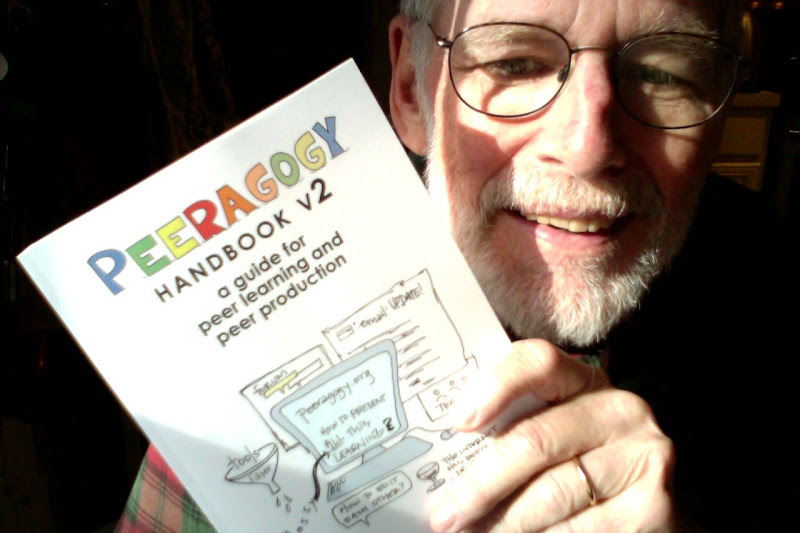
\includegraphics[width=.8\textwidth]{../pictures/george.jpg}
\end{center}

The Second Edition of the \emph{Handbook} came out two years ago.
We've kept at it since then.  This time around, we're kicking things
off with a short workbook that contains a concise guide to the who,
what, when, where, how and why of peeragogy.  We've thoroughly revised
the pattern catalog at the heart of the book, added more case studies,
and made numerous small improvements to the text (and the
typesetting!)  throughout.

\clearpage
 %%%%%%%%%%%%%%%%%%%%  %%%%%%%%%%%%%%%%%%%%  %%%%%%%%%%%%%%%%%%%%

\mainmatter

\part{Introduction} \label{intro-part} %%%%%%%%%%%%%%%%%%%%
\pagestyle{companion}
\chapter[\textbf{Welcome!}]{Welcome to the Peeragogy Handbook}
%
\begin{quote}
We live where no one knows the answer and the struggle is to figure out
the question. {[}1{]}
\end{quote}

Welcome to the \emph{Peeragogy Handbook}! We want to kick things off
with a candid confession: we're not going to pretend that this book is
perfect. In fact, it's not an ordinary book at all. The adventure starts
when you get out your pen or pencil, or mouse and keyboard, and begin
marking it up. It gets kicked into high gear when you join
\emph{Peeragogy in Action}. You'll find a lot of friendly support as you
write, draw, or dance your own peeragogical adventure. But first, what
is \emph{peeragogy}?

Peeragogy is a flexible framework of techniques for peer learning and
peer knowledge production. Whereas pedagogy deals with the transmission
of knowledge from teachers to students, peeragogy is what people use to
produce and apply knowledge together. The strength of peeragogy is its
flexibility and scalability. The learning mind-set and strategies that
we are uncovering in the Peeragogy project can be applied in classrooms,
hackerspaces, organizations, wikis, and interconnected collaborations
across an entire society.

The \emph{Peeragogy Handbook} is a compendium of know how for any group
of people who want to co-learn any subject together, when none of them
is an expert in the particular subject matter -- learning together
without one traditional teacher, especially using the tools and
knowledge available online. What we say in the \emph{Handbook} draws
extensively on our experiences working together on the \emph{Handbook}
-- and our experiences in other collaborative projects that drew us here
in the first place. The best way to learn about peeragogy is to do
peeragogy, not just read about it. Towards that end, coauthors and fans
of the \emph{Handbook} have an active Google+ community, conveniently
called \emph{Peeragogy in Action}. We maintain a regular schedule of
weekly meetings that you're welcome to join. The \emph{Handbook}
includes a short syllabus, which also called ``Peeragogy in Action'',
and you can work through this with your own group as you read through
the book.

You're warmly invited to combine your local projects with the global
effort, and get involved in making the next edition of the
\emph{Handbook}. That doesn't necessarily require you to do extensive
writing or editing. We're always interested in new use cases, tricky
problems, and interesting questions. In fact, our view is that any
question is a good question.

Here are some of the ways in which the current edition of the Handbook
is \emph{not perfect}. You're welcome to add to the list! These are
places where you can jump in and get involved. This list gives a sense
of the challenges that we face putting peeragogy into action.

\hypertarget{scrapbook-of-peeragogical-problems}{%
\section{Scrapbook of Peeragogical
Problems}\label{scrapbook-of-peeragogical-problems}}

\hypertarget{maintaining-a-list-of-useful-resources}{%
\subsection{Maintaining a list of useful
resources}\label{maintaining-a-list-of-useful-resources}}

We include references and recommended reading in the \emph{Handbook},
and there are a lot more links that have been shared in the
\emph{Peeragogy in Action} community. It's a ongoing task to catalog and
improve these resources -- including books, videos, images, projects,
technology, etc. In short, let's ``Reduce, Reuse, Recycle''! As a good
start, Charlotte Pierce has been maintaining a spreadsheet under the
heading ``survey'' in our Google Drive.

\hypertarget{developing-a-really-accessible-diy-tool-kit}{%
\subsection{Developing a really accessible DIY
tool-kit}\label{developing-a-really-accessible-diy-tool-kit}}

A short ``workbook'' containing interviews and some activities follows
this introduction, but it could be much more interactive. Amanda Lyons
and Paola Ricaurte made several new exercises and drawings that we could
include. A more developed workbook could be split off from the handbook
into a separate publication. It would be great to have something simple
for onramping. For example, the workbook could be accompanied by video
tutorials for new contributors.

Paola Ricaurte points out that a really useful book will be easy to
sell. For teachers interested in peeragogy, this needs to be something
that can be use in workshops or on their own, to write in, to think
through issues. We're partway there, but to improve things, we really
need a better set of activities.

The next time Paola or someone else uses the handbook or workbook to run
a workshop, she can say, ``turn to this page, let's answer this
question, you have 10 minutes.'' There are lots of places where the
writing in the handbook could be made more interactive. One technique
Paola and Amanda used was turning ``statements'' from the handbook into
``questions.''

\hypertarget{crafting-a-visual-identity}{%
\subsection{Crafting a visual
identity}\label{crafting-a-visual-identity}}

Amanda also put together the latest cover art, with some collaboration
from Charlotte using inDesign. A more large-scale visual design would be
a good goal for the 4th Edition of the book. Fabrizio Terzi, who made
the handbook cover art for the 1st Edition, has been working on making
our website more friendly. So, again, work is in progress but we could
use your help.

\hypertarget{workflow-for-the-4th-edition}{%
\subsection{Workflow for the 4th
edition}\label{workflow-for-the-4th-edition}}

We've uploaded the content of the book to Github and are editing the
``live'' version of the site in Markdown. For this and previous print
editions, we've converted to LaTeX. There are a number of workflow
bottlenecks: First, people need to be comfortable updating the content
on the site. Second, it would be good to have more people involved with
the technical editing work that goes into compiling for print. Remember,
when we produce an actual physical handbook, we can sell it. In fact,
because all co-authors have transferred their copyright in this book to
the Public Domain, \emph{anyone} can print and sell copies, convert the
material into new interactive forms, or do just about anything with it.

\hypertarget{translations}{%
\subsection{Translations}\label{translations}}

Translating a book that's continually being revised is pretty much a
nightmare. With due respect to the valiant volunteer efforts that have
been attempted so far, it might be more convenient for everyone involved
to just pay professional translators or find a way to foster a
multi-lingual authoring community, or find a way to create a more robust
process of collective translation. Ideas are welcome, and we're making
some small steps here. More on this below.

\hypertarget{next-steps-whats-the-future-of-the-project}{%
\subsection{Next steps? What's the future of the
project?}\label{next-steps-whats-the-future-of-the-project}}

In short: If we make the Handbook even more useful, then it will be no
problem to sell more copies of it. That is one way to make money to
cover future expenses. It's a paradigmatic example for other business
models we might use in the future. But even more important than a
business model is a sense of our shared vision, which is why we're
working on a ``Peeragogy Creed'' (after the Taekwondo creed, which
exists in various forms, one example is {[}2{]}). No doubt you'll find
the first version on peeragogy.org soon! Chapter
\href{./distributed_roadmap.html}{7} contains a further list of
practical next steps for the project.

\hypertarget{references}{%
\subsection{References}\label{references}}

\begin{enumerate}
\def\labelenumi{\arabic{enumi}.}
\item
  Joshua Schimel, 2012. ``Writing Science'', Oxford University Press.
\item
  Taekwondo Student Creed, World Martial Arts Academy,
  \url{http://www.worldtaekwondo.com/handbook.htm}
\end{enumerate}


\newpage

%% \addtocontents{toc}{%
%%  \protect\vspace{-.5cm}%
%% }
%% \includepdf[addtotoc={1,chapter,0,Workbook,chap:workbook},page={1-},offset=5mm 0mm,pagecommand={\pagestyle{companion}}]{peeragogy-workbook-insert.pdf}

\hypertarget{welcome-to-the-peeragogy-workbook}{%
\section{☞ Welcome to the Peeragogy
Workbook!}\label{welcome-to-the-peeragogy-workbook}}

This booklet is designed to introduce you to our fun, exciting world of
peer learning and peer production!! You may already be familiar with
these terms, or they may be new to you. Either way, don't worry!!!

If they are new, consider the following 2 examples.

\begin{enumerate}
\def\labelenumi{\arabic{enumi}.}
\item
  \emph{Peer learning}: Joe Corneli needs to get from the suburbs of
  Chicago to the north side of the city. He gets on the commuter train
  and transfers to the purple ``L'' at Davis Street in Evanston. He
  plans to change to the red line at Howard Street, but the train says
  ``Loop'' and he asks another passenger whether it will stop at Howard.
  She says it will, but that he can save an hour of his time by riding
  express to the city and then coming back two stops! Joe makes it to
  his meeting with Charlie with plenty of time to spare.
\item
  \emph{Peer production}: Two cavewomen see lightning strike a tree and
  produce fire! Walking up to it they notice the heat and think
  ``Wouldn't it be nice to have fire for our family at night!'' Once the
  rain clears, they find some dry sticks and start working together to
  figure out how they can use them to start their own flame. After hours
  of trial and error, BOOM they've got fire! The news travels fast. :)
\end{enumerate}

Peeragogy is an approach to learning and working together on projects
ranging from the mundane to the monumental. Peer learning and peer
production are probably as old as humanity itself, but they take on new
importance in the digital age.

The Peeragogy Project is an informal learning project with members
worldwide. Three members of the project share their welcoming messages
below.

\textbf{Paola Ricaurte Quijano}: Welcome to the Peeragogy Project! We
are a group of enthusiastic people who love to learn and are trying to
find the best ways to learn together.

\textbf{Lisa Snow MacDonald}: Welcome to peeragogy! It's kind of a weird
name, but it's enormously powerful in providing a fresh understanding of
ways of working together.

\textbf{Dorotea Mar}: Your contributions will be really welcome if you
participate respectfully and harmoniously with other peers. It can
change your life and improve your well­being and make everything better.

\hypertarget{a-peeragogy-interview}{%
\section{A Peeragogy Interview}\label{a-peeragogy-interview}}

\hypertarget{introductions}{%
\subsection{Introductions}\label{introductions}}

\textbf{Paola Ricaurte Quijano}: Hi! I'm Paola, I'm from Ecuador. I work
at Tecnológico de Monterrey, a private university in Mexico City, and I
love to learn with everybody!

\textbf{Dorotea Mar}: Hello. I'm in Berlin now and I really like the
peeragogical atmosphere of collaboration and I think we are really
improving ways of collaboration and peer production, so that's why I'm
here.

\textbf{Lisa Snow MacDonald}: Hello. This is Lisa from Los Angeles. My
background is media psychology and I'm interested in peeragogy as it
relates to business.

\emph{What is peer learning/production?}

\textbf{PRQ} Well, peer learning. learning with peers, learning from
peers and trying to make things together or make things happen together.
I think that for me, the most important thing I've learned from this
experience is that you can achieve more when you work together and set
goals together.

\textbf{LSM} I think what peeragogy does is it allows us to recognize
the value of those connections. A lot of other ways of working are more
individualized. It goes back to a concept of 1 + 1 = 2, which is very
rational and very measured and is kind of a dominant way of thinking in
our society today, whereas peer to peer learning and production
recognize the value of those connections. You may not be able to measure
it with a yardstick, but we understand that there is value in those
connections. So it's basically acknowledging that when it comes to
learning/collaborative environments if constructed the right way if
working well it can be 1 + 1 = 3 or 1 + 1 = 4. That type of situation,
which is really different from the way we're used to thinking about
things. And I think that's really the value of what we're doing and the
potential of what we could hopefully unlock.

\emph{More specifically, what is peeragogy and/or what is the Peeragogy
Project?}

\textbf{PRQ} This is a project that began spontaneously. We didn't have
a plan at the beginning. We just talked about the things that concerned
us the most. What do you need if you want to learn with others, how to
learn better? what do you want to learn? Where do you want to learn?
When do you want to learn? Basic questions that can be answered in many
ways. We don't have a strict line. We have a map, maybe, but a map that
can be walked through by many different paths. Paths that you choose can
be related to the people you are working with. I think it's been a great
experience for us. As Lisa said, we have been recognizing the talents
and strengths of every person that has contributed to and participated
in this project.

\textbf{LSM} OK. I'll take my best shot with this. Going back to what I
said earlier and building off what other people have said. Because we
don't have a good mental construct of how this works, and measurement is
difficult. We haven't learned how to measure these connections. I think
what peeragogy and the Peeragogy Project can do is it can establish what
people have said about focusing on the process. It can help people
understand the process better. Because this lack of structure can be
uncomfortable for people. We need to understand when that discomfort is
acceptable, so they don't revert and become counter­productive
participants in the process. The map analogy that Paola just mentioned,
is really good too. It's not about providing a direct path. If you're on
a trip trying to get from LA to Chicago, there's many paths you can
take. It's making sure you're monitoring your resources and you're
taking care of things along the way. You can drift off-course. One plus
one can equal zero if things don't work out well. So, what peeragogy and
the Peeragogy Project can do is to provide some structure and framework
around the unstructured way that things can be done. People trying to
make sure their methods are constructive and beneficial now have some
guidelines and things to watch out for.

\begin{center}\rule{0.5\linewidth}{0.5pt}\end{center}

\hypertarget{example-howard-rheingold-grows-a-learning-network}{%
\subsection{Example: Howard Rheingold Grows a Learning
Network}\label{example-howard-rheingold-grows-a-learning-network}}

``When I started using social media in the classroom, I looked for and
began to learn from more experienced educators. First, I read and then
tried to comment usefully on their blog posts and tweets. When I began
to understand who knew what in the world of social media in education, I
narrowed my focus to the most knowledgeable and adventurous among them.
I paid attention to the people the savviest social media educators paid
attention to. I added and subtracted voices from my attention network,
listened and followed, then commented and opened conversations. When I
found something I thought would interest the friends and strangers I was
learning from, I passed along my own learning through my blogs and
Twitter stream. I asked questions, asked for help, and eventually
started providing answers and assistance to those who seemed to know
less than I. The teachers I had been learning from had a name for what I
was doing --- ``growing a personal learning network.'' So I started
looking for and learning from people who talked about HOW to grow a
``PLN'' as the enthusiasts called them.''

\begin{center}\rule{0.5\linewidth}{0.5pt}\end{center}

\emph{How do you do peeragogy?}

\textbf{DM} I think I do a lot of peeragogy and I'm very happy about it
because I learn so much from my group and from myself in this group that
I like to apply it to other projects that I'm in or things like
co­working and co­living projects. Especially the principle of mutual
respect that still remains after a very long time. And the way we relate
to each other is really nice.

The main principle is mutual respect and openness, and the process. And
in each detail, there is value that we believe in.

Let's say how we manage the Peeragogy Page or Community (See ``How to
Get Involved,'' later in this chapter.). These seem to be details, but
they're actually really important. So if we pay attention to all these,
every little thing matters, and this is how I do it. I try to be very
mindful in all interactions.

\begin{figure}
\centering
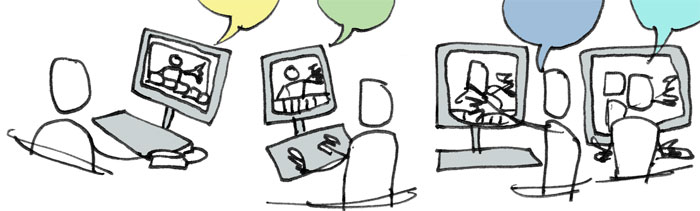
\includegraphics{images/talking.jpg}
\caption{image}
\end{figure}

\begin{center}\rule{0.5\linewidth}{0.5pt}\end{center}

\hypertarget{example-learner-know-thyself.}{%
\subsection{Example: Learner, know
thyself.}\label{example-learner-know-thyself.}}

When he joined the Peeragogy project in 2012, Charles Jeffrey Danoff did
a brief self­evaluation about what makes him interested in learning:

\begin{enumerate}
\def\labelenumi{\arabic{enumi}.}
\item
  Context. As a student, I resisted being groomed for some unforeseeable
  future. I'd rather work toward a specific goal.
\item
  Timing and sequence. I find learning fun when I'm studying something
  as a way to procrastinate another pressing assignment.
\item
  Social reinforcement. Getting tips from peers on how to navigate a
  snowboard around moguls was more fun for me than my Dad showing me the
  proper way to buff the car's leather seats on chore day.
\item
  Experiential awareness. In high school, it was not fun to sit and
  compose a 30-page reading journal on Frankenstein. But owing in part
  to those types of prior experiences, I now find writing pleasurable
  and it's fun to learn how to write better.
\end{enumerate}

\begin{center}\rule{0.5\linewidth}{0.5pt}\end{center}

\textbf{PRQ} I think peeragogy is more like a mind­set. I think we have
to change the way we interact with others and the way we understand the
parameters of learning. For example, I'm a teacher and, of course, my
teaching practice promotes collaborative, creative learning. So, I
expect my students to take responsibility for their own learning by
making decisions about most aspects of the learning process; to program
their own learning goals. They need to learn to effectively employ the
environments (like whiteboards), the activities, and the assessments.
I'm trying to give my learners the tools to decide how, what, and why
they want to learn. For me, it's been a very interesting experience.
Learners often find it unfamiliar to make their own decisions about the
process in a formal environment. At the beginning of the semester,
students are given everything and usually just follow guidelines and
criteria. I have been trying to change this dynamic. Students feel
insecure, because they really do not know how or what they want to do.
So, that process of making decisions together becomes very rich and very
meaningful.

\begin{figure}
\centering
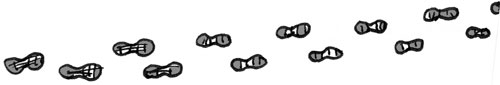
\includegraphics{images/footprints.jpg}
\caption{image}
\end{figure}

\begin{center}\rule{0.5\linewidth}{0.5pt}\end{center}

\hypertarget{example-metacognition-and-mindfulness}{%
\subsection{Example: Metacognition and
Mindfulness}\label{example-metacognition-and-mindfulness}}

\begin{quote}
Alan Schoenfeld: ``What (exactly) are you doing? Can you describe it
precisely? Why are you doing it? How does it fit into the solution? How
does it help you? What will you do with the outcome when you obtain
it?'' {[}1{]}
\end{quote}

\begin{center}\rule{0.5\linewidth}{0.5pt}\end{center}

\emph{When do you do peeragogy?}

\textbf{DM} I think I'm always practicing it. I really like that during
the weekly hangouts we don't usually have rigid agendas. We just get
creative and let ideas connect and flow. And whatever happens it's the
right thing. We just work together and somehow the right things happen.
I think we're always doing peeragogy when we pursue activities and
projects in open, collaborative ways without imposing too much structure
or heirarchy.

\textbf{PRQ} I agree with Dorotea. The where and when questions are
related. If you're thinking about where, you're thinking about when. So
if ``where'' is everywhere, and ``when'' is always, I agree. Anywhere,
everywhere, all the time. It's an ongoing process. If you believe in
peeragogy as a way of doing things or making things happen, you cannot
switch back and forth betweeen two different personas and say, ``I'm not
working with peeragogy now,'' or ``I am applying peeragogy now.''

\textbf{LSM} I'm familiar with the business world where there are
distinct personalities. For example there are people who tend to be more
collaborative just by nature, who tend to adapt and to prefer a
peeragogical model. Other personalities are less so, and that's why what
we're doing here is valuable. In practice, there's seldom a conscious
recognition of these different styles of working. In a business
environment, there are different motivators, different personalities
tossed together, all united by a single goal. So understanding
peeragogical vs.~heirarchical practices, and raising the differences to
the surface, could be very valuable in pursuing the goal of making
people's lives better in the business environment.

\textbf{DM} There are many collaborative projects that aim to do
something similar to this, but, in a sense, focus on different aspects
of the process, and maybe not on such an abstract level as we might.

Some people have natural peeragogical tendencies, and some people are
less transparent in the way they do things. For me, peeragogy is really
beneficial, especially for collaborative projects. Everybody works and
learns differently, so if everyone became increasingly aware of how they
and others work and learn, of how peergogy functions, and how it all
fits into a bigger picture, many tasks would not only be more
efficiently done, but also much more enjoyable. It's also beneficial if
everyone focusses on a bigger picture instead of focussing only on their
part of it, and if attention is drawn to all that could be done in a
peeragogical way.

\begin{center}\rule{0.5\linewidth}{0.5pt}\end{center}

\hypertarget{example-jay-cross-on-setting-sail}{%
\subsection{Example: Jay Cross on Setting
Sail}\label{example-jay-cross-on-setting-sail}}

``If I were an instructional designer in a moribund training department,
I'd polish up my resume and head over to marketing. Co­learning can
differentiate services, increase product usage, strengthen customer
relationships, and reduce the cost of hand­holding. It's cheaper and
more useful than advertising. But instead of just making a copy of
today's boring educational practices, build something based on
interaction and camaraderie, perhaps with some healthy competition
thrown in. Again, the emphasis should always be on learning in order to
do something!''

\begin{center}\rule{0.5\linewidth}{0.5pt}\end{center}

\emph{Why do you do peeragogy?}

\textbf{PRQ} Why? Well, as said before, I believe in peeragogy. I
believe it's a good way to learn. Maybe it's the best way. I think I
wasn't aware of that before joining the group. I have always been a
self­learner, I have been working mostly alone. After I began working
with the group, I understood that you grow working with a group. You
achieve things that you aren't able to achieve alone. I think there's a
growing awareness of the value of collaboration in every setting and
environment. There are more and more learning communities around the
world where people are also learning that making decisions together and
working together are the best way to be in this world! I think as we
live through hard times, we increasingly need a sense that we are not
alone and that we cannot solve problems alone.

\emph{How did you join the Peeragogy project?}

\textbf{PRQ} After taking Howard Rheingold's course on Mind Amplifiers
in 2012 we were invited to join this group. There was no plan, just an
open question of how to best learn with others.\\
That's how it began. We had lots of sessions and discussed a wide range
of issues. The Peeragogy Handbook (http://peeragogy.org) was the product
of that process. We've been working with the Handbook, releasing a new
version every year and trying to figure out what might be the best way
to go forward and what the future of our collaboration as a group/team
might be.

\textbf{LSM} A couple friends of mine were involved in P2P learning.
They were invited to a conference at UCI. Howard was at the event and
they were familiar with him and his work. We ended up in an obscure
classroom and he started talking about principles that were peeragogy
related, while I don't know if it provided much value to my friends, it
sounded a lot like what I saw in business and he mentioned the group. So
after that, I met everyone here and it's been pretty random.

\textbf{DM} I think many paths led to my involvement. I have a lot of
academic experience and was doing research on Open Science. I had always
wanted to improve the way things work and somehow I wanted to do it more
creatively. I resonated a lot with the Peeragogy Project on many levels,
so somehow I just joined, I think it was serendipity of some kind.

This interview was conducted on December 15th, 2014. The transcript was
edited. You can watch the whole interview online at
http://is.gd/peeragogyworkbook\_interviews. (49 Minutes)

We've given you some examples but this wouldn't be a proper workbook
without an exercise. Pick at least one thing you're good at and one
thing you want to improve on from the selection below (or write in your
own alternative answers):

\begin{center}\rule{0.5\linewidth}{0.5pt}\end{center}

\hypertarget{exercise-how-do-you-see-yourself-fitting-in}{%
\section{Exercise: How do you see yourself fitting
in?}\label{exercise-how-do-you-see-yourself-fitting-in}}

\hypertarget{potential-roles-in-your-peerlearning-project}{%
\subsection{Potential roles in your peer­learning
project}\label{potential-roles-in-your-peerlearning-project}}

\begin{itemize}
\tightlist
\item
  Worker, Team Member, Co­Manager, Manager, Co­Leader, Leader
\item
  Reviewer, Editor, Author, Content Processor, Content Creator,
\item
  Presentation Creator, Designer, Graphics, Applications
\item
  Attendee, Participant, Coordinator, Project Manager, Planner
\item
  Mediator, Moderator, Facilitator, Proponent, Advocate, Representative,
  Contributor , Activist,
  {~~~~~~~~~~~~~~~~~~~~~~~~~~~~~~~~~~~~~~~~~~~~~~~~}
\end{itemize}

\hypertarget{potential-contributions}{%
\subsection{Potential contributions}\label{potential-contributions}}

\begin{itemize}
\tightlist
\item
  Create, Originate, Research, Aggregate
\item
  Develop, Design, Integrate, Refine, Convert
\item
  Write, Edit, Format,
  {~~~~~~~~~~~~~~~~~~~~~~~~~~~~~~~~~~~~~~~~~~~~~~~~}
\end{itemize}

\hypertarget{potential-motivations}{%
\subsection{Potential motivations}\label{potential-motivations}}

\begin{itemize}
\tightlist
\item
  Acquisition of training or support in a topic or field;
\item
  Building relationships with interesting people;
\item
  Finding professional opportunities through other participants;
\item
  Creating or bolstering a personal network;
\item
  More organized and rational thinking through dialog and debate;
\item
  Feedback about performance and understanding of the topic.
\item
  {~~~~~~~~~~~~~~~~~~~~~~~~~~~~~~~~~~~~~~~~~~~~~~~~~~~~~~~~~~~~~~~~~~~~~~~~~~~~~~~~~~~~~~~~~~~~~~~~~~~~~~~~~~~~~~~~~~~~~~~~~~~~~~~~}
\end{itemize}

\begin{center}\rule{0.5\linewidth}{0.5pt}\end{center}

Visuals by Amanda Lyons (http://visualsforchange.com/). Booklet by
Charlie Danoff, Paola Ricaurte Quijano, Lisa Snow MacDonald, Dorotea
Mar, Joe Corneli and Charlotte Pierce.

Prepared for Public Domain Day 2015 on January 1st, 2015.

See \url{https://github.com/Peeragogy/Peeragogy.github.io} for the
``behind the scenes''.

\begin{figure}
\centering
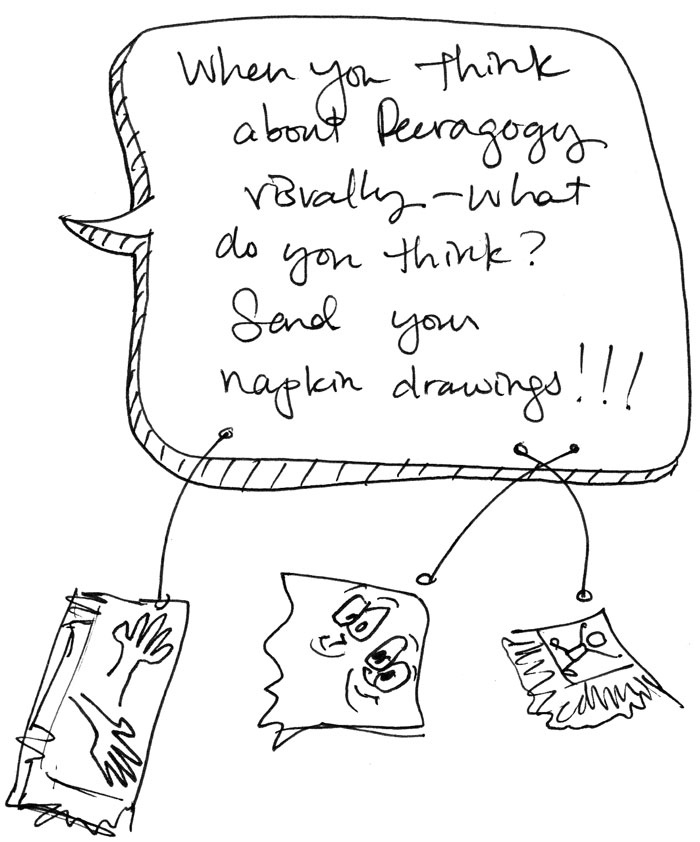
\includegraphics{images/napkin-drawings.jpg}
\caption{image}
\end{figure}

\hypertarget{reference}{%
\section{Reference}\label{reference}}

\begin{enumerate}
\def\labelenumi{\arabic{enumi}.}
\tightlist
\item
  Schoenfeld, A. H. (1987). What's all the fuss about metacognition? In
  A. H. Schoenfeld (Ed.), Cognitive science and mathematics education
  (pp.~189­215). Hilldale, NJ: Lawrence Erlbaum Associates.
\end{enumerate}


\chapter[\textbf{Chapter Summaries}]{Chapter Summaries}
%
\hypertarget{motivation}{%
\subsubsection{Motivation}\label{motivation}}

You might wonder why we're doing this project -- what we hope to get out
of it as volunteers, and how we think what we're doing can make a
positive difference in the world. Have a look at this chapter if you,
too, are thinking about getting involved in peeragogy, or wondering how
peeragogy can help you accelerate your learning projects.

\hypertarget{case-study-5ph1nx.}{%
\paragraph{\texorpdfstring{\emph{Case Study:
5PH1NX.}}{Case Study: 5PH1NX.}}\label{case-study-5ph1nx.}}

This example focuses on the interrelationship of pedagogy and peeragogy
in a high school English class, when students are encouraged to find and
share creative ways to learn. Explore this case study for ideas and
encouragement for your own learning adventures.

\hypertarget{peeragogy-in-practice}{%
\subsubsection{Peeragogy in Practice}\label{peeragogy-in-practice}}

Here we describe some of the interaction patterns that we've encountered
time and time again in the Peeragogy project. You can use the ideas in
this chapter as a starter-kit for your own experiments with peeragogy
right away. Sharing -- and revising -- patterns is one of the key
activities in peeragogy, so you will likely want to revisit this chapter
several times as you look through the rest of the book. Don't forget
your red pen or pencil, because you'll also want to tailor the patterns
we describe here to suit.

\hypertarget{case-study-swats.}{%
\paragraph{\texorpdfstring{\emph{Case Study:
SWATS.}}{Case Study: SWATS.}}\label{case-study-swats.}}

We present another example of peer learning in a classroom setting,
focusing on the process of improving overall student performance with
the help of a group of student experts. After describing the case study
in general terms, we then re-analyze it using our pattern tools to show
how examples like this can be integrated into our project.

\hypertarget{convening-a-group}{%
\subsubsection{Convening a Group}\label{convening-a-group}}

This chapter is about how to begin your own peeragogical project. You
can also use the ideas described here to strengthen an existing
collaboration. Simple but important questions will inspire unique
answers for you and your group. In short: who, what, when, where, why,
and how? Use this chapter to help design and critique your project's
roadmap.

\hypertarget{play-learning.}{%
\paragraph{\texorpdfstring{\emph{Play \&
Learning.}}{Play \& Learning.}}\label{play-learning.}}

What makes learning fun? Just as actors learn their roles through the
dynamic process of performance, In other words, the more we engage with
a topic, the better we learn it and the more satisfying - or fun - the
process becomes.

\hypertarget{k-12-peeragogy.}{%
\paragraph{\texorpdfstring{\emph{K-12
Peeragogy.}}{K-12 Peeragogy.}}\label{k-12-peeragogy.}}

The key to becoming a successful `connected educator-learner' involves
spending the time needed to learn how to learn and share in an open,
connected environment. Once you make the decision to enter into a
dialogue with another user, you become a connected educator/learner and
tap into the power of networks to distribute the load of learning.
Depending on their age, you can even facilitate an awareness of peer
networks among your students.

\hypertarget{p2p-self-organizing-learning-environments.}{%
\paragraph{\texorpdfstring{\emph{P2P Self-Organizing Learning
Environments.}}{P2P Self-Organizing Learning Environments.}}\label{p2p-self-organizing-learning-environments.}}

This section invites an exploration of support for self-organized
learning in global and local networks. Emergent structures can create
startling ripple effects.

\hypertarget{organizing-a-learning-context}{%
\subsubsection{Organizing a Learning
Context}\label{organizing-a-learning-context}}

Peer learning is sometimes organized in ``courses'' and sometimes in
``spaces.'' We present the results of an informal poll that reveals some
of the positive and some of the negative features of our own early
choices in this project.

\hypertarget{adding-structure-with-activities.}{%
\paragraph{\texorpdfstring{\emph{Adding Structure with
Activities.}}{Adding Structure with Activities.}}\label{adding-structure-with-activities.}}

The first rule of thumb for peer learning is: announce activities only
when you plan to take part as a fully engaged participant. Then ask a
series of questions: what is the goal, what makes it challenging, what
worked in other situations, what recipe is appropriate, what is
different about learning about this topic?

\hypertarget{student-authored-syllabus.}{%
\paragraph{\texorpdfstring{\emph{Student Authored
Syllabus.}}{Student Authored Syllabus.}}\label{student-authored-syllabus.}}

This chapter describes various methods for co-creating a curriculum. If
you're tasked with teaching an existing curriculum, you may want to
start with a smaller co-created activity; but watch out, you may find
that co-creation is habit forming.\footnote{Quick tip: if you create a
  syllabus, share it!}

\hypertarget{case-study-collaborative-explorations.}{%
\paragraph{\texorpdfstring{\emph{Case Study: Collaborative
Explorations.}}{Case Study: Collaborative Explorations.}}\label{case-study-collaborative-explorations.}}

This chapter describes collaborative peer learning among adult students
in the Master's program in Critical and Creative Thinking at University
of Massachusetts in Boston. The idea in the collaborative explorations
is to encourage individuals pursuing their own interests related to a
predetermined topic, while supporting learning of everyone in the group
through sharing and reflection. These interactions of supportive mutual
inquiry evolve the content and structure within a short time frame and
with open-ended results.

\hypertarget{cooperation}{%
\subsubsection{Cooperation}\label{cooperation}}

Sometimes omitting the figurehead empowers a group. Co-facilitation
tends to work in groups of people who gather to share common problems
and experiences. The chapter suggests several ways to co-facilitate
discussions, wiki workflows, and live online sessions. Conducting an
``after action review'' can help expose blind spots.

\hypertarget{the-workscape.}{%
\paragraph{\texorpdfstring{\emph{The
Workscape.}}{The Workscape.}}\label{the-workscape.}}

In a corporate workscape, people are free-range learners: protect the
learning environment, provide nutrients for growth, and let nature take
its course. A workscape features profiles, an activity stream, wikis,
virtual meetings, blogs, bookmarks, mobile access and a social network.

\hypertarget{participation.}{%
\paragraph{\texorpdfstring{\emph{Participation.}}{Participation.}}\label{participation.}}

Participation grows from having a community of people who learn
together, using a curriculum as a starting point to organize and trigger
engagement. Keep in mind that participation may follow the 90/9/1
principle (lurkers/editors/authors) and that people may transition
through these roles over time.

\hypertarget{designs-for-co-working.}{%
\paragraph{\texorpdfstring{\emph{Designs For
Co-Working.}}{Designs For Co-Working.}}\label{designs-for-co-working.}}

Designing a co-working platform to include significant peer learning
aspects often requires a new approach. This chapter describes the
initial steps of converting an existing online encyclopedia project into
a peer learning platform.

\hypertarget{assessment}{%
\subsubsection{Assessment}\label{assessment}}

``Usefulness'' is an appropriate metric for assessment in peeragogy,
where we're concerned with devising our own problems rather than than
the problems that have been handed down by society. We use the idea of
return on investment (the value of changes in behavior divided by the
cost of inducing the change) to assess the Peeragogy project itself, as
one example.

\hypertarget{researching-peeragogy.}{%
\paragraph{\texorpdfstring{\emph{Researching
peeragogy.}}{Researching peeragogy.}}\label{researching-peeragogy.}}

This chapter is based on a ``found manuscript'' created by one of us as
an undergraduate. It looks at the challenges that are associated with
combining the roles of student, teacher, and researcher. It shows the
relevance of peer support, and also illustrates the important factor of
time in the evolution of an idea.

\hypertarget{technologies-services-and-platforms}{%
\subsubsection{Technologies, Services, and
Platforms}\label{technologies-services-and-platforms}}

Issues of utility, choice, coaching, impact and roles attach to the wide
variety of tools and technologies available for peer learning. Keys to
selection include the features you need, what people are already using,
and the type of tool (low threshold, wide wall, high ceilings) used for
collaboration.

\hypertarget{forums.}{%
\paragraph{\texorpdfstring{\emph{Forums.}}{Forums.}}\label{forums.}}

Forums are web-based communication media that enable groups of people to
conduct organized multimedia discussions about multiple topics over a
period of time, asynchronously. A rubric for evaluating forum posts
highlights the value of drawing connections. This chapter includes tips
on selecting forum software.

\hypertarget{wiki.}{%
\paragraph{\texorpdfstring{\emph{Wiki.}}{Wiki.}}\label{wiki.}}

A wiki is a website whose users can add, modify, or delete its content
via a web browser. Pages have a feature called ``history'' which allows
users to see previous versions and roll back to them. This chapter
includes tips on how to use a wiki and select a wiki engine, with
particular attention to peer learning opportunities.

\hypertarget{real-time-meetings.}{%
\paragraph{\texorpdfstring{\emph{Real-time
meetings.}}{Real-time meetings.}}\label{real-time-meetings.}}

Web services enable broadband-connected learners to communicate in real
time via audio, video, slides, whiteboards, chat, and screen-sharing.
Possible roles for participants in real-time meetings include searchers,
contextualizers, summarizers, lexicographers, mappers, and curators.
This mode of interaction supports emergent agendas.

\hypertarget{connectivism-in-practice.}{%
\paragraph{\texorpdfstring{\emph{Connectivism in
Practice.}}{Connectivism in Practice.}}\label{connectivism-in-practice.}}

Massive Open Online Courses (MOOCs) are decentralized online learning
experiences: individuals and groups create blogs or wikis and comment on
each other's work, often with other tools helping find information.

\hypertarget{resources}{%
\subsubsection{Resources}\label{resources}}

Here we present a sample syllabus for bringing peer learning to life,
recommended reading and tips on writing for The Handbook, as well as our
Creative Commons Zero 1.0 Universal (CC0 1.0) Public Domain Dedication.


\part{Motivation} \label{motivation-part} %%%%%%%%%%%%%%%%%%%%
%
\chapter[\textbf{Why we're doing this}]{Why we're doing this}
\begin{quote}
Participants must bring self-knowledge and no small measure of honesty
to the peer-learning project in order to accurately enunciate their
motivations.~If everyone in your peer learning project asks ``What
brings me here?'' ``How can I contribute?'' and ``How can I contribute
more effectively?'' things will really start percolating. Test this
suggestion by asking these questions yourself and taking action on the
answers!
\end{quote}

Some of the primary motivators reported by participants in the Peeragogy
project include:

\begin{enumerate}
\def\labelenumi{\arabic{enumi}.}
\item
  Acquisition of training or support in a topic or field;
\item
  Building relationships with interesting people;
\item
  Finding professional opportunities by networking;
\item
  Creating or bolstering personal connections;
\item
  More organized and rational thinking through dialog and debate
  {{[}1{]}};
\item
  Feedback about their own performance and understanding of the topic.
\end{enumerate}

We've seen that different motivations can affect the vitality of the
peeragogical process and the end result for the individual participant.~
And different participants definitely have different motivations, and
the differences can be surprising: for instance, if you're motivated by
social image, you may not be so interested in reciprocity, and vice
versa {{[}2{]}}. Motivations come with associated risks. For example,
one may be reluctant to mention business aspirations in a volunteer
context for fear of seeming greedy or commercial. Whether or not
potential peeragogues eventually decide to take on the risk depends on
various factors.~ Actions that typify inappropriate behavior in one
culture might represent desirable behavior in another. Motivations often
come out of the closet through conflict; for example, when one learner
feels offended or embarrassed by the actions of another.

When it comes to primary motivators, it seems some people are more
motivated by the \emph{process} and some people are motivated by the
\emph{end result}. A lot of the motivations mentioned in the list above
are process-oriented. A process orientation is exemplified in the
following quote:

\begin{quote}
\textbf{Philip Spalding}: ``The idea of visiting a garden together in a
group to learn the names of flowers might have been the original
intention for forming a Garden Group. The social aspect of having a day
out might be goal of the people participating.''
\end{quote}

The basic dichotomy between process and product can be a source of
tension. Some people are OK with a process that is long and drawn out --
because they're mostly there for the process itself anyway. Others will
only tolerate with a slight delay as long as the important end result
remains in sight. Without a clear understanding and a good balance
between these different core motivators, there will be conflict.

People often come to a collaboration with their own motivation in mind
(with more or less clarity from case to case). They don't always step
back to realise that other people are coming from the point of view of
another often very different motivation. It never hurts to ask,
especially when conflict rears up. Accordingly, especially for those
readers who are interested in the \emph{end results} and
\emph{applications} of peeragogy, and not yet steeped in the process,
here's what we ask:

\emph{What are the problems you're grappling with? How do you think
``peer learning'' and ``peer production'' could help you? Would you be
willing to share some of the techniques that you use, and to learn
together with us?}

\hypertarget{example-peeragogy-editor-charlotte-pierce}{%
\section{Example: Peeragogy editor Charlotte
Pierce}\label{example-peeragogy-editor-charlotte-pierce}}

Basically, I'm here because as an early adopter and admitted gadget
freak, I find it fun and rewarding to explore new technologies and
topics that I feel have a practical or exciting application. But I have
some some other motivations that subtly co-exist alongside my eagerness
to explore and learn.

Howard Rheingold's reputation as an innovator and internet pioneer got
my attention when he announced his Think-Know Tools course on Facebook
in 2012. I had known of Howard from the 1990's when I was a member of
The WELL (Whole Earth `Lectronic Link). I was curious to see what Howard
was up to, so I signed onto the wiki site, paid my \$300, and took the
course starting in October.

Looking back, I realize we were practicing Peeragogy throughout the TKT
course, though at the time I hardly knew peer learning from a pickle. In
late November, missing the camaraderie and challenge of TKT, I stepped
over to check out the \emph{Peeragogy Handbook}.

Which brings me to motivations in signing on to Peeragogy. Since Howard
and several Think-Know Tools co-learners were already dedicating their
time here and their work looked innovative and exciting, I suspected
they might be onto something that I wanted to be a part of. Plus, my
brain was primed by the TKT experience. ``What if a diverse group of
people could learn a subject with little or no cost and not a lot of
barriers to entry,'' I thought. ``What if their own experience qualified
them to join, contribute, and learn.''

I also thought there might be a chance to meet some potential business
partners or clients there - but if not, the experience looked rewarding
and fun enough for me to take the risk of no direct remuneration. There
was no up front cost to me, and a wealth of knowledge to gain as a part
of something new and exciting. These are always big draws for me. I
wanted to be in on it, and nobody was telling me I couldn't!

My projections proved correct. The participants already on board were
gracious in welcoming me to Peeragogy, patient in getting me up to
speed, and persistent in coaxing me into using the tools central to the
project. I connected, learned, grew, and contributed. Now I'm on the
brink of starting a peer learning project of my own in my publishing
organization, IPNE.org. Stay tuned!

\hypertarget{example-cafes-schools-workshops}{%
\section{Example: Cafes, schools,
workshops}\label{example-cafes-schools-workshops}}

Suppose we wanted to make Peeragogy into a model that can be used in
schools, libraries, and so forth, worldwide - and, in fact we do! ~How
can we bring the basic Peeragogy motivations to bear, and make a
resource, plan of action, and process that other people can connect
with? ~In brief, how do we build peer learning into the curriculum,
providing new insight from the safety of the existing structure?

One concrete way to implement these broad aims would be to make a
peeragogy-oriented \emph{development} project whose goal is to set up a
system of internet cafes, schools, or workshops in places like China or
Africa, where people could go to collaborate on work or to learn
technical subjects. Students could learn on the job. It seems reasonable
to think that investors could make a reasonable profit through
``franchises,'' hardware sales, and so forth -- and obviously making
money is a motivation that most people can relate to.

In developing such a project, we would want to learn from other similar
projects that already exist. ~For example, in Chicago, State Farm
Insurance has created a space called the
``\href{https://www.nextdoorchi.com/}{Next Door Cafe}'' that runs
community events. One of their offerings is free financial coaching,
with the explicit agreement that the issues you discuss return to State
Farm as market research.

\begin{quote}
\textbf{State Farm Insurance}: ``Free? Really. Yes, because we're
experimenting. We want to learn what people really want. Then, we'll
shoot those wants back to the Farm. We help you. You help us innovate.
We're all smarter for it. We think it's a win-win.''
\end{quote}

Thus, Next Door Cafe forms part of a system to exploit the side-effects
of interpersonal interactions to create a system that learns.~ A peer
learning example from the opposite side of the world started in a slum
next to New Delhi where Sugata Mitra gave children a computer and they
self organized into a learning community and taught themselves how to
use the machine and much more.

\begin{quote}
\textbf{Sugata Mitra}: ``I think what we need to look at is we need to
look at learning as the product of educational self-organization. If you
allow the educational process to self-organize, then learning emerges.
It's not about making learning happen. It's about letting it happen.''
\end{quote}

In 2014, we tried a similar experiment. We asked: Can we build a
``\href{http://commonsabundance.net/docs/help-build-the-peeragogy-accelerator-work-in-progress/}{Peeragogy
Accelerator}'' for a half-dozen peer learning projects, each of which
defines their own metrics for success, but who come together to offer
support and guidance, using the \emph{Peeragogy Handbook} as a resource?
We tried that with several our own projects, and benefitted from the
peer support. Several months later, we found the Accelerator format even
more exciting when we ran a one-off series focusing on Sagarika Bhatta's
research on adaptation to climate change in Nepal. Our sense is that
peeragogy could be useful for building a global support network around
just about any project. Peeragogy can support a culture of real
engagement, rather than ``clicktivism,'' and the direct exchange of
critically-assessed effort rather than often-inefficient donations of
cash {[}3{]}.

\hypertarget{references}{%
\subsection{References}\label{references}}

\begin{enumerate}
\def\labelenumi{\arabic{enumi}.}
\item
  Hugo Mercier and Dan Sperber (2011). Why do humans reason? Arguments
  for an argumentative theory, \emph{Behavioral and Brain Sciences}, 34,
  57-111.
\item
  Jérôme~Hergueux (2013).
  \href{https://cyber.law.harvard.edu/interactive/events/luncheons/2013/11/jerome}{Cooperation
  in a Peer Production Economy: Experimental Evidence from Wikipedia},
  talk presented at the Berkman Center for Internet and Society.
\item
  Kevin Edmonds (2012). Beyond Good Intentions: The Structural
  Limitations of NGOs in Haiti. \emph{Critical Sociology}, 39(3).
\end{enumerate}

%
\chapter[\textbf{Case Study: 5PH1NX}]{Case Study: 5PH1NX}\label{sphinx-beginning}
%
\begin{quote}
5PH1NX: 5tudent Peer Heuristic for 1Nformation Xchange - we think of it
as a ``curiously trans-media'' use case in peeragogical assessment.
\end{quote}

Over the last several decades, technology has driven massive shifts in
the way we communicate and collaborate. Information technology,
socioeconomic trends, an increasingly complex and uncertain future, and
the widely perceived failure of our school system to adequately prepare
students are contributing factors in an emerging discourse that seeks to
align learning with our rapidly changing culture.

Open Source Learning and Peeragogy, two emerging theoretical frameworks
in this discourse, leverage end-to-end user principles of communication
technology to facilitate peers learning together and teaching each
other. In both traditional and liminal learning communities, one of the
major points of contact between education and societal culture is the
purposeful use of assessment. The processes of giving, receiving, and
applying constructive critique makes learners better thinkers,
innovators, motivators, collaborators, coworkers, friends, relatives,
spouses, teammates, and neighbors. Implementing peer-based assessment
can be problematic in schooling institutions where evaluative authority
is traditionally conflated with hierarchical authority, and where
economic and political influences have focused attention on summative,
quantitative, standardized measurement of learning and intelligence.

This is the story of how one learning community is adopting Open Source
Learning and Peeragogical principles to decentralize and enrich the
assessment process.

\begin{quote}
\textbf{Aldous Huxley}: ``Knowledge is acquired when we succeed in
fitting a new experience into the system of concepts based upon our old
experiences. Understanding comes when we liberate ourselves from the old
and so make possible a direct, unmediated contact with the new, the
mystery, moment by moment, of our existence.''
\end{quote}

\hypertarget{enter-5ph1nx}{%
\subsection{Enter 5PH1NX}\label{enter-5ph1nx}}

On Monday, April 2, 2011, students in three English classes at a
California public high school discovered anomalies in the day's entry on
their course blog. (Reminder: not so long ago this sentence would have
been rightly interpreted as being science fiction.) The date was wrong
and the journal topic was this:

\begin{quote}
In The Principles of Psychology (1890), William James wrote, ``The
faculty of voluntarily bringing back a wandering attention, over and
over again, is the very root of judgment, character and will. No one is
\emph{compos sui} if he have it not. An education which should improve
this faculty would be the education par excellence.'' How have your
experiences in this course helped you focus your attention? What do you
still need to work on? What elements of the following text (from Haruki
Murakami's \emph{1Q84}) draw your attention and help you construct
meaning?\\
The driver nodded and took the money. ``Would you like a receipt?'' ``No
need. And keep the change.'' ``Thanks very much,'' he said. ``Be
care\textbf{f}ul, it looks windy out there. Don't sl\textbf{i}p.''
``I'll be careful,'' Aomame said. ``A\textbf{n}d also,''
the~\textbf{d}river said, facing~\textbf{t}he mirror, ``please remember:
t\textbf{h}ings are not what they seem.''~ Things are not what they
seem, Aomame repeated mentally. ``What do you mean by that?'' she asked
with knitt\textbf{e}d brows. The driver chose his words carefully:
``It's~\textbf{j}ust that y\textbf{o}u're about to do something out of
the ordinary. Am I right? People do not ordinarily climb down the
emergency stairs of the Metropolitan Expressway in the middle of the
day-- especially women.'' ``I suppose you're right.'' ``Right. And after
you do something like that, the everyday loo\textbf{k}~of things might
seem to chang\textbf{e}~a little. Things may
look~\emph{diffe\textbf{r}ent}~to you than they did before. I've had
that experience myself. But don't let appearance\textbf{s} fool you.
There's always only one reality.''
\end{quote}

\hypertarget{find-the-jokers}{%
\subsection{Find the jokers}\label{find-the-jokers}}

The jokers were real and hidden (without much intent to conceal) around
the classroom and in students' journals. Students found them and asked
questions about the letters in bold; the questions went unanswered. Some
thought it was just another of their teacher's wild hair ideas. Although
they didn't know it yet they were playing the liminal role that Oedipus
originated in mythology. Solving the riddle would enable them to usher
out an old way of thinking and introduce the new.

The old way: An authority figure sets the rules, packages the
information for a passive audience, and unilaterally evaluates each
learner's performance. In that context, peeragogical assessment might be
introduced with a theoretical framework, a rubric, and a lesson plan
with input, checks for understanding, and guided practice as a
foundation for independent work.

The new way: In Open Source Learning the learner pursues a path of
inquiry within communities that function as end-to-end user networks.
Each individual begins her learning with a question and pursues answers
through an interdisciplinary course of study that emphasizes multiple
modalities and the five Fs: mental Fitness, physical Fitness, spiritual
Fitness, civic Fitness, and technological Fitness. Learners collaborate
with mentors and receive feedback from experts, community-based peers,
and the public. They are the heroes of learning journeys. Heroes don't
respond to syllabi. They respond to calls to adventure. Open Source
Learning prepares students for the unforeseen.

By the time they met the 5PH1NX students had learned about habits of
mind, operating schema, digital culture and community, self-expression,
collaboration, free play, autonomy, confidence/trust/risk, and
resilience. These ideas had been reinforced through nonfiction articles
and literary selections such as Montaigne's Essays, Plato's Allegory of
the Cave, Shakespeare's Hamlet, Sartre's No Exit and others. The first
poem assigned in the course was
Bukowski's~``\href{http://www.youtube.com/watch?v=bHOHi5ueo0A}{Laughing
Heart}''. \emph{The Gods will offer you chances. Know them. Take them.}

So it is with knowledge and understanding. Today we are presented with
an overwhelming, unprecedented quantity and variety of data in our
physical and virtual lives; to cope we must improve the ways we seek,
select, curate, analyze, evaluate, and act on information.

On the back of each Joker card was a QR code that linked to a blog page
with riddles and clues to a search. At this point students realized they
were playing a game. A tab on the blog page labeled ``The Law'' laid out
the rules of engagement:

\hypertarget{this-is-the-law}{%
\subsection{This is The Law}\label{this-is-the-law}}

\begin{enumerate}
\def\labelenumi{\arabic{enumi}.}
\item
  You cannot ``obey'' or ``break'' The Law. You can only make good
  decisions or bad decisions.
\item
  Good decisions lead to positive outcomes.
\item
  Bad decisions lead to suffering.
\item
  Success requires humanity.
\item
  ``For the strength of the Pack is the Wolf, and the strength of the
  Wolf is the Pack.'' -Rudyard Kipling
\item
  ``The Way of the sage is to act but not to compete.'' -Lao Tzu
\item
  Be honorable.
\item
  Have fun.
\item
  Question.
\item
  \emph{Sapere aude}.
\end{enumerate}

This is The Law. After a second set of on-campus and blog quests,
students noticed a shift in 5PH1NX. A couple of weeks before the first
clue was published, during a Socratic seminar on Derrida's concept of
Free Play, a student said, ``We learn best when adults take away the
crutches and there is no safety net.''? The quote was used in the next
clue; students began to realize that the game was not pre-determined.
5PH1NX was evolving in response to their contributions. This is a
manifestation of the hackneyed writing cliché: show, don't tell. The
student's comment was a call to action. The Feats of Wisdom were
designed to engage learners over a vacation break in fun, collaborative,
social media-friendly missions that required engagement in the
community, expansion of their personal learning networks, and
documentation on their blogs. For example:

\hypertarget{feat-1.}{%
\paragraph{FEAT \#1.}\label{feat-1.}}

\emph{Buy a ticket to ``The Hunger Games'' (or any other movie that's
likely to draw a large, young, rowdy audience). Before the lights dim
and the trailers begin, walk to the screen, turn to the audience, and in
a loud, clear voice, recite the ``To be, or not to be\ldots{}''
soliloquy from Hamlet (don't worry if you make a couple mistakes, just
be sure you make it all the way to, ``Be all my sins
remembered.'').~\href{http://alarhsenglitcomp.blogspot.com/2012/12/feats-of-wisdom-1_15.html}{Capture
the event on video \& post it to your blog.}}

Students had been using the Internet without an Acceptable Use Policy
all year; such policies are one-to-many artifacts of a central authority
and far weaker than community norms. So rather than introduce ``rules''
5PH1NX simply provided a reminder of the client-side responsibility.

\hypertarget{the-emergence-of-peeragogical-assessment}{%
\subsection{The Emergence of Peeragogical
Assessment}\label{the-emergence-of-peeragogical-assessment}}

The third page on the Feats of Wisdom blog was entitled
\emph{Identifying and Rewarding Greatness}, where learners were greeted
with the following paragraph:

\begin{quote}
If you see something that was done with love, that pushed the
boundaries, set the standard, broke the mold, pushed the envelope,
raised the bar, blew the doors off, or rocked in some previously
unspecified way, please bring it to the attention of the tribe by
posting a link to it {{[}here{]}}.
\end{quote}

No one did. Instead, they started doing something more effective. They
started building. One student hacked the entire game and then created
her own version. Other students began to consider the implications for
identifying and rewarding greatness. They realized that one teacher
couldn't possibly observe how 96 students were working over vacation out
in the community and online to accomplish the Feats of Wisdom. In order
to get credit for their efforts they would have to curate and share
their work-process and product. They also realized that the same logic
applied to learning and coursework in general; after all, even the most
engaged, conscientious teacher only sees a high school or college
student a few hours a week, under relatively artificial conditions. The
learner presumably spends her whole life in the company of her own
brain. Who is the more qualified reporting authority? With these
thoughts in mind students created \emph{Project Infinity}, a
peer-to-peer assessment platform through which students could
independently assign value to the thoughts and activities they deemed
worthy. Because the 2011-12 5PH1NX was a three-week exercise in
gamification, \emph{Project Infinity} quickly evolved to include
collaborative working groups and coursework. This was learner-centered
Peeragogical assessment in action; learners identified a need and an
opportunity, they built a tool for the purpose, they managed it
themselves, and they leveraged it in a meaningful way to support student
achievement in the core curriculum.

\hypertarget{project-infinity-2-implications-for-the-future}{%
\subsection{Project Infinity 2 \& Implications for the
Future}\label{project-infinity-2-implications-for-the-future}}

Alumni from the Class of 2012 felt such a strong positive connection to
their experience in Open Source Learning and Peeragogical assessment
that they built a version for the Class of 2013. They created
\emph{Project Infinity 2} with enhanced functionality. They asked the
teacher to embed an associated Twitter feed on the course blog, then
came to classes to speak with current students about their experiences.
Everyone thought the Class of 2013 would stand on the shoulders of
giants and adopt the platform with similar enthusiasm. They were wrong.
Students understood the concept and politely contributed suggestions for
credit, but it quickly became evident that they weren't enthusiastic.
Submissions decreased and finally the \emph{Project Infinity 2} Twitter
feed disappeared from the course blog. Learners' blogs and project work
suggested that they were mastering the core curriculum and meta
concepts, and they appeared generally excited about Open Source Learning
overall. So why weren't they more excited about the idea of assessing
themselves and each other? Because \emph{Project Infinity 2} wasn't
theirs. They didn't get to build it. It was handed to them in the same
way that a syllabus is handed to them. No matter how innovative or
effective it might be, \emph{Project Infinity 2} was just another tool
designed by someone else to get students to do something they weren't
sure they wanted or needed to do in the first place. Timing may also be
a factor. Last year's students didn't meet 5PH1NX until the first week
in April, well into the spring semester. This year's cohort started
everything faster and met 5PH1NX in November.~ In January they
understood the true potential of their situation started to take the
reins. As students realized what was happening with the clues and QR
codes they approached the teacher and last year's alumni with a request:
``Let Us In.'' They don't just want to design learning materials or
creatively demonstrate mastery, they want to chart their own course and
build the vehicles for taking the trip. Alumni and students are becoming
Virtual TAs who will start the formal peer-to-peer advising and grading
process. In the Spring Semester all students will be asked to prepare a
statement of goals and intentions, and they will be informed that the
traditional teacher will be responsible for no more than 30\% of their
grade. The rest will come from a community of peers, experts and members
of the public. On Tuesday of Finals Week, 5PH1NX went from five players
to two hundred. {[}paragraph{]} Sophomores and freshman jumped into the
fray and hacked/solved one of the blog clues before seniors did. Members
of the Open Source Learning cohort have also identified opportunities to
enrich and expand 5PH1NX. A series of conversations about in-person
retreats and the alumni community led to students wanting to create a
massively multiple player learning cohort. {[}paragraph{]} Imagine
50,000-100,000 learners collaborating and sharing information on a quest
to pass an exam by solving a puzzle that leads them to a ``Learning Man
Festival''? over Summer break. When 5PH1NX players return from Winter
Break in January they will transform their roles relative to the game
and the course. Several have already shared ``AHA!'' moments in which
they discovered ways to share ideas and encourage collaboration and peer
assessment. They have identified Virtual Teaching Assistant candidates,
who will be coached by alumni, and they have plans to provide peer-based
assessment for their online work. They are also now actively engaged in
taking more control over the collaboration process itself.
{[}paragraph{]} On the last day of the semester, a post-finals throwaway
day of 30-minute class sessions that administrators put on the calendar
to collect Average Daily Attendance money, hardly anyone came to campus.
But Open Source Learning students were all there. They had separated the
experience of learning from the temporal, spatial, and cultural
constraints of school. They understand how democracy works: those who
participate make the decisions. No one knows how this ends, but the
outcome of Peeragogical assessment is not a score; it is learners who
demonstrate their thinking progress and mastery through social
production and peer-based critique. This community's approach to
learning and assessment has prepared its members for a complex and
uncertain future by moving them from a world of probability to a world
of possibility. As one student put it in a video entitled ``We Are
Superman,'' ``What we are doing now may seem small, but we are part of
something so much bigger than we think. What does this prove? It proves
everything; it proves that it's possible.''

\hypertarget{background}{%
\subsection{Background}\label{background}}

A world in which work looks like what's described in the PSFK think
tank's
\emph{\href{http://www.slideshare.net/PSFK/psfk-presents-future-of-work-report}{Future
of Work Report 2013}} requires a new learning environment.

The problem is that tools and strategies such as MOOCs, videos, virtual
environments, and games are only as good as the contexts in which they
are used. Even the most adept practitioners quickly discover that
pressing emerging technology and culture into the shape of yesterday's
curricular and instructional models amounts to little more than
Skinner's Box 2.0. So what is to be done? How can we use emerging tools
and culture to deliver such an amazing individual and collaborative
experience that it shatters expectations and helps students forget
they're in school long enough to fall in love with learning again?

Education in the Information Age should enable learners to find,
analyze, evaluate, curate, and act on the best available information.
Pursuing an interdisciplinary path of inquiry in an interest-based
community doesn't just facilitate the acquisition of factual knowledge
(which has a limited half-life). The process brings learners closer to
understanding their own habits of mind and gives them practice and an
identity in the culture they'll be expected to join after they graduate.
This requires new literacies and a curriculum that emphasizes mental
fitness, physical fitness, spiritual fitness, civic fitness, and
technological fitness.

Models of assessment that emphasize self-directed and collaborative
Peeragogical principles enrich the learning experience and accelerate
and amplify deep understanding. Because these approaches are pull-based
and generate tens of thousands of multi- or trans-media data points per
learner, they also generate multi-dimensional portraits of learner
development and provide feedback that goes far beyond strengths and
weaknesses in content retention. The long-term benefit is exponential.
Learners who can intentionally direct their own concentration are
empowered far beyond knowledge acquisition or skill mastery. They become
more effective thinkers and -- because they are invested -- more caring
people. This learning experience is of their own making: it isn't
business, it's personal. The inspiration to recreate the process for
themselves and for others is the wellspring of the lifelong learner.

As Benjamin Disraeli put it, ``In general the most successful man in
life is the man who has the best information.'' It is a widely accepted
truism in business that better data leads to better decisions. We now
have the ability to generate, aggregate, analyze, and evaluate much
richer data sets that can help us learn more about helping each other
learn. Sharing richer data in different ways will have the same game
changing effect in learning that it has in professional sports and
investment banking.

Self-directed, collaborative assessment generates an unprecedented
quantity and variety of data that illuminates aspects of learning,
instruction, and overall systemic efficacy. Even a quick look at readily
available freeware metrics, blog/social media content, and time stamps
can provide valuable insight into an individual's working process and
differentiate learners in a network.

In the larger scheme of things, Peeragogical assessment provides direct
access to and practice in the culture learners will be expected to join
when they complete their course of study. Collaboration, delegation,
facilitating conversations, and other highly valued skills are developed
in plain view, where progress can be critiqued and validated by peers,
experts and the public.

But tall trees don't grow by themselves in the desert. Peeragogical
innovation can be challenging in organizational cultures that prioritize
control and standardization; as Senge \emph{et al}. have observed, the
system doesn't evaluate quality when dealing with the unfamiliar, it
just pushes back. In schools this is so typical that it doesn't merit
comment in traditional media. The world notices when Syria goes dark,
but in school, restricted online access is business as usual.

Cultural constraints can make early adopters in technology-based
Peeragogy seem like Promethean risk-takers.~ Whenever the author gives a
talk or an interview, someone asks if he's in trouble.

Learners are not fooled by the rhetoric of in loco parentis or vision
statements that emphasize ``safe, nurturing learning environments.''
With notable exceptions, today's school leaders do not know as much
about technology as the young people for whom they assume
responsibility. Still, learners understand survival: they are fighting
in unfavorable terrain against an enemy of great power. Innovating is
impossible, and even loudly criticizing school or advocating for change
is a risk. As a result many do just enough to satisfy requirements
without getting involved enough to attract attention. Some have also
internalized the critical voices of authority or the failure of the
formal experience as evidence of their own inability: ``I'm just not
good at math.''

How do we know when we're really good at something? Standardized testing
feedback doesn't help learners improve. Most of us don't have a natural
talent for offering or accepting criticism. And yet, as Wole Soyinka put
it, ``The greatest threat to freedom is the absence of criticism.''
Peeragogical interaction requires refining relational and topical
critique, as well as skills in other ``meta'' literacies, including but
not limited to critical thinking, collaboration, conflict resolution,
decision-making, mindfulness, patience and compassion.

Interpersonal learning skills are undervalued in today's schooling
paradigm. Consequently there is an operational lack of incentive for
teachers and learners to devote time and energy, particularly when it
carries a perceived cost in achievement on tests that determine
financial allocations and job security.~ In recent years there has been
increasing pressure to tie teacher compensation, performance evaluation,
and job status directly to student performance on standardized tests.

Some educators are introducing peer-to-peer network language and even
introducing peer-based assessment. But the contracts, syllabi and
letters to students typically stink of \emph{the old way}. These
one-to-many documents are presented by agents of the institution endowed
with the power to reward or punish. To many students this does not
represent a choice or a real opportunity to hack the learning
experience. They suspect manipulation, and they wait for the other shoe
to drop. Learners also don't like to be told they're free while being
forced to operate within tight constraints. Consider this likely
reaction to a policy that is highly regarded in the field:

\begin{quote}
``Students may choose to reblog their work in a public place or on their
own blogs, but do so at their own risk.''

\emph{(What? Did I read that correctly?)}

``Students may choose to reblog their work in a public place or on their
own blogs, but do so at their own risk.''

\emph{(Risk? What risk? The risk of possibly helping someone understand
something that they didn't before, or get a different opinion than the
one they had before? Someone please help me make sense of this.)}
\end{quote}

To effectively adopt Peeragogical assessment in the schooling context,
the community must construct a new understanding of how the members in a
network relate to one another independent of their roles in the
surrounding social or hierarchical systems. This requires trust, which
in school requires significant suspension of disbelief, which -- and
this is the hard part -- requires actual substantive, structural change
in the learning transaction. This is the defining characteristic of Open
Source Learning: as the network grows, changes composition, and changes
purpose, it also changes the direction and content of the learning
experience. Every network member can introduce new ideas, ask questions,
and contribute resources than refine and redirect the process.

This isn't easy. A member in this network must forget what she knows
about school in order to test the boundaries of learning that shape her
relationship to content, peers, and expert sources of information and
feedback. This is how the cogs in the machine become the liminal heroes
who redesign it. Having rejected the old way, they must now create the
rituals that will come to define the new. They are following in the path
of Oedipus, who took on the inscrutable and intimidating Sphinx, solved
the riddle that had killed others who tried, and ushered out the old
belief systems to pave the way for the Gods of Olympus.~ Imagine what
would have happened if Oedipus had had the Internet.


\part{~Peeragogy in Practice} \label{practice-part}  %%%%%%%%%%%%%%%%%%%%
%
\chapter[\textbf{Thinking about patterns}]{Thinking about patterns} \label{thinking-in-patterns}
\begin{quote}
Although a grounding in learning theory helps inform peer learning
projects, Peeragogy, at its core, comes to life in applied practice.
Even before convening a group for your peer learning project (discussed
in \href{http://peeragogy.github.io/convening.html}{Part IV}), you will
want to take a look over the patterns we have collected. You will likely
return here many times as your project develops.
\end{quote}

\hypertarget{what-is-a-pattern}{%
\subsection{What is a pattern?}\label{what-is-a-pattern}}

A pattern is anything that has a repeated effect. In the context of
peeragogy, the practice is to repeat processes and interactions that
advance the learning mission. Frequent occurrences that are not
desirable are called anti-patterns!

\begin{quote}
\textbf{Christopher Alexander}: ``Each pattern describes a problem which
occurs over and over again in our environment, and then describes the
core of the solution to that problem, in a way that you can use this
solution a million times over, without ever doing it the same way
twice.'' {{[}1{]}}
\end{quote}

Patterns provide a framework that can be applied to similar issues but
may be metaphorically solved in different ways, sometimes in real world
or face to face events and other times in digital space.~ Outside of
Alexander's own work in architecture, one the first groups to adopt a
design pattern way of thinking about things were computer programmers.~
Writing in the foreward to Richard P. Gabriel's \emph{Patterns of
Software}, Alexander emphasizes that the key question to ask about any
design approach is: does it help us build better?

\begin{quote}
\textbf{Christopher Alexander}: ``What is the Chartres of programming?
What task is at a high enough level to inspire people writing programs,
to reach for the stars?'' {{[}2{]}}
\end{quote}

We think that Peeragogy stands a good chance of being a~``killer app''
for pattern-based design.~ Learning bridges physical and virtual worlds
all the time.~ And, in fact, a \emph{Network of Learning} was the 18th
pattern that Christopher Alexander introduced in his book, \emph{A
Pattern Language}.

\begin{quote}
\textbf{Christopher Alexander}: ``Work in piecemeal ways to decentralize
the process of learning and enrich it through contact with many places
and people all over the city: workshops, teachers at home or walking
through the city, professionals willing to take on the young as helpers,
older children teaching younger children, museums, youth groups
travelling, scholarly seminars, industrial workshops, old people, and so
on.'' {{[}1{]}}
\end{quote}

Peeragogy can help to extend and enrich this network, and, as we shall
see, patterns can be used by those involved to do ongoing ``emergent''
design, not only by building new structures, but by adapting and
improving our catalog of patterns as we go.~ For consistency, and easy
use, adaptation, and extension we present the patterns using the
following template.~ The format is meant to be neutral and easy to work
with -- it's, intentionally, an outline that you might use to write a
short abstract describing an active project.

\begin{quote}
\textbf{Title}: \emph{Encapsulate the idea - possibly include a
subtitle}

\textbf{Context}: \emph{Describe the context in which it is meaningful.
What are the key \textbf{forces} acting in this context?}

\textbf{Problem}: \emph{Explain why there's some issue to address here.}

\textbf{Solution}: \emph{Talk about an idea about how to address the
issue.}

\textbf{Rationale}: \emph{Why do we use this solution as opposed to some
other solution?}

\textbf{Resolution}: \emph{How are the key forces resolved when the
solution is applied?}

\textbf{What's Next}: \emph{Talk about specific next steps. How will the
active forces continue to resolve in our project?}

Patterns include the following optional elements:

{{[}\textbf{Examples}: \emph{Present example(s) that have been
encountered, if this aids comprehension.}{]}}

{{[}\textbf{References}: \emph{Citations, if relevant.}{]}}
\end{quote}

The ``What's Next'' section concretely links the patterns we discuss
here to the Peeragogy project. It can be thought of as an annotation
rather than part of the pattern itself. If you adapt the patterns for
use in your own project, you're likely to have a different set of next
steps. Although we think that these patterns can be generally useful,
they aren't useful in the abstract, but rather, as a way for discussing
what we actually do.

\hypertarget{a-peeragogy-pattern-language}{%
\subsection{A peeragogy pattern
language}\label{a-peeragogy-pattern-language}}

By looking at how patterns combine in real and hypothetical use cases,
you can start to identify a \emph{pattern language} that can be used in
your projects. We can get a simplified view of these connections with
the following diagram.~ It's important to clarify that everyone doesn't
do it the same way.~ Here, the \emph{Roadmap} is given a central
position, but some peer learning projects will forego making a specific,
detailed plan; their plan is just to see what develops. You can see here
how peeragogy patterns often break down further into individual
micro-steps: we'll say more about that shortly.

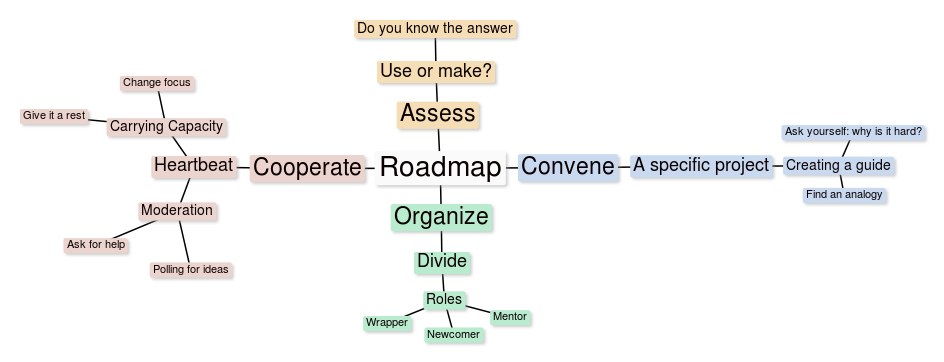
\includegraphics{images/pattern-language.jpg} {[}can this chart be
larger? Looks very small in text{]} The subsequent main sections of this
book -- \href{http://peeragogy.org/convene/}{\emph{Convene}},
\href{http://peeragogy.org/organize/}{\emph{Organize}},
\href{http://peeragogy.org/facilitate/}{\emph{Cooperate}} and
\href{http://peeragogy.org/assessment/}{\emph{Assess}} (for short) --
represent big clusters of patterns that are likely to come up time and
again in various projects.~ We can think of these as East, South, West,
and North in the diagram above. You are encouraged to invent your own
patterns and to connect them in new ways. You'll probably find quite a
few that we didn't include in the catalog. Each project has a unique
design, and it's own unique way in which things play out in practice.
What we've put together here is a starter kit. The peeragogy patterns
suggest a social way to do problem solving {[}3{]}, but once you get
used to the pattern concept you can use it to identify new problems no
one has ever thought of before, and that's even more powerful!

\hypertarget{references}{%
\subsubsection{References}\label{references}}

\begin{enumerate}
\def\labelenumi{\arabic{enumi}.}
\item
  Alexander, C., Ishikawa, S., and Silverstein, M. (1977). \emph{A
  Pattern Language: Towns, Buildings, and, Construction}, New York:
  Oxford University Press.
\item
  Gabriel, Richard P. (1996).
  \emph{\href{http://dreamsongs.net/Files/PatternsOfSoftware.pdf}{Patterns
  of Software}}, New York: Oxford University Press. (Includes a foreward
  by Christopher Alexander.)
\item
  Minsky, Marvin. (2008--2009). \emph{Essays on Education (for
  {O}{L}{P}{C})}, Massachusetts Institute of Technology Media Lab
  whitepaper,
  \href{http://web.media.mit.edu/~minsky/OLPC-1.html}{Available online.}
\end{enumerate}

%
\let\oldfootnote\footnote
\renewcommand*{\footnote}[1]{}%
\let\oldtextsuperscript\textsuperscript
\renewcommand*{\textsuperscript}[1]{}%
\chapter[\textbf{Patterns of Peeragogy}]{ Patterns of Peeragogy } \label{patterns}
\begin{refsection}

\begin{figure}
\begin{center}
\includegraphics[width=.9\textwidth,trim=0 30 10 2, clip=true]{../pictures/wisconsin-map.jpg}
\end{center}
\vspace{-.2cm}
\caption{A prototypical university.  Caption reads: ``Wisconsin State
  University, Madison, Wis. 1879''.  Inset captions describe the
  pictured buildings: ``Ladies Hall, South Dormitory, University Hall,
  Assembly Halls \& Library, North Dormitory, Science Hall, President's
  Residence, University Farm, and Washburn Observatory.''  Public
  domain.\label{madison-map}}
\end{figure}

This chapter outlines an approach to the organization of learning that draws on the principles of free\slash libre\slash open source software (FLOSS), free culture, and peer production.
Mako Hill suggests that one recipe for success in peer production is to take a familiar idea -- for example, an encyclopedia -- and make it easy for people to participate in building it \cite[Chapter 1]{mako-thesis}.  We will take hold of ``learning in institutions'' as a map (Figure \ref{madison-map}), although it does not fully conform to our chosen tacitly-familiar territory of \emph{peeragogy}.  To be clear, peeragogy is for \emph{any group of people who want to learn anything}.\footnote{\url{https://www.youtube.com/watch?v=TDRGJzoNbAc}}
 

Despite thinking about learning and adaptation that
may take place far outside of formal institutions, the historical
conception of a university helps give shape to our inqury.
%
The model university is not separate from the life of the state or its
citizenry, but aims to ``assume leadership in the application of
knowledge for the direct improvement of the life of the people in
every sphere'' \cite[p.~88]{curti1949university}. Research that
\emph{adds to the store of knowledge} is another fundamental
obligation of the university \cite[p.~550]{curti1949university}.
The university provides a familiar model for collaborative knowledge work
but it is not the only model available.
% wording issues here
Considering the role of collaboration in building Wikipedia,
StackExchange, and free\slash libre\slash open source software
development, we may be led to ask:  What might an accredited free\slash
libre\slash open university look like?  How would it compare or
contrast with the typical or stereotypical image of a university from
Figure \ref{madison-map}?  Would it have similar structural features, like a Library,
Dormitory, Science Hall and so on?  Would participants take
on familiar roles \cite{corneli+crowdsourcing}?  How would it compare
with historical efforts like the Tuskegee Institute that involved
students directly in the production of physical infrastructure
\cite{washington1986up,building-peeragogy-accelerator}?
%
We use the word \emph{peeragogy} to talk about collaboration in
relatively non-hierarchical settings.  Examples are found in
education, but also in business, government, volunteer, and NGO
settings.  Peeragogy involves both problem solving and problem
definition.  Indeed, in many cases it is preferable to focus on
solutions, since people know the ``problems'' all too well
\cite{ariyaratneXorganizationX1977}.  Participants in a peeragogical
endeavor collaboratively build emergent structures that are responsive
to their changing context, and that in turn, change that context. In
the Peeragogy project, we are developing the the theory and practice
of peeragogy.

\emph{Design patterns} offer a methodological framework that we have
used to clarify our focus and organize our work.  A design pattern
expresses a commonly-occurring problem, a solution to that problem,
and rationale for choosing this solution \cite{meszaros1998pattern}.
This skeleton is typically fleshed out with a \emph{pattern template}
that includes additional supporting material; individual patterns are
connected with each other in a \emph{pattern language}.  What we
present here is rather different from previous pattern languages that touch
on similar topics -- like \emph{Liberating Voices}
\cite{schuler2008liberating}, \emph{Pedagogical Patterns}
\cite{bergin2012pedagogical}, and \emph{Learning Patterns}
\cite{iba2014learning}.  At the level of the pattern template, our
innovation is simply to add a ``What's next'' annotation, which
anticipates the way the pattern will continue to ``resolve''.

% The patterns we introduce here focus on negotiating the execution and implementation of solutions in their practical context.
%  This often requires compromise, adjustments and even restarts.  

This addition mirrors the central considerations of our approach, which is all about human interaction, and the challenges, fluidity and unpredictability that come with it.  Something that works for one person may not work for another or may not even work for the same person in a slightly different situation.  We need to be ready to clarify and adjust what we do as we go.   Even so, it is hard to argue with a sensible-sounding formula like ``If W applies, do X to get Y.'' In our view, other pattern languages often achieve this sort of common sense rationality, and then stop.  Failure in the prescriptive model only begins when people try to define things more carefully and make context-specific changes -- when they actually try to put ideas into practice.  The problem lies in the inevitable distance between \emph{do as I say}, \emph{do as I do}, and \emph{do with me} \cite[p.~26]{deleuze1994difference}.
%One is put in mind of Alfred Korzybski's famous remark: ``the map is not the territory.''   
%% Indeed, the strong version of our claim is that peeragogy is needed in applications of any map, blueprint, or design that seeks to involve people as people.
%% In some idealized sense, according to a certain school of thought, ``control'' is all that's required to move from a well-thought-out design to successful execution.  But, where do the designs come from in the first place \cite{von2003cybernetics}?
%% %
%% Moreover, once they exist, designs need to be interpreted, and often, revised.  
If people are involved, things get messy.   They may think that they are on the same page, only to find out that their understandings are wildly different.  For  example, everyone may agree that the group needs to go ``that way.''  But how far?  How fast?  It is rare for a project to be able to set or even define all of the parameters accurately and concisely at the beginning.
And yet design becomes a ``living language'' \cite[p.~xvii]{alexander1977pattern}  just insofar as it is linked to action.  Many things have changed since Alexander suggested that ``you will get the most `power' over the language, and make it your own most effectively, if you write the changes in, at the appropriate places in the book'' \cite[p.~xl]{alexander1977pattern}.  We see more clearly what it means to inscribe the changing form of design not just in the margins of a book, or even a shared wiki, but in the lifeworld itself.  Other recent authors on patterns share similar views \cite{reiners2012approach, plast-project, schummer2014beyond}.


%% We use the patterns of peeragogy to
%% \emph{constitute and occupy practical or speculative problems as such}
%% \cite[p.~204]{deleuze1994difference}.
%% %
%% Our patterns are a living language just insofar as they are linked to
%% action.

% Till Sch{\"u}mmer \emph{et al.}~have emphasized that pattern authors ``talk about what by definition is tacit'' and highlight the role of nonverbal communication ``needed to communicate the unspeakable'' \cite[p.~9]{schummer2014beyond}.

%% Whereas existing projects like Wikimedia's Wikiversity\footnote{\url{https://www.wikiversity.org/}} and the Peer-2-Peer University (P2PU) have created ``a model for lifelong learning alongside traditional formal higher education,''\footnote{\url{https://www.p2pu.org/en/}} they stop well short of offering accredited degrees.  

Learning and collaboration are of interest to both organizational studies and computer science, where researchers are increasingly making use of social approaches to software design and development, as well as agent-based models of computation \cite{minsky1967programming,poetry-workshop}.
%
The design pattern community in particular is very familiar with practices that we think of as peeragogical, including shepherding, writers workshops, and design patterns themselves \cite{harrison1999language,coplien1997pattern,meszaros1998pattern}.  %% We hope to help design pattern authors and researchers expand on these strengths.

\subsection*{Pattern template}

%This section will give the reader a sense of how the paper is organized. 


%% \begin{wraptable}{r}{.52\textwidth}
%% {\small

%% \begin{tabular}{|p{.5\textwidth}|}
%% \hline
%% \emph{Motivation} for using this pattern.\\ \hline
%% \end{tabular}
%% \vspace{-.1cm}

%% \begin{tabular}{|p{.5\textwidth}|}
%% \hline
%% \emph{Context} of application.\\ \hline
%% \emph{Forces} that operate within the context of application, each with a mnemonic glyph. \\ \hline
%% \emph{Problem} the pattern addresses.\\ \hline
%% \emph{Solution} to the problem.\\ \hline
%% \emph{Rationale} for this solution.\\ \hline
%% \emph{Resolution} of the forces, named in bold.\\ \hline
%% \end{tabular}
%% \vspace{.1cm}

%% %% \begin{tabular}{|p{.5\textwidth}|}
%% %% \hline
%% %% \emph{Inversion} Problems that could arise, and when \emph{not} to use the pattern.\\ \hline
%% %% \end{tabular}
%% %% \vspace{.1cm}

%% \begin{tabular}{|p{.5\textwidth}|}
%% \hline
%% \emph{Example 1}: How the pattern manifests in current Wikimedia projects.\\ \hline
%% \emph{Example 2}: How the pattern could inform the design of a future university.\\ \hline
%% \end{tabular}
%% \vspace{.1cm}

%% \begin{tabular}{|p{.5\textwidth}|}
%% \hline
%% \emph{What's Next in the Peeragogy Project}: How the pattern relates to our collective intention in the Peeragogy project\\ \hline
%% \end{tabular}

%% \vspace{-.1cm}
%% \caption{Pattern template.\label{tab:pattern-template}}
%% \vspace{-.9cm}
%% }
%% \end{wraptable}

Table \ref{tab:pattern-template} shows the pattern template that we use to present our patterns.
Along with the traditional design patterns components \cite{meszaros1998pattern}, each of our patterns is fleshed out with two illustrative examples.  The first is descriptive, and looks at how the pattern applies in current Wikimedia projects.  We selected Wikimedia as a source of examples because the project is familiar, a demonstrated success, and readily accessible.  The second example shows how the pattern could be applied in the design of a future university.  Each pattern concludes with a boxed annotation: ``\emph{What's Next in the Peeragogy Project}''.

%% Section \ref{sec:Peeragogy} defines the concept of \patternname{Peeragogy} more explicitly the form of a design pattern.  Sections \ref{sec:Roadmap}--\ref{sec:Scrapbook} present the other patterns in our pattern language. Figure \ref{fig:connections} illustrates their interconnections. Table \ref{tab:core} summarizes the ``nuts and bolts'' of the pattern language.
%% Section \ref{sec:Distributed_Roadmap} collects our ``What's Next'' steps, summarizes the outlook of the Peeragogy project.

%OSS: who cares? start w/example?
\subsection*{A short motivating example}
When one relative \patternname{Newcomer} was still in the onboarding
process in Peeragogy project, she hit a wall in understanding the
``patterns'' section in the \emph{Peeragogy Handbook} v1.  A more
seasoned peer invited her to a series of separate discussions with
their own \patternname{Heartbeat} to flesh out the patterns and make
them more accessible.  At that time the list of patterns was simply a
list of paragraphs describing recurrent trends.  During those
sessions, the impact and meaning of patterns captured her imagination.
She went on to become the champion for the pattern language and its
application in the Peeragogy project.  During a ``hive editing''
session, she proposed the template we initially used to give structure
to the patterns.  She helped further revise the pattern language for
the \emph{Peeragogy Handbook} v3, and attended PLoP 2015.  While a new
domain can easily be overwhelming, this newcomer found \patternname{A
  specific project} to start with, and scaffolded her knowledge and
contributions from that foundation.

\begin{table}
{\centering
\vspace{-.65cm}
\begin{tabular}{|p{.5\textwidth}|}
\hline
\emph{Motivation} for using this pattern.\\ \hline
\end{tabular}
\vspace{.1cm}

\begin{tabular}{|p{.5\textwidth}|}
\hline
\emph{Context} of application.\\ \hline
\emph{Forces} that operate within the context of application, each with a mnemonic glyph. \\ \hline
\emph{Problem} the pattern addresses.\\ \hline
\emph{Solution} to the problem.\\ \hline
\emph{Rationale} for this solution.\\ \hline
\emph{Resolution} of the forces, named in bold.\\ \hline
\end{tabular}
\vspace{.1cm}

%% \begin{tabular}{|p{.5\textwidth}|}
%% \hline
%% \emph{Inversion} Problems that could arise, and when \emph{not} to use the pattern.\\ \hline
%% \end{tabular}
%% \vspace{.1cm}

\begin{tabular}{|p{.5\textwidth}|}
\hline
\emph{Example 1}: How the pattern manifests in current Wikimedia projects.\\ \hline
\emph{Example 2}: How the pattern could inform the design of a future university.\\ \hline
\end{tabular}
\vspace{.1cm}

\begin{tabular}{|p{.5\textwidth}|}
\hline
\emph{What's Next in the Peeragogy Project}: How the pattern relates to our collective intention in the Peeragogy project\\ \hline
\end{tabular}

\par}
\vspace{-.1cm}
\caption{Pattern template.\label{tab:pattern-template}}
\vspace{-.9cm}
\end{table}

\FloatBarrier

\begin{figure}
\vspace{-.9in}
{\centering
\begin{tikzpicture}[dot/.style={circle,inner sep=1pt,fill,name=#1},nodes = {align=center}]
\node (headline) at (5,10.75) {\large \emph{Connections between the patterns of peeragogy}};
%\draw[step=1cm,gray,very thin] (0,0) grid (10,10);
\node (assess) at (5, 10) {{\Large {\sc Assess}}};
\node (organize) at (5, -2.75) {{\Large {\sc Organize}}};
\node (cooperate)[text width=2cm,align=center,rotate=270] at (10, 5) {{\Large {\sc Convene}}};
\node (convene)[text width=15cm,align=center,rotate=90] at (-.25, 5) {{\Large {\sc Cooperate}}};
%%%%%%%%%%%%%%%%%%%%%%%%%%%%%%%%%%%%%%%%%%%%%%%%%%%%%%%%%%%%%%%%%%%%%%%%%%%%%%%%%%%%%%%%%%%%%%%%%%%%%
\node[below = 5cm of assess] (roadmap) {\hyperref[sec:Roadmap]{\emph{Roadmap}}\\(p.~\pageref{sec:Roadmap})};
\node (reduce) at (5, 8.75) {\hyperref[sec:Reduce, reuse, recycle]{\emph{Reduce, reuse, recycle}}\\(p.~\pageref{sec:Reduce, reuse, recycle})};
\node (carryingcapacity) at (1.25, 7.15) {\hyperref[sec:Carrying capacity]{\emph{Carrying capacity}}\\(p.~\pageref{sec:Carrying capacity})};
\node[below = 3.2cm of carryingcapacity] (heartbeat) {\hyperref[sec:Heartbeat]{\emph{Heartbeat}}\\(p.~\pageref{sec:Heartbeat})};
\node (aspecificproject) at (8.5, 6.5) {\hyperref[sec:A specific project]{\emph{A specific project}}\\(p.~\pageref{sec:A specific project})};
\node[below = 1.5cm of roadmap] (wrapper) {\hyperref[sec:Wrapper]{\emph{Wrapper}}\\(p.~\pageref{sec:Wrapper})};
\node (newcomer) at (8.5, 3) {\hyperref[sec:Newcomer]{\emph{Newcomer}}\\(p.~\pageref{sec:Newcomer})};
\node[below = 1.7cm of wrapper] (scrapbook) {\hyperref[sec:Scrapbook]{\emph{Scrapbook}}\\(p.~\pageref{sec:Scrapbook})};
\node[above = 1cm of aspecificproject] (peeragogyproject) {\hyperref[sec:Peeragogy]{\emph{Peeragogy}}\\(p.~\pageref{sec:Peeragogy})};
%%%%%%%%%%%%%%%%%%%%%%%%%%%%%%%%%%%%%%%%%%%%%%%%%%%%%%%%%%%%%%%%%%%%%%%%%%%%%%%%%%%%%%%%%%%%%%%%%%%%%
\draw[-{Latex[width=2mm]},draw=black] (peeragogyproject) -- (aspecificproject);
% \draw[-{Latex[width=2mm]},draw=black] (aspecificproject) -- (par);
\draw[-{Latex[width=2mm]},draw=black] (aspecificproject) -- (roadmap);
\draw[-{Latex[width=2mm]},draw=black] (aspecificproject.235) to[out=235,in=40] (scrapbook);
\draw[-{Latex[width=2mm]},draw=black] (aspecificproject) -- (carryingcapacity);
\draw[-{Latex[width=2mm]},draw=black] (carryingcapacity.337) -- (newcomer);
\draw[-{Latex[width=2mm]},draw=black] (carryingcapacity.330) -- (roadmap);
\draw[-{Latex[width=2mm]},draw=black] (carryingcapacity.5) to[out=5,in=200] (peeragogyproject);
\draw[-{Latex[width=2mm]},draw=black] ([xshift=1mm]carryingcapacity.south) -- (scrapbook.140);
% \draw[-{Latex[width=2mm]},draw=black] ([xshift=2mm]creatingaguide.160) to[out=-215,in=-67] (carryingcapacity);
\draw[-{Latex[width=2mm]},draw=black] (heartbeat) -- (aspecificproject.185);
\draw[-{Latex[width=2mm]},draw=black] (heartbeat) -- (carryingcapacity);
\draw[-{Latex[width=2mm]},draw=black] (heartbeat) -- (scrapbook.155);
\draw[-{Latex[width=2mm]},draw=black] (heartbeat) -- (reduce.215);
\draw[-{Latex[width=2mm]},draw=black] (newcomer) -- ([xshift=4mm]reduce.south);
\draw[-{Latex[width=2mm]},draw=black] (newcomer) -- (aspecificproject);
% \draw[-{Latex[width=2mm]},draw=black] (newcomer) -- (creatingaguide.north);
\draw[-{Latex[width=2mm]},draw=black] (newcomer) -- (roadmap);
% \draw[-{Latex[width=2mm]},draw=black] (par) -- (scrapbook);
\draw[-{Latex[width=2mm]},draw=black] (roadmap) -- (peeragogyproject.215);
\draw[-{Latex[width=2mm]},draw=black] (roadmap) -- (newcomer);
\draw[-{Latex[width=2mm]},draw=black] (roadmap) -- (wrapper);
\draw[-{Latex[width=2mm]},draw=black] (roadmap) -- (heartbeat);
\draw[-{Latex[width=2mm]},draw=black] (roadmap) -- (aspecificproject);
% \draw[-{Latex[width=2mm]},draw=black] (scrapbook) -- (par);
\draw[-{Latex[width=2mm]},draw=black] (scrapbook) -- (wrapper);
\draw[-{Latex[width=2mm]},draw=black] (scrapbook.110) to[out=120,in=250] (reduce.245);
\draw[-{Latex[width=2mm]},draw=black] (scrapbook.70) to[out=45,in=305] (roadmap.325);
% \draw[-{Latex[width=2mm]},draw=black] ([xshift=2mm,yshift=-.4mm]reduce.south) -- (creatingaguide);
\draw[-{Latex[width=2mm]},draw=black] ([xshift=4mm]reduce.200) -- (carryingcapacity);
\draw[-{Latex[width=2mm]},draw=black] (reduce) -- (roadmap);
\draw[-{Latex[width=2mm]},draw=black] (wrapper.175) -- (heartbeat);
\draw[-{Latex[width=2mm]},draw=black] ([xshift=-.5mm]wrapper.360) -- (newcomer);
\draw[-{Latex[width=2mm]},draw=black] (wrapper) -- ([xshift=2.3mm]carryingcapacity.south);
\draw[-{Latex[width=2mm]},draw=black] (wrapper) -- (roadmap);
\end{tikzpicture}


\par
}

\caption{Connections between the patterns of peeragogy.  An arrow points from pattern \textbf{A} to pattern \textbf{B} if the text of the description of pattern \textbf{A} references pattern \textbf{B}.  Labels at the borders of the figure correspond to the main sections of the \emph{Peeragogy Handbook}.\label{fig:connections}}
\end{figure}

\FloatBarrier

\begin{table}
{\footnotesize
\newcolumntype{C}{>{\centering\arraybackslash}X}
\begin{tabularx}{\textwidth}{|C|}
\hline
%\rule{\textwidth}{0mm}
\vspace{-.4em}\cellcolor{Gray!30} \color{Black} 1. \patternnameext{Peeragogy}\vspace{.25em}\\
\hline
\vspace{.01em}
\textbf{How can we find solutions together?}\\
Get concrete about what the real problems are.
\vspace{.4em}\\
\hline 
%%%%%%%%%%%%%%%%%%%%
\vspace{-.4em}\cellcolor{Gray!30} \color{Black} 2. \patternnameext{Roadmap}\vspace{.4em}\\
\hline
\vspace{.01em}
\textbf{How can we get everyone on the same page?}\\
Build a plan that we keep updating as we go along.
\vspace{.4em}\\
\hline
%%%%%%%%%%%%%%%%%%%%
\vspace{-.4em}\cellcolor{Gray!30} \color{Black} 3. \patternnameext{Reduce, reuse, recycle}\vspace{.4em}\\
\hline
\vspace{.01em}
\textbf{How can we avoid undue isolation?}\\
Use what's there and share what we make.
\vspace{.4em}\\
\hline
%%%%%%%%%%%%%%%%%%%%
\vspace{-.4em}\cellcolor{Gray!30} \color{Black} 4. \patternnameext{Carrying capacity}\vspace{.4em}\\
\hline
\vspace{.01em}
\textbf{How can we avoid becoming overwhelmed?}\\
Clearly express when we're frustrated.
\vspace{.4em}\\
\hline
%%%%%%%%%%%%%%%%%%%%
\vspace{-.4em}\cellcolor{Gray!30} \color{Black} 5. \patternnameext{A specific project}\vspace{.4em}\\
\hline
\vspace{.01em}
\textbf{How can we avoid becoming perplexed?}\\
Focus on concrete, doable tasks.
\vspace{.4em}\\
\hline
%%%%%%%%%%%%%%%%%%%%
\vspace{-.4em}\cellcolor{Gray!30} \color{Black} 6. \patternnameext{Wrapper}\vspace{.4em}\\
\hline
\vspace{.01em}
\textbf{How can people stay in touch with the project?}\\
Maintain a summary of activities and any adjustments to the plan.
\vspace{.4em}\\
\hline
%%%%%%%%%%%%%%%%%%%%
\vspace{-.4em}\cellcolor{Gray!30} \color{Black} 7. \patternnameext{Heartbeat}\vspace{.4em}\\
\hline
\vspace{.01em}
\textbf{How can we make the project ``real'' for participants?}\\
Keep up a regular, sustaining rhythm.
\vspace{.4em}\\
\hline
%%%%%%%%%%%%%%%%%%%%
\vspace{-.4em}\cellcolor{Gray!30} \color{Black} 8. \patternnameext{Newcomer}\vspace{.4em}\\
\hline
\vspace{.01em}
\textbf{How can we make the project accessible to new people?}\\
Let's learn together with newcomers.
\vspace{.4em}\\
\hline
%%%%%%%%%%%%%%%%%%%%
\vspace{-.4em}\cellcolor{Gray!30} \color{Black} 9. \patternnameext{Scrapbook}\vspace{.4em}\\
\hline
\vspace{.01em}
\textbf{How can we maintain focus as time goes by?}\\
Move things that are not of immediate use out of focus.
\vspace{.4em}\\
\hline
\end{tabularx}
}
\smallskip
\caption{An overview of the problems and solutions in our pattern language.\label{tab:core}}
\end{table}

\FloatBarrier


% deferring a more detailed elaboration of next steps in the educational arena to future work that will build on this basis.
% Technology has come a long way since Alexander suggested ``you will get the most `power' over the language, and make it your own most effectively, if you write the changes in, at the appropriate places in the book'' \cite[p.~xl]{alexander1977pattern}.
% While Christian Kohls insightfully describes patterns as the unique resolution of the dynamical forces acting in a given context \cite{kohls2010structure,kohls2011structure}.
%%% Patterns come to you through mindful awareness ... Charlotte: I think about patterns all the time now, I think about what makes me productive in a team.
% So, while we speak the same language as other developers of design patterns, our orientation is somewhat different, and our understanding of the word `pattern' is nuanced because we aim to take full account of the lifecycle of patterns.  Our work contributes to a recent ``performative'' turn \cite{schummer2014beyond}, which we believe gets at the heart of what design patterns can do.
%  
% In practical terms, we believe the patterns that we introduce here will be useful for students and educators who want their work to have real-world relevance, to activists and policy-makers who want to develop practicable solutions to large-scale problems, and to employees and managers who, like it or not, find themselves working in distributed teams. 

\printbibliography[heading=subbibliography]
\end{refsection}

\newpage
 \label{sec:Introduction}
%
\section{Peeragogy} \label{sec:Peeragogy}
\hypertarget{peeragogy}{%
\subsection{Peeragogy}\label{peeragogy}}

\hypertarget{motivation}{%
\subsubsection{Motivation}\label{motivation}}

This pattern is relevant to anyone who wants to do active learning
together with others in a relatively non-hierarchical setting.

\hypertarget{context}{%
\subsubsection{Context}\label{context}}

Collaborative projects like Wikipedia, StackExchange, and FLOSS
represent an implicit challenge to the old ``industrial'' organization
of work. This new way of working appears to promise something more
resilient, more exciting, and more humane. The rhetoric has been
questioned {{[}3,9{]}}. In and across these ``free'', ``open'',
post-modern organizations, individual participants are learning
{{[}7{]}} -- and that they collectively change the methods and
infrastructure as they go. Because everyone in these projects primarily
learns by putting in effort on a shared work-in-progress, participants
are more in touch with an \emph{equality of intelligence} than an
\emph{inequality of knowledge} {{[}4:38, 119{]}}. At the same time, they
invoke a form of friendly competition, in which \emph{the best
craftmanship wins} {{[}5:89{]}}.

\hypertarget{forces}{%
\subsubsection{Forces}\label{forces}}

\begin{quote}

\includegraphics{images/threshold.png} \textbf{Threshold}: inclusiveness
and specificity are in tension.\\

\includegraphics{images/trust.png} \textbf{Trust}: is only built through
sharing and reciprocity.
\end{quote}

\hypertarget{problem}{%
\subsubsection{Problem}\label{problem}}

Even a highly successful project like Wikipedia is a work in progress
that can be improved to \emph{better} empower and engage people around
the world, to develop \emph{richer and more useful} educational content,
and to disseminate it \emph{more} effectively -- and deploy it more
creatively.\footnote{\url{https://wikimediafoundation.org/wiki/Mission_statement}}
How to go about this is a difficult question, and we don't know the
answers in advance. There are rigorous challenges facing smaller
projects as well, and fewer resources to draw on. Many successful free
software projects are not particularly collaborative -- and the largest
projects are edited only by a small minority of users {{[}2,10{]}}. Can
we work smarter together?

\hypertarget{solution}{%
\subsubsection{Solution}\label{solution}}

The act of asking ``can we work smarter together?'' puts learning front
and center. Peeragogy takes that ``center'' and distributes it across a
pool of heterogeneous relationships. Indeed, peeragogy can be understood
as an up-to-date revision of Alexander's {{Network of Learning}}
{{[}1:99{]}}. It \emph{decentralizes the process of learning and
enriches it through contact with many places and people} in
interconnected networks that may reach all over the world. Importantly,
while people involved in a peeragogical process may be collaborating on
{{A specific project}}, they don't have to be direct collaborators
outside of the learning context or co-located in time or space. Just as
theories and practices of pedagogy articulate the transmission of
knowledge from teachers to students, peeragogy articulates the way peers
produce and use knowledge together (Figure {[}fig:connections{]}).

\hypertarget{rationale}{%
\subsubsection{Rationale}\label{rationale}}

The peeragogical approach particularly addresses the problems of small
projects stuck in their individual silos, and large projects becoming
overwhelmed by their own complexity. It does this by going the opposite
route: explicating \emph{what by definition is tacit} and employing
\emph{a continuous design process} {{[}8:9--10{]}}. As Howard Rheingold
remarks in the foreword to the \emph{Peeragogy Handbook}: ``What made
this work? Polycentric leadership is one key'' {{[}6:iii{]}}.
``Peer-led'' shouldn't suggest that there are no leaders: rather, it
means that multiple leaders act as peers.

\hypertarget{resolution}{%
\subsubsection{Resolution}\label{resolution}}

Peeragogy helps people in different projects describe and solve real
problems. If you share the problems that you're experiencing with
others, there's a reasonable chance that someone may be able to help you
solve them. Bringing a problem across the \textbf{threshold} of someone
else's awareness helps achieve clarity. This process can guide
individual action in ways that we wouldn't have seen on our own, and may
lead to new forms of collective action we would never have imagined
possible. People who gain experience comprehending problems together
build \textbf{trust}. Making room for multiple right answers contributes
further to resolving the tension between generality and specificity.

\hypertarget{example-1}{%
\subsubsection{Example 1}\label{example-1}}

Wikipedia and its sister sites Wiktionary, Wikiversity, etc.
(collectively ``Wikimedia'') rely on user-generated content, peer
produced software, and are managed, by and large, by a pool of users who
choose to get involved with governance and other ``meta''
duties.\footnote{\url{https://www.wikimedia.org/}} The Wikimedia
Foundation maintains the servers and acts on behalf of this ``global
movement''. They achieve something quite impressive: Wikipedia is the
7th most popular website in the world, but the Wikimedia Foundation has
under 300 employees. For comparison, the 6th (Amazon) and 8th (QQ) most
popular websites are run by companies with over 200K and 28K employees,
respectively.\footnote{\url{https://en.wikipedia.org/wiki/Wikimedia_Foundation\#Employees}},\footnote{\url{http://phx.corporate-ir.net/phoenix.zhtml?c=97664\&p=irol-newsArticle\&ID=2100418}},\footnote{\url{https://www.google.com/finance?cid=695431}},\footnote{\url{http://www.alexa.com/topsites}}

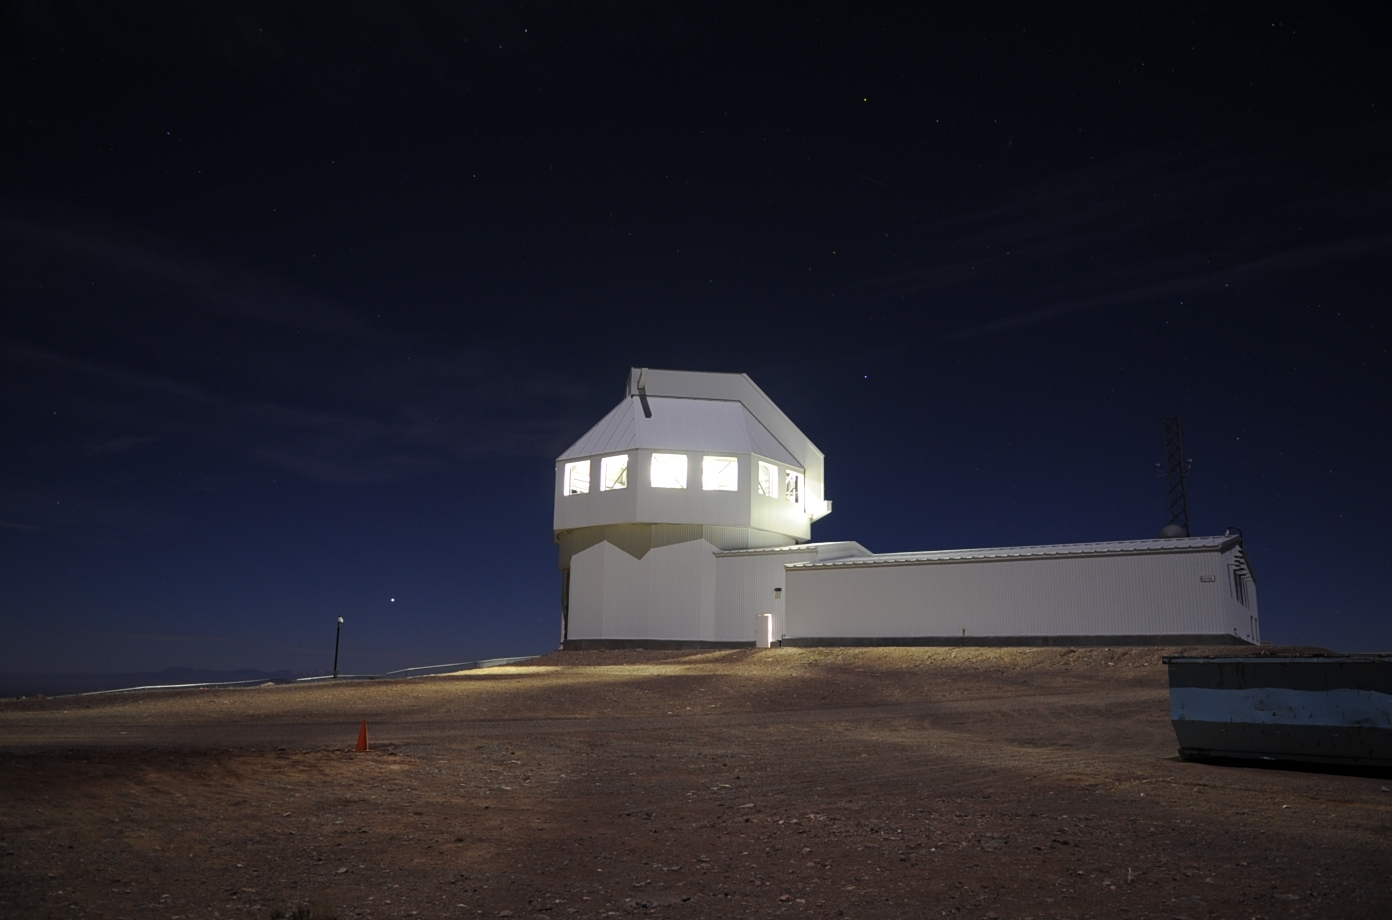
\includegraphics{images/Space_Surveillance_Telescope.jpg}
\emph{Observatory : Space Surveillance Telescope, New Mexico.}

\hypertarget{example-2}{%
\subsubsection{Example 2}\label{example-2}}

Although one of the strengths of {{Peeragogy}} is to distribute the
workload, this does not mean that infrastructure is irrelevant. The
students and researchers of the future university will need access to an
Observatory and other scientific apparatus if they are to reach \emph{ad
astra, per aspera} (Figure 1).\footnote{Latin: ``With difficulty, to the
  stars.''}

\hypertarget{whats-next-in-the-peeragogy-project}{%
\subsubsection{What's Next in the Peeragogy
Project*}\label{whats-next-in-the-peeragogy-project}}

We intend to revise and extend the \emph{Patterns of Peeragogy} into a
framework that can describe and scaffold the learning that happens
inside and outside of institutions.

\hypertarget{references}{%
\subsubsection{References}\label{references}}

\begin{enumerate}
\def\labelenumi{\arabic{enumi}.}
\item
  Christopher Alexander, Sara Ishikawa, and Murray Silverstein. 1977.
  \emph{A Pattern Language: Towns, Buildings, Construction}. Oxford
  University Press, Oxford.
\item
  Benjamin Mako Hill. 2011. When Free Software Isn't (Practically)
  Better. Retrieved from
  \url{http://www.gnu.org/philosophy/when_free_software_isnt_practically_better.html}
\item
  Daniel Kreiss, Megan Finn, and Fred Turner. 2011. The limits of peer
  production: Some reminders from Max Weber for the network society.
  \emph{New Media \& Society} 13, 2: 243--259.
\item
  Jacques Rancière. {[}1987{]} 1991. \emph{The ignorant schoolmaster:
  Five lessons in intellectual emancipation}. Stanford University Press.
\item
  Eric S Raymond. 2001. \emph{The Cathedral \& the Bazaar: Musings on
  Linux and open source by an accidental revolutionary}. O'Reilly Media,
  Inc.
\item
  H. Rheingold and others. 2015. \emph{The Peeragogy Handbook}.
  PubDomEd/Pierce Press, Chicago, IL./Somerville, MA. Retrieved from
  \url{http://peeragogy.org}
\item
  J. P. Schmidt. 2009. Commons-Based Peer Production and education.
  \emph{Free Culture Research Workshop, Harvard University}: 1--3.
  Retrieved from
  \url{http://cyber.law.harvard.edu/fcrw/sites/fcrw/images/Schmidt_Education_FreeCulture_25Oct2009.pdf}
\item
  Till Schümmer, Joerg M Haake, and Wolfgang Stark. 2014. Beyond
  rational design patterns. \emph{Proceedings of the 19th european
  conference on pattern languages of programs}, ACM, 13 pp.
\item
  Aaron Shaw and Benjamin Mako Hill. 2014. Laboratories of Oligarchy?:
  How the iron law extends to peer production. \emph{Journal of
  Communication} 64, 2: 215--238.
\item
  Aaron Swartz. 2006. Who Writes Wikipedia? Retrieved from
  \url{http://www.aaronsw.com/weblog/whowriteswikipedia}
\end{enumerate}

\begin{center}\rule{0.5\linewidth}{0.5pt}\end{center}

\hypertarget{notes}{%
\subsubsection{Notes}\label{notes}}

%
\section{Roadmap} \label{sec:Roadmap}
\hypertarget{roadmap}{%
\subsection{Roadmap}\label{roadmap}}

\hypertarget{motivation}{%
\subsection{Motivation}\label{motivation}}

This pattern shows how your group can define the scope of their project
and make a realistic plan to address it. This pattern provides the
backbone of our pattern language. It can be used to find a shared goal.

\hypertarget{context}{%
\subsection{Context}\label{context}}

\href{http://peeragogy.github.io/pattern-peeragogy.html}{Peeragogy} has
both distributed and centralized aspects. The discussants or
contributors who collaborate on a project have different points of view
and heterogeneous priorities, but they come together in conversations
and joint activities.

\hypertarget{forces}{%
\subsection{Forces}\label{forces}}

\begin{quote}
\Svariety\ \textbf{Variety}: people have different goals and interests in mind.\\
\Sclarity\ \textbf{Clarity}: some goals may be quite specific, and some rather vague.\\
\Scoherence\ \textbf{Coherence}: only some of these goals will be well-aligned.
\end{quote}

\hypertarget{problem}{%
\subsection{Problem}\label{problem}}

In order to collaborate, people need a way to share current, though
incomplete, understanding of the space they are working in, and to
nurture relationships with one another and the other elements of this
space. At the outset, there may not even be a coherent vision for a
project -- but a only loose collection of motivations and sentiments.
Once the project is up and running, people are likely to pull in
different directions.

\hypertarget{solution}{%
\subsection{Solution}\label{solution}}

Building a guide to the goals, activities, experiments and working
methods can help {{Newcomers}} and old-timers alike understand their
relationship with the project. It may combine features of a manifesto, a
syllabus, and an issue tracker. It may be a design pattern or a pattern
language {{[}3{]}}. The distinguishing qualities of a project Roadmap
are that it should be adaptive to circumstances, and that it should
ultimately get us from \emph{here} to \emph{there}. By this same token,
any given version of the roadmap is seen as fallible. In lieu of
widespread participation, the project's {{Wrapper}} should attempt to
synthesize an accurate roadmap that is informed by participants'
behavior, and should help moderate in case of conflict. Nevertheless,
full consensus is not necessary: different goals, with different
\emph{heres} and \emph{theres}, can be pursued separately, while
maintaining communication.

\hypertarget{rationale}{%
\subsection{Rationale}\label{rationale}}

The group evolves from a less-sophisticated to a more-sophisticated
manner of operating by using the roadmap. Using the roadmap builds a
collective awareness of how things are working in practice. In the
Peeragogy project our initial roadmap was a ``crowdsourced'' outline of
the first edition of the \emph{Peeragogy Handbook}. Later, it took the
form of a schedule of meetings following a regular {{Heartbeat}},
supplemented by a list of upcoming deadlines. Most recently, our roadmap
is expressed in the emergent objectives collected at the end of current
paper. We have seen that a list of nice-to-have features created in a
top-down fashion is comparatively unlikely to go anywhere! A backlog of
tasks and a realistic plan for accomplishing them are vastly different
things. An adaptive roadmap is an antidote to {{Tunnel Vision}}
{{[}1{]}}.

\hypertarget{resolution}{%
\subsection{Resolution}\label{resolution}}

An emergent roadmap is rooted in real problems and justifiable
solutions-in-progress in all their \textbf{variety} and communicates
both resolution and follow-through. The process of meshing varied issues
with one another requires thought and discussion, and this encourages
\textbf{clarity}. The test of \textbf{coherence} is that contributed
goals and ideas should be actionable. The ultimate quality-control test
is if it worked, i.e., did it come to pass that the task(s) the roadmap
was created to achieve ended up being achieved? If all of the issues
that the roadmap outlines are not resolved, the roadmap itself should be
revised. Without a roadmap, we would never know.

\hypertarget{example-1}{%
\subsection{Example 1}\label{example-1}}

The \emph{Help} link present on every Wikipedia page could be seen as a
localized {{Roadmap}} for individual user engagement: it tells users
what they can do with the site, and gives instructions on how to do
it.\footnote{\url{https://en.wikipedia.org/wiki/Help:Contents}} someone
who knows what they're doing, there are around 30 pages listing articles
with various kinds of problems, for example articles tagged with style
issues, or ``orphaned'' articles (i.e., articles with no links from
other pages in the encyclopedia).\footnote{\url{https://en.wikipedia.org/wiki/Category:Wikipedia_article_cleanup}},\footnote{\url{https://en.wikipedia.org/wiki/Category:Wikipedia_articles_with_style_issues}},\footnote{\url{https://en.wikipedia.org/wiki/Category:All_orphaned_articles}}
In 2010-2011, Wikimedia developed a strategic plan drawing on community
input {{[}2{]}}. In 2015, a two-week Community Consultation was carried
out; synthesis resulted in ``a direction that will guide the decisions
for the organization.''\footnote{\url{https://blog.wikimedia.org/2015/02/23/strategy-consultation/}}
Community-organized WikiProjects often invite and guide involvement on
{{A specific project}}.

\hypertarget{example-2}{%
\subsection{Example 2}\label{example-2}}

In a future university run in a peer produced manner, a fancy
President's Residence presumably wouldn't be needed. Leadership would be
carried out in a more collaborative and distributed fashion. However,
depending on just how distributed things are, it may turn out to be
useful for project facilitators to gather at a University Hall. Whereas
there is strength in numbers, there is leverage in organization. This is
what the {{Roadmap}} provides.

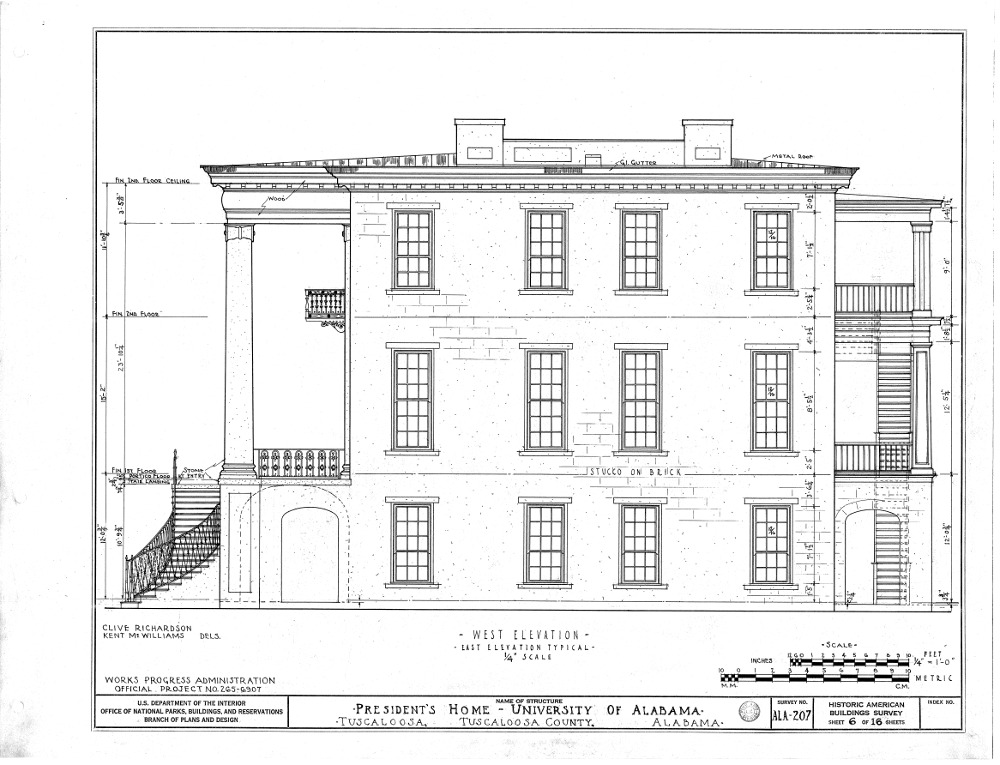
\includegraphics{images/alabama-small.jpg}\\
\emph{President's Residence, University of Alabama.}

\hypertarget{whats-next-in-the-peeragogy-project}{%
\subsection{What's Next in the Peeragogy
Project}\label{whats-next-in-the-peeragogy-project}}

If it becomes clear that something needs to change about the project,
that is a clue that we might need to revise our patterns or record a new
one. We can use the names of the patterns to tag our upcoming tasks.

\hypertarget{references}{%
\subsection{References}\label{references}}

\begin{enumerate}
\def\labelenumi{\arabic{enumi}.}
\item
  David M. Dikel, David Kane, and James R. Wilson. 2001. \emph{Software
  architecture: Organizational principles and patterns}. Pearson
  Education.
\item
  Eugene Eric Kim and others. 2011. \emph{Wikimedia Strategic Plan: A
  collaborative vision for the movement through 2015}. Wikimedia
  Foundation.
\item
  Christian Kohls. 2010. The structure of patterns. \emph{Proceedings of
  the 17th Conference on Pattern Languages of Programs}, ACM, 12.
\end{enumerate}

\begin{center}\rule{0.5\linewidth}{0.5pt}\end{center}

%
\section{Reduce, reuse, recycle} \label{sec:Reduce, reuse, recycle}
\hypertarget{reduce-reuse-recycle}{%
\subsection{Reduce, reuse, recycle}\label{reduce-reuse-recycle}}

\hypertarget{motivation}{%
\subsection{Motivation}\label{motivation}}

This pattern can guide project participants in identifying and managing
available resources.

\hypertarget{context}{%
\subsection{Context}\label{context}}

In a peer production context, you are simultaneously ``making stuff''
and building on the work of others.

\hypertarget{forces}{%
\subsection{Forces}\label{forces}}

\begin{quote}
\Sderivative\ \textbf{Derivative}: you don't have to do everything yourself!\\
\Ssensemaking\ \textbf{Sensemaking}: resources are useful only when you can make sense of them.\\
\Ssharing\ \textbf{Sharing}: your understanding gains robustness when you share with others.
\end{quote}

\hypertarget{problem}{%
\subsection{Problem}\label{problem}}

Many projects die because the cost of
{{\href{http://c2.com/cgi/wiki?ReinventingTheWheel}{Reinventing the
Wheel}}} {[}c2{]} is too high. However, this is just one possible
symptom of overfocus on a few priorities. Concerns may also arise if the
project's output is not actually used by anyone.

\hypertarget{solution}{%
\subsection{Solution}\label{solution}}

``Steal like an artist,'' and make it possible for other people to build
on your work too. In the Peeragogy project, we have used off-the-shelf
and hosted software suited to the task at hand (including: Drupal,
Google+, Google Hangouts, Google Docs, Wordpress, pandoc, Github,
ShareLaTeX). Early on we agreed to release our \emph{Peeragogy Handbook}
under the terms of the Creative Commons Public Domain Dedication (CC0),
the legal instrument that grants the greatest possible leeway to
downstream users.\footnote{\url{https://creativecommons.org/publicdomain/zero/1.0/}}
This has allowed us and others to repurpose and improve its contents in
other settings, including the current paper. Follow the steps indicated
by the keywords in the pattern's title:

\begin{itemize}
\tightlist
\item
  \emph{Reduce} the panoply of interesting interrelated ideas and
  methods to a functional core (e.g.~writing a book).
\item
  \emph{Reuse} resources relevant to this aim, factoring in ``things I
  was going to have to do anyway'' from everyone involved.
\item
  \emph{Recycle} what you've created in new connections and
  relationships.
\end{itemize}

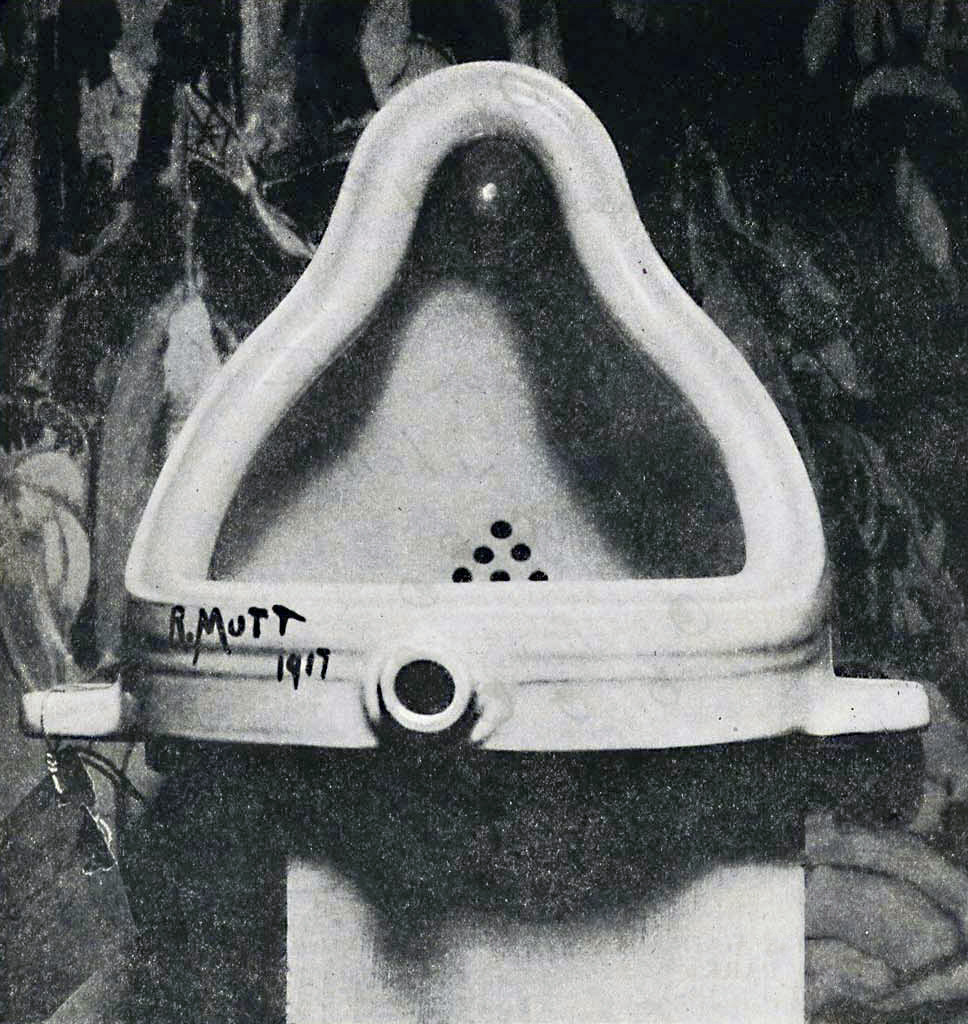
\includegraphics{images/Duchamp_Fountaine.jpg}\\
\emph{A paradigmatic example of found-art. ``Fountain by R. Mutt,
Photograph by Alfred Stieglitz, THE EXHIBIT REFUSED BY THE
INDEPENDENTS''.}

\hypertarget{rationale}{%
\subsection{Rationale}\label{rationale}}

Clearly we are not the first people to notice the problems with
wheel-reinvention, including ``missing opportunities, repeating common
mistakes, and working harder than we need to.''\footnote{\url{https://blog.wikimedia.org/2013/11/19/learning-patterns-new-way-share-important-lessons/}}
As a guest in one of our hangouts, Willow Brugh, of Geeks without Bounds
and the MIT Media Lab, remarked that \emph{people often think that they
need to build a community, and so fail to recognize that they are
already part of a community.}\footnote{\url{https://www.youtube.com/watch?v=NpyQfYVKfBI}}
converted our old pattern catalog from the \emph{Peeragogy Handbook}
into this paper, sharing it with a new community and gaining new
perspectives; could we do something similar again?

\hypertarget{resolution}{%
\subsection{Resolution}\label{resolution}}

Reweaving old material into \textbf{derivative} designs and new material
into existing frameworks, we build deeper understanding, and carry out
collective \textbf{sensemaking}. The project's {{Roadmap}} develops by
making sense of existing resources -- including our worries and
concerns. Often we only know what these are when we attempt to
\textbf{share} them. Drawing on a wide range of resources boosts our
collective {{Carrying capacity}}.

\hypertarget{example-1}{%
\subsection{Example 1}\label{example-1}}

Contributors are encouraged to recycle existing works that are
compatible with the Wikimedia-wide Creative Commons
Attribution-ShareAlike (CC-By-SA) license.\footnote{\url{https://creativecommons.org/weblog/entry/15411/}}
Some sub-projects have been created purely to help repurpose other
existing works in this way.\footnote{\url{https://en.wikipedia.org/wiki/Wikipedia:WikiProject_Mathematics/PlanetMath_Exchange}}
On the downstream side, DBPedia is an important resource for the
semantic web, built by collating data from Wikipedia's
``infoboxes.''\footnote{\url{http://wiki.dbpedia.org/}} themselves
increasingly being populated automatically using information from
WikiData.\footnote{\url{https://www.wikidata.org/wiki/Wikidata:Main_Page}}
able to develop tools that reuse Wikipedia content in other ways
{{[}1,2{]}}, However, these research projects do not always result in a
tool that is accessible to day-to-day users.

\hypertarget{example-2}{%
\subsection{Example 2}\label{example-2}}

The knowledge resources and collaboration tools currently available
online are what make a low-cost, high-quality, formally-accredited
future university conceivable. However, the available resources are not
always as organized as they would need to be for educative purposes, so
peeragogues can usefully put effort into {{Reduce, reuse, recycle}}'ing
available resources into a functioning university Library.

\hypertarget{whats-next-in-the-peeragogy-project}{%
\subsection{What's Next in the Peeragogy
Project}\label{whats-next-in-the-peeragogy-project}}

Are there other educational resources and peeragogical case studies that
we could fold into our work? Can we recycle material from the
\emph{Peeragogy Handbook} into a format that is easier to understand and
apply?

\hypertarget{references}{%
\subsection{References}\label{references}}

\begin{enumerate}
\def\labelenumi{\arabic{enumi}.}
\item
  Silvan Reinhold. 2006. WikiTrails: Augmenting wiki structure for
  collaborative, interdisciplinary learning. \emph{Proceedings of the
  2006 International Symposium on Wikis}, ACM, 47--58.
\item
  Nathalie Henry Riche, Bongshin Lee, and Fanny Chevalier. 2010. IChase:
  Supporting exploration and awareness of editing activities on
  Wikipedia. \emph{Proceedings of the International Conference on
  Advanced Visual Interfaces}, ACM, 59--66.
\end{enumerate}

\begin{center}\rule{0.5\linewidth}{0.5pt}\end{center}
 
%
\section{Carrying Capacity} \label{sec:Carrying capacity}
\hypertarget{carrying-capacity}{%
\subsection{Carrying capacity}\label{carrying-capacity}}

\hypertarget{motivation}{%
\subsubsection{Motivation}\label{motivation}}

This pattern can help project participants recognize and communicate
their stresses to make themselves and the project more resilient.

\hypertarget{context}{%
\subsubsection{Context}\label{context}}

One of the important maxims from the world of FLOSS is: ``Given enough
eyeballs, all bugs are shallow'' {{[}8{]}}. A partial converse is also
true: there's only so much any one person can do, since we all have
limited time and energy.

\hypertarget{forces}{%
\subsubsection{Forces}\label{forces}}

\begin{quote}

\includegraphics{images/antifragility.png} \textbf{Antifragility}: each
person's potential can only be realized if people take on enough, but
not too much.\\

\includegraphics{images/independence.png} \textbf{Independence}: in a
peeragogy context, it is often impossible to delegate work to others.
\end{quote}

\hypertarget{problem}{%
\subsubsection{Problem}\label{problem}}

How can we help prevent those people who are involved with the project
from over-promising or over-committing, and subsequently crashing and
burning? First, let's be clear that there are lots of ways things can go
wrong. Simplistic expectations -- like \emph{assuming that others will
do the work for you} {{[}13{]}} -- can undermine your ability to
correctly gauge your own strengths, weaknesses, and commitments. Without
careful, critical engagement, you might not even notice when there's a
problem. Where one person has trouble letting go, others may have
trouble speaking up. Pressure builds when communication isn't going
well.

\hypertarget{solution}{%
\subsubsection{Solution}\label{solution}}

Serious frustration is a sign that it's time to revisit the group's and
your own individual plan. Are these realistic? If you have a ``buddy''
they can provide a reality check. Maybe things are not \emph{that hard}
after all -- and maybe they don't need to be done \emph{right now}.
Generalizing from this: the project can promote an open dialog by
creating opportunities for people to share their worries and generate an
emergent plan for addressing them {{[}10{]}}. Use the project to make
note of obstacles. For example, if you'd like to pass a baton, you'll
need someone there who can take it. Maybe you can't find that person
right away, but you can bring up the concern and get it onto the
project's . The situation is always changing, but if we continue to
create suitable checkpoints and benchmarks, then we can take steps to
take care of an issue that's getting bogged down.

\hypertarget{rationale}{%
\subsubsection{Rationale}\label{rationale}}

Think of the project as an ecosystem populated by acts of participation.
As we get to know more about ourselves and each other, we know what
sorts of things we can expect, and we are able to work together more
sustainably {{[}6{]}}. We moderate stress and improve collective
outcomes by taking concerns seriously.

\hypertarget{resolution}{%
\subsubsection{Resolution}\label{resolution}}

Guiding and rebalancing behavior in a social context can begin with
speaking up about a concern. When we acknowledge concerns, we must take
into account our own boundedness. We have find an opportunity to make
ourselves helpful, without impinging on others' \textbf{independence}.
This doesn't mean allowing all possible stresses to run rampant: we work
to stay within the realm of \textbf{antifragility}, where manageable
stress \emph{improves} the system rather than degrading it {{[}12{]}}.
As we share concerns and are met with care and practical support, our
actions begin to align better with expectations (often as a result of
forming more realistic expectations).

\hypertarget{example-1}{%
\subsubsection{Example 1}\label{example-1}}

Wikipedia aims to emphasize a neutral point of view, but its users are
not neutral.\footnote{\url{https://en.wikipedia.org/wiki/Wikipedia:Neutral_point_of_view}}
topics that matter to them.\footnote{\url{https://en.wikipedia.org/wiki/Wikipedia:Activist}}
and participation are not neutral in another less sanguine sense. More
information on Wikipedia deals with Europe than all of the locations
outside of Europe {{[}2{]}}. As we remarked in the pattern, most of the
actual work is contributed by a small percentage of users. The
technology limits the kinds of things that can be said {{[}2{]}}. The
total number of active editors has been falling since 2007.\footnote{\url{https://strategy.wikimedia.org/wiki/Editor_Trends_Study/Results}}
Some blame outmoded technology and an insider culture {{[}11{]}}, or a
stringent editorial approach that emerged in response to the site's
popularity {{[}3{]}}. Others highlight the rise of successful
competition, often inspired by wiki models, but driven by ``corporate
logic'' {{[}4,5{]}}. Some proposed solutions focus on various indicators
of ``community health.''\footnote{\url{https://lists.wikimedia.org/pipermail/wiki-research-l/2016-January/004959.html}}

\hypertarget{example-2}{%
\subsubsection{Example 2}\label{example-2}}

Progressive thinkers have for some time subscribed to the view that
``there shall be no women in case there be not men, nor men in case
there be not women'' {{[}7{]}}. A separate Ladies Hall seems entirely
archaic. However, in light of the extreme gender imbalance in free
software, and still striking imbalance at Wikipedia {{[}1,9{]}}, it will
be important to do whatever it takes to make women and girls welcome,
not least because this is a significant factor in boosting our .

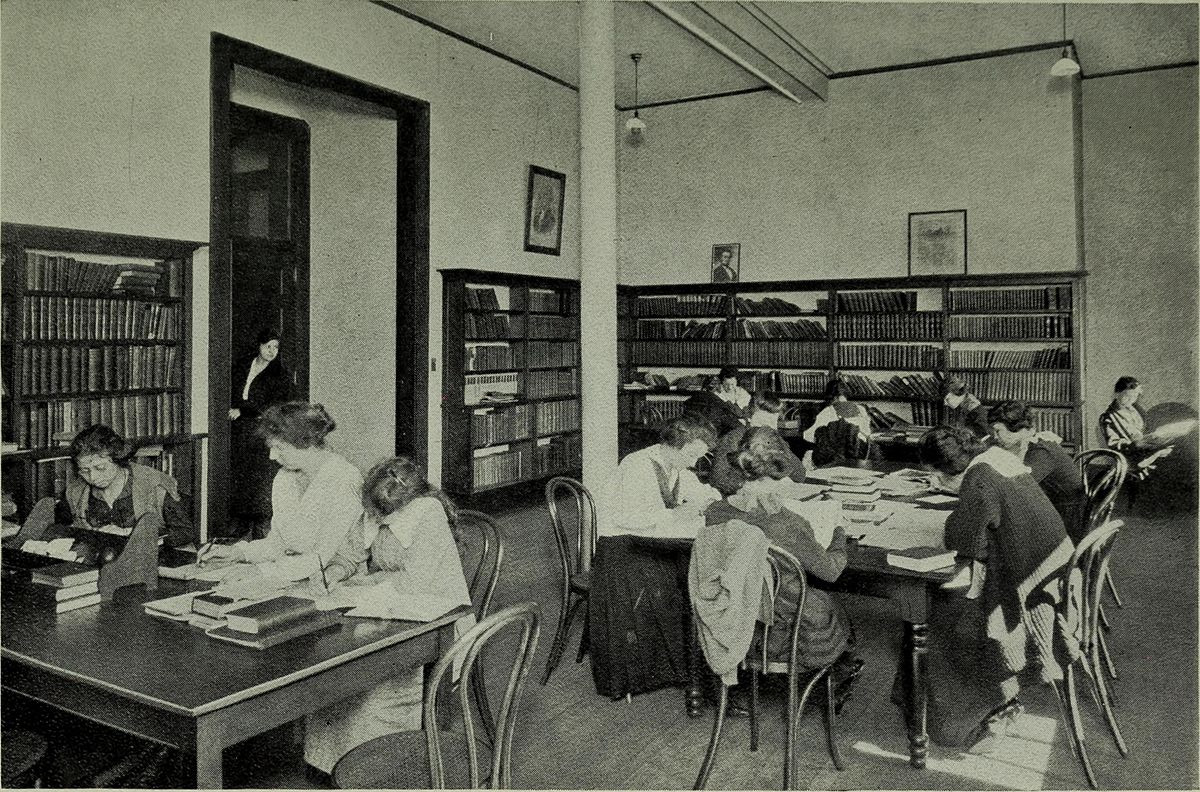
\includegraphics{images/ladies-hall.jpg}\\
\emph{Ladies Hall: Queens College, North Carolina.}

\hypertarget{whats-next-in-the-peeragogy-project}{%
\subsubsection{What's Next in the Peeragogy
Project}\label{whats-next-in-the-peeragogy-project}}

Making it easy and fruitful for others to get involved is one of the
best ways to redistribute the load. This often requires knowledge
transfer and skill development among those involved; see .

\hypertarget{references}{%
\subsubsection{References}\label{references}}

\begin{enumerate}
\def\labelenumi{\arabic{enumi}.}
\item
  Rishab A. Ghosh, Ruediger Glott, Bernhard Krieger, and Gregorio
  Robles. 2002. \emph{Free/Libre and Open Source Software: Survey and
  Study}. International Institute of Infonomics, University of
  Maastricht.
\item
  Mark Graham, Bernie Hogan, Ralph K Straumann, and Ahmed Medhat. 2014.
  Uneven geographies of user-generated information: Patterns of
  increasing informational poverty. \emph{Annals of the Association of
  American Geographers} 104, 4: 746--764.
\item
  Aaron Halfaker, R. Stuart Geiger, Jonathan Morgan, and John Riedl.
  2013. The Rise and Decline of an Open Collaboration System: How
  Wikipedia's reaction to sudden popularity is causing its decline.
  \emph{American Behavioral Scientist} 57, 5: 664--688.
  \url{http://doi.org/10.1177/0002764212469365}
\item
  Daniel Kreiss, Megan Finn, and Fred Turner. 2011. The limits of peer
  production: Some reminders from Max Weber for the network society.
  \emph{New Media \& Society} 13, 2: 243--259.
\item
  Mayo Fuster Morell. 2011. An introductory historical contextualization
  of online creation communities for the building of digital commons:
  The emergence of a free culture movement. \emph{Proceedings of the 6th
  Open Knowledge Conference}. Retrieved from
  \url{http://ceur-ws.org/Vol-739/paper_7.pdf}
\item
  Elinor Ostrom. 2010. Revising theory in light of experimental
  findings. \emph{Journal of Economic Behavior \& Organization} 73, 1:
  68--72.
\item
  François Rabelais. {[}1534{]} 1894. \emph{Gargantua and pantagruel}.
  Moray Press.
\item
  Eric S Raymond. 2001. \emph{The Cathedral \& the Bazaar: Musings on
  Linux and open source by an accidental revolutionary}. O'Reilly Media,
  Inc.
\item
  Joseph Reagle. 2012. ``Free as in sexist?'' Free culture and the
  gender gap. \emph{First Monday} 18, 1. Retrieved from
  \url{http://firstmonday.org/ojs/index.php/fm/article/view/4291}
\item
  Jaakko Seikkula and Tom Erik Arnkil. 2006. \emph{Dialogical meetings
  in social networks}. Karnac Books.
\item
  Tom Simonite. 2013. The Decline of Wikipedia. \emph{Technology Review}
  116, 6: 50--56.
\item
  Nassim Nicholas Taleb. 2012. \emph{Antifragile: Things that gain from
  disorder}. Random House Incorporated.
\item
  Linus Torvalds and Steven Vaughan-Nichols. 2011. Linus Torvalds's
  Lessons on Software Development Management. \emph{Input Output}.
  Retrieved from
  \url{http://web.archive.org/web/20131021211847/http://h30565.www3.hp.com/t5/Feature-Articles/Linus-Torvalds-s-Lessons-on-Software-Development-Management/ba-p/440}
\end{enumerate}

\begin{center}\rule{0.5\linewidth}{0.5pt}\end{center}

%
\section{A specific project} \label{sec:A specific project}
\hypertarget{a-specific-project}{%
\subsection{A specific project}\label{a-specific-project}}

\hypertarget{motivation}{%
\subsection{Motivation}\label{motivation}}

This pattern can help project participants get started, get focused, and
make concrete change. It is especially useful for someone who is
currently feeling stuck.

\hypertarget{context}{%
\subsection{Context}\label{context}}

We often find ourselves confronted with what seems to be a difficult,
complex, or even insurmountable problem. It won't go away, but a
workable solution doesn't present itself, either. If there is a
candidate solution, it's also clear there are not enough resources for
it to be feasible.

\hypertarget{forces}{%
\subsection{Forces}\label{forces}}

\begin{quote}
\Sdifficulty\ \textbf{Difficulty}: bringing about meaningful change is often hard work.\\
\Sinertia\ \textbf{Inertia}: when things are hard we may feel stuck, wring our hands, or preach to the choir.
\end{quote}

\hypertarget{problem}{%
\subsection{Problem}\label{problem}}

One is often blinded by one's prejudices and preferences. Some may put
considerable energy into pondering, discussing, exploring and feeling
stuck. Some may want more concrete progress, and notice the time passing
by. In a group setting, when the forward-movers ultimately try to act,
those who are more wrapped up in the experience of pondering and
exploring may rebel, if they feel that they are being left behind.
Inaction may seem like the only safe choice, but it has risks too. And,
once moving, things can easily get bogged down again.

\hypertarget{solution}{%
\subsection{Solution}\label{solution}}

One way to make progress when you're stuck is to ask a specific question
to someone who may be able to help you get unstuck. Formulating a
question helps your thinking become more concrete. Sometimes you'll see
that a solution was within your grasp all along. Often, one question
won't be enough, but you can repeat the process. In this way, you can
reduce a large, complex, or ephemeral concern into a collection of
smaller, specific, manageable tasks with clear next steps and success
criteria. Use a {{Scrapbook}} to make note of all the small things, and
weave them into your project {{Roadmap}}. This will show how the small
pieces relate to the bigger picture. If you have a fairly specific idea
about what you want to do, but you're finding it difficult to get it
done, don't just ask for advice: recruit material help (cf.~{{Carrying
capacity}}). One example of a specific project from the Peeragogy
project is our work on this paper, which had a specific target audience,
a set of associated deadlines, and allowed us to get help from pattern
experts.

\hypertarget{rationale}{%
\subsection{Rationale}\label{rationale}}

We've seen time and again that having a specific project is a recipe for
getting concrete, and that getting concrete is necessary for bringing
about change. Asking for help (which is what happens when you vocalize a
question) is one of the best ways to gain coherence. Making yourself
understood can go a long way toward resolving deeper difficulties.

\hypertarget{resolution}{%
\subsection{Resolution}\label{resolution}}

Where you run into \textbf{difficulty}, getting specific paves the way
for incremental forward progress and helps to overcome \textbf{inertia}.
The struggle between consensus and action is resolved in a tangible
project that combines action with dialog. Learning something new is a
strong sign that things are working. In the Peeragogy project, we have
completed many projects during our weekly hangouts, for example ``hive
editing'' an abstract for submission to a conference.

\hypertarget{example-1}{%
\subsection{Example 1}\label{example-1}}

At first glance, the Wikimedia Foundation's mission may seem like a good
idea, but hard to do anything about.\footnote{\url{https://wikimediafoundation.org/wiki/Mission_statement}}
practice, many Wikipedians contribute to the mission by working on {{A
specific project}}.

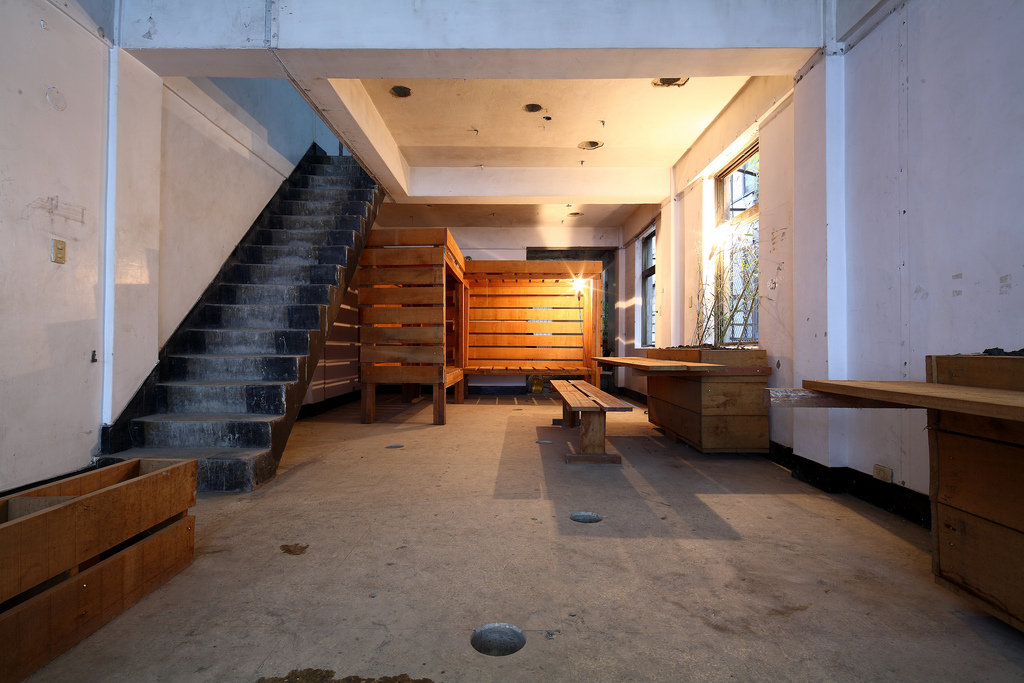
\includegraphics{images/Ruin_Academy_Dorm.jpg} \emph{Dormitory, Ruin
Academy, Taipei, Taiwan.}

Within Wikipedia, these are known as
``WikiProjects.''\footnote{\url{https://en.wikipedia.org/wiki/Wikipedia:WikiProject_Council/Directory}},\footnote{\^{}fn3}
on how to start new WikiProjects.\footnote{\url{https://en.wikipedia.org/wiki/Wikipedia:WikiProject_Council/Guide/WikiProject}}
Wikimedia Foundation also runs other public projects, including the
Wikipedia Education Program and the GLAM Wiki (for Galleries, Libraries,
Archives, and Museums).\footnote{\url{https://outreach.wikimedia.org/wiki/Education/Wikipedia_Education_Collaborative/Tasks}},\footnote{\url{https://outreach.wikimedia.org/wiki/GLAM}}
\emph{list of case studies that describes specific projects undertaken
by cultural organizations and Wikimedia}.\footnote{\url{https://outreach.wikimedia.org/wiki/GLAM/Case_studies}}

\hypertarget{example-2}{%
\subsection{Example 2}\label{example-2}}

Collegial and convivial peer support via remote collaboration or
short-term meet-ups may fill some of the requirements of ``student
life''. Peeragogy can also happen in neighborhoods, and among persons
sharing long-term co-habitation. While a traditional Dormitory may not
be necessary, a shared rented or cooperatively-owned living/working
environment could be an asset for peeragogues working together on {{A
specific project}}.

\hypertarget{whats-next-in-the-peeragogy-project}{%
\subsection{What's Next in the Peeragogy
Project}\label{whats-next-in-the-peeragogy-project}}

Let's use our pattern catalog to build specific, tangible ``what's
next'' steps, add them to our {{Roadmap}}, and carry them out with
concrete actions. Let's be sure we know who's responsible for what, and
employ a ``buddy system'' to help get things done.

\begin{center}\rule{0.5\linewidth}{0.5pt}\end{center}

%
\section{Wrapper} \label{sec:Wrapper}
\section{Wrapper}\label{wrapper}

\subsubsection{Context}\label{context}

An active project with more than a few participants, and possibly with
{\textbf{Newcomers}} arriving frequently.

\subsubsection{Problem}\label{problem}

In a very active project, it can be effectively impossible to stay up to
date with all of the details. Not everyone will be able to attend every
meeting (see
{\textbf{\href{http://peeragogy.org/patterns/heartbeat/}{Heartbeat}}})
or read every email, and project participants can easily get lost and
drift away. The experience can be even worse for {\textbf{Newcomers}}:
joining a project already going can feel like trying to get aboard a
rapidly moving vehicle. If you've taken time off, you may feel like
things have moved on so far that they cannot catch up.

\subsubsection{Solution}\label{solution}

A project contributor can summarize what has happened recently in the
project, making progress comprehensible to participants who have not
been following all of the details.\footnote{In the Peeragogy project,
  this idea was initially suggested by Charlie Danoff, adapting an idea
  from his Indiana University class on EFL teaching led by Faridah
  Pawan. The idea was that someone take on the ``wrapper role'' -- do a
  weekly pre/post wrap, so that new (and existing) users could get a
  feel for the status of the project at any given point in time.} If
they are kept up to date, a project's
\href{http://socialmediaclassroom.com/host/peeragogy/}{landing page} and
{\textbf{Roadmap}} also serve as a sort of ``wrapper'', telling people
what resources they can expect to find in the project and how they can
participate.

\subsubsection{Rationale}\label{rationale}

The wrapper must check the public summaries of the project from time to
time to make sure that they accurately represent the facts on the
ground.\footnote{In the first year of the Peeragogy project, the
  ``Weekly Roundup'' by Christopher Tillman Neal served to engage and
  re-engage members. Peeragogues began to eagerly watched for the weekly
  reports to see if our teams or our names had been mentioned. When
  there was a holiday or break, Chris would announce the hiatus, to keep
  the flow going. In the second year of the project, we did not
  routinely publish summaries of progress, and instead, we assumed that
  interested parties will stay tuned on Google+. More recently, Charlie
  has begun publishing irregular wrap-up
  \href{http://peeragogy.org/peeragogy-wrapper-post-9-feb-5-apr-2015/}{blog
  posts} and e-mails again, which helps keep people who don't read
  Google+ up to date.}

\subsubsection{Resolution}\label{resolution}

According to the theory proposed by Yochai Benkler, for free/open
``commons-based'' projects to work, it is vital to have both (1) the
ability to contribute small pieces; (2) something that stitches those
pieces together @coases-penguin. The wrapper helps perform this
integrative stitching function, which is often much more challenging
than the job of breaking things down into pieces or just doing one of
the small pieces.

\subsubsection{What's Next}\label{whats-next}

We need better practices for automating the wrapping-up process. One of
the latest ideas is to develop a simple visual ``dashboard'' for the
project that would be a web page people could access and immediately get
an idea of what work is ongoing in the project with links for going more
in depth and/or contributing.

%
\section{Heartbeat} \label{sec:Heartbeat}
\hypertarget{heartbeat}{%
\subsection{Heartbeat}\label{heartbeat}}

\hypertarget{motivation}{%
\subsubsection{Motivation}\label{motivation}}

This pattern can help project participants stay in touch, and stay
motivated.

\hypertarget{context}{%
\subsubsection{Context}\label{context}}

A number of people have a shared interest, and have connected with each
other about it. However, they are not going to spend 24 hours a day, 7
days a week working together, either because they are busy with other
things, or because working separately on some tasks is vastly more
efficient.

\hypertarget{forces}{%
\subsubsection{Forces}\label{forces}}

\begin{quote}

\includegraphics{images/differentiation.png} \textbf{Differentiation}:
the time we spend together isn't all equally meaningful.\\

\includegraphics{images/entropy.png} \textbf{Entropy}: something needs
to hold the project together, or it will fall apart.
\end{quote}

\hypertarget{problem}{%
\subsubsection{Problem}\label{problem}}

How will the effort be sustained and coordinated sufficiently? How do we
know this an active collaboration, and not just a bunch of people
milling about? Is there a \emph{there, there?}

\hypertarget{solution}{%
\subsubsection{Solution}\label{solution}}

People seem to naturally gravitate to something with a pulse. \emph{Once
a day} (stand-ups), \emph{once a week} (meetings), or \emph{once a year}
(conferences, festivals) are common variants. When the project is
populated by more than just a few people, it's likely that there will be
several {{Heartbeats}}, building a sophisticated polyrhythm. A
well-running project will feel ``like an improvisational jazz ensemble''
{{[}1{]}}. Much as the band director may gesture to specific players to
invite them to solo or sync up, a project facilitator may craft
individual emails to ask someone to lead an activity or invite them to
re-engage. Two common rhythm components are weekly synchronous meetings
with an open agenda, combined with \emph{ad hoc} meetings for focused
work on {{A specific project}}. The precise details will depend on the
degree of integration required by the group.

\hypertarget{rationale}{%
\subsubsection{Rationale}\label{rationale}}

The project's heartbeat is what sustains it. Just as \emph{people matter
more than code} {{[}2{]}}, so does the life of the working group matter
more than mechanics of the work structure. Indeed, there is an quick way
to do a reality check and find the project's strongest pulse: the
activities that sustain a healthy project should sustain us, too
(cf.~{{Carrying capacity}}).

\hypertarget{resolution}{%
\subsubsection{Resolution}\label{resolution}}

Noticing when a new {{Heartbeat}} is beginning to emerge is a way to be
aware of the shifting priorities in the group, and contributes to
further \textbf{differentiation}. This may ultimately be a good source
of new patterns. On the other hand, if a specific activity is no longer
sustaining the project, stop doing it, much as you would move an
out-of-date pattern to the {{Scrapbook}} in order to make room for other
concerns. The power of the {{Heartbeat}} is that the project can be as
focused and intensive as it needs to be, working against
\textbf{entropy} in the ways that start to be required as time goes by.

\hypertarget{example-1}{%
\subsubsection{Example 1}\label{example-1}}

The yearly in-person gathering, Wikimania, is the most visible example
of a {{Heartbeat}} for the Wikimedia movement.\footnote{\url{https://meta.wikimedia.org/wiki/Wikimania}}
may run additional in-person get-togethers.\footnote{\url{http://wikiconferenceusa.org/}}
Also of note is the twice-yearly call for proposals for individual
engagement grants.\footnote{\url{https://meta.wikimedia.org/wiki/Grants:IEG}}
other shorter cycles. Each day a highly-vetted Featured Article appears
on the front page of Wikipedia, and is circulated to a special-purpose
mailing list.\footnote{\url{https://en.wikipedia.org/wiki/Wikipedia:Today\%27s_featured_article}},\footnote{\url{https://en.wikipedia.org/wiki/Wikipedia:Featured_article_candidates}},\footnote{\url{https://lists.wikimedia.org/mailman/listinfo/daily-article-l}}
articles for deletion lasts at least seven days.\footnote{\url{https://en.wikipedia.org/wiki/Wikipedia:Articles_for_deletion}}

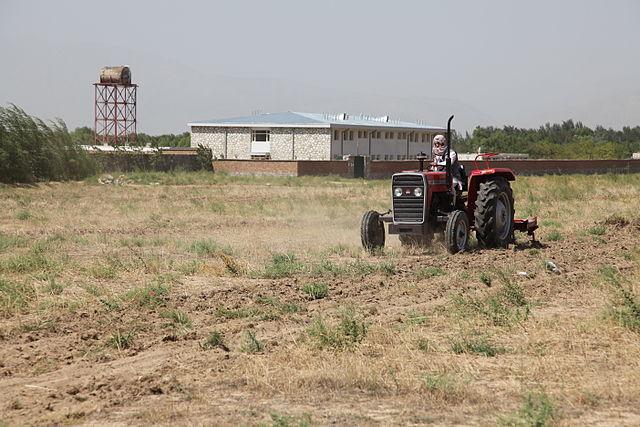
\includegraphics{images/kapisa.jpg}\\
\emph{University Farm: al-Biruni University, Kapisa province,
Afghanistan.}

\hypertarget{example-2}{%
\subsubsection{Example 2}\label{example-2}}

Although it may sound quaint, some variant of the University Farm could
help to physically sustain peeragogues, while putting the project's
{{Heartbeat}} in tune with that of the seasons. In the current
distributed mode, we tend our window boxes and allotment gardens. New
developments should unfold in a \emph{logical order growing out of the
needs of the community} {{[}3{]}}.

\hypertarget{whats-next-in-the-peeragogy-project}{%
\subsubsection{What's Next in the Peeragogy
Project}\label{whats-next-in-the-peeragogy-project}}

\begin{quote}
Actual meeting times to be added
\end{quote}

Identifying and fostering new {{Heartbeats}} and new working groups can
help make the community more robust. This is the time dimension of
spin-off projects described in {{Reduce, reuse, recycle}}.

\hypertarget{references}{%
\subsubsection{References}\label{references}}

\begin{enumerate}
\def\labelenumi{\arabic{enumi}.}
\item
  David M. Dikel, David Kane, and James R. Wilson. 2001. \emph{Software
  architecture: Organizational principles and patterns}. Pearson
  Education.
\item
  Linus Torvalds and Steven Vaughan-Nichols. 2011. Linus Torvalds's
  Lessons on Software Development Management. \emph{Input Output}.
  Retrieved from
  \url{http://web.archive.org/web/20131021211847/http://h30565.www3.hp.com/t5/Feature-Articles/Linus-Torvalds-s-Lessons-on-Software-Development-Management/ba-p/440}
\item
  Booker T Washington. 1901. \emph{Up from slavery}. Doubleday \&
  Company, Inc.
\end{enumerate}

\begin{center}\rule{0.5\linewidth}{0.5pt}\end{center}

%
\section{Newcomer} \label{sec:Newcomer}
\begin{refsection}

% DK: I am not sure that this is a Pattern. It is a role for sure, but is it a solution to a problem? Maybe the name of the pattern is wrong. Something like Welcome Wagon? Something that evokes the response to the Newcomer.

\paragraph{Motivation} This pattern can help project participants be aware of the issues faced by newcomers, and cultivate a ``beginner's mind'' themselves.

\paragraph{Context}
% DK: This is an interesting point. I am not sure it is Context. Maybe Rationale?
When there's learning happening, it's because there is someone who is new to a topic, or to something about the topic.

\bgroup
\def\arraystretch{1.2}%
\paragraph{Forces}~\hspace{-.04\textwidth}
\begin{tabular}[t]{p{.7\textwidth}@{\hspace{.05\textwidth}}c}
\textbf{Individuation}: each person learning optimally is what's best for the community. & {\icon \symbol{"0021E5}} \\
\textbf{Mutuality}: our individuality does not isolate us from one another, but draws us together. & 
{\icon \symbol{"002180}}%{\icon \symbol{"002117}}
\\
\end{tabular}
\egroup

\paragraph{Problem} Newcomers can feel overwhelmed by the amount of things to learn.  They
often don't know where to start.  They may have a bunch of ideas that the
oldtimers have never considered -- or they may think they have new
ideas, which are actually a different take on an old idea; see
\patternname{Reduce, reuse, recycle}. People who are new to the project can tell you what makes their participation difficult.  Since you're learning as you go as well, you can ask yourself the same question: what aspects of this encounter are difficult for me?  

% DK: This seems a little spare
\paragraph{Solution}

Instead of thinking of newcomers as ``them'', and trying to provide
solutions, we focus on newcomers as ``us'' -- which makes the search
for solutions that much more urgent.  We permit ourselves to ask naive
questions.  We entertain vague ideas.  We add concreteness by trying
\patternname{A specific project}.  We may then genuinely turn to
others for help.
% OSS: What about action research?
% similar... not handholding but interactive
We aim to foster a culture in which the focus for everyone is on
addressing our own learning challenges rather than on ``providing''
solutions for others \cite{boud2005peer}.
%
When you begin a new project, try to systematically take notes and
gather data to analyze and reflect upon later; leave artifacts for
other future newcomers to use and build upon in their own research.
In practice this may be a lot to ask for someone just joining a group,
but over time we may have many ways to structure our collective
engagement so that it leads to research cycles based on the ``action
research'' steps \emph{reflect}, \emph{plan}, \emph{act}, and
\emph{observe}.
% \footnote{\url{https://valenciacollege.edu/faculty/development/tla/actionResearch/ARP_softchalk/mobile_pages/index.html}}
Note that there is a parallel with the four facets \emph{assess},
\emph{convene}, \emph{organize}, \emph{cooperate} from Figure
\ref{fig:connections}.  The history of the action research approach,
with particular emphasis on educational applications, is surveyed in
\cite[Chapter 3]{mcniff2013action}.  One method for doing the
reflection\slash assessment step is presented in the
\patternname{Scrapbook} pattern.
%% Another related model is Wallas's \cite{wallas1926art} four-part model
%% of creative thought, consisting of repeated or overlapping cycles of
%% \emph{preparation}, \emph{incubation}, \emph{illumination}, and
%% \emph{verification}.
%% The ``cyclic'' aspect of such models is less
%% important than the fact that they they point out key ingredients for
%% constructive engagement \cite{engestrom199923}.
Be flexible: networked attention (even more so than rigid cycles
\cite{engestrom199923}) leads to new ways of knowing and expanded
access to knowledge-production \cite{gilbert2012being,wagner2008new}.


% DK: I can empathize :+) I wonder if there is a pattern that is missing. Vision? A clear articulation about what the effort is for
%
\paragraph{Rationale} 
%
A newcomer's confusion about how best to get involved or what the
point of all this actually is may be due to a lack of structure in the
project \patternname{Roadmap}.  Sharing vulnerability and confusion
gives us a chance to learn.
%
%% In the words of Antoine de Saint-Exup\'ery:
%% ``If you want to build a boat, do not instruct the men to saw wood,
%% stitch the sails, prepare the tools and organize the work,
%% but make them long for setting sail and travel to distant lands.''

% DK: The resolution should describe the circumstance after applying the solution. This seems to be describe the circumstance without the solution.
\paragraph{Resolution}
An awareness of the difficulties that newcomers face can help us be
more compassionate to ourselves and others.  We strengthen the
community by supporting all participants' \textbf{individuation}.  We
have a better chance of making the project useful for others if we're
clear about how it is useful to \emph{us}.  By welcoming newcomers, we
enhance the sense of \textbf{mutuality} with people who have never
encountered the project before, and learn together with them.  The
facts start to become useful when we understand how people perceive
them \cite{freire1982creating}.

%% the concrete reality consists not only of concrete facts and
%% (physical) things, but also includes the ways in which the people
%% involved with these facts perceive them. Thus in the last analysis,
%% for me, the concrete reality is the connection between subjectivity
%% and objectivity, never objectivity isolated from subjectivity.

\paragraph{Example 1} Wikipedia \patternnameplural{Newcomer} can make use of resources that
include a ``Teahouse'' where questions are welcomed, a platform
extension that changes the user interface for new editors, and lots of
documentation.\footnote{\url{https://en.wikipedia.org/wiki/Wikipedia:Teahouse}}%
\textsuperscript{,}\footnote{\url{https://en.wikipedia.org/wiki/Wikipedia:GettingStarted}}%
\textsuperscript{,}\footnote{\url{https://en.wikipedia.org/wiki/Help:Editing}}
The efforts of exceptional newcomers may be given special
recognition.\footnote{\url{https://en.wikipedia.org/wiki/Template:The_New_Editor\%27s_Barnstar}}
Newcomer ``survival'' is of interest to the Wikimedia
Foundation.\footnote{\url{https://meta.wikimedia.org/wiki/Research:Newcomer_survival_models}}
However, ``Nearly all editors begin with a burst of activity, then
quickly tail off'' \cite{panciera2009wikipedians}.  The degree to
which those editors who are retained emphasize continuous upskilling
is somewhat less clear.  As regards learning their way around the
community, quantitative support exists \cite{panciera2009wikipedians}
for the claim that ``novice users learn the rules and conventions for
contributing both through observation and direct coaching from more
knowledgeable others'' \cite{bryant2005becoming}.

\begin{wrapfigure}{r}{.47\textwidth}
\vspace{-.2cm}
\begin{center}
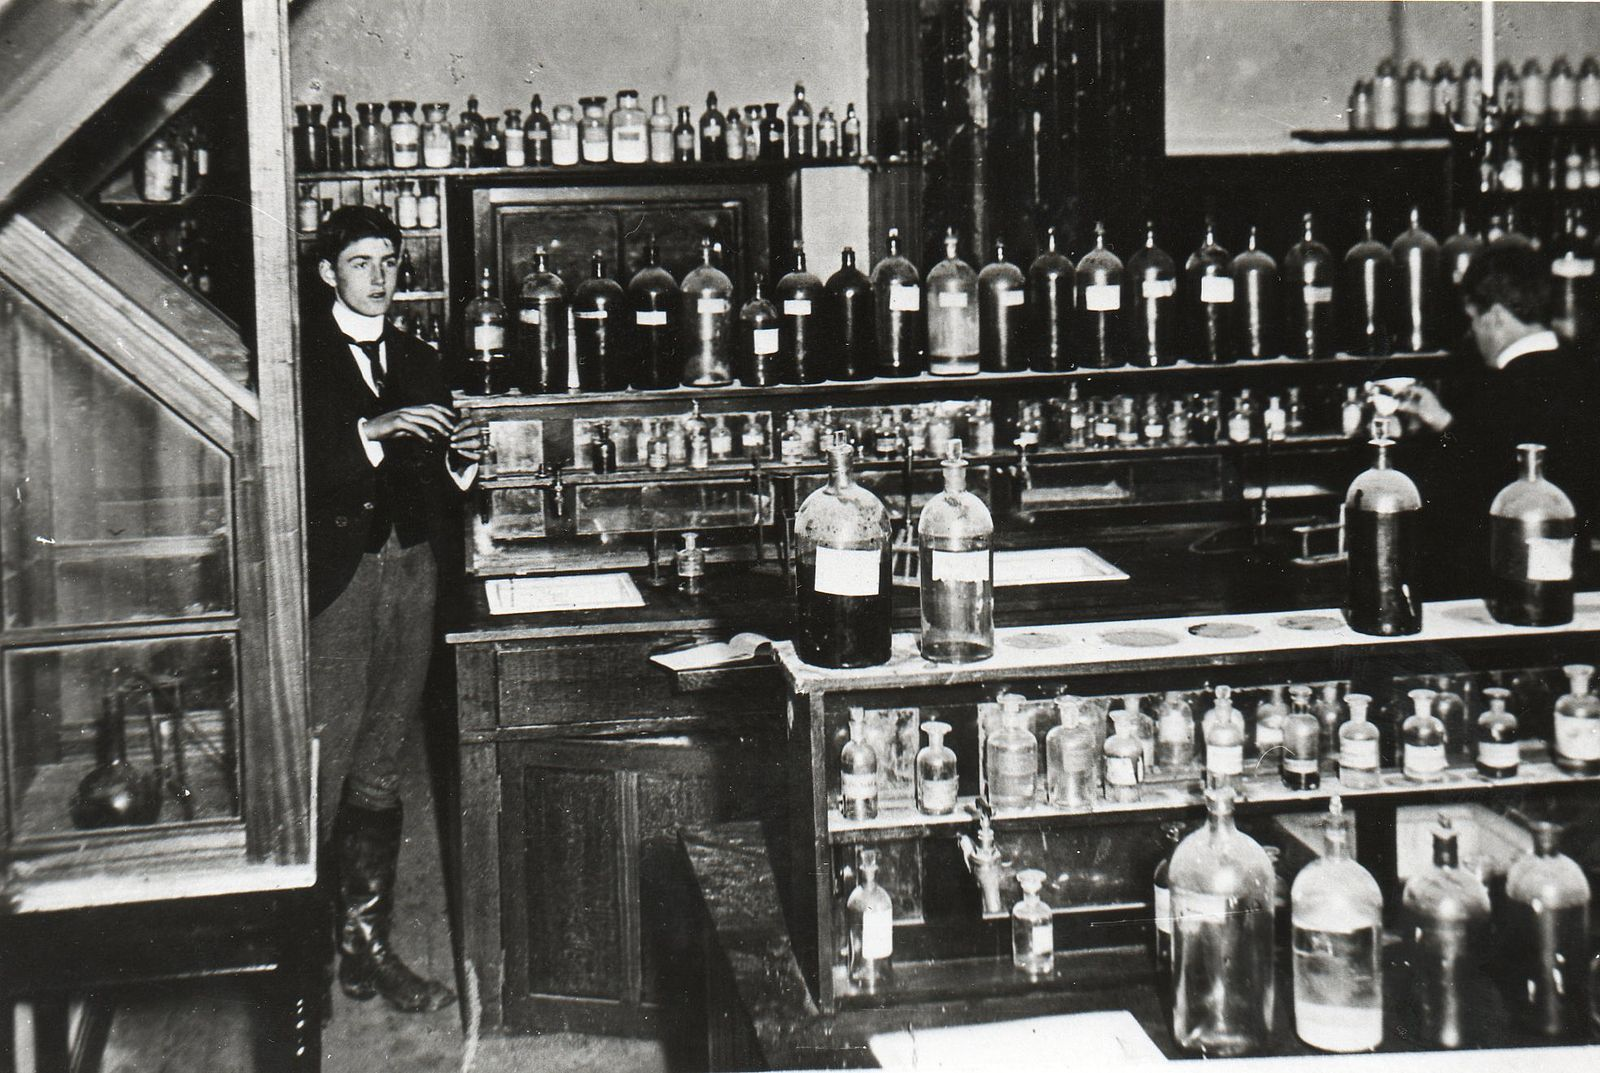
\includegraphics[width=.45\textwidth]{../pictures/The_Science_Laboratory.jpg}
\end{center}
\vspace{-.5cm}
\caption{Science Laboratory, Aspatria Agricultural College, Cumberland, UK. 
% Public domain.
\label{science-laboratory}}
\vspace{-.1cm}
\end{wrapfigure}

\paragraph{Example 2} It will often be pragmatic to connect
\patternnameplural{Newcomer} with employment directly, so that
the future university may see a closer coupling of science and
industry than would be found in the old Science Hall.  Inspiration can
be drawn the London-based freelancing cooperative Founders\&Coders,
which is able to offer intensive training in web development at no
cost to successful applicants.


\begin{framed}
\noindent 
\emph{What's Next in the Peeragogy Project}
\definecollection{NewcomerWN}
\begin{collectinmacro}{\NewcomerWN}{}{}
More detailed guides can show \patternnameplural{Newcomer}  how they can contribute and what to expect when they do. We should have different guides for different ``user stories''. We can start by listing some of the things we're currently learning about.
\end{collectinmacro}
\NewcomerWN
\end{framed}

\printbibliography[heading=subbibliography]
\end{refsection}

%
\section{Scrapbook} \label{sec:Scrapbook}
\hypertarget{scrapbook}{%
\subsection{Scrapbook}\label{scrapbook}}

\hypertarget{motivation}{%
\subsection{Motivation}\label{motivation}}

This pattern describes a way to make the project meaningful.

\hypertarget{context}{%
\subsection{Context}\label{context}}

We have been working together for a while now. We have maintained and
revised our pattern catalog, and we are achieving some of the ``What's
Next'' steps associated with some of the patterns.

\hypertarget{forces}{%
\subsection{Forces}\label{forces}}

\begin{quote}
\Sattention\ \textbf{Attention}: due to limited energy, we need to ask: where should we set the focus?
\Sinterest\ \textbf{Interest}: new experiences catch our attention.
\Smeaning\ \textbf{Meaning}: shared history makes things meaningful.
\end{quote}

\hypertarget{problem}{%
\subsection{Problem}\label{problem}}

Not all of the ideas we've come up with have proved workable. Not all of
the patterns we've noticed remain equally relevant. In particular, some
patterns no longer lead to concrete next steps.

\hypertarget{solution}{%
\subsection{Solution}\label{solution}}

In order to maintain focus, is important to ``tune'' and ``prune'' the
things we give our attention to. We can connect this understanding to
any actions undertaken in the project by asking questions like these:

\begin{quote}
(1) Review what was supposed to happen. (2) Establish what is
happening/happened. (3) Determine what's right and wrong with what we
are doing/have done. (4) What did we learn or change? (5) What else
should we change going forward? {{[}9{]}}, after {{[}10{]}}.
\end{quote}

Other review processes have been formalized, including the design review
in architecture and the postmortem in theater and other teamwork
settings {{[}7,8{]}}. The review process may benefit from having an
experienced facilitator on board {{[}6{]}}. As current priorities become
clearer, we decide where to focus. Anything that isn't receiving active
attention should be moved to a {{Scrapbook}}. This may encompass:

\begin{itemize}
\tightlist
\item
  \emph{Retired patterns} that are tabled or completed (no more next
  steps);
\item
  \emph{Proto-patterns} made of problems, issues, and concerns;
\item
  \emph{A back-catalog} of publications, reports, or other artifacts.
\end{itemize}

In the Peeragogy project, alongside our patterns we initially maintained
a collection of antipatterns (like `{{Magical thinking}}') but the next
steps coming from these seemed particularly convoluted and abstract. So,
we archived them.\footnote{\url{http://paragogy.net/Scrapbook}} problems
-- without known solutions -- right up front in the Introduction to the
\emph{Peeragogy Handbook} {{[}9{]}}. Other proto-patterns include
`{{Onboarding}}' and `{{Don't quit your day job}}', which arose in our
review of this paper (see ``Emergent Roadmap'', below). Our back-catalog
includes academic papers {{[}14{]}} and a thesis {{[}5{]}}. Everyone can
maintain their own personal {{Scrapbook}} as along with a communal one.
Furthermore, you don't need to limit yourself to \emph{your own}
creativity: include interesting ideas from other sources (see {{Reduce,
reuse, recycle}}). In some cases a designated {{Wrapper}} may have to do
further work to elicit and organize contributions.

\hypertarget{rationale}{%
\subsection{Rationale}\label{rationale}}

We want to keep attention focused on the most relevant issues. If a
pattern, task, or concern does not lead to concrete ``next steps'' at
the moment, sufficient time for reflection may offer a better
understanding, and it may prove useful and actionable in a different
context.

\hypertarget{resolution}{%
\subsection{Resolution}\label{resolution}}

Judicious use of the {{Scrapbook}} can help focus project participants'
\textbf{attention} on current concerns, without losing grasp of items of
\textbf{interest}. The currently active pattern catalog is leaner and
more action-oriented as a result. If the {{Roadmap}} shows where we're
going, it is the {{Scrapbook}} that shows most clearly where we've been,
and collects the observations that are most \textbf{meaningful} to us.

\hypertarget{example-1}{%
\subsection{Example 1}\label{example-1}}

The history of the Wikimedia Foundation, and of Wikipedia, are
maintained as wiki pages.\footnote{\url{https://wikimediafoundation.org/wiki/History_of_the_Wikimedia_Foundation}},\footnote{\url{https://en.wikipedia.org/wiki/Wikipedia}}
Wikipedia details outstanding issues, in the form of
critiques.\footnote{\url{https://en.wikipedia.org/wiki/Criticism_of_Wikipedia}}
available to help facilitate the process of vetting proposed
fine-grained changes to articles.\footnote{\url{https://en.wikipedia.org/wiki/Special:RecentChanges}},\footnote{\url{https://en.wikipedia.org/wiki/Wikipedia:Recent_changes_patrol\#Tools}}
typically discussed at the Village Pump, and there are mechanisms in
place for settling disputes.{[}\^{}7\^{}{]},\footnote{\url{https://en.wikipedia.org/wiki/Wikipedia:Requests_for_comment}}

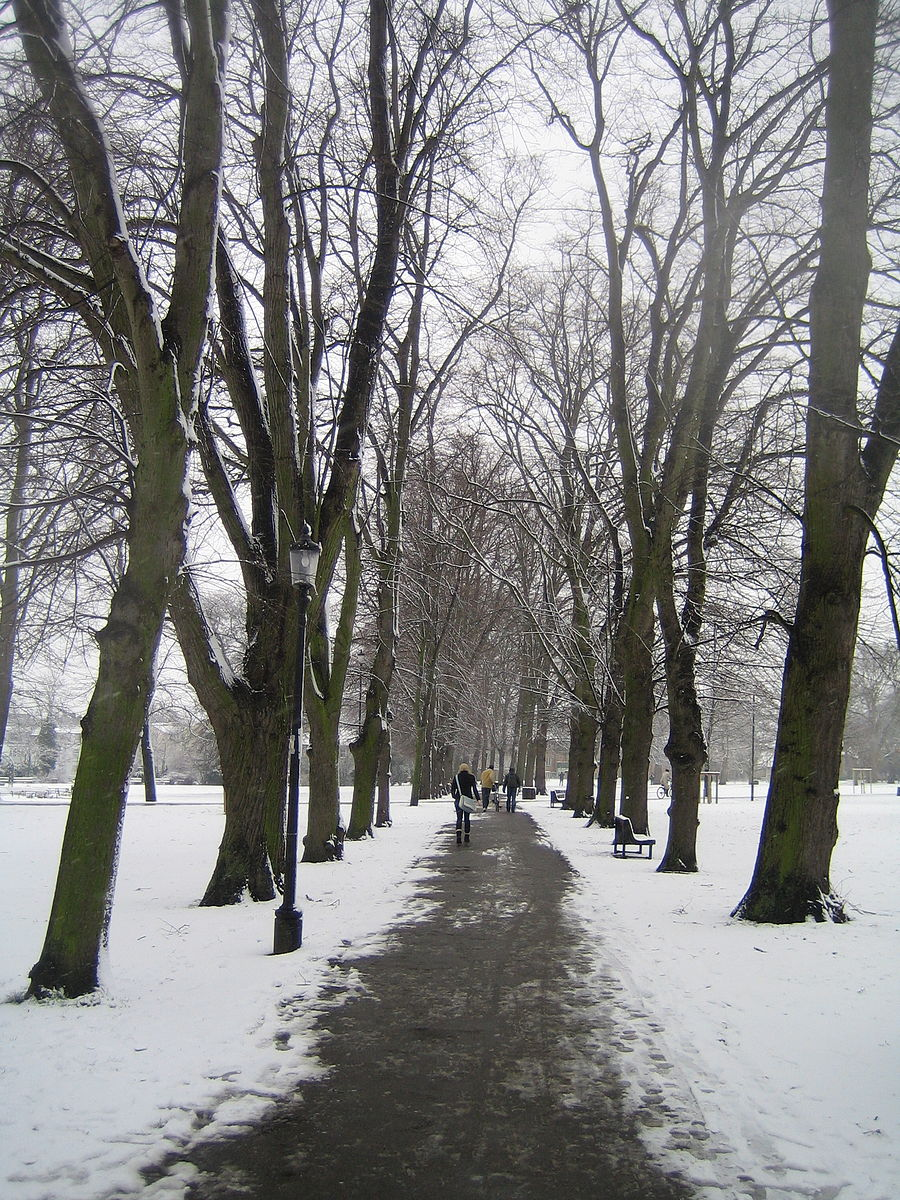
\includegraphics{images/ChristsPieces.jpg}\\
\emph{Park: Christ's Pieces, Cambridge, UK}

\hypertarget{example-2}{%
\subsection{Example 2}\label{example-2}}

Just as a university campus grows and changes over time, future
peeragogues will be drawn to new problems and patterns. They will trace
new paths and build new emergent structures (Figure
{[}christs-pieces{]}).

\hypertarget{whats-next-in-the-peeragogy-project}{%
\subsection{What's Next in the Peeragogy
Project}\label{whats-next-in-the-peeragogy-project}}

After pruning back our pattern catalog, we want it to grow again: new
patterns are needed. One strategy would be to turn the whole
\emph{Peeragogy Handbook} into design patterns.

\hypertarget{references}{%
\subsection{References}\label{references}}

\begin{enumerate}
\def\labelenumi{\arabic{enumi}.}
\item
  J Corneli, A Keune, A Lyons, and CJ Danoff. 2013. Peeragogy in Action.
  In \emph{The Open Book}, Kaitlyn Braybrooke, Jussi Nissilä and Timo
  Vuorikivi (eds.). The Finnish Institute, London, 80--87.
\item
  J. Corneli. 2012. Paragogical praxis. \emph{E-Learning and Digital
  Media} 9, 3: 267--272. Retrieved from
  \url{http://paragogy.net/ParagogicalPraxisPaper}
\item
  J. Corneli and C.J. Danoff. 2011. Paragogy. \emph{Proceedings of the
  6th Open Knowledge Conference}. Retrieved from
  \url{http://ceur-ws.org/Vol-739/paper+5.pdf}
\item
  Joseph Corneli, Dorota Marciniak, Charles Jeffrey Danoff, et al.~2014.
  Building the Peeragogy Accelerator. \emph{Proceedings of OER14:
  Building communities of open practice}. Retrieved from
  \url{http://metameso.org/~joe/docs/Building_the_Peeragogy_Accelerator.pdf}
\item
  Joseph Corneli. 2014. Peer produced peer learning: A mathematics case
  study. Retrieved from \url{http://oro.open.ac.uk/40775/}
\item
  Richard P Gabriel. 2002. \emph{Writer's Workshops and the Work of
  Making Things: Patterns, Poetry.} Addison-Wesley Longman Publishing
  Co., Inc.
\item
  Norman Kerth. 2001. \emph{Project retrospectives: A handbook for team
  reviews}. Dorset House.
\item
  John Mathers, Sue Illman, Angela Brady, and Peter Geraghty. 2013.
  Design Review: Principles and Practice. Retrieved from
  \url{http://www.rtpi.org.uk/media/11214/dc_cabe_design_review_13_w__1_.pdf}
\item
  H. Rheingold and others. 2015. \emph{The Peeragogy Handbook}.
  PubDomEd/Pierce Press, Chicago, IL./Somerville, MA. Retrieved from
  \url{http://peeragogy.org}
\item
  US Army. 1993. A Leader's Guide to After-Action Reviews (TC 25-20).
  Retrieved from
  \url{http://www.au.af.mil/au/awc/awcgate/army/tc_25-20/tc25-20.pdf}
\end{enumerate}

\begin{center}\rule{0.5\linewidth}{0.5pt}\end{center}


%%% \hypertarget{patterns-of-peeragogy}{%
\subsection{Patterns of Peeragogy}\label{patterns-of-peeragogy}}

This chapter outlines an approach to the organization of learning that
draws on the principles of free/libre/open source software (FLOSS), free
culture, and peer production. Mako Hill suggests that one recipe for
success in peer production is to take a familiar idea -- for example, an
encyclopedia -- and make it easy for people to participate in building
it {{[}11{]}}. We will take hold of ``learning in institutions'' as a
map, although it does not fully conform to our chosen tacitly-familiar
territory of \emph{peeragogy}. To be clear, peeragogy is for \emph{any
group of people who want to learn anything}.\footnote{\url{https://www.youtube.com/watch?v=TDRGJzoNbAc}}

\includegraphics{images/wisconsin-map.jpg}\\
\emph{A prototypical university. Caption reads: Wisconsin State
University, Madison, Wis. 1879. Inset captions describe the pictured
buildings: Ladies Hall, South Dormitory, University Hall, Assembly Halls
\& Library, North Dormitory, Science Hall, President's Residence,
University Farm, and Washburn Observatory. Public domain.}

Despite thinking about learning and adaptation that may take place far
outside of formal institutions, the historical conception of a
university helps give shape to our inqury. The model university is not
separate from the life of the state or its citizenry, but aims to
``assume leadership in the application of knowledge for the direct
improvement of the life of the people in every sphere'' {{[}8{]}}.
Research that \emph{adds to the store of knowledge} is another
fundamental obligation of the university {{[}8{]}}. The university
provides a familiar model for collaborative knowledge work but it is not
the only model available. Considering the role of collaboration in
building Wikipedia, StackExchange, and free/libre/open source software
development, we may be led to ask: What might an accredited
free/libre/open university look like? How would it compare or contrast
with the typical or stereotypical image of a university from the figure
above? Would it have similar structural features, like a Library,
Dormitory, Science Hall and so on? Would participants take on familiar
roles {{[}5{]}}? How would it compare with historical efforts like the
Tuskegee Institute that involved students directly in the production of
physical infrastructure {{[}7,19{]}}? We use the word \emph{peeragogy}
to talk about collaboration in relatively non-hierarchical settings.
Examples are found in education, but also in business, government,
volunteer, and NGO settings. Peeragogy involves both problem solving and
problem definition. Indeed, in many cases it is preferable to focus on
solutions, since people know the ``problems'' all too well {{[}2{]}}.
Participants in a peeragogical endeavor collaboratively build emergent
structures that are responsive to their changing context, and that in
turn, change that context. In the Peeragogy project, we are developing
the the theory and practice of peeragogy.

\emph{Design patterns} offer a methodological framework that we have
used to clarify our focus and organize our work. A design pattern
expresses a commonly-occurring problem, a solution to that problem, and
rationale for choosing this solution {{[}13{]}}. This skeleton is
typically fleshed out with a \emph{pattern template} that includes
additional supporting material; individual patterns are connected with
each other in a \emph{pattern language}. What we present here is rather
different from previous pattern languages that touch on similar topics
-- like \emph{Liberating Voices} {{[}17{]}}, \emph{Pedagogical Patterns}
{{[}3{]}}, and \emph{Learning Patterns} {{[}12{]}}. At the level of the
pattern template, our innovation is simply to add a ``What's next''
annotation, which anticipates the way the pattern will continue to
``resolve''.

This addition mirrors the central considerations of our approach, which
is all about human interaction, and the challenges, fluidity and
unpredictability that come with it. Something that works for one person
may not work for another or may not even work for the same person in a
slightly different situation. We need to be ready to clarify and adjust
what we do as we go. Even so, it is hard to argue with a
sensible-sounding formula like ``If W applies, do X to get Y.'' In our
view, other pattern languages often achieve this sort of common sense
rationality, and then stop. Failure in the prescriptive model only
begins when people try to define things more carefully and make
context-specific changes -- when they actually try to put ideas into
practice. The problem lies in the inevitable distance between \emph{do
as I say}, \emph{do as I do}, and \emph{do with me} {{[}9{]}}. If people
are involved, things get messy. They may think that they are on the same
page, only to find out that their understandings are wildly different.
For example, everyone may agree that the group needs to go ``that way.''
But how far? How fast? It is rare for a project to be able to set or
even define all of the parameters accurately and concisely at the
beginning. And yet design becomes a ``living language'' {{[}1{]}} just
insofar as it is linked to action. Many things have changed since
Alexander suggested that ``you will get the most `power' over the
language, and make it your own most effectively, if you write the
changes in, at the appropriate places in the book'' {{[}1{]}}. We see
more clearly what it means to inscribe the changing form of design not
just in the margins of a book, or even a shared wiki, but in the
lifeworld itself. Other recent authors on patterns share similar views
{{[}15,16,18{]}}.

Learning and collaboration are of interest to both organizational
studies and computer science, where researchers are increasingly making
use of social approaches to software design and development, as well as
agent-based models of computation {{[}6,14{]}}. The design pattern
community in particular is very familiar with practices that we think of
as peeragogical, including shepherding, writers workshops, and design
patterns themselves {{[}4,10,13{]}}.

\hypertarget{pattern-template}{%
\subsection{Pattern template}\label{pattern-template}}

The table below shows the pattern template that we use to present our
patterns. Along with the traditional design patterns components
{{[}13{]}}, each of our patterns is fleshed out with two illustrative
examples. The first is descriptive, and looks at how the pattern applies
in current Wikimedia projects. We selected Wikimedia as a source of
examples because the project is familiar, a demonstrated success, and
readily accessible. The second example shows how the pattern could be
applied in the design of a future university. Each pattern concludes
with a boxed annotation: ``\emph{What's Next in the Peeragogy
Project}''.

\begin{longtable}[]{@{}l@{}}
\toprule
\begin{minipage}[b]{0.97\columnwidth}\raggedright
Pattern template\strut
\end{minipage}\tabularnewline
\midrule
\endhead
\begin{minipage}[t]{0.97\columnwidth}\raggedright
\emph{Motivation} for using this pattern.\strut
\end{minipage}\tabularnewline
\begin{minipage}[t]{0.97\columnwidth}\raggedright
\emph{Context} of application.\strut
\end{minipage}\tabularnewline
\begin{minipage}[t]{0.97\columnwidth}\raggedright
\emph{Forces} that operate within the context of application, each with
a mnemonic glyph.\strut
\end{minipage}\tabularnewline
\begin{minipage}[t]{0.97\columnwidth}\raggedright
\emph{Problem} the pattern addresses.\strut
\end{minipage}\tabularnewline
\begin{minipage}[t]{0.97\columnwidth}\raggedright
\emph{Solution} to the problem.\strut
\end{minipage}\tabularnewline
\begin{minipage}[t]{0.97\columnwidth}\raggedright
\emph{Rationale} for this solution.\strut
\end{minipage}\tabularnewline
\begin{minipage}[t]{0.97\columnwidth}\raggedright
\emph{Resolution} of the forces, named in bold.\strut
\end{minipage}\tabularnewline
\begin{minipage}[t]{0.97\columnwidth}\raggedright
\emph{Example 1}: How the pattern manifests in current Wikimedia
projects.\strut
\end{minipage}\tabularnewline
\begin{minipage}[t]{0.97\columnwidth}\raggedright
\emph{Example 2}: How the pattern could inform the design of a future
university.\strut
\end{minipage}\tabularnewline
\begin{minipage}[t]{0.97\columnwidth}\raggedright
\emph{What's Next in the Peeragogy Project}: How the pattern relates to
our collective intention in the Peeragogy project\strut
\end{minipage}\tabularnewline
\bottomrule
\end{longtable}

\hypertarget{a-short-motivating-example}{%
\subsection{A short motivating
example}\label{a-short-motivating-example}}

When one relative {{Newcomer}} was still in the onboarding process in
Peeragogy project, she hit a wall in understanding the ``patterns''
section in the \emph{Peeragogy Handbook} v1. A more seasoned peer
invited her to a series of separate discussions with their own
{{Heartbeat}} to flesh out the patterns and make them more accessible.
At that time the list of patterns was simply a list of paragraphs
describing recurrent trends. During those sessions, the impact and
meaning of patterns captured her imagination. She went on to become the
champion for the pattern language and its application in the Peeragogy
project. During a ``hive editing'' session, she proposed the template we
initially used to give structure to the patterns. She helped further
revise the pattern language for the \emph{Peeragogy Handbook} v3, and
attended PLoP 2015. While a new domain can easily be overwhelming, this
newcomer found {{A specific project}} to start with, and scaffolded her
knowledge and contributions from that foundation.

\begin{figure}
\centering
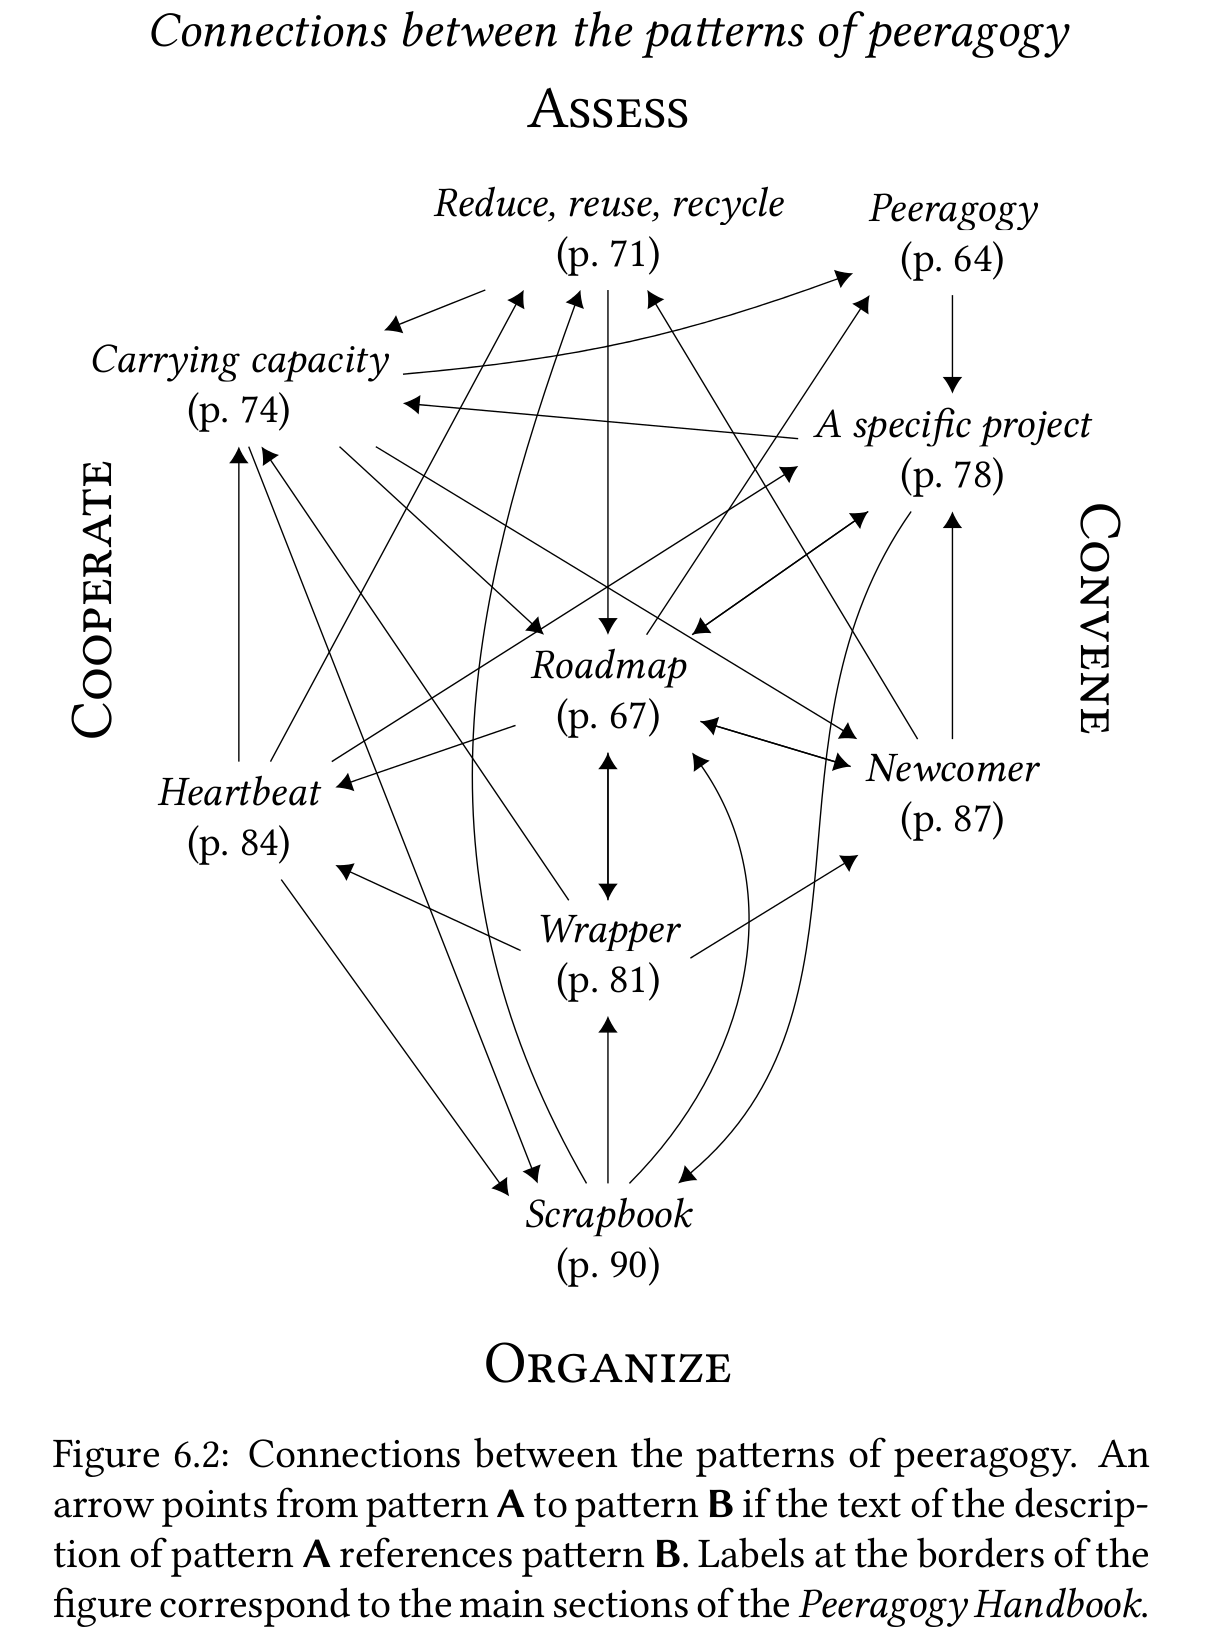
\includegraphics{images/pattern-connections.png}
\caption{image}
\end{figure}

\begin{longtable}[]{@{}l@{}}
\toprule
\begin{minipage}[b]{0.97\columnwidth}\raggedright
overview of problems and solutions in the pattern catalog\strut
\end{minipage}\tabularnewline
\midrule
\endhead
\begin{minipage}[t]{0.97\columnwidth}\raggedright
1. {{Peeragogy}}\strut
\end{minipage}\tabularnewline
\begin{minipage}[t]{0.97\columnwidth}\raggedright
\textbf{How can we find solutions together?} Get concrete about what the
real problems are.\strut
\end{minipage}\tabularnewline
\begin{minipage}[t]{0.97\columnwidth}\raggedright
2. {{Roadmap}}\strut
\end{minipage}\tabularnewline
\begin{minipage}[t]{0.97\columnwidth}\raggedright
\textbf{How can we get everyone on the same page?} Build a plan that we
keep updating as we go along.\strut
\end{minipage}\tabularnewline
\begin{minipage}[t]{0.97\columnwidth}\raggedright
3. {{Reduce, reuse, recycle}}\strut
\end{minipage}\tabularnewline
\begin{minipage}[t]{0.97\columnwidth}\raggedright
\textbf{How can we avoid undue isolation?} Use what's there and share
what we make.\strut
\end{minipage}\tabularnewline
\begin{minipage}[t]{0.97\columnwidth}\raggedright
4. {{Carrying capacity}}\strut
\end{minipage}\tabularnewline
\begin{minipage}[t]{0.97\columnwidth}\raggedright
\textbf{How can we avoid becoming overwhelmed?} Clearly express when
we're frustrated.\strut
\end{minipage}\tabularnewline
\begin{minipage}[t]{0.97\columnwidth}\raggedright
5. {{A specific project}}\strut
\end{minipage}\tabularnewline
\begin{minipage}[t]{0.97\columnwidth}\raggedright
\textbf{How can we avoid becoming perplexed?} Focus on concrete, doable
tasks.\strut
\end{minipage}\tabularnewline
\begin{minipage}[t]{0.97\columnwidth}\raggedright
6. {{Wrapper}}\strut
\end{minipage}\tabularnewline
\begin{minipage}[t]{0.97\columnwidth}\raggedright
\textbf{How can people stay in touch with the project?} Maintain a
summary of activities and any adjustments to the plan.\strut
\end{minipage}\tabularnewline
\begin{minipage}[t]{0.97\columnwidth}\raggedright
7. {{Heartbeat}}\strut
\end{minipage}\tabularnewline
\begin{minipage}[t]{0.97\columnwidth}\raggedright
\textbf{How can we make the project ``real'' for participants?} Keep up
a regular, sustaining rhythm.\strut
\end{minipage}\tabularnewline
\begin{minipage}[t]{0.97\columnwidth}\raggedright
8. {{Newcomer}}\strut
\end{minipage}\tabularnewline
\begin{minipage}[t]{0.97\columnwidth}\raggedright
\textbf{How can we make the project accessible to new people?} Let's
learn together with newcomers.\strut
\end{minipage}\tabularnewline
\begin{minipage}[t]{0.97\columnwidth}\raggedright
9. {{Scrapbook}}\strut
\end{minipage}\tabularnewline
\begin{minipage}[t]{0.97\columnwidth}\raggedright
\textbf{How can we maintain focus as time goes by?} Move things that are
not of immediate use out of focus.\strut
\end{minipage}\tabularnewline
\bottomrule
\end{longtable}

\hypertarget{references}{%
\subsection{References}\label{references}}

\begin{enumerate}
\def\labelenumi{\arabic{enumi}.}
\item
  Christopher Alexander, Sara Ishikawa, and Murray Silverstein. 1977.
  \emph{A Pattern Language: Towns, Buildings, Construction}. Oxford
  University Press, Oxford.
\item
  A.T. Ariyaratne. 1977. Organization of rural communities for group
  effort and self-help. \emph{Food Crisis Workshop, Los Banos, Laguna
  (Philippines), 7-9 Feb 1977}, 23--24. Retrieved from
  \url{http://www.sarvodaya.org/about/philosophy/collected-works-vol-1/rural-self-help}
\item
  Joseph Bergin, Jutta Eckstein, Markus Völter, et al.~2012.
  \emph{Pedagogical patterns: Advice for educators}. Joseph Bergin
  Software Tools, New York.
\item
  James O Coplien and B Woolf. 1997. A pattern language for writers'
  workshops. \emph{C++ report} 9: 51--60.
\item
  J. Corneli and A. Mikroyannidis. 2011. Crowdsourcing Education: A
  Role-Based Analysis. In \emph{Collaborative Learning 2.0: Open
  Educational Resources}, Alexandra Okada, Teresa Connolly and Peter
  Scott (eds.). IGI Global. Retrieved from
  \url{http://oro.open.ac.uk/33221/1/corneli_chap_okada_book.pdf}
\item
  J. Corneli, A. Jordanous, R. Shepperd, et al.~2015. Computational
  Poetry Workshop: Making Sense of Work in Progress. In
  \emph{Proceedings of the Sixth international conference on
  computational creativity, ICCC 2015}, Simon Colton, Hannu Toivonen,
  Michael Cook and Dan Ventura (eds.).
\item
  Joseph Corneli, Dorota Marciniak, Charles Jeffrey Danoff, et al.~2014.
  Building the Peeragogy Accelerator. \emph{Proceedings of OER14:
  Building communities of open practice}. Retrieved from
  \url{http://metameso.org/~joe/docs/Building_the_Peeragogy_Accelerator.pdf}
\item
  Merle Eugene Curti, Vernon Rosco Carstensen, Edmund David Cronon, and
  John William Jenkins. 1949. \emph{The University of Wisconsin, a
  history: 1848-1925}. Univ.~of Wisconsin Press.
\item
  Gilles Deleuze. {[}1968{]} 2004. \emph{Difference and repetition}.
  Bloomsbury Academic, London.
\item
  Neil B Harrison. 1999. The Language of Shepherding. \emph{Pattern
  Languages of Program Design} 5: 507--530.
\item
  Benjamin Mako Hill. 2013. Essays on Volunteer Mobilization in Peer
  Production. Retrieved from
  \url{http://dspace.mit.edu/handle/1721.1/86240}
\item
  Takashi Iba and Iba Laboratory. 2014. \emph{Learning Patterns: A
  Pattern Language for Creative Learning}. CreativeShift Lab, Yokohama.
\item
  Gerard Meszaros and Jim Doble. 1998. A pattern language for pattern
  writing. \emph{Pattern languages of program design} 3: 529--574.
\item
  Marvin Minsky. 1967. Why programming is a good medium for expressing
  poorly understood and sloppily formulated ideas. In \emph{Design and
  Planning II-Computers in Design and Communication}. 120--125.
\item
  PLAST Collective. 2015. The PLAST Project: Pattern Languages for
  Systemic Transformation. \emph{Spanda Journal} VI, 1: 205--218.
\item
  René Reiners, Ragnhild Halvorsrud, Aslak Wegner Eide, and Daniela
  Pohl. 2012. An approach to evolutionary design pattern engineering.
  \emph{Proceedings of the 19th Conference on Pattern Languages of
  Programs}.
\item
  Douglas Schuler. 2008. \emph{Liberating voices: A pattern language for
  communication revolution}. MIT Press, Cambridge, MA.
\item
  Till Schümmer, Joerg M Haake, and Wolfgang Stark. 2014. Beyond
  rational design patterns. \emph{Proceedings of the 19th european
  conference on pattern languages of programs}, ACM, 13 pp.
\item
  Booker T Washington. 1901. \emph{Up from slavery}. Doubleday \&
  Company, Inc.
\end{enumerate}

\begin{center}\rule{0.5\linewidth}{0.5pt}\end{center}



\chapter{Emergent Roadmap} \label{sec:Distributed_Roadmap}
\hypertarget{emergent-roadmap}{%
\section{Emergent Roadmap}\label{emergent-roadmap}}

\begin{quote}
This section reprises the ``What's Next'' steps in all the previous
patterns, offering another view on the project \textbf{Roadmap} in its
emergent form.
\end{quote}

\hypertarget{peeragogy}{%
\subsubsection{▶ Peeragogy}\label{peeragogy}}

We intend to revise and extend the patterns and methods of peeragogy to
make it a workable model for learning, inside or outside of
institutions.

\hypertarget{roadmap}{%
\subsubsection{▶ Roadmap}\label{roadmap}}

If we sense that something needs to change about the project, that is a
clue that we might need to record a new pattern, or revise our existing
patterns.

\hypertarget{reduce-reuse-recycle}{%
\subsubsection{▶ Reduce, reuse, recycle}\label{reduce-reuse-recycle}}

We've converted our old pattern catalog from the \emph{Peeragogy
Handbook} into this paper, sharing it with a new community and gaining
new perspectives. Can we repeat that for other things we've made?

\hypertarget{carrying-capacity}{%
\subsubsection{▶ Carrying capacity}\label{carrying-capacity}}

Making it easy and fruitful for others to get involved is one of the
best ways to redistribute the load. This often requires skill
development among those involved; compare the pattern.

\hypertarget{a-specific-project}{%
\subsubsection{▶ A specific project}\label{a-specific-project}}

We need to build specific, tangible ``what's next'' steps and connect
them with concrete action. Use the Scrapbook to organize that process.

\hypertarget{wrapper}{%
\subsubsection{▶ Wrapper}\label{wrapper}}

We have prototyped and deployed a visual ``dashboard'' that people can
use to get involved with the ongoing work in the project. Let's improve
it, and match it with an improved interaction design for peeragogy.org.

\hypertarget{heartbeat}{%
\subsubsection{▶ Heartbeat}\label{heartbeat}}

Identifying and fostering new and new working groups is a task that can
help make the community more robust. This is the time dimension of spin
off projects described in Reduce, reuse, recycle.

\hypertarget{newcomer}{%
\subsubsection{▶ Newcomer}\label{newcomer}}

A more detailed (but non-limiting) ``How to Get Involved'' walk-through
or ``DIY Toolkit'' would be good to develop. We can start by listing
some of the things we're currently learning about.

\hypertarget{scrapbook}{%
\subsubsection{▶ Scrapbook}\label{scrapbook}}

After pruning back our pattern catalog, we want it to grow again: new
patterns are needed. One strategy would be to ``patternize'' the rest of
the \emph{Peeragogy Handbook.}
 

\renewcommand*{\footnote}[1]{\oldfootnote{#1}}%
\renewcommand*{\textsuperscript}[1]{\oldtextsuperscript{#1}}%

\chapter{Case Study: SWATs} \label{swats}
\begin{quote}
Learning to use technology with peers -- the case of Students With
Abilities in Technology (SWATs).
\end{quote}

\hypertarget{part-1-introduction}{%
\subsection{Part 1: Introduction}\label{part-1-introduction}}

Mind-amplifying technologies {{[}1{]}}, technologies of cooperation
{{[}2{]}}, such as conversation technologies, as well as visualization
tools, video and photo edition software, simulators or programming
technologies are emerging learning tools in schools around the world.
They are affordable and accessible enough to design learning
environments. Latin America is no exception and it is fast becoming the
norm to find convergent technology in the classroom.

We challenged students to develop a three-level game with a score or
marker using Scratch, a program developed by MIT. This program allows
you to develop computer programs using modules or blocks of
instructions. The educational value of this tool lies not in its ease of
use but in its nature as an authentic learning environment and ideal
context for developing intellectual skills.

Once students have developed their programs and documented the process
in a learning log, we asked them if they had faced problems in handling
Scratch. In this way we were able to identify which students had
difficulties in developing programs and what their problems were in the
process of choosing instructions. ~However, we're also able to identify
those students with particular technical skills. ~We call them Students
With Abilities in Technology (SWATs). ~In case of difficulty, SWATs can
be called in, and can decide if they want to give advice to peers and
the teacher in the use of Scratch.

The idea of identifying these students and asking them to support their
peers and teachers in specific tasks has an additional educational
component. It is clear that when a student is given the task of
explaining or advising peers or teachers, he develops new competences
and masters, to an even greater extent, those competences for which
he/she was selected as SWAT.

We have observationally determined that this approach is relevant to the
widespread use of digital devices in academic tasks and its extended
application contributes to a more positive use of digital technologies
for learning. We see how, as the use of technology in all learning
environments becomes general, this approach of peer learning becomes an
alternative to underpin the work of teachers. The figure of the SWAT in
the classroom also enables a different form of relationship between
pairs that generate new forms of interaction and learning that we can
appraise and evaluate.

\hypertarget{part-2.-representation-as-a-pattern}{%
\subsection{Part 2. Representation as a
pattern}\label{part-2.-representation-as-a-pattern}}

Here's how the above case could be described using the pattern template
that we've presented in the book. ~This may help others use the same
model --- or at least understand how it works in practice in more
detail. ~Further questions may come to mind, which the reader can try to
answer by transforming or extending the pattern in their own context.

\hypertarget{title}{%
\paragraph{Title:}\label{title}}

Students With Abilities in Technology (SWAT)

\hypertarget{definition}{%
\paragraph{Definition:}\label{definition}}

Private and public schools increasingly have digital devices in
classrooms with Internet access (laptops, desktops, tablets, cell
phones, etc.) and teachers with little or no expertise in the
educational use of such devices. ~However, some of the students have
considerable background with these kinds of tools.~ They can help the
teachers and other students.

\hypertarget{problem}{%
\paragraph{Problem:}\label{problem}}

In general, teachers have multiple deficiencies in the adoption of
emerging technologies. Their lack of expertise prevents them from
realizing the full potential that technology has as a relevant
pedagogical mediation. ~The rate of change in the school context,
however, is not coupled to the rate of change in ~current teacher
training programs. This lack of pedagogical training is having a majorly
disruptive impact in the classroom given this presence of technological
devices in the classroom. ~The reaction of administrators and teachers
to the proliferation of devices is, in a significant number of cases,
rejection and stigmatization of emerging technologies. The cause of this
rejection is that teachers ignore the educational potential of
technology. They ignore how technology has changed the cognitive model
of a whole generation. ~Having technical specialists to support the work
of the teacher in the classroom is unthinkable from an economic
standpoint.

\hypertarget{solution}{%
\paragraph{Solution:}\label{solution}}

The students themselves can be the solution to this problem. Some have
superior technical knowledge and this is usually wasted. Teachers can
incorporate them as assistants to help them and their peers. A student
with digital skills can be the agent of change that many teachers need
in order to learn how to use technology for the design of learning
environments. ~This empowered group of students, that we named SWAT
(Students With Abilities in Technology) support teachers and peers with
lower-level digital competences. Support from students with technical
knowledge could mean a significant change in the learning process,
because teachers can now combine that knowledge with their teaching
experience and pedagogical strategies. The result of this can be the
discovery of the many possibilities technology has for the construction
of knowledge and the development of new intellectual abilities.

In our work with middle school students (ages 12-14), the support of
SWATs inside and outside the classroom was a very positive experience.
At the beginning of each course students are required to develop
projects involving the use of technology. Students who show a greater
competence in the use of technical tools are invited to join as SWAT.
Once SWATs are identified, they are asked about the possibility of
supporting teachers and their peers in the use of specific computer
tools. It is impressive to see teachers becoming co-learners who take
advantage of this privileged status of their students to master tools
that promote their ability to redesign learning environments. ~When
students need support for developing their projects, SWATs show them
strategies to accomplish them. The majority report great pleasure and
pride in their new role as peer advisors.

\hypertarget{challenges-arising-in-practice}{%
\paragraph{Challenges arising in
practice:}\label{challenges-arising-in-practice}}

This peeragogical approach changes the prevailing educational paradigm
through collaboration between teachers and students, and among students
themselves. ~There are many possible points of friction. ~To have one or
more SWATs in each learning group transforms the way in which teachers
and students interact with each other and with available technologies,
but, again, can create challenges for teachers who may be used to a more
``banking'' style of teaching.

\hypertarget{whats-next}{%
\paragraph{What's next:}\label{whats-next}}

Can we find mentors for the SWATs to help them become even better with
technology? ~Can we find other ways to reward these students? ~At the
same time, can the idea be applied across the curriculum, and across
other competencies, to involve more students in the peer-teaching role?

\hypertarget{references}{%
\subsection{References}\label{references}}

\begin{enumerate}
\def\labelenumi{\arabic{enumi}.}
\item
  Howard Rheingold (2012), ``Mind Amplifier: Can Our Digital Tools Make
  Us Smarter?''
\item
  Institute of the Future (2005),
  ``\href{http://www.rheingold.com/cooperation/Technology_of_cooperation.pdf}{Technology
  of cooperation}.''
\end{enumerate}


\part{~Convening A Group} \label{convening-part} %%%%%%%%%%%%%%%%%%%%
%
\chapter[\textbf{So you've decided to try peer learning\ldots}]{So you've decided to try peer learning\ldots}
\begin{quote}
So you've decided to try peer learning? Maybe you've already found a few
people who will support you in this effort. Congratulations! It's time
now to focus your thinking. How will you convene others to form a
suitable group? How will you design a learner experience which will make
your project thrive? In this chapter, we suggest a variety of questions
that will help you to make your project more concrete for potential new
members. There are no good or bad answers - it depends on the nature of
your project and the context. Trying to answer the questions is not
something you do just once. At various stages of the project, even after
it's over, some or all of those questions will aquire new meanings - and
probably new answers.
\end{quote}

\begin{quote}
\textbf{Fabrizio Terzi}: ``There is a force of attraction that allows
aggregation into groups based on the degree of personal interest; the
ability to enhance and improve the share of each participant; the
expectation of success and potential benefit.''
\end{quote}

\hypertarget{group-identity}{%
\subsection{Group identity}\label{group-identity}}

Note that there are many groups that may not need to be ``convened'',
since they already exist. There is a good story from
\href{http://www.sarvodayausa.org/learn/a-t-ariyartne/}{A. T.
Ariyaratne} in his
\href{http://www.sarvodaya.org/about/philosophy/collected-works-vol-1/rural-self-help}{collected
works} in which he does ``convene'' a natural group (a village) - but in
any case, keep in mind at the outset that the degree of
group-consciousness that is necessary for peer learning to take place is
not fixed. In this section, we suppose you are just at the point of
kicking off a project. What steps should you take? We suggest you take a
moment to ponder the following questions first - and revisit them
afterward, as a way to identify best practices for the next effort.

\hypertarget{there-will-be-a-quiz}{%
\subsection{There will be a quiz}\label{there-will-be-a-quiz}}

Those taking the initiative should ask themselves the traditional Who,
What, Where, When, Why, and How.
(\href{http://en.wikipedia.org/wiki/Simon_Sinek}{Simon Sinek} suggests
to begin with Why, and we touched on Who, above!). In doing so,
preliminary assumptions for design and structure are established.
However, in peer learning it is particularly important to maintain a
healthy degree of openness, so that future group members can also form
their answers on those questions. In particular, this suggests that the
design and structure of the project (and the group) may change over
time. Here, we riff on the traditional 5W's+H with six clusters of
questions to~help you focus your thinking about the project and amplify
its positive outcomes.

\hypertarget{expectations-for-participants}{%
\subsection{Expectations for
participants}\label{expectations-for-participants}}

\textbf{1. Who: Roles and flux}

\begin{itemize}
\tightlist
\item
  What are some of the roles that people are likely to fall into (e.g.
  Newcomer, Wrapper, Lurker, Aggregator, etc.)?
\item
  How likely is it that participants will stick with the project? If you
  expect many participants to leave, how will this effect the group and
  the outcome?
\item
  Do you envision new people joining the group as time goes by? If so,
  what features are you designing that will support their integration
  into an existing flow?
\item
  Will the project work if people dip in and out? If so, what features
  support that? If not, how will people stay focused?
\end{itemize}

\textbf{2. What: Nature of the project}

\begin{itemize}
\tightlist
\item
  What skills are required? What skills are you trying to build?
\item
  What kinds of change will participants undergo? Will they be heading
  into new ground? Changing their minds about something? Learning about
  learning?
\item
  What social objective, or ``product'' if any, is the project aiming to
  achieve?
\item
  What's the `hook?'~Unless you are working with an existing group, or
  re-using an existing modality, consistent participation may not be a
  given.
\end{itemize}

\textbf{3. When: Time management}

\begin{itemize}
\tightlist
\item
  What do you expect the group to do, from the moment it convenes, to
  the end of its life-span, to create the specific outcome that will
  exist at the conclusion of its last meeting? {[}2{]} Note that what
  people ACTUALLY do may be different from what you envision at the
  outset, so you may want to revisit this question (and your answer)
  again as the project progresses.
\item
  Keeping in mind that at least one period of is inertia is very likely
  {[}2{]}, what event(s) do you anticipate happening in the group that
  will bring things back together, set a new direction, or generally get
  things on track? More generally, what kinds of contingencies does your
  group face? How does it interface to the ``outside world''?
\item
  What pre-existing narratives or workflows could you copy in your
  group?
\item
  How much of a time commitment do you expect from participants? Is this
  kind of commitment realistic for members of your group?
\item
  What, if anything, can you do to make participation ``easy'' in the
  sense that it happens in the natural flow of life for group members?
\item
  Does everyone need to participate equally? How might non-equal
  participation play out for participants down the line?
\end{itemize}

\textbf{4. Where: Journey vs Destination}

\begin{itemize}
\tightlist
\item
  What structures will support participants in their journey to the end
  result(s) you (or they) have envisioned? What content can you use to
  flesh out this structure?
\item
  Where can the structure ``flex'' to accommodate unknown developments
  or needs as participants learn, discover, and progress?
\end{itemize}

\textbf{5. Why: Tool/platform choice}

\begin{itemize}
\tightlist
\item
  What tools are particularly suited to this group? Consider such
  features as learning styles and experiences, geographical diversity,
  the need for centralization (or de-centralization), cultural
  expectations related to group work, sharing, and emerging leadership.
\item
  Is there an inherent draw to this project for a given population, or
  are you as facilitator going to have to work at keeping people
  involved? How might your answer influence your choice of tools? Is the
  reward for completion the learning itself, or something more tangible?
\item
  In choosing tools, how do you prioritize such values and objectives as
  easy entry, diverse uses, and high ceilings for sophisticated
  expansion?
\end{itemize}

\textbf{6. How: Linearity vs Messiness}

\begin{itemize}
\tightlist
\item
  How will your group manage feedback in a constructive way?
\item
  Why might participants feel motivated to give feedback?
\item
  How firm and extensive are the social contracts for this group? Do
  they apply to everyone equally, or do they vary with participation
  level?
\item
  What do people need to know at the start? What can you work out as you
  go along? Who decides?
\item
  How welcome are ``meta-discussions''? What kinds of discussions are
  not likely to be welcome? Do you have facilities in place for
  ``breakout groups'' or other peer-to-peer interactions?
  (Alternatively, if the project is mostly distributed, do you have any
  facilities in place for coming together as a group?)
\end{itemize}

\hypertarget{cycles-of-group-development}{%
\subsection{Cycles of group
development}\label{cycles-of-group-development}}

The above questions remain important thoughout the life of the project.
People may come and go, particpants may propose fundamentally new
approaches, people may evolve from lurkers to major content creators or
vice-versa. The questions we suggest can be most effective if your group
discusses them over time, as part of its workflow, using synchronous
online meetings (e.g., \href{http://www.bigbluebutton.org/}{Big Blue
Button},
\href{http://success.adobe.com/en/na/sem/products/connect/1109_6011_connect_webinars.html?sdid=IEASO\&skwcid=TC/textbar\%7B\%7D22191/textbar\%7B\%7Dadobe\%20connect/textbar\%7B\%7D/textbar\%7B\%7DS/textbar\%7B\%7De/textbar\%7B\%7D5894715262}{Adobe
Connect},
\href{http://www.blackboard.com/platforms/collaborate/overview.aspx}{Blackboard
Collaborate}), forums, Google docs, wikis, and/or email lists. Regular
meetings are one way to establish a ``heartbeat'' for the group.

In thinking about other ways of structuring things, note that the
``body'' of the \emph{Peeragogy Handbook} follows a
\href{http://en.wikipedia.org/wiki/Forming-storming-norming-performing}{Tuckman-like
outline} (\emph{Convening a Group} is our ``forming'', \emph{Organizing
a Learning Context} is our ``storming and norming'',
\emph{Co-working/Facilitation} is our ``performing'', and
\emph{Assessment} is our ``adjourning''). But we agree with Gersick
{{[}1{]}}, and Engeström {{[}2{]}}, that groups do not always follow a
linear or cyclical pattern with their activities!

Nevertheless, there may be some specific stages or phases that you want
\emph{your} group to go through. Do you need some ``milestones,'' for
example? How will you know when you've achieved ``success?''

In closing, it is worth reminding you that it is natural for groups to
experience conflict, especially as they grow or cross other threshold
points or milestones - or perhaps more likely, when they don't cross
important milestones in a timely fashion (ah, so you remember those
milestones from the previous section!). Nevertheless, there are some
strategies can be used to make this conflict productive, rather than
merely destructive (see Ozturk and Simsek {{[}3{]}}).

\hypertarget{references}{%
\subsection{References}\label{references}}

\begin{enumerate}
\def\labelenumi{\arabic{enumi}.}
\item
  Gersick, C. (1988). Time and transition in work teams: Toward a new
  model of group development. \emph{Academy of Management Journal} 31
  (Oct.): 9-41.
\item
  Engeström, Y. (1999). Innovative learning in work teams: Analyzing
  cycles of knowledge creation in practice. In Y. Engeström, R.
  Miettinen \& R.-L-. Punamäki (Eds.), \emph{Perspectives on activity
  theory}, (pp.~377-404). Cambridge, UK: Cambridge University Press.
\item
  Ozturk and Simsek (2012). ``Of Conflict in Virtual Learning
  Communities in the Context of a Democratic Pedagogy: A paradox or
  sophism?,'' in \emph{Proceedings of the Networked Learning Conference,
  2012, Maastricht.}
  (\href{http://www.lancaster.ac.uk/fass/edres/seminars/Ozturk300311.htm}{Video}
  or
  \href{http://networkedlearningconference.org.uk/abstracts/pdf/ozturk.pdf}{text.})
\end{enumerate}

%
\chapter[\textbf{Play and learning}]{Play and learning}
%
Once more we're back to the question, ``What makes learning fun?'' There
are deep links between play and learning. Consider, for instance, the
way we learn the rules of a game through playing it. The first times we
play a card game, or a physical sport, or a computer simulation we test
out rule boundaries as well as our understanding. Actors and
role-players learn their roles through the dynamic process of
performance. The resulting learning isn't absorbed all at once, but
accretes over time through an emergent process, one unfolding further
through iterations. In other words, the more we play a game, the more we
learn it.

In addition to the rules of play, we learn about the subject which play
represents, be it a strategy game (chess, for example) or simulation of
economic conflict. Good games echo good teaching practice, too, in that
they structure a single player's experience to fit their regime of
competence (cf.~Vygotsky's zone of proximal learning, a la Gee
{{[}1{]}}). That is to say a game challenges players at a level suited
to their skill and knowledge: comfortable enough that play is possible,
but so challenging as to avoid boredom, eliciting player growth.
Role-playing in theater lets performers explore and test out concepts;
see Boal {{[}2{]}}. Further, adopting a playful attitude helps
individuals meet new challenges with curiousity, along with a readiness
to mobilize ideas and practical knowledge. Indeed, the energy activated
by play can take a person beyond an event's formal limitations, as
players can assume that play can go on and on {{[}3{]}}.

\begin{quote}
\textbf{Douglas Thomas and John Seely Brown}: ``All systems of play are,
at base, learning systems.'' {{[}4{]}}
\end{quote}

Games have always had a major social component, and learning plays a key
role in that interpersonal function. Using games to build group cohesion
is an old practice, actually a triusm in team sports.

It is important to locate our peeragogical moment in a world where
gaming is undergoing a renaissance. Not only has digital gaming become a
large industry, but gaming has begun to infiltrate non-gaming aspects of
the world, sometimes referred to as ``gamification.'' Putting all three
of these levels together, we see that we can possibly improve
co-learning by adopting a playful mindset. Such a playful attitude can
then mobilize any or all of the above advantages. For example,

\begin{itemize}
\tightlist
\item
  Two friends are learning the Russian language together. They invent a
  vocabulary game: one identifies an object in the world, and the other
  must name it in Russian. They take turns, each challenging the other,
  building up their common knowledge.
\item
  A middle-aged man decides to take up hiking. The prospect is somewhat
  daunting, since he's a very proud person and is easily stymied by
  learning something from scratch. So he adopts a ``trail name'', a
  playful pseudonym. This new identity lets him set-aside his
  self-importance and risk making mistakes. Gradually he grows
  comfortable with what his new persona learns.
\item
  We can also consider the \textbf{design} field as a useful kind of
  playful peeragogy. The person \emph{playing the role} of the designer
  can select the contextual frame within which the design is performed.
  This frame can be seen as the \emph{rules} governing the design, the
  artifact and the process. These rules, as with some games, may change
  over time. Therefore the possibility to adapt, to tailor one's
  activities to changing context is important when designing playful
  learning activities. (And we'll look at some ways to design peer
  learning experiences next!)
\end{itemize}

Of course, ``game-based learning'' can be part of standard pedagogy too.
When peers create the game themselves, this presumably involves both
game-based learning and peer learning. Classic strategy games like
\href{http://senseis.xmp.net/?MythOfOrigin}{Go} and
\href{http://www.amazon.com/Chess-Success-Using-Strengths-Children/dp/0767915682}{Chess}
also provide clear examples of peer learning practices: the question is
partly, what skills and mindsets do our game-related practices really
teach?

\begin{quote}
\textbf{Socrates}: ``No compulsory learning can remain in the soul
\ldots In teaching children, train them by a kind of game, and you will
be able to see more clearly the natural bent of each.''
\end{quote}

\hypertarget{exercises-that-can-help-you-cultivate-a-playful-attitude}{%
\subsection{Exercises that can help you cultivate a playful
attitude}\label{exercises-that-can-help-you-cultivate-a-playful-attitude}}

\begin{itemize}
\tightlist
\item
  Use the \href{http://www.rtqe.net/ObliqueStrategies/}{Oblique
  Strategies} card deck (Brian Eno and Peter Schmidt, 1st edition 1975,
  now available in its fifth edition) to spur playful creativity. Each
  card advises players to change their creative process, often in
  surprising directions.
\item
  Take turns making and sharing videos. This online collaborative
  continuous video storytelling involves a group of people creating
  short videos, uploading them to YouTube, then making playlists of
  results. Similar to \href{http://clipkino.info/}{Clip Kino}, only
  online.
\item
  Engage in theater play using Google+ Hangout. e.g.~coming together
  with a group of people online and performing theatrical performances
  on a shared topic that are recorded.
\end{itemize}

\hypertarget{references}{%
\subsection{References}\label{references}}

\begin{enumerate}
\def\labelenumi{\arabic{enumi}.}
\item
  Gee, J. P. (1992). \emph{The social mind: Language, ideology, and
  social practice}. Series in language and ideology. New York: Bergin \&
  Garvey.
\item
  Boal, A. (1979). \emph{Theatre of the oppressed}. 3rd ed.~London:
  Pluto Press.
\item
  Bereiter, C. and Scadamalia, M. (1993). \emph{Surpassing ourselves, an
  inquiry into the nature and implications of expertise}. Peru,
  Illinois: Open Court.
\item
  Douglas Thomas and John Seely Brown (2011), \emph{A New Culture of
  Learning: Cultivating the Imagination for a World of Constant Change}.
  CreateSpace.
\item
  Malone, T.W. (1981), Toward a Theory of Intrinsically Motivating
  Instruction, \emph{Cognitive Science}, 4, pp.~333-369
\end{enumerate}

%
\chapter[\textbf{K-12 Peeragogy}]{K-12 Peeragogy}
%
Teachers tend to work in isolation on their own islands, keeping their
learning to themselves, yet they also generously share resources with
one another. It is this latter trait that is becoming increasingly
important as the role of the educator continues to expand. As
educational technology research specialist Stephen Downes
\href{http://www.huffingtonpost.com/stephen-downes/the-role-of-the-educator_b_790937.html}{observes},
the expectations on teachers have grown from ``being expert in the
discipline of teaching and pedagogy\ldots{}{{[}to needing to have{]}}
up-to-date and relevant knowledge and experience in it. Even a teacher
of basic disciplines such as science, history or mathematics must remain
grounded, as no discipline has remained stable for very long, and all
disciplines require a deeper insight in order to be taught
effectively.'' It is no longer possible for an educator to work alone to
fulfil each of these roles: the solution is to work and learn in
collaboration with others. This is where peer-based sharing and learning
online, connected/networked learning, or peeragogy, can play an
important role in helping educators.

\hypertarget{becoming-a-connectednetworked-learner}{%
\subsection{Becoming a connected/networked
learner}\label{becoming-a-connectednetworked-learner}}

The following steps are set out in `phases' in order to suggest possible
experiences one may encounter when becoming connected. It is
acknowledged that every learner is different and these `phases' only
serve as a guide.

\hypertarget{phase-1-deciding-to-take-the-plunge}{%
\subsection{Phase 1: Deciding to take the
plunge}\label{phase-1-deciding-to-take-the-plunge}}

To help educators begin to connect, the
\href{http://www.google.com/url?q=https\%3A\%2F\%2Fdl.dropbox.com\%2Fu\%2F38904447\%2Fstarter-kit-final.pdf\&sa=D\&sntz=1\&usg=AFQjCNE9sNo1Lz9-zJ0KH48djXeYVoAF4A}{Connected
Educator's Starter Kit} was created during Connected Educator's Month in
August 2012. This chapter previews the main steps. The first step to
becoming a `connected educator-learner' involves making the commitment
to spending the time you'll need to learn how to learn and share in an
open, connected environment.

\hypertarget{phase-2-lurking}{%
\subsection{Phase 2: Lurking}\label{phase-2-lurking}}

We start off as lurkers. A learner can be considered a true `lurker'
after reviewing the starter kit, establishing a digital presence
(through a blog or a wiki) or signing up for Twitter and creating a
basic profile containing a photo. In this phase, lurkers will begin to
\href{http://www.google.com/url?q=http\%3A\%2F\%2Fwww.fractuslearning.com\%2F2012\%2F05\%2F25\%2Ftwitter-follow-education-technology\%2F\&sa=D\&sntz=1\&usg=AFQjCNF8grPMuRwU_ImW9Jk3ZYrg0m9KgQ}{`follow'
other users on Twitter} and observe
\href{http://www.google.com/url?q=http\%3A\%2F\%2Fcybraryman.com\%2Fchats.html\&sa=D\&sntz=1\&usg=AFQjCNFJASZiwfvPbfOzFbHvAunpXfNC1g}{educational
Twitter `chats'}. Lurkers will also begin to seek out other resources
through
\href{http://theinnovativeeducator.blogspot.ca/2012/04/ten-best-education-blogs.html}{blogs},
\href{http://www.google.com/url?q=http\%3A\%2F\%2Fwww.edsocialmedia.com\%2F2011\%2F02\%2Fthe-advantage-of-facebook-groups-in-education\%2F\&sa=D\&sntz=1\&usg=AFQjCNEvc43Q7GqJqS-2S8GhEJ53Ye-j4Q}{Facebook},
\href{http://www.slideshare.net/cmsdsquires/edmodo-for-teachers-guide}{Edmodo}
and
\href{http://www.emergingedtech.com/2012/02/8-great-linkedin-groups-for-educators/}{LinkedIn}
groups.

\hypertarget{phase-3-entering-the-fray}{%
\subsection{Phase 3: Entering the
fray}\label{phase-3-entering-the-fray}}

The lurker begins to develop into a connected educator-learner once he
or she makes the decision to enter into a dialogue with another user.
This could take the form of a personal blog post, participation on an
education-related
\href{http://edudemic.com/2012/08/education-blogs/?utm_medium=twitter\&utm_source=twitterfeed}{blog}
or
\href{http://educationalwikis.wikispaces.com/Examples+of+educational+wikis}{wiki}
or an exchange with another Twitter user. Once this exchange takes
place, relationships may begin to form and the work towards building a
Personal Learning Network (PLN) begins.

One such site where such relationships can be built is
\href{http://www.classroom20.com/}{Classroom 2.0}, which was founded by
\href{http://www.stevehargadon.com/}{Steve Hargadon.} Through Classroom
2.0, Steve facilitates a number of free online learning opportunities
including weekly
\href{http://www.google.com/url?q=http\%3A\%2F\%2Fwww.futureofeducation.com\%2Fnotes\%2FPast_Interviews\&sa=D\&sntz=1\&usg=AFQjCNHVYOvP-w7NTgKp2Fu2AX4YycnPQQ}{Blackboard
Collaborate} sessions, conferences, book projects and grassroots
cross-country educational-transformation tours. Classroom 2.0 also
offers a supportive Social Ning---a free, social learning space that
provides online conferences and synchronous and recorded interviews with
inspirational educators---for connected educator-learners around the
world.

\hypertarget{phase-4-building-and-shaping-your-pln}{%
\subsection{Phase 4: Building and shaping your
PLN}\label{phase-4-building-and-shaping-your-pln}}

Just as not every person one meets becomes a friend, it is important to
remember that not every exchange will lead to a co-learning peeragogy
arrangement. It may be sufficient to follow another who provides useful
content without expecting any reciprocation. It is dependent on each
educator-learner to determine who to pay attention to and what learning
purpose that individual or group will serve. It is also up to the
learner-educator to demonstrate to others that he or she will actively
participate.

There are a number of
\href{http://storify.com/digiphile/how-to-build-a-personal-learning-network-on-twitte}{strategies}
one can use when shaping the PLN to learn. However, one of the best ways
educators can attract a core of \emph{peeragogues} is by sharing
actively and demonstrating active and open learning for others.

There are a number of sites where a new educator-learner can actively
and openly learn. In addition to personal blogging and wikis, other
professional development opportunities include open, online courses and
weekly synchronous online meetings through video, podcasts or other
forms of media.

Examples include:
\href{http://connectedlearning.tv/howard-rheingold-social-media-and-peer-learning-mediated-pedagogy-peeragogy}{Connected
Learning TV},
\href{http://techtalktuesdays.global2.vic.edu.au/}{TechTalkTuesdays},
\href{http://learning2gether.pbworks.com/w/page/32206114/volunteersneeded}{VolunteersNeeded},
\href{http://simplek12.com/webinars}{SimpleK12},
\href{http://k12onlineconference.org/}{K12 Online,}
\href{http://www.learnnowbc.ca/educators/moodlemeets/default.aspx}{CEET},
and \href{http://edtechtalk.com/taxonomy/term/130}{EdTechTalk}.

Alternatively, courses are offered with
\href{https://p2pu.org/en/schools/school-of-ed-pilot/}{P2PU's} School of
Education or a wide variety of other opportunities collected by
\href{http://www.teachthought.com/}{TeachThought} and Educator's CPD
online. Peggy George, the co-faciliator of the weekly Classroom 2.0 LIVE
Sessions, created a livebinder package of free
`\href{http://www.google.com/url?q=http\%3A\%2F\%2Fwww.livebinders.com\%2Fplay\%2Fplay_or_edit\%3Fid\%3D429095\&sa=D\&sntz=1\&usg=AFQjCNHCIdRn64rPwske2vP7xrpWolb-jA}{PD
On Demand}' connected professional development online options for
peeragogy enthusiasts.

\hypertarget{phase-5-extending-the-digital-pln-and-connecting-face-to-face}{%
\subsection{Phase 5: Extending the digital PLN and connecting
face-to-face}\label{phase-5-extending-the-digital-pln-and-connecting-face-to-face}}

Over time, once the connected educator-learner has established a refined
PLN, these peeragogues may choose to shift their learning into physical
learning spaces. Some options available for these educator-learners
would include the new `grassroots unconferences', which include examples
such as: \href{http://educonphilly.org/}{EduCon},
\href{http://davidwees.com/content/what-edcamp}{EdCamps},
\href{http://thatcamp.org/}{THATcamp} and
\href{http://connectedcanada.org/}{ConnectedCA}.

These (un)conferences are free or extremely low-cost and focus on
learning from and with others. These `unconferences' are typically
publicized through Twitter, Google Apps, and Facebook. Connecting
face-to-face with other peeragogues can strengthen bonds to learning
networks and help to promote their sustainability.

\hypertarget{postscript}{%
\subsection{Postscript}\label{postscript}}

Sylvia Tolisano, Rodd Lucier and Zoe Branigan-Pipen co-created an
\href{http://farm9.staticflickr.com/8160/7161689001_9b6725a4ca_h.jpg}{infographic}
which explores the experiences individuals may encounter in the journey
to become connected learners through another related sequence of steps:
\emph{Lurker}, \emph{Novice}, \emph{Insider}, \emph{Colleague},
\emph{Collaborator}, \emph{Friend}, and \emph{Confidant}. Googlize it,
and have a look at our
\href{http://peeragogy.org/recommended-reading/}{Recommended Readings}
in Chapter 31 for additional resources.

%
\chapter[\textbf{P2P SOLE}]{P2P Self-Organized Learning Environments}
%
\begin{quote}
This conversational piece invites you to engage in a journey to create
your own learning space. You'll find many points of entry that allow you
to affectd emerging structure. Reciprocal mentoring can create a ripple
effect for those who follow.
\end{quote}

\subsection{The Guiding Strategy:}\label{the-guiding-strategy}

In his \href{http://peeragogy.org/case-study-5ph1nx/}{Peeragogical Case
Study} David Preston states:

\begin{quote}
\emph{Peeragogical interaction requires refining relational and topical
critique, as well as skills in other ``meta'' literacies, including but
not limited to critical thinking, collaboration, conflict resolution,
decision-making, mindfulness, patience and compassion.}
\end{quote}

A
\href{http://en.wikipedia.org/wiki/Self_Organised_Learning_Environment}{Self-Organizing
Learning Environment}, or SOLE, with a living structure accomplishes all
of these outcomes, or David's ``meta-literacies,'' simultaneously. An
authentic problem and/or project based activity in a connected learning
environment includes diverse learners in diverse ways by empowering all
learners as peers.

This provides the authentic learning environment with which to design a
SOLE. SOLEs are everywhere. How have we evolved as a species, if not
through self-organizing? A conversation between strangers is self
organizing, each learning about something or each other. The spaces
around people conversing is also an environment, though not explicitly a
learning one. 

While we are always self-organizing to learn or accomplish

\clearpage
\begin{vplace}[0.5]
\noindent 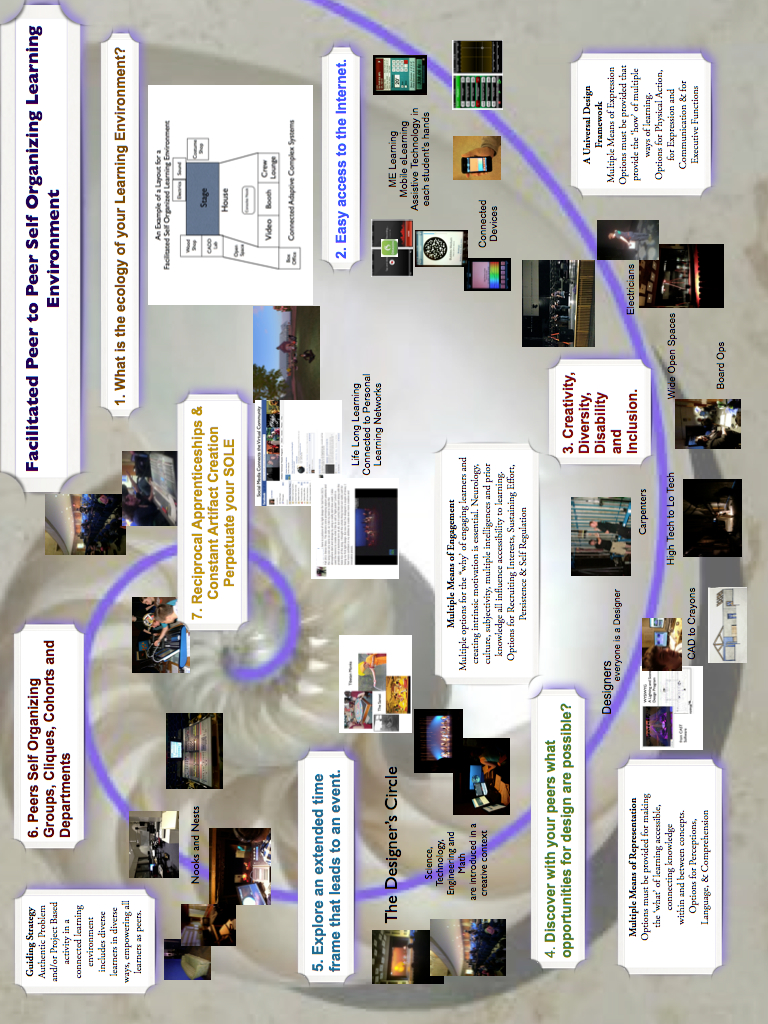
\includegraphics[width=\textwidth]{../pictures/sole-l.jpg}
A visualization of the facilitated peer to peer SOLE, full-size
at \url{http://goo.gl/7StkJK}
\end{vplace}
\clearpage

\noindent things, one place that SOLEs do not always exist are in
learning institutions. In many educational institutions, our learning
environments are predominately organized by the teacher, curriculum,
or society. How can we nurture peer to peer learning environments to
organize? How does the role of the teacher differ in a SOLE? In what
ways can we unite that fundamental, passionate human characteristic of
curiosity and self-organizing back into our Learning Environments?

The model that \href{http://sugatam.wikispaces.com/}{Sugata Mitra}
{{[}2{]}} is experimenting with gives us some scaffolding to create one
ourselves. This is the goal of his
\href{http://www.ted.com/pages/sole_toolkit}{SOLE Tool Kit} (3).
Sugata's kit is directed towards children between 8 and 12 years old. I
was wondering if there is a way to make it more universal in its
application. How can I apply it to my situation? How is a SOLE different
in the context of peer to peer learning? This chapter of the Handbook
uses Sugata's model as a doorway into our understanding a SOLE approach
to peer to peer learning. Its three key components are: learners,
context and project. I find the discussion needs to integrate what we
are learning about diverse learners into a
\href{http://www.udlcenter.org/aboutudl/udlguidelines}{Universal Design
for Learning} {{[}4{]}} context. After all, we cannot take for granted
who the peers are in the SOLE. Equally, the context, the learning
environment (LE) must be as deeply considered as the learners
participating. As a learning designer, I am also seeking more clues
about the living structure of a well crafted SOLE.

\subsection{Centers within the Center}\label{centers-within-the-center}

SOLEs exist in a particular context. Take Sugata's
\href{http://www.ted.com/talks/sugata_mitra_shows_how_kids_teach_themselves.html}{hole
in the wall} {{[}5{]}} experiment. The parameters of the environment of
a computer embedded in a wall in India are very specific. Sugata's act
was to design a project in order to facilitate a process within that
environment. The elements he introduced were a touch screen computer
embedded in a wall with specific software. Sugata has abstracted this
design into a Tool Kit. He speaks of `Child Driven Learning',
intrinsically motivated learning with the curiosity to learn something
in particular. As a learner-centric peeragogy, SOLEs are emergent,
bottom up, seeking to answer: How do we design a project (or phrase a
problem) that ignites a learner's passion?

A SOLE is a facilitated learning environment (LE) that can nurture
learner-driven activity. For instance, in the Hole in the Wall example,
the design is the context of the wall, the street, the neighborhood
--and the facilitation is the touch screen monitor in the wall. They are
brilliantly united. In this sense it is an intentional, self-aware
learning environment. The Wall's computer is a strange foreign object
that anyone would have to figure out how to take advantage of. But this
is not in the classroom, or in the `school.' It is an informal LE. Just
like
\href{http://www.academia.edu/1137269/Game-based_Learning_and_Intrinsic_Motivation}{learning
a game} {{[}6{]}}, there is an entire ecology that surrounds you. This
is very much a systemic approach. The context is facilitated explicitly
(your design of the SOLE), but also implicitly in the
\href{http://en.wikipedia.org/wiki/Hidden_curriculum}{hidden curriculum}
{{[}7{]}} that defines your LE. 

Above is the layout of the
\href{http://www.scribd.com/doc/181089012/Transformed-Learning-Environment-Analysis}{transformed
learning environment} {{[}8{]}} I explored to work around the hidden
curriculum of the traditional classroom. The LE has a tremendous, if not
\href{http://scholar.lib.vt.edu/theses/available/etd-09232007-220306/unrestricted/SElmasryETDbodytext.pdf}{overwhelming
influence, on learning} {{[}9{]}}. The first step in connected learning
is to reconnect to the environment around us. For me, the primary
context of my LE is a performing arts center at a small rural liberal
arts college. The Performing Arts Center is a Center within the context
of the college and community. A diversity of spaces within the facility
are inhabited: small and cozy, large and public, technology embedded
everywhere, all focused on the project based learning that emerges
producing a performance. I stay away from a formal classroom as much as
possible. These spaces are Centers within the Center,
`\href{http://nourdiab.wordpress.com/2011/02/23/the-theories-of-christopher-alexander/}{loosely
connected adaptive complex systems}' {{[}10{]}} within themselves, just
like people. I believe that the possibility of a SOLE emerging as a
living structure seems to depend on the correct types of complex systems
engaged in the LE.

What is the role of the internet in your design? Mitigating inequalities
and accommodating diverse learners are somewhat assisted by access to
the internet. But it is the immediate,
\href{http://www.wordstream.com/blog/ws/2013/10/02/just-in-time-information-hacks}{just-in-time
learning} {{[}11{]}} that makes free and open access to the world wide
web so important in a SOLE. Wireless is available throughout this LE.
Nooks and lounges, interconnected, but separate rooms, provide lots of
places for collaboration or solitary work, for staying connected or
hiding out. In a UDL vision of a facilitated peer to peer SOLE,
technology is integral to the design. In the case of my LE, with the use
of digital audio, multi-media, database management, robotic lighting and
\href{http://en.wikipedia.org/wiki/Dichroic_filter}{dichroic} {{[}12{]}}
colors, learners are accustomed to accessing and augmenting reality with
technology: allowing learners to access their social media is part of
their content creation.

Do we start our SOLE as peers? Peer to peer assumes your participants
are peers--especially you, the facilitator. There needs to be enough
diversity and complexity to include all learners, engendering a
\href{http://www.cast.org/library/UDLguidelines/}{Universally Designed
Context} {{[}13{]}}. What is the role of diversity in peer to peer SOLE
building? How are diverse learners peers? In my LE, I discovered 70\% of
my learners have learning challenges. I know my LE is not unique in this
regard. I have to facilitate a SOLE design that is inclusive. This is in
contradistinction to commonality, yet this diversity is what we crave,
for creativity and innovation, for deep learning to occur. Crafting your
SOLE using multiple means of representation, expression and engagement
empowers learners to be peers. A diverse learning environment,
supporting diverse learning styles and diverse learners, supports a
complex project based SOLE. But there are many SOLEs within the SOLE
since learning is occurring on many levels with each student and within
each group. We do not all get the same thing at the same time. Learning
outcomes are diverse, emergent, serendipitous.

What type of project, problem or event will focus your efforts? Either a
{[}learner generated syllabus
\href{http://www.theatreprof.com/2011/active-learning-student-generated-syllabus/}{}14{]}
may emerge from the SOLE, or a
\href{http://usergeneratededucation.wordpress.com/}{user generated
education} {{[}15{]}} within a specific context may answer this
question. Ownership and leadership emerge when learners can apply their
creativity and/or authentically assist each other in a common goal.
Opportunities to design and modify even small things will draw learners
into a project. The more they must rely on each other, collaborate and
share their creativity, their designs and actualization--the more they
work together as peers. The spaces in your LE are most likely already
designed and built to accommodate the purpose of the facility in the
context of the college or school. We cannot really redesign the actual
space, but we can redesign many aspects. We can look for designs within
it. Being able to design your own space, or project, is critical to
taking ownership of your learning and experiencing the consequences. As
learners mature and look for ways to be more involved, I suggest they
redesign the shop, the repertory lighting plot, or the procedures of
their department and/or SOLE overall. Exchanging roles as designer also
stimulates peer interaction. Why not integrate design and design
thinking? In my context, lighting, scene, costume and sound design are
interconnected opportunities. Along with accompanying technology, every
opportunity is used to nurture empathy, creativity, rationality and
systems thinking. Integral to the learner generated syllabus or project
design should be continuous artifact creation. A great place to start
the design process and to begin to generate content is by using a
virtual world.

Constant content creation can integrate assessment into your SOLE. It is
the quality of the artifacts created along the way that reveals the
success of your SOLE. Media that chronicles a journey through time,
created by each learner, reveals the depth of participation. It is
nearly impossible to cheat. The learner expresses their comprehension in
the types and extent of artifact creation.

As the facilitator, I look for opportunities to introduce the
unexpected, bigger questions, deeper considerations, along the way. For
example, in the context of my LE, one of the events feature Tibetan
Monks. They bring a counterpoint to the inflated egos and cult of
personality which is prevalent in our context. The SOLE Plan is
extended. It can happen over a much longer amount of time than one class
or one day. The actors rehearse for weeks, as the design team designs,
giving time for: research, absorption, misleads, mistakes, correction
and reflection. A SOLE needs time and persistence to generate artifacts,
documentation and experiences of the project and virtual worlds are an
excellent way to extend time and space synchronously and asynchronously.

Sugata emphasizes the Big questions. We do not always know what they
are. A focus? A goal? A product? And the event? That should be decided
with the group. The learners intuit the direction that leads to deep
engagement and the bigger questions. I try and leave it ambiguous,
suggesting some of the things they might encounter. Facilitating the
SOLE in this context, we face endless questions connected to the
specific LE, to all the imaginary scenarios, Herculean tasks and
questions-- like building castles, programming a digital sound console,
troubleshooting robotic lighting instruments, how to make the illusion
of fire or, even, who killed Charlemagne? The Box Office is an example
of an informal SOLE that has emerged recurrently over time. I have
noticed that its vitality depends on the characters and the ebb and flow
of learners entering the group or graduating.

The physical space is a small, windowless and often damp room with a couple
of couches and a desk with a computer squeezed in. My very own `Hole in
the Wall' experiment. The bottom of the door can remain closed, while
the top is open, like a stable. Primarily the students are paid to be
there, answering the phone, reserving tickets, greeting patrons and
managing the Box Office and the Front of the House. In the SOLE, this
subtle inversion of the institutional value proposition turns `work
study' into studying work. This is an informal LE nested within the
context of the formal institution and the wider LE: a center within a
center. Some semesters there are business majors working their way up
the job ladder: Usher to Assistant Front of House Manager, to Assistant
Box Office Manager, to Box Office Manager. Sometimes this takes 4 years,
sometimes it happens in a semester or two. It is a recursive SOLE that
differs as the interests and skills of the students who inhabit the
space change. As the current manager puts it, the Box Office is a
`constantly evolving puzzle.'

This example of a SOLE in an informal LE is similar to the other types
of SOLE's that occur within a facilitated LE. The learner's interact as
reciprocal apprentices, leaning on one another to solve challenges and
problems. Groups are self-selective, this type of work suits their
temperament and interests, or time. This cohort is almost a clique,
attracting their boyfriends and girlfriends. They begin initiatives,
re-design the lobby for crowd control, redecorate and rearrange the
space constantly, decide their schedules and split up responsibility.
Everyone is always training everyone, because the environment turns over
each semester. It is explicitly an informal LE. The workers are
students. This inverts the usual state of affairs, where essentially
they are being paid to learn, though they may not even be aware of it.
Occasionally, the learning experience resonates deeply with them. A
number of them have used the experience to leverage jobs that parallel
their interests, or get them started on their careers.

Job titles, roles of responsibility, are often problematic in a SOLE.
The bottom line is that as peers we are all equal and at certain times
everyone is expected to do everything regardless of their roles. Titles
go to people's heads. But this is part of the experience. Keep the
titles moving, change it up when things get bottlenecked over
personalities. Sometimes I create duplicate positions, Assistants of
Assistants. and Department Heads. The Apprenticeship model is at play
but in a new way in a SOLE. There are peers and there are peers. As
power struggles emerge, some like-to-like grouping occurs. The role of
the facilitator becomes mediator. The emergent epistemology of abundance
and connected learning asks for a multitude of `experts.' In the same
way, leadership can be distributed, flowing as varying needs arise.

The experience of practicing leadership skills and encountering all the
variables of working with diverse folks quickly gives feedback to us if
this is a helpful role for this person. It is messy sometimes, and there
are conflicts. After a few events, they learn how to manage a Box
Office, dealing with patrons, emergencies, complaints and bag check.
They confront the larger peer group, the student body, with authority
and empathy. They are very proud of their jobs and make their own name
tags with titles. A hierarchy gives them rewards that they have been
trained to expect from years in school. It is another way of developing
intrinsic motivation and challenges them to interact with their peers
authentically.

As facilitator, I try to leave them alone as much as possible. The
context has been created, the computer in the wall is on a desk.
Extending the design of your SOLE contributes to its living structure. I
have used
\href{http://community.telecentre.org/profiles/blogs/facebook-as-a-supplemental-lms}{Facebook
as a Supplemental LMS} {{[}16{]}} since 2007 because this is where my
students are and it allows them to control the structures of groups
emergently. The learners create the groups as they are relevant. The
facilitator does not. Usually they invite me in! For now, Facebook
aggregates the learning community that the SOLE inspires as learners
become leaders, establish connections with each other and mentor
newbies. This activity is integrated into artifact creation, `comments'
and documentation of their personal learning journey. Facebook becomes a
precursor for their portfolios, and in some cases, it is their
portfolio.
\href{http://starwars.wikia.com/wiki/Reciprocal_apprenticeship}{Reciprocal
Apprenticeships} {{[}17{]}} occur in the dynamic of collaboration among
peers. Continuity in time beyond the event horizon is accomplished by
these relationships. Peers nurture one another along the shared learning
journey that the SOLE provides. As facilitator and designer, you are,
most of all, in a reciprocal relationship with the other learners. This
is the essence of being a peer, an interaction that respects what each
of us brings to the experience.

\subsection{A review}\label{a-review}

\begin{quote}
\textbf{Sugata Mitra}: It is great to see the thinking that has gone
into taking the idea of a SOLE forward. To my mind, SOLEs are quite
experimental at this time and efforts such as these will provide
invaluable data. I look forward to this. I notice that most of the
important design features of a SOLE are incorporated into the article. I
repeat them anyway, just to emphasise:

\begin{enumerate}
\def\labelenumi{\arabic{enumi}.}
\item
  Large, publicly visible displays are very important, this is what
  resulted in the surprising results in the hole in the wall experiments
  and subsequent SOLEs for children in England and elsewhere.
\item
  The absence of unnecessary people in the learning space, no matter who
  they are; parents, teachers, principals, curious adults etc.
\item
  Free, undirected activity, conversation and movement.
\item
  A certain lack of order: I must emphasise that `Self Organised', the
  way I use it does not mean `organising of the self'. Instead it has a
  special meaning from the subject, Self Organising Systems, a part of
  Chaos Theory. The SOLE should be a space at the `edge of chaos',
  thereby increasing the probability of the appearance of `emergent
  order'.
\end{enumerate}

\subsection{References}\label{references}
\end{quote}

\begin{enumerate}
\def\labelenumi{\arabic{enumi}.}
\item
  Preston, David (2014).
  \href{http://peeragogy.org/case-study-5ph1nx/}{Case Study: 5PH1NX}
  (pp. --, this volume).
\item
  \href{http://sugatam.wikispaces.com/}{About Sugata Mitra}, on
  Wikispaces.
\item
  \href{http://www.ted.com/pages/sole_toolkit}{The SOLE Toolkit}, on
  TED.com.
\item
  National Center for Universal Design for Learning,
  \href{http://www.udlcenter.org/aboutudl/udlguidelines}{Universal
  Design for Learning Guidelines}.
\item
  Sugata Mitra (2010).
  \href{http://www.ted.com/talks/sugata_mitra_the_child_driven_education.html}{The
  child-driven education}, TED.
\item
  \href{http://www.academia.edu/1137269/Game-based_Learning_and_Intrinsic_Motivation}{Game-based
  Learning and Intrinsic Motivation by Kristi Mead}.
\item
  \href{http://en.wikipedia.org/wiki/Hidden_curriculum}{Hidden
  Curriculum}, on Wikipedia.
\item
  \href{http://www.scribd.com/doc/181089012/Transformed-Learning-Environment-Analysis}{Transformed
  Learning Environment Analysis}, by Jan Herder (on ScribD).
\item
  Elmasry, Sarah Khalil (2007).
  \href{http://scholar.lib.vt.edu/theses/available/etd-09232007-220306/unrestricted/SElmasryETDbodytext.pdf}{Integration
  Patterns of Learning Technologies}. IRB\# 05-295-06.
\item
  Curious:
  \href{http://nourdiab.wordpress.com/2011/02/23/the-theories-of-christopher-alexander/}{In-Forming
  singular/plural design, The Theories of Christopher Alexander}.
\item
  \href{http://www.wordstream.com/blog/ws/2013/10/02/just-in-time-information-hacks}{Overwhelmed
  with Blog Tips? Hack Learning with Just In Time Information}, on
  Wordstream.com.
\item
  \href{http://en.wikipedia.org/wiki/Dichroic_filter}{Dichroic Filter},
  on Wikipedia.
\item
  \href{http://www.cast.org/library/UDLguidelines/}{UDL Guidelines} on
  cast.org.
\item
  \href{http://www.theatreprof.com/2011/active-learning-student-generated-syllabus/}{Active
  Learning Student Generated Syllabus}, on theatreprof.com.
\item
  \href{http://usergeneratededucation.wordpress.com/}{User Generated
  Education Blog} on wordpress.com.
\item
  \href{http://community.telecentre.org/profiles/blogs/facebook-as-a-supplemental-lms}{Facebook
  as a Supplemental LMS}, on telecentre.org.
\item
  \href{http://starwars.wikia.com/wiki/Reciprocal_apprenticeship}{Reciprocal
  Apprenticeship}, on Star Wars Wikia.
\end{enumerate}

%
\chapter[\textbf{Case Study: Meeting with the PVC}]{ Case Study: Meeting with the Pro Vice-Chancellor}
%
\begin{quote}
A meeting with the Pro Vice-Chancellor
\end{quote}

As a teacher, Peeragogy is a way of life for me, for my students, and
for those I come into contact with. However, introducing it to others
can be daunting and confusing. My methodology for an explanation of
interactions is to show by doing, and not only show, but include people
into the fold, so they experience it first hand. This case study
describes a meeting between the Pro Vice-Chancellor at my University,
myself, and three other people, two of whom were my guests from abroad.
So far it does not sound like Peeragogy, but like any meeting. It was
scheduled in an office to be a semi-formal meeting of introduction to my
superiors about Open Source Learning.

Pete is a final year student studying Instrumental \& Vocal Teaching in
Music at the University of Chichester, and he knows both of my guests as
we all worked on a project in the previous academic year. This was a
flying visit for my guests and everyone thought it would be nice to say
hello in person, so I sent Pete a message to meet us before our meeting.
There were no other instructions, requirements, or explanations. When we
arrived to find Pete waiting, it was a jovial scene, with handshakes and
laughter. We all walked around the campus and when it came time for our
meeting, I said to Pete, ``You have been a part of this, why don't you
come along?'' There was no planned agenda, no script, nothing besides a
scheduled meeting time.

The four of us arrived at the office to meet with the Pro V-C and much
to his credit, he didn't question why one of my students was there
unannounced, but welcomed all of us. The Pro V-C asked most of the
questions, as he was the one being introduced to something new. My
guests, Pete, and I already work within a Peeragogical framework, but it
is fair to say that this concept is less prevalent and not the norm
across higher education contexts. The point of this particular meeting
was not to introduce Peeragogy, but Open Source Learning, which adds a
dimension to learning within an institution by extending beyond the
boundaries of discipline area, age, and physical setting.

In any institution people have responsibilities, and whenever a new
opportunity or idea presents itself, it is natural to discuss, sound it
out, and ask questions. That was the purpose of this meeting. The
interesting thing where Peeragogy is concerned is how the meeting
unfolded. It was not a meeting between four senior academics, but a
meeting between five people. A student joined us for that meeting and
played as active a role as any of the others present.

The exact detail of the content at this meeting is not important for
this case study, but some of the overall questions and how these were
answered by a demonstration of the underlying principles and unfolding
practices of Peeragogy are at the core of this example.

Peeragogy for me is a methodology that permeates the other aspects of
what I do both within and without teaching spaces. Open Source Learning
is something else that I do, which both encompasses and extends beyond
Peeragogy, and this meeting was instigated to introduce my Pro
Vice-Chancellor to the founder of the OSL Foundation, David Preston,
another professor visiting from California who also practices open
source learning, and myself, a co-founder of the OLS foundation.

Firstly, there was no sense of tension between those in the room. The
Professors, student, and Pro Vice-Chancellor were all as cogs in a
clock, working together to move forward. People sparked off one another
and hierarchies dissolved. There was no sense of `hands up to speak',
and Pete spoke just as much as anyone else. This was also an organic
process. It was through the openness and receptivity of the Pro V-C that
he allowed and enabled himself to join an already working, organic body.
There was always respect for one another's experience, expertise,
viewpoints, and the relevance of an individual's contribution to the
discussion was valued. Pete could speak with as much authority and
conviction as the Professor of Architecture on co-learning and how
genuine learner-inquisitiveness enables autonomy. They explained
together, drawing upon one another's experience and perspectives to form
a more complete picture for our host.

The conversation went on, and one key question was: How does this help
the students, the learners? It is a very relevant question and one that
should be asked. As Pro V-C at a university, in a position of authority
where decisions about learning and teaching reside with your name on
them, it is so important to understand and really seek out all aspects
of opportunities, including the risks and benefits to all involved. In
short: What is the benefit to this over working within some other
defined or predetermined framework? The question is relevant beyond
educational settings, because in commerce, or in any interactive
situation there is always someone `on the receiving end'. With Peeragogy
that boundary blurs between those people in a co-learning environment,
and with Open Source Learning the boundaries with the outside world also
dissolve.

These benefits were demonstrated within the meeting itself. We were five
people discussing a methodology, various projects, and possibilities. We
stepped beyond roles to work together in a productive, open, learning
environment. This is only possible when people in management positions,
and in this case on the senior management team, are willing to be
receptive to lecturers and students, who are then given the freedom and
respect to come to the table. The respect is essential as the
experience, skill, and perspective of a professor is inherently
different to that of a manager or a student, and each person has a
unique contribution to offer. Because one person has more or different
experience does not render another member of the group irrelevant. By
nature we need to learn from and with one another.

The individual skills within a specialism are valued and through an OSL
approach they are not at all undermined or threatened, but valued and
integral to the Peeragogical community that thrives within this
practice. Even at the table at that meeting were represented
Architecture, Music, History, English, and all still needed their
individually and meticulously developed specialist skills, which
prepared them for successful interactive co-learning. The Peeragogical
and Open Source Learning approaches develop a host of further skills
around communication, information gathering and research, collaboration,
and extend to develop confidence with using technology, presentation,
and dissemination to wider networks.

As a teacher, leader, and facilitator there was not a sense of giving
anything up to adopt a co-learning framework for the meeting. There was
no personal risk or degrading of my own value, instead it empowered
others and made the conversation and the interaction at that meeting
stronger.

We all left energised and interested in new possibilities to take
projects and relationships further. To understand the difference between
a Peeragogical, Open Sourced approach to learning and a more reactive
framework, consider the distance from there to here. In this case study,
five people came together and because of the shared outlook and
approach, we were all active in enacting solid, informed progress. How
many people could, without warning, ask a student to meet distinguished
guests and join them with the someone from the university's senior
management team, and not have any inhibitions? It is about transparency,
trust, building and sharing skills, and creating situations where
everyone finds value, where learning perpetuates and propagates. Looking
at it in those terms can illustrate the distance from `there' to `here'.
Afterwards Pete, the student amongst the academics, commented to me that
he wouldn't have been able to even show up at that meeting, let alone
speak if I didn't let him. In his words, `That's a two-way respect right
there.'


\part{Organizing a Learning Context} \label{organizing-part} %%%%%%%%%%%%%%%%%%%%
%
\chapter[\textbf{Organizing Co-Learning}]{Introduction to Organizing Co-Learning}
This section about organizing Co-Learning rests on the assumption that
learning always happens in a context, whether this context is a
structured ``course'' or a (potentially) less structured ``learning
space''. For the moment we consider the following division:

\begin{itemize}
\tightlist
\item
  \emph{Organizing Co-learning Contexts}

  \begin{itemize}
  \tightlist
  \item
    Courses (``linked to a timeline or syllabus'')
  \item
    Spaces (``not linked to a timeline or syllabus'')
  \end{itemize}
\end{itemize}

This section focuses on existing learning contexts and examines in
detail how they have been ``organized'' by their .~ At a ``meta-level''
of development, we can talk about this parallel structure:

\begin{itemize}
\tightlist
\item
  \emph{Building Co-learning Platforms}

  \begin{itemize}
  \tightlist
  \item
    Development trajectories (e.g.~``design, implement, test, repeat'')
  \item
    Platform features (e.g.~forums, wikis, ownership models, etc.)
  \end{itemize}
\end{itemize}

A given learning environment will have both time-like and space-like
features as well as both designed-for and un-planned features. A given
learning platform will encourage certain types of engagement and impose
certain constraints. The question for both ``teachers'' and ``system
designers'' -- as well as for learners -- should be: \emph{what features
best support learning?}

The answer will depend on the learning task and available resources.

For example, many people believe that the best way to learn a foreign
language is through immersion. But not everyone who wants to learn, say,
French, can afford to drop everything to go live in a French-speaking
country. Thus, the space-like full immersion ``treatment'' is frequently
sacrificed for course-like treatments (either via books, CDs, videos, or
ongoing participation in semi-immersive discussion groups).

System designers are also faced with scarce resources: programmer time,
software licensing concerns, availability of peer support, and so forth.
While the ideal platform would (magically) come with solutions
pre-built, a more realistic approach recognizes that problem solving
always takes time and energy. The problem solving approach and
associated ``learning orientation'' will also depend on the task and
resources at hand. The following sections will develop this issue
further through some specific case studies.

\hypertarget{case-study-1-paragogy-and-the-after-action-review.}{%
\subsection{Case Study 1: ``Paragogy'' and the After Action
Review.}\label{case-study-1-paragogy-and-the-after-action-review.}}

In our analysis of our experiences as course organizers at P2PU, we (Joe
Corneli and Charlie Danoff) used the US Army's technique of After Action
Review (AAR). To quote from
\href{http://paragogy.net/ParagogyPaper2}{our paper} {{[}2{]}}:

\begin{quote}
As the name indicates, the AAR is used to review training exercises. It
is important to note that while one person typically plays the role of
evaluator in such a review {{[}\ldots{}{]}} the review itself happens
among peers, and examines the operations of the unit as a whole.

The four steps in an AAR are:

\begin{enumerate}
\def\labelenumi{\arabic{enumi}.}
\item
  Review what was supposed to happen (training plans).
\item
  Establish what happened.
\item
  Determine what was right or wrong with what happened.
\item
  Determine how the task should be done differently the next time.
\end{enumerate}

The stated purpose of the AAR is to ``identify strengths and
shortcomings in unit planning, preparation, and execution, and guide
leaders to accept responsibility for shortcomings and produce a fix.''
\end{quote}

We combined the AAR with our paragogy principles --

\begin{enumerate}
\def\labelenumi{\arabic{enumi}.}
\item
  Changing context as a decentered center.
\item
  Meta-learning as a font of knowledge.
\item
  Peers provide feedback that wouldn't be there otherwise.
\item
  Paragogy is distributed and nonlinear.
\item
  Realize the dream if you can, then wake up!
\end{enumerate}

and went through steps 1-4 for each principle to look at how well it was
implemented at P2PU. This process helped generate new policies that
could be pursued further at P2PU or similar institutions. By presenting
our paper at the \href{http://okfn.org/okcon/}{Open Knowledge Conference
(OKCon)}, we were able to meet~P2PU's executive director, Philipp
Schmidt, as well as other highly-involved P2PU participants; our
feedback may ultimately have contributed to shaping the development
trajectory for P2PU.

In addition, we developed a strong prototype for constructive engagement
with peer learning that we and others could deploy again. In other
words, variants on the AAR and the paragogical principles could be
incorporated into future learning contexts as platform features
{{[}3{]}} or re-used in a design/administration/moderation approach
{{[}4{]}}.~ For example, we also used the AAR to help structure our
writing and subsequent work on \href{http://paragogy.net}{paragogy.net}.

\hypertarget{case-study-2-peeragogy-year-one.}{%
\subsection{Case Study 2: Peeragogy, Year
One.}\label{case-study-2-peeragogy-year-one.}}

We surveyed members of the Peeragogy community with questions similar to
those used by Boud and Lee {{[}1{]}} and then identified strengths and
shortcomings, as we did with the AAR above.

\hypertarget{questions}{%
\subsection{Questions}\label{questions}}

These were discussed, refined, and answered on an etherpad: revisions to
the original set of questions, made by contributors, are marked in
italics.

\begin{enumerate}
\def\labelenumi{\arabic{enumi}.}
\item
  Who have you learned with or from in the Peeragogy project? \emph{What
  are you doing to contribute to your peers' learning?}
\item
  How have you been learning during the project?
\item
  Who are your peers in this community, and why?
\item
  What were your expectations of participation in this project?
  \emph{And, specifically, what did you (or do you) hope to learn
  through participation in this project?}
\item
  What actually happened during your participation in this project (so
  far)? \emph{Have you been making progress on your learning goals (if
  any; see previous question) -- or learned anything unexpected, but
  interesting?}
\item
  What is right or wrong with what happened (Alternatively: how would
  you assess the project to date?)
\item
  How might the task be done differently next time? (What's ``missing''
  here that would create a ``next time''\emph{, ``sequel'', or
  ``continuation''?})
\item
  \emph{How would you like to use the Peeragogy handbook?}
\item
  \emph{Finally, how might we change the questions, above, if we wanted
  to apply them in your peeragogical context?}
\end{enumerate}

\hypertarget{reflections-on-participants-answers}{%
\subsection{\texorpdfstring{\textbf{Reflections on participants'
answers}}{Reflections on participants' answers}}\label{reflections-on-participants-answers}}

Some of the tensions highlighted in the answers are as follows:

\begin{enumerate}
\def\labelenumi{\arabic{enumi}.}
\item
  \emph{Slow formation of ``peer'' relationships.} There is a certain
  irony here: we are studying ``peeragogy'' and yet many respondents did
  not feel they were really getting to know one another ``as peers'', at
  least not yet. Those who did have a ``team'' or who knew one another
  from previous experiences, felt more peer-like in those relationships.
  Several remarked that they learned less from other individual
  participants and more from ``the collective'' or ``from everyone''. At
  the same time, some respondents had ambiguous feelings about naming
  individuals in the first question: ``I felt like I was going to leave
  people out and that that means they would get a bad grade - ha!'' One
  criterion for being a peer was to have built something together, so by
  this criterion, it stands to reason that we would only slowly become
  peers through this project.
\item
  \emph{``Co-learning'', ``co-teaching'', ``co-producing''?} One
  respondent wrote: ``I am learning about peeragogy, but I think I'm
  failing {{[}to be{]}} a good peeragogue. I remember that Howard
  {{[}once{]}} told us that the most important thing is that you should
  be responsible not only for your own learning but for your peers'
  learning. {{[}\ldots{}{]}} So the question is, are we learning from
  others by ourselves or are we {{[}\ldots{}{]}} helping others to
  learn?'' Another wrote: ``To my surprise I realized I could contribute
  organizationally with reviews, etc. And that I could provide some
  content around PLNs and group process. Trying to be a catalyst to a
  sense of forward movement and esprit de corps.''
\item
  \emph{Weak structure at the outset, versus a more ``flexible''
  approach.} One respondent wrote: ``I definitely think I do better when
  presented with a framework or scaffold to use for participation or
  content development. {{[}\ldots{}{]}} (But perhaps it is just that I'm
  used to the old way of doing things).'' Yet, the same person wrote:
  ``I am interested in {{[}the{]}} applicability {{[}of peeragogy{]}} to
  new models for entrepreneurship enabling less structured aggregation
  of participants in new undertakings, freed of the requirement or need
  for an entrepreneurial visionary/source/point person/proprietor.''
  There is a sense that some confusion, particularly at the beginning,
  may be typical for peeragogy. With hindsight, one proposed
  ``solution'' would be to ``have had a small group of people as a cadre
  that had met and brainstormed before the first live session
  {{[}\ldots{}{]}} tasked {{[}with{]}} roles {{[}and{]}} on the same
  page''.
\item
  \emph{Technological concerns.} There were quite a variety, perhaps
  mainly to do with the question: how might a (different) platform
  handle the tension between ``conversations'' and ``content
  production''? For example, will Wordpress help us ``bring in'' new
  contributors, or would it be better to use an open wiki? Another
  respondent noted the utility for many readers of a take-away PDF
  version. The site (peeragogy.org) should be ``{{[}a{]}} place for
  people to share, comment, mentor and co-learn together in an ongoing
  fashion.''
\item
  \emph{Sample size.} Note that answers are still trickling in. How
  should we interpret the response rate? Perhaps what matters is that we
  are getting ``enough'' responses to make an analysis. One respondent
  proposed asking questions in a more ongoing fashion, e.g., asking
  people who are leaving: ``What made you want to quit the project?''
\end{enumerate}

\hypertarget{discussion}{%
\subsection{Discussion}\label{discussion}}

\begin{quote}
\textbf{Lisewski and Joyce}: In recent years, the tools, knowledge base
and discourse of the learning technology profession has been bolstered
by the appearance of conceptual paradigms such as the `five stage
e-moderating model' and the new mantra of `communities of practice'.
This paper will argue that, although these frameworks are useful in
informing and guiding learning technology practice, there are inherent
dangers in them becoming too dominant a discourse. {[}5{]}
\end{quote}

Instead of a grand narrative, Peeragogy is a growing collection of case
studies and descriptive patterns.~ As we share our experiences and make
needed adaptations, our techniques for doing peer learning and peer
production become more robust. Based on the experiences described above,
here are a few things people may want to try out in future projects:

\begin{itemize}
\tightlist
\item
  ``Icebreaking'' techniques or a ``buddy system''; continual~
  refactoring into teams.
\item
  Maintain a process diagram that can be used to ``triage'' new ideas
  and effort.
\item
  Prefer the ``good'' to the ``best'', but make improvements at the
  platform level as needed.
\item
  Gathering some information from everyone who joins, and, if possible,
  everyone who leaves.
\end{itemize}

\hypertarget{references}{%
\subsection{References}\label{references}}

\begin{enumerate}
\def\labelenumi{\arabic{enumi}.}
\item
  Boud, D. and Lee, A. (2005).
  \href{http://manainkblog.typepad.com/faultlines/files/BoudLee2005.pdf}{`Peer
  learning' as pedagogic discourse for research education}.
  \emph{Studies in Higher Education}, 30(5):501--516.
\item
  Joseph Corneli and Charles Jeffrey Danoff,
  \href{http://ceur-ws.org/Vol-739/paper_5.pdf}{Paragogy}, in Sebastian
  Hellmann, Philipp Frischmuth, Sören Auer, and Daniel Dietrich (eds.),
  \emph{Proceedings of the 6th Open Knowledge Conference, Berlin,
  Germany, June 30 \& July 1, 2011},
\item
  Joseph Corneli and Alexander Mikroyannidis (2011).
  \href{http://greav.ub.edu/der/index.php/der/article/view/188/330}{Personalised
  and Peer-Supported Learning: The Peer-to-Peer Learning Environment
  (P2PLE)}, \emph{Digital Education Review}, 20.
\item
  Joseph Corneli,
  \href{http://paragogy.net/ParagogicalPraxisPaper}{Paragogical Praxis},
  \emph{E-Learning and Digital Media} (ISSN 2042-7530), Volume 9, Number
  3, 2012
\item
  Lisewski, B., and P. Joyce (2003). Examining the Five Stage
  e-Moderating Model: Designed and Emergent Practice in the Learning
  Technology Profession, \emph{Association for Learning Technology
  Journal}, 11, 55-66.
\end{enumerate}

%
\chapter[\textbf{Adding structure}]{Adding structure with activities}
%
In the introduction to ``Organizing a Learning Context'', we remarked
that a ``learning space'' is~\emph{only potentially}~less structured
than a ``course''. ~For example, a library tends to be highly
structured, with quiet rooms for reading, protocols for checking out
books, a cataloging and shelving system that allows people to find what
they are looking for, as well as rules that deter vandalism and theft.
(Digital libraries don't need to play by all the same rules, but are
still structured.)

But more structure does not always lead to better learning. In a 2010
Forbes article titled, ``The Classroom in 2020,'' George Kembel
describes a future in which ``Tidy lectures will be supplanted by messy
real-world challenges.'' The Stanford School of Design, (or ``d.school''
-- which Kemble co-founded and currently directs) is already well-known
for its open collaborative spaces, abundant supply of Post-It notes and
markers, and improvisational brainstorm activities -- almost the
opposite of traditional lecture-based learning.

One ``unexpected benefit'' of dealing with real-world challenges is that
we can change our approach as we go. ~This is how it works in peer
learning: peers can decide on different structures not just once (say,
at the beginning of a course), but throughout the duration of their time
together. This way, they are never ``stuck'' with existing structures,
whether they be messy or clean. At least\ldots{} that's the ideal.

In practice, ``bottlenecks'' frequently arise. ~For example, in a
digital library context, there may be bottlenecks having to do with
software development, organizational resources, community good will, or
access to funding -- and probably all of the above. ~In a didactic
context, it may be as simple as one person knowing something that others
do not.

While we can't eliminate scarcity in one stroke, we can design
activities for peer learning that are ``scarcity aware'' and that help
us move in the direction of adaptive learning structures.

\hypertarget{planning-peer-learning-activities}{%
\subsection{Planning Peer Learning
Activities}\label{planning-peer-learning-activities}}

We begin with two simple questions:

\begin{itemize}
\tightlist
\item
  How do we select an appropriate learning activity?
\item
  How do we go about creating a learning activity if we don't find an
  existing one?
\end{itemize}

``Planning a learning activity'' should mean planning
an~\emph{effective}~learning activity, and in particular that means
something that people can and will engage with. ~In short, an
appropriate learning activity may be one that you already do! ~At the
very least, current activities can provide a ``seed'' for even more
effective ones.

But when entering unfamiliar territory, it can be difficult to know
where to begin.~ And remember the bottlenecks mentioned above?~ When you
run into difficulty, ask yourself:
\href{http://peeragogy.org/patterns-and-heuristics/}{why is this hard?}~
You might try adapting
\href{http://learnpythonthehardway.org/book/intro.html\#comment-409972596}{Zed
Shaw's task-management trick}, and make a list of limiting factors,
obstacles, etc., then cross off those which you can find a strategy to
deal with (add an annotation as to why). ~For example, you might decide
to overcome your lack of knowledge in some area by hiring a tutor or
expert consultant, or by putting in the hours learning things the hard
way (Zed would particularly approve of this choice).~ If you can't find
a strategy to deal with some issue, presumably you can table it, at
least for a while.

Strategic thinking like this works well for one person. What about when
you're planning activities for someone else? ~Here you have to be
careful: remember, this is peer learning, not traditional ``teaching''
or ``curriculum design''. ~The first rule of thumb for \emph{peer
learning} is: don't plan activities for others unless you plan to to
take part as a fully engaged participant.~ Otherwise, you might be more
interested in the literature on \emph{collaborative learning}, which has
often been deployed to good effect within a standard pedagogical context
(see e.g.~Bruffee {{[}1{]}}).~ In a peer learning setting, everyone will
have something to say about~ ``what do you need to do'' and ``why is it
hard,'' and everyone is likely to be interested in everyone else's
answer as well as their own.

Furthermore, different participants will be doing different things, and
these will be ``hard'' for different reasons. Part of \emph{your} job is
to try to make sure that not only are all of the relevant roles covered,
but that the participants involved are getting enough support.

\hypertarget{one-scenario-building-activities-for-the-peeragogy-handbook}{%
\subsection{One scenario: building activities for the Peeragogy
Handbook}\label{one-scenario-building-activities-for-the-peeragogy-handbook}}

Adding a bunch of activities to the handbook won't solve all of our
usability issues, but more activities would help.~ We can think about
each article or section from this perspective:

\begin{enumerate}
\def\labelenumi{\arabic{enumi}.}
\item
  When looking at this piece of text, what type of knowledge are we (and
  the reader) trying to gain? ~ Technical skills, or abstract skills?~
  What's the point?
\item
  What's difficult here? ~What might be difficult for someone else?
\item
  What learning activity recipes or models might be appropriate? (See
  e.g.~{{[}2{]}}, {{[}3{]}}.)
\item
  What customizations do we need for this particular application?
\end{enumerate}

\textbf{\emph{~}As a quick example: designing a learning activity for
the current page}

\begin{enumerate}
\def\labelenumi{\arabic{enumi}.}
\item
  \emph{We want to be able to come up with effective learning activities
  to accompany a ``how to'' article for peer learners}
\item
  \emph{It might be difficult to ``unplug'' from all the reading and
  writing that we're habituated to doing.}
\item
  \emph{But there are lots and lots of ways to learn.}
\item
  \emph{Therefore, the proposed handbook activity is to simply step away
  from the handbook for a while.}
\item
  \textbf{Look for some examples of peer learning in everyday life.~
  When you've gained an insight about peer learning from your own
  experience, come back and create a related activity to accompany
  another handbook page!}
\end{enumerate}

\hypertarget{references}{%
\subsection{References}\label{references}}

\begin{enumerate}
\def\labelenumi{\arabic{enumi}.}
\item
  Bruffee, Kenneth A. (1984). ``Collaborative learning and the
  conversation of mankind.'' \emph{College English} 46.7, 635-652
\item
  \href{http://www.kstoolkit.org/KS+Methods}{KS ToolKit} from
  kstoolkit.org.
\item
  \href{http://serc.carleton.edu/NAGTWorkshops/coursedesign/tutorial/strategies.html}{Designing
  Effective and Innovative Sources}~(particularly the section on
  ``Teaching Strategies for Actively Engaging Students in the
  Classroom'')
\end{enumerate}

%
\chapter[\textbf{The student authored syllabus}]{ The student authored syllabus } 
%
In either formal learning, informal learning or models which transition
between the two, there are many opportunities for learners to co-create
the syllabus and/or outline their own course of action. The \emph{sage
on the stage} of formal instruction must become at the most \emph{a
guide on the side} who acts as a coach appearing only when needed rather
than as a lecturer who determines the content that the learners need to
master. In the following inspirational but certainly not prescriptive
examples, we will focus on co-learning methods drawn from a Social
Constructivist perspective, which fits nicely here.

We offer a few examples below to show a range of learner centered
approaches. They all are based on co-learners hosting each other for one
of a number of digestible topics in the larger subject area or domain
that the group formed in order to explore. This can take place across a
number of media and timelines.

The following methods will result in each co-learner gaining deep
knowledge in a specific topic and moderate knowledge across several
topics. The unique joy of this approach is that no two cohorts will ever
be the same. The content will always be fresh, relevant, and changing. A
group can even reconvene with slightly or dramatically different topics
over and over using the same underlying process.

The appropriateness of the learner-created syllabus technique depends on
two factors: 1) the involvement of experts in the group and 2) the level
of proficiency of the group. In general, novices who may or may not have
a deep interest in the subject matter benefit from more structure and
experts who point to key concepts and texts. An example of this is the
university survey course for first or second year students who, we
assume, need more guidance as they enter the subject matter. Graduate
seminars are generally much more fluid, open dialogues between motivated
experts require little structure or guidance.

We also need effective methods for groups which contain novices,
experts, and everyone in between. In groups with a wide range of
expertise, it is important that each co-learner chooses to focus their
deep inquiry on a topic that they are less familiar with. This will
\emph{even out} the expertise level across the cohort as well as ensure
that a co-learner is neither bored nor dominating the dialogue.

\hypertarget{example-designs-to-structure-the-learning}{%
\subsection{3 example designs to structure the
learning}\label{example-designs-to-structure-the-learning}}

\hypertarget{weekly-topics-structure}{%
\subsection{Weekly topics structure}\label{weekly-topics-structure}}

One way to structure the course is to have each co-learner host a topic
each week. Perhaps multiple students host their topics in the same week.
This progression provides a rotation of presentations and activities to
support the entire group in engaging with the topics and challenges to
the thinking of the presenters in a constructive and respectful manner.

\begin{quote}
\emph{Pro:} co-learners have discrete timelines and manageable chunks of
responsibility.

\emph{Con:} the format may become disjointed, and the depth of inquiry
will likely be somewhat shallow.
\end{quote}

\hypertarget{milestone-based-structure}{%
\subsection{Milestone based
structure}\label{milestone-based-structure}}

In this structure, each co-learner hosts their topics in parallel with
similar activities and milestones that the whole group moves through
together. Milestones can be set for a certain date, or the group can
\emph{unlock} their next milestone whenever all participants have
completed the previous milestone. This second milestone timeline can be
great for informal groups in which participation levels vary from week
to week due to external factors, and the sense of responsibility and
game-like levels can be motivating for many co-learners.

Each co-learner may start with a post of less than 500 words introducing
the topic on a superficial level. When everyone has done this, the group
might move on to posting questions to the post authors. Then, there may
be a summary post of the activity so far with critical recommendations
or insights.

\begin{quote}
\emph{Pro:} co- learners have more time to digest a topic, formulate a
complex schema, and generate deeper questions.

\emph{Con:} it will be a few weeks before the topic level schema can
form into a broader understanding of the subject matter or domain
(seeing the big picture takes longer).
\end{quote}

\hypertarget{relay-learning-structure.}{%
\subsection{Relay learning
structure.}\label{relay-learning-structure.}}

This is similar to the milestone structure. However, co-learners rotate
topics. If one learner posts an introductory write-up on a topic the
first cycle, they may be researching questions on another topic in the
next cycle, posting a summary in a third, and then posting a summary on
their original topic in the fourth.

\begin{quote}
\emph{Pro:} co-learners can experience responsibility for several
topics.

\emph{Con:} co-learners may receive a topic that is poorly researched or
otherwise neglected.
\end{quote}

\hypertarget{content}{%
\subsection{Content}\label{content}}

\hypertarget{a-vast-number-of-topics}{%
\subsection{A vast number of topics}\label{a-vast-number-of-topics}}

Within a subject of mutual interest to a group, there are a considerable
number of topics or questions. What is important is that each co-learner
can take responsibility for a reasonably narrow area given the duration
of the course or the timeline of the group. Areas that are too broad
will result in a very superficial understanding, and areas that are too
narrow will result in a dull experience. For example, in marine biology,
topics such as ``the inter-tidal zone'' may be too broad for a course
cycle of a few weeks. Narrowing to one species may be too specific for a
course over a few months.

\hypertarget{learner-generated-topics}{%
\subsection{Learner generated
topics}\label{learner-generated-topics}}

Most cohorts will have some knowledge of the shared area of interest or
an adjacent area. It is a good idea to respect the knowledge and
experience that each member of the group brings to the table. A
facilitator or coordinator may generate a list of potential topic areas,
setting an example of the scale of a topic. We suggest that the
participants in the group are also polled for additions to the list. In
large courses, sending out a Google Form via email can be an effective
way to get a quick list with a high response rate.

\hypertarget{expert-informed-topics}{%
\subsection{Expert informed topics}\label{expert-informed-topics}}

If there is no expert facilitator in the group, we suggest that the
cohort begin their journey with a few interviews of experts to uncover
what the main buzz words and areas of focus might be. One way to locate
this type of expert help is through contacting authors in the subject
matter on social networks, reviewing their posts for relevance, and
reaching out with the request.

We recommend two people interview the expert over video chat, for
example in a Hangout. One person conducts the interview, and one person
takes notes and watches the time. We strongly suggest that the interview
be outlined ahead of time:

\begin{quote}
\emph{Warm up}: Who are you, what are your goals, and why do you think
this interview will help?

\emph{Foundational questions}: Ask a few questions that might elicit
short answers to build rapport and get your interviewee talking.

\emph{Inquiry}: What people say and what they do can often be very
different. Ask about topics required for mastery of the subject matter
(e.g.~What are the areas someone would need to know about to be
considered proficient in this subject?). Also, ask
\href{http://en.wikipedia.org/wiki/Critical_Incident_Technique}{questions
that require storytelling}. Avoid
\href{http://en.wikipedia.org/wiki/Superlative}{superlative} or
\href{http://en.wikipedia.org/wiki/Closed-ended_question}{close-ended
questions}.

\emph{Wrap up}: Thank the interviewee for~his or her~time, and be sure
to follow up by~sharing both what you learned and what you accomplished
because~he or she~helped you.
\end{quote}

\hypertarget{shared-goals-and-group-norms}{%
\subsection{Shared goals and group
norms}\label{shared-goals-and-group-norms}}

\hypertarget{choosing-useful-outputs}{%
\subsection{Choosing useful outputs}\label{choosing-useful-outputs}}

Getting together for the sake of sharing what you know in an informal
way can be fairly straightforward and somewhat useful. Most groups find
that a common purpose and output that are explicitly defined and
documented help to engage, motivate, and drive the group. For the
examples above, the group may decide to create a blog with posts on the
various topics or create a wiki where they can share their insights.
Other outputs can include community service projects, business
proposals, recommendations to senior management or administration, new
products, and more. The key is to go beyond sharing for sharing sake and
move toward an output that will be of use beyond the co-learning group.
This activity is best described in
\href{http://www.elearnspace.org/Articles/connectivism.htm}{Connectivist}
theory as the special case of networked learning where we find evidence
of learning in collective action and/or behavioral change in groups
rather than a psychological or neurological process in individuals.

\hypertarget{group-cohesion-a.k.a.-the-rules-of-the-road}{%
\subsection{Group cohesion (a.k.a. the rules of the
road)}\label{group-cohesion-a.k.a.-the-rules-of-the-road}}

One challenge of this kind of collaboration is that each group will need
to decide on norms, acceptable practices and behaviors. Culturally
diverse groups in particular may run into communication or other issues
unless there is a way to create shared expectations and communicate
preferences.

One way to do this is with a team charter. This is a living document
where the initial rules of engagement can live for reference. The group
may add or edit this document over time based on experience, and that is
a welcome thing! This documentation is a huge asset for new members
joining the group who want to contribute quickly and effectively. Any
co-editing word processing program will work, but we strongly recommend
something that can be edited simultaneously and that lives in the cloud.
(Google Docs is convenient because you can also embed your Charter into
another site.)

Try starting with the following three sections, and allow some time for
the group to co-edit and negotiate the document between icebreakers and
kicking off the official learning process.

\begin{quote}
\emph{Mission:} Why are you forming the group? What do you want to
accomplish together?

\emph{Norms:} Use
\href{http://en.wikipedia.org/wiki/Netiquette\#Netiquette}{netiquette}?
No
\href{http://en.wikipedia.org/wiki/Flaming_\%28Internet\%29}{flaming}?
Post your vacation days to a
\href{http://support.google.com/calendar/bin/answer.py?hl=en\&answer=36598}{shared
calendar}? Cultural norms?

\emph{Members:} It is useful to include a photo and a link to a public
profile such as Twitter, Google+ or Facebook.
\end{quote}

\hypertarget{assessments-and-feedback-loops}{%
\subsection{Assessments and feedback
loops}\label{assessments-and-feedback-loops}}

\hypertarget{co-authored-assessment-rubrics}{%
\subsection{Co-authored assessment
rubrics}\label{co-authored-assessment-rubrics}}

Tests. Quizzes. Exams. How can the co-learning group assess their
performance?

These types of courses benefit from an approach similar to coaching. Set
goals as individuals and a group in the beginning, define what success
looks like, outline steps that are needed to achieve the goal, check in
on the goal progress periodically, and assess the results at the end of
the course against the goal criteria. Goals may include domain
expertise, a business outcome, a paper demonstrating mastery, a
co-created resource, or even the quality of collaboration and adherence
to shared group norms.

\hypertarget{learner-created-assessments}{%
\subsection{Learner created
assessments}\label{learner-created-assessments}}

Another effective way to create an assessment is to decide on an
individual or group output and create a peer assessment rubric based on
the goals of the individual or group.

One way to create a rubric is to spend some time defining the qualities
you want your output to have based on positive examples. Perhaps a group
wants to create a blog. Each person on the team may identify the
qualities of a great blog post based on examples that they admire. They
can use that example to create a criteria for assessment of co-learner
authored blog posts. We recommend that the criteria have a 0 to 5 point
scale with 0 being non-existent and 5 being superb. Writing a few
indicators in the 1, 3, and 5 columns helps to calibrate reviewers.

Create a
\href{https://support.google.com/drive/bin/answer.py?hl=en\&answer=143213\&topic=21010\&ctx=topic}{shared
document}, perhaps starting with a list of criteria. Collapse similar
criteria into one item, and create the indicators or definitions of 1,
3, and 5 point performance. Agree on the rubric, and decide on how the
co-learners will be assigned assessment duties. WIll everyone review at
least two others? Will each co-learner product need at least 3 reviewers
before it goes live? Will you use a
\href{https://support.google.com/drive/bin/answer.py?hl=en\&answer=141195\&topic=20329\&ctx=topic}{spreadsheet}
or a
\href{http://support.google.com/drive/bin/answer.py?hl=en\&answer=87809}{form}
to collect the assessments?

In a university setting, the instructor of record may wish to approve a
peer assessment rubric, and it is sometimes a good idea to have a few
outside experts give feedback on criteria that the group may have
missed.

\hypertarget{outside-assessments}{%
\subsection{Outside assessments}\label{outside-assessments}}

It is possible that an instructor of record or similar authority will
create the assessment for performance. In these cases, it is crucial
that the co-learners have access to the grading rubric ahead of time so
that they can ensure their activities and timeline will meet any
requirements. In this case, it may be possible to require that the
co-learners self-organize entirely, or there may be intermediary
assignments such as the charter, project plan or literary review.

\hypertarget{cyclical-use-of-these-models}{%
\subsection{Cyclical use of these
models}\label{cyclical-use-of-these-models}}

\hypertarget{so-much-more-to-learn}{%
\subsection{So much more to learn}\label{so-much-more-to-learn}}

As mentioned above, the joy of this type of learning is that no two
groups will ever do it the same. Their process, goals, and outcomes can
all be unique. As designers and facilitators of this type of learning
environment, we can say it is a wild ride! Each class is exciting,
refreshing, and on trend. The co-learners become our teachers.

If a group generates more topics than it is possible to cover at one
time given the number of group members or if a group has plans to
continue indefinitely, it is always possible to set up a system where
potential topics are collected at all times. These unexplored topics can
be harvested for use in another learning cycle, continuing until the
group achieves comprehensive mastery.

\hypertarget{risks}{%
\subsection{Risks}\label{risks}}

This format is not without its own unique pitfalls: some challenges are
learner disorientation or frustration in a new learning structure with
ambiguous expectations and uneven participation. Some groups simply
never gel, and we do not know why they have failed to achieve the
cohesion required to move forward. Other groups are the exact opposite.
Here are a few risks to consider if you would like to try the methods
suggested here and how to mitigate them.

\begin{quote}
\emph{Uneven expertise:} Ask co-learners to be responsible for topics
that are new to them.

\emph{Uneven participation and cohesion:} Ask co-learners what they want
to do to motivate the group rather than imposing your own ideas.

\emph{Experts/facilitators that kill the conversation:} In the charter
or other documentation, explicitly state that the purpose of the
discussion is to further the conversation, and encourage experts to
allow others to explore their own thinking by asking probing (not
leading) questions.

\emph{Ambiguous goals:} Encourage the group to document their mission
and what they will do as a team. This can change over time, but it is
best to start out with a clear purpose.
\end{quote}

\hypertarget{conclusion}{%
\subsection{Conclusion}\label{conclusion}}

Make mistakes. Correct course. Invite new perspectives. Create a
structure that everyone can work with. Change it when it breaks. Most of
all, have fun!

%
\chapter[\textbf{Case Study: Collaborative Explorations}]{ Case Study: Collaborative Explorations}
%
\hypertarget{part-i-peter.}{%
\section{Part I (Peter).}\label{part-i-peter.}}

Collaborative Exploration invites participants to shape their own
directions of inquiry and develop their skills as investigators and
teachers (in the broadest sense of the word). The basic mode of a
Collaborative Exploration centers on interactions over a delimited
period of time in small groups. Engagement takes place either online,
for instance via Google+, or face-to-face. The aim is to create an
experience of re-engagement with oneself as an avid learner and
inquirer. This section combines practical information about how to run
Collaborative Explorations as well as ideas and questions about how to
make sense of what happens in them. A companion entry conveys one
participant's experience with several Collaborative Explorations
(hereafter, ``CE'').

\hypertarget{overview-and-contrast-to-cmoocs}{%
\subsection{Overview and contrast to
cMOOCs}\label{overview-and-contrast-to-cmoocs}}

The tangible goal of any CE is to develop contributions to the topic
defined by the ``case'', which is written by the host or originator of
the CE in advance, and which is intended to be broad and
thought-provoking (some examples are given below). We aim for a parallel
experiential goal, which is that we hope participants will be impressed
at how much can be learned with a small commitment of time using this
structure. The standard model for an online CE is to have four sessions
spaced one week apart, in which the same small group interacts in real
time via the internet, for an hour per session. Participants are asked
to spend at least 90 minutes between sessions on self-directed inquiry
into the case, and to share their inquiries-in-progress with their small
group and a wider community. Reflection typically involves shifts in
participants' definition of what they want to find out and how. Any
participants wondering how to define a meaningful and useful line of
inquiry are encouraged to review the scenario for the CE, any associated
materials, posts from other participants, and to think about what they
would like to learn more about or dig deeper into. Everyone is left, in
the end, to judge for themselves whether what interests them is
meaningful and useful. {[}PARAGRAPH{]} During the live sessions,
participants can expect to do a lot of listening, starting off in the
first session with autobiographical stories that make it easier to trust
and take risks with whoever has joined that CE, and a lot of writing to
gather their thoughts, sometimes privately, sometimes shared. There is
no assumption that participants will pursue the case beyond the limited
duration of the CE. This said, the tools and processes that the CE
employs for purposes of inquiry, dialogue, reflection, and collaboration
are designed to be readily learned by participants, and to translate
well into other settings -- for instance, where they can be used to
support the inquiries of others. In short, online CEs are moderate-sized
open online collaborative learning. It remains to be seen whether the CE
``movement'' will attract enough participants to scale up to multiple
learning communities around any given scenario, each hosted by a
different person and running independently. A MOOC (massive open online
course) seeks to get masses of people registered, knowing that a tiny
fraction will complete it, while CE best practices focus on establishing
effective learning in small online communities, and then potentially
scale up from there by multiplying out. CEs aim to address the needs of
online learners who want to:

\begin{itemize}
\tightlist
\item
  dig deeper, make ``thicker'' connections with other learners
\item
  connect topics with their own interests
\item
  participate for short periods of time
\item
  learn without needing credits or badges
\end{itemize}

Currently, even the most high-profile MOOCs do not appear to be
conducive to deep or thick inquiry. For example, while link-sharing is
typical in ``connectivist'' or ``cMOOCs'', annotation and discussion of
the contents is less common. By contrast, CEs are structured to elicit
participants' thoughtful reflections and syntheses. The use of the
internet for CEs, in contrast, is guided by two principles of online
education (Taylor 2007).

\begin{itemize}
\tightlist
\item
  Use computers first and foremost to teach or learn things that are
  difficult to teach or learn with pedagogical approaches that are not
  based on computers
\item
  Model computer use, at least initially, on known best practices for
  teaching/learning without computers.
\end{itemize}

Thus, CEs bring in participants from a distance, make rapid connections
with informants or discussants outside the course, and contribute to
evolving guides to materials and resources. At the same time,
participants benefit from the support of instructors/facilitators and
peers who they can trust, and integrate what they learn with their own
personal, pedagogical, and professional development.

\hypertarget{example-scenarios-or-cases}{%
\subsection{Example scenarios or
``cases''}\label{example-scenarios-or-cases}}

\hypertarget{connectivist-moocs-learning-and-collaboration-possibilities-and-limitations}{%
\subsection{Connectivist MOOCs: Learning and collaboration,
possibilities and
limitations}\label{connectivist-moocs-learning-and-collaboration-possibilities-and-limitations}}

The core faculty member of a graduate program at a public urban
university wants help as they decide how to contribute to efforts made
at the university program to promote open digital education. It is clear
that the emphasis will not be on xMOOCs, i.e., those designed for
transmission of established knowledge, but on cMOOCs. In other words,
the plan is to emphasize connectivist learning and community development
emerges around, but may extend well beyond, the materials provided by
the MOOC hosts (Morrison 2013; Taylor 2013). What is not yet clear is
just how learning works in cMOOCs. What are the possibilities and
limitations of this educational strategy? How do they bear on themes
like creativity, community, collaboration, and openness? The program is
especially interested in anticipating any undesirable
consequences\ldots{}

\hypertarget{science-and-policy-that-would-improve-responses-to-extreme-climatic-events}{%
\subsection{Science and policy that would improve responses to
extreme climatic
events}\label{science-and-policy-that-would-improve-responses-to-extreme-climatic-events}}

Recent and historical climate-related events shed light on the social
impact of emergency plans, investment in and maintenance of
infrastructure, as well as investment in reconstruction. Policy makers,
from the local level up, can learn from the experiences of others and
prepare for future crises. The question for this case is how to get
political authorities and political groups---which might be anywhere
from the town level to the international, from the elected to the
voluntary---interested in learning about how best to respond to extreme
climatic events. Changes might take place at the level of policy,
budget, organization, and so on. It should even be possible to engage
people who do not buy into the idea of human-induced climate
change---after all, whatever the cause, extreme climatic events have to
be dealt with\ldots.

\hypertarget{the-structure}{%
\subsection{The structure}\label{the-structure}}

Independent of the topic, we've found the following common structure
useful for our online CEs. \emph{Before the first live session}:
Participants review the scenario, the expectations and mechanics, join a
special-purpose Google+ community and get set up technically for the
hangouts.

\textbf{Session 1}: \emph{Participants getting to know each other}.
After freewriting to clarify thoughts and hopes, followed by a quick
check-in, participants take 5 minutes each to tell the story of how they
came to be a person who would be interested in participating in a
Collaborative Exploration on the scenario. Other participants note
connections with the speaker and possible ways to extend their
interests, sharing these using an online form.

\emph{Between-session work}: Spend at least 90 minutes on inquiries
related to the case, posting about this to Google+ community for the CE,
and reviewing the posts of others.

\textbf{Session 2}: \emph{Clarify thinking and inquiries}. Freewriting
on one's thoughts about the case, followed by a check-in, then
turn-taking ``dialogue process'' to clarify what participants are
thinking about their inquiries into the case. Session finishes with
gathering and sharing thoughts using an online form.

\emph{Between-session work}: Spend at least 90 minutes on (a) inquiries
related to the case and (b) preparing a work-in-progress presentation.

\textbf{Session 3}: \emph{Work-in-progress presentations}. 5 minutes for
each participant, with ``plus-delta'' feedback given by everyone on each
presentation.

\emph{Between-session work}: Digest the feedback on one's presentation
and revise it into a self-standing product (i.e., one understandable
without spoken narration).

\textbf{Session 4}: \emph{Taking Stock}. Use same format as for session
2 to explore participants' thinking about (a) how the Collaborative
Exploration contributed to the topic (the tangible goal) and to the
experiential goal, as well as (b) how to extend what has emerged during
the CE.

\emph{After session 4 (optional)}: Participants share on a public
Google+ community not only the products they have prepared, but also
reflections on the Collaborative Exploration process.

\hypertarget{how-to-make-sense-of-what-happens-in-ces}{%
\subsection{How to make sense of what happens in
CEs}\label{how-to-make-sense-of-what-happens-in-ces}}

(Re)engagement with oneself as an avid learner and inquirer in CEs is
made possible by the combination of:

\begin{itemize}
\tightlist
\item
  Processes and tools used for inquiry, dialogue, reflection, and
  collaboration;
\item
  Connections made among the diverse participants who bring to bear
  diverse interests, skills, knowledge, experience, and aspirations;
\item
  Contributions from the participants to the topics laid out in
  scenarios.
\end{itemize}

The hope is that through experiencing a engagement with learning,
participants will subsequently transfer experience with this triad into
their own inquiries and teaching-learning interactions, the ways that
they support inquiries of others; other practices of critical
intellectual exchange and cooperation; and that they will be more
prepared to challenge the barriers to learning that are often associated
with expertise, location, time, gender, race, class, or age.

\hypertarget{acknowledgements}{%
\subsection{Acknowledgements}\label{acknowledgements}}

The comments of Jeremy Szteiter and the contributions of the
participants of the 2013 Collaborative Explorations have helped in the
preparation of this article.

\hypertarget{part-ii-teryl.}{%
\section{Part II (Teryl).}\label{part-ii-teryl.}}

As a May graduate of the Master's program in Critical and Creative
Thinking (CCT) at UMass Boston, I owe my gratitude to Professors Peter
Taylor and Jeremy Szteiter for inviting me to informally continue my
education less than a month later. It is a tribute to them that I would
then take four consecutive CEs without stopping. They can best share how
to run a CE, but as a ``student,'' it is how to creatively take a CE
that I'd like to share.

\hypertarget{june-2013-ce-scaffolding-creative-learning}{%
\paragraph{June 2013 CE: Scaffolding Creative
Learning}\label{june-2013-ce-scaffolding-creative-learning}}

I was grateful participants took the time to post links and ideas to
support my inquiries, yet something else intrigued me about the
potential of Collaborative Exploration. Luanne Witkowski, an artist and
one of the CCT instructors, took our ideas and made a diagram
incorporating our scaffolding concepts together; she changed her own
original drawing to include all of ours. I wanted to pay forward and
back my learning too, so I combined the ideas of all the participants,
adapted and taught a lesson outside the CE and then shared the results.
From this jumping into someone else's scaffolding, I went into even more
experimental learning in the next CE.

\hypertarget{july-2013-ce-design-in-critical-thinking}{%
\paragraph{July 2013 CE: Design in Critical
Thinking}\label{july-2013-ce-design-in-critical-thinking}}

In~a second CE, I took the title literally and developed a design IN
critical thinking. To try out my triangle tangent thinking model, during
a lesson on leadership in church, I suddenly stopped teaching a
classroom of older professional adults halfway in and asked them to
participate in ``design as you go'' curriculum---by taking over the
class. Since I wanted to be fair, along with my lesson outline I had
already given them a supposed ``icebreaker'' activity~that they could
teach from, although they also had the option of my continued teaching.
Results? My triangle drawing works as a lesson plan; the class took the
tangent, but surprisingly, I wasn't just relegated to moderator, it
became a true co-facilitation,a model of change at the midpoint for both
the individual and community in the choices and direction.

\hypertarget{september-2013-ce-everyone-can-think-creatively}{%
\paragraph{September 2013 CE: Everyone Can Think
Creatively}\label{september-2013-ce-everyone-can-think-creatively}}

This CE had to be commended for its participants humoring my project and
allowing the exploration of testing a CE itself. Was it possible to be a
Creative Failure in a Creativity CE? To evaluate ``Creative Failure in a
Creativity CE,'' I used a simple test. If creative success (unknowingly
given by my CE community) was a product both ``novel AND useful,'' any
post without a comment was a failure (``not useful'') to my readers. Any
post that a reader commented on that was similar to something else
already done was ``useful,'' but not novel. Failure had me posting
again. Did I mention what nice people these were when they didn't know
what I was doing? It would have been easy for them to ignore my
continued posting, yet the community of a CE cannot be praised enough.
They were supportive of me and finding academic colleagues who have a
sense of humor is mercifully not novel, but extremely useful in this
experience.

\hypertarget{october-2013-ce-stories-to-scaffold-creative-learning}{%
\paragraph{October 2013 CE: Stories to Scaffold Creative
Learning}\label{october-2013-ce-stories-to-scaffold-creative-learning}}

In this CE I gave myself the challenge of indirect teaching. Could I be
a story ``shower'', not teller? I took concepts important to me about
teaching with story, yet also tried to leave space for others'
interpretations. Ironically, in some ways creative failure
continued---again I was not as helpful as I had wished. This CE also had
a twist---no hero stories allowed, so my creative and personal stories
had to be ambiguous or use other connecting structures based on the
participants' preferences. It was interesting which stories worked
best---fiction worked more with humor, real experience worked if I
shared about someone other than myself and other kinds worked with
visuals. Collaborative Explorations provide a safe space for joint
learning and teaching to occur. The resulting diversity blends well into
a community that is curious, courageous and creative. Although I have an
M.A.~as the first completely online CCT student, the deeply connected CE
community had face-to-face learning ``feel.'' It does require time,
openness, and commitment during times of collective intense focus on a
topic. Yet, seeing where the participant-directed `design as you go'
curriculum ends up is worth investing in and sharing with others. After
all, there are many other ways still out there to try out CEs.

\hypertarget{postscript}{%
\paragraph{Postscript}\label{postscript}}

I also ran a CE~for the Susquehanna Conference of the UMC for 10 days,
working with a group of~professionals exploring a call into ordained
ministry.~Going in cold, I had to work harder to do community
building~without the Google hangout meetings and recommend~their
inclusion to increase~the comfort level and participation of the group
members.

\hypertarget{resources}{%
\subsection{Resources}\label{resources}}

Further examples of CE scenarios can be viewed at

\url{http://cct.wikispaces.com/CEt}.

Recommended readings below convey some of the sources for the CE
processes.~ Ideas about possible extensions of CEs can be viewed in the
full prospectus at

\url{http://cct.wikispaces.com/CEp}.

\hypertarget{references}{%
\subsection{References}\label{references}}

\begin{enumerate}
\def\labelenumi{\arabic{enumi}.}
\item
  Morrison, D. (2013). ``\href{http://bit.ly/164uqkJ}{A tale of two
  MOOCs @ Coursera: Divided by pedagogy}''.
\item
  Taylor, P. J. (2007) ``Guidelines for ensuring that educational
  technologies are used only when there is significant pedagogical
  benefit,'' International Journal of Arts and Sciences, 2 (1): 26-29,
  2007 (adapted from \url{http://bit.ly/etguide}).
\item
  Taylor, P. J. (2013). ``\href{http://wp.me/p1gwfa-vv}{Supporting
  change in creative learning}''.
\end{enumerate}

\hypertarget{recommended-reading}{%
\subsection{Recommended Reading}\label{recommended-reading}}

\begin{enumerate}
\def\labelenumi{\arabic{enumi}.}
\item
  Paley, V. G. (1997). The Girl with the Brown Crayon. Cambridge, MA,
  Harvard University Press.
\item
  Paley, V.G. (2010). The Boy on the Beach: Building Community by Play.
  Chicago, University of Chicago Press.
\item
  Taylor, P. J. and J. Szteiter (2012). Taking Yourself Seriously:
  Processes of Research and Engagement Arlington, MA, The Pumping
  Station.
\item
  White, M. (2011). Narrative Practice: Continuing the Conversation. New
  York, Norton.
\end{enumerate}


\part{Cooperation} \label{cooperation-part} %%%%%%%%%%%%%%%%%%%%
%
\chapter[\textbf{Co-facilitation}]{Introduction to cooperation: Co-facilitation}
Facilitation is a process of helping groups work cooperatively and
effectively. Facilitation can be particularly helpful for individuals
who, based on a certain level of insecurity or inexperience, tend to
lurk rather than participate. At the same time, in peeragogy, a
facilitator isn't necessarily an ``authority.'' Rather, facilitation
work is done in service to the group and the group dialogue and process.
For example, a facilitator may simply ``hold space'' for the group by
setting up a meeting or a regular series of discussions.

\hypertarget{co-facilitating-in-peer-to-peer-learning}{%
\subsection{Co-facilitating in peer-to-peer
learning}\label{co-facilitating-in-peer-to-peer-learning}}

Co-facilitation can be found in collaborations between two or
more~people who need each other to complete a task, for example, learn
about a~given subject, author a technical report, solve a problem, or
conduct~research. Dee Fink writes that ``in this process, there has to
be some kind of~change in the learner. No change, no learning''
{{[}1{]}}. Significant learning~requires that there be some kind of
lasting change that is important in terms of the learner's life; in
peeragogy, one way to measure the~effectiveness of co-facilitation is to
look for a change in the peer~group.

Co-facilitation~roles can be found in groups/teams like basketball,
health, Alcoholics~Anonymous, spiritual groups, etc. For example,
self-help groups are~composed of people who gather to share common
problems and experiences~associated with a particular problem,
condition, illness, or personal~circumstance.~ There are some further
commonalities across different settings.~ Commenting on the work of Carl
Rogers:

\begin{quote}
\textbf{Godfrey Barrett-Lennard}: The educational~situation which most
effectively promotes significant learning is one in which (1) threat to
the self of the learner is reduced~a minimum, and (2) differentiated
perception of the field of experience is facilitated. {{[}2{]}}
\end{quote}

Part of the facilitator's role~is to create a safe place for learning to
take place; but they~should also challenge the participants.

\begin{quote}
\textbf{John Heron}: Too much hierarchical control, and~participants
become passive and dependent or hostile and resistant. They~wane in
self-direction, which is the core of all learning. Too much~cooperative
guidance may degenerate into a subtle kind of nurturing~oppression, and
may deny the group the benefits of totally autonomous~learning. Too much
autonomy for participants and laissez-faire on your~part, and they may
wallow in ignorance, misconception, and chaos. {{[}3{]}}
\end{quote}

\hypertarget{co-facilitating-discussion-forums}{%
\subsection{Co-facilitating discussion
forums}\label{co-facilitating-discussion-forums}}

If~peers are preparing a forum discussion, here are some ideas from
``\href{http://ctb.ku.edu/en/tablecontents/section_1180.aspx}{The
Community Tool Box}'', that can be helpful as guidelines:

\begin{itemize}
\tightlist
\item
  Explain the importance of collaborative group work and make it a
  requirement.
\item
  Establish how you will communicate in the forum.
\item
  Be aware of mutual blind spots in facilitating and observing others.
\item
  Watch out for different rhythms of intervention.
\end{itemize}

\hypertarget{co-facilitating-wiki-workflows}{%
\subsection{Co-facilitating~wiki
workflows}\label{co-facilitating-wiki-workflows}}

A good place to begin for any group of co-facilitators working~with a
wiki are Wikipedia's famous ``5 Pillars.''

\begin{itemize}
\tightlist
\item
  Wikipedia is an encyclopedia.
\item
  Wikipedia writes articles from a neutral point-of-view.
\item
  Wikipedia is free content that anyone can edit, use, modify, and
  distribute.
\item
  Editors should interact with each other in a respectful and civil
  manner.
\item
  Wikipedia does not have firm rules.
\end{itemize}

\hypertarget{co-facilitating-live-sessions}{%
\subsection{Co-facilitating live
sessions}\label{co-facilitating-live-sessions}}

Learning~experiences in live sessions are described in the article
\href{http://dmlcentral.net/blog/howard-rheingold/learning-reimagined-participatory-peer-global-online}{Learning
Re-imagined:~Participatory, Peer, Global, Online} by Howard Rheingold,
and many of these points are revisited in the handbook section on
\href{http://peeragogy.org/real-time-meetings/}{real-time tools}.~ But
we want to emphasize one point here:

\begin{quote}
\textbf{Howard Rheingold}: Remember you came together with your peers~to
accomplish something, not to discuss an agenda or play with
online~tools; keep everything as easily accessible as possible to ensure
you~realize your goals.
\end{quote}

\hypertarget{references}{%
\subsection{References}\label{references}}

\begin{enumerate}
\def\labelenumi{\arabic{enumi}.}
\item
  Fink, L. D (2003). \emph{Creating significant learning experiences: An
  integrated approach to designing college courses}. John Wiley \& Sons.
\item
  Barrett-Lennard, G. T. (1998). \emph{Carl Rogers' Helping System:
  Journey \& Substance}. Sage.
\item
  Heron, J. (1999). \emph{The complete facilitator's handbook}. London:
  Kogan Page.
\end{enumerate}

~

%
\chapter[\textbf{The Workscape}]{ The Workscape, a learning platform for corporations }
%
Cultivating a results-oriented peer-learning program in a corporate
learning ecosystem involves a few tweaks of the approach and tools we
discussed in relation to more open, diverse networks.

\hypertarget{the-workscape-a-platform-for-learning}{%
\subsection{The Workscape, a platform for
learning}\label{the-workscape-a-platform-for-learning}}

Formal learning takes place in classrooms; informal learning happens in
\emph{workscapes.} A workscape is a learning ecosystem. As the
environment of learning, a workscape includes the workplace. In fact, a
workscape has no boundaries. No two workscapes are alike. Your workscape
may include being coached on giving effective presentations, calling the
help desk for an explanation, and researching an industry on the Net. My
workscape could include participating in a community of field
technicians, looking things up on a search engine, and living in France
for three months. Developing a platform to support informal learning is
analogous to landscaping a garden. A major component of informal
learning is natural learning, the notion of treating people as organisms
in nature. People are free-range learners. Our role is to protect their
environment, provide nutrients for growth, and let nature take its
course. A landscape designer's goal is to conceptualize a harmonious,
unified, pleasing garden that makes the most of the site at hand. A
workscape designer's goal is to create a learning environment that
increases the organization's longevity and health and the individual's
happiness and well-being. Gardeners don't control plants; managers don't
control people. Gardeners and managers have influence but not absolute
authority. They can't make a plant fit into the landscape or a person
fit into a team. In an ideal Workscape, workers can easily find the
people and information they need, learning is fluid and new ideas flow
freely, corporate citizens live and work by the organization's values,
people know the best way to get things done, workers spend more time
creating value than handling exceptions, and everyone finds their work
challenging and fulfilling.

\hypertarget{the-technical-infrastructure-of-the-workscape}{%
\subsection{The technical infrastructure of the
Workscape}\label{the-technical-infrastructure-of-the-workscape}}

When an organization is improving its Workscape, looking at consumer
applications is a good way to think about what's required. Ask net-savvy
younger workers how they would like to learn new skills, and they bring
up the features they enjoy in other services:

\begin{itemize}
\tightlist
\item
  Personalize my experience and make recommendations, like Amazon.
\item
  Make it easy for me to connect with friends, like Facebook.
\item
  Keep me in touch with colleagues and associates in other companies, as
  on LinkedIn.
\item
  Persistent reputations, as at eBay, so you can trust who you're
  collaborating with.
\item
  Multiple access options, like a bank that offers access by ATM, the
  Web, phone, or human tellers.
\item
  Don't overload me. Let me learn from YouTube, an FAQ, or linking to an
  expert.
\item
  Show me what's hot, like Reddit, Digg, MetaFilter, or Fark do.
\item
  Give me single sign-on, like using my Facebook profile to access
  multiple applications.
\item
  Let me choose and subscribe to streams of information I'm interested
  in, like BoingBoing, LifeHacker or Huffpost.
\item
  Provide a single, simple, all-in-one interface, like that provided by
  Google for search.
\item
  Help me learn from a community of kindred spirits, like SlashDot,
  Reddit, and MetaFilter.
\item
  Give me a way to voice my opinions and show my personality, as on my
  blog.
\item
  Show me what others are interested in, as with social bookmarks like
  Diigo and Delicious.
\item
  Make it easy to share photos and video, as on Flickr and YouTube.
\item
  Leverage ``the wisdom of crowds,'' as when I pose a question to my
  followers on Twitter or Facebook.
\item
  Enable users to rate content, like ``Favoriting'' an item on Facebook
  or +!ing is on Google or YouTube.
\end{itemize}

Some of those consumer applications are simple to replicate in-house.
Others are not. You can't afford to replicate Facebook or Google behind
your firewall. That said, there are lots of applications you can
implement at a reasonable cost. Be skeptical if your collaborative
infrastructure doesn't include these minimal functions:

\textbf{Profiles} - for locating and contacting people with the right
skills and background. Profile should contain photo, position, location,
email address, expertise (tagged so it's searchable). IBM's Blue Pages
profiles include how to reach you (noting whether you're online now),
reporting chain (boss, boss's boss, etc.), link to your blog and
bookmarks, people in your network, links to documents you frequently
share, members of your network.

\textbf{Activity stream} - for monitoring the organization pulse in real
time, sharing what you're doing, being referred to useful information,
asking for help, accelerating the flow of news and information, and
keeping up with change

\textbf{Wikis} - for writing collaboratively, eliminating multiple
versions of documents, keeping information out in the open, eliminating
unnecessary email, and sharing responsibility for updates and error
correction

\textbf{Virtual meetings} - to make it easy to meet online. Minimum
feature set: shared screen, shared white board, text chat, video of
participants. Bonus features: persistent meeting room (your office
online), avatars.

\textbf{Blogs} - for narrating your work, maintaining your digital
reputation, recording accomplishments, documenting expert knowledge,
showing people what you're up to so they can help out

\textbf{Bookmarks} - to facilitate searching for links to information,
discover what sources other people are following, locate experts

\textbf{Mobile access} - Half of America's workforce sometimes works
away from the office. Smart phones are surpassing PCs for connecting to
networks for access and participation. Phones post more Tweets than
computers. Google designs its apps for mobile devices before porting
them to PCs.

\textbf{Social network} - for online conversation, connecting with
people, and all of the above functions.

\hypertarget{conclusion}{%
\subsection{Conclusion}\label{conclusion}}

Learning used to focus on what was in an individual's head. The
individual took the test, got the degree, or earned the certificate. The
new learning focuses on what it takes to do the job right. The workplace
is an open-book exam. What worker doesn't have a cell phone and an
Internet connection? Using personal information pipelines to get help
from colleagues and the Internet to access the world's information is
encouraged. Besides, it's probably the team that must perform, not a
single individual. ~Thirty years ago, three-quarters of what a worker
need to do the job was stored in her head; now it's less than 10\%. ~

\chapter[\textbf{Participation}]{ Participation }
%
\begin{quote}
Methods of managing projects, including learning projects, range from
more formal and structured to casual and unstructured.~As a facilitator,
you'll see your peeragogy community constantly adjust, as it seeks an
equilibrium between order and chaos, ideally allowing everyone to be
involved at their own pace without losing focus, and in such a manner
that the collective can deliver.
\end{quote}

For teachers reading this, and wondering how to use peeragogy to improve
participation in their classrooms, it's really quite simple: reframe the
educational vision using peeragogical eyes.~ Recast the classroom as a
community of people who learn together, the teacher as facilitator, and
the curriculum as a starting point that can be used to organize and
trigger community engagement.~ However, just because it's simple doesn't
mean it's easy!~ Whatever your day job may be, consider: how well do the
various groups you participate in work together -- even when the members
ostensibly share a common purpose?~ Sometimes things tick along nicely,
and, presumably, sometimes it's excruciating.~ What's your role in all
of this?~ How do \emph{you} participate?

\hypertarget{guidelines-for-participation}{%
\subsection{Guidelines for
participation}\label{guidelines-for-participation}}

\begin{itemize}
\tightlist
\item
  Accept that some people want to watch what is going on before jumping
  in. This doesn't mean you have to keep them hanging around forever.
  After a while, you may un-enroll people who don't add any value to the
  community. In our Peeragogy project, we've asked people to explicitly
  re-enroll several times. Most do renew; some leave.
\item
  Accept that people may only contribute a little: if this contribution
  is good it will add value to the whole.
\item
  Understand that you can not impose strict deadlines on volunteers;
  adjust targets accordingly.
\item
  Let your work be ``open'' in the sense described in
  Wikipedia's~\href{http://en.wikipedia.org/wiki/Wikipedia:Neutral_point_of_view}{Neutral
  Point of View}~policy.
\item
  Give roles to participants and define some ``energy centers'' who will
  take the lead on specific items in the project.
\item
  Organize regular face-to-face or online meetings to talk about
  progress and what's needed in upcoming days/weeks.
\item
  Ask participants to be clear about when they will be ready to deliver
  their contributions.
\item
  Have clear deadlines, but allow contributions that come in after the
  deadline -- in general, be flexible.
\item
  Add a~newcomer section~on your online platform to help new arrivals
  get started. Seasoned participants are often eager to serve as
  mentors.
\end{itemize}

When we think about project management in an organization, we often
relate to well-established tools and processes. For example, we can use
the \href{http://www.pmi.org/PMBOK-Guide-and-Standards.aspx}{Project
Management Body of Knowledge}~(PMBOK)~as a standard. For the Project
Management Institute (PMI) and many workers, these standards are seen as
the key to project success. In classical project management, tasks and
deadlines are clearly defined. We will, for example, use
\href{http://en.wikipedia.org/wiki/PERT}{Program Evaluation and Review
Technic} (PERT)~to analyze and represent tasks. We often represent the
project schedule using
a~\href{http://en.wikipedia.org/wiki/Gantt_chart}{Gantt chart}. Those
are just two of the project management tools that illustrate how
``mainstream'' project management rests firmly on an engineering
background. In these very structured projects, each actor is expected to
work exactly as planned and to deliver his part of the work on time;
every individual delay can potentially lead to a collective delay.

Peeragogy projects may be, naturally, a bit different from other
settings, although we can potentially reuse both formal and informal
methods of organization.~ For example, unlike a typical wiki -- or
classroom -- peeragogy projects often expect to break
the~\href{http://en.wikipedia.org/wiki/1\%25_rule_\%28Internet_culture\%29}{90/9/1
rule}.~Keep in mind that some participants may not contribute all the
time -- but one really good idea can be a major contribution.~ See the
anti-pattern
``\href{http://peeragogy.org/practice/antipatterns/misunderstanding-power/}{Misunderstanding
Power}'' for some further reflections on these matters.

How are we doing? If we consider our basic population to be those in our
Google+ community, then as of January 2014, over 4\% have contributed to
the handbook -- pretty good.~ However, we have yet to reach a
contribution profile like 70/20/10. It's important to remember that --
especially in a volunteer organization -- no one can ``make''' other
people participate, and that all the lists of things to do are for
nought if no one steps in to do the work.~ For this reason, if anything
is going to happen, what's needed are \emph{realistic} estimates of
available work effort. Finally, in closing this section, we want to
emphasize that measures of participation offer only a very rough proxy
for measures of learning, although the two are clearly related.

%
\chapter[\textbf{Designs for co-working}]{New designs for co-working and co-learning}
%
\begin{quote}
Interpersonal exchange and collaboration to develop and pursue common
goals goes further than ``learning'' or ``working'' in their mainstream
definitions. ~This article will look at examples drawn from Linux,
Wikipedia, and my own work on PlanetMath, with a few surprises along the
way, leading us to new ways of thinking about how to do co-design when
building systems for peer learning and peer production.
\end{quote}

\hypertarget{co-working-as-the-flip-side-of-convening}{%
\subsection{Co-working as the flip side of
convening}\label{co-working-as-the-flip-side-of-convening}}

\begin{quote}
\textbf{Linus Torvalds}: The first mistake is thinking that you can
throw things out there and ask people to help. That's not how it works.
You make it public, and then you assume that you'll have to do all the
work, and ask people to come up with suggestions of what you should do,
not what they should do. Maybe they'll start helping eventually, but you
should start off with the assumption that you're going to be the one
maintaining it and ready to do all the work. The other thing--and it's
kind of related--that people seem to get wrong is to think that the code
they write is what matters. No, even if you wrote 100\% of the code, and
even if you are the best programmer in the world and will never need any
help with the project at all, the thing that really matters is the users
of the code. The code itself is unimportant; the project is only as
useful as people actually find it.
\end{quote}

In fact, we can think of contributors as a special class of ``user''
with a real time investment in the way the project works. We typically
cannot ``Tom Sawyer'' ourselves into leisure or ease just because we
manage to work collaboratively, or just because we have found people
with some common interests.~ And yet, in the right setting, many people
do want to contribute! For example, on ``Wikipedia, the encyclopedia
anyone can edit'' (as of
2011)~\href{http://\%20http://www.readwriteweb.com/archives/wikipedias_goal_1_billion_monthly_visitors_by_2015.php}{as
many as}~80,000 visitors make 5 or more edits per month. This is
interesting to compare with the
\href{http://www.aaronsw.com/weblog/whowriteswikipedia}{empirical fact}
that (as of 2006) ``over 50\% of all the edits are done by just~.7\%~of
the users\ldots{} \emph{24 people}\ldots{} and in fact the most active
2\%, which is 1400 people, have done 73.4\% of all the edits.''~ Similar
numbers apply to other peer production communities.

\hypertarget{a-little-theory}{%
\subsection{A little theory}\label{a-little-theory}}

In many natural systems, things are not distributed equally, and it is
not atypical for e.g.~20\% of the population to control 80\% of the
wealth (or, as we saw, for 2\% of the users to do nearly 80\% of the
edits). Many, many systems work like this, so maybe there's a good
reason for it. Let's think about it in terms of ``coordination'' as
understood by the late Elinor Ostrom. She talked about ``local solutions
for local problems''. By definition, such geographically-based
coordination requires close proximity. What does ``close'' mean? If we
think about homogeneous space, it just means that we draw a circle (or
sphere) around where we are, and the radius of this circle (resp.
sphere) is small.

An interesting
\href{http://en.wikipedia.org/wiki/N-sphere\#Volume_and_surface_area}{mathematical
fact} is that as the dimension grows, the volume of the sphere gets
``thinner'', so the radius must increase to capture the same
\emph{d}-dimensional volume when \emph{d} grows! ~In other words, the
more different factors impact on a given issue, the less likely there
are to be small scale, self-contained, ``local problems'' or ``local
solutions'' in the first place.

As a network or service provider grows~ (like a
\href{http://peeragogy.org/organize/connectivism-in-practice-how-to-organize-a-mooc/}{MOOC}
as opposed to a
\href{http://peeragogy.org/case-study-collaborative-explorations/}{Collaborative
Exploration}, for example), they typically build many weak ties, with a
few strong ties that hold it all together.~ Google is happy to serve
everyone's web requests -- but they can't have just anyone walking in
off the street and connecting devices their network in Mountain View.

By the way, the 2006 article about Wikipedia quoted above was written by
Aaron Swartz (``over 50\% of all the edits are done by\ldots{} 24
people'', etc.), who achieved considerable
\href{http://www.wired.com/threatlevel/2011/07/swartz-arrest/}{notoriety}
for downloading lots and lots of academic papers with a device plugged
into MIT's network. His suicide while under federal prosecution for this
activity caused considerable shock, grief, and dismay among online
activists. One thing we could potentially take away from the experience
is that there is a tremendous difference between a solo effort and the
distributed peer-to-peer infrastructures like the ones that underly the
PirateBay, which, despite raids, fines, jail sentences, nation-wide
bans, and server downtime, has proved decidedly hard to extinguish.
According to a recent press release: ``If they cut off one head, two
more shall take its place.''

\hypertarget{co-working-what-is-an-institution}{%
\subsection{Co-working: what is an
institution?}\label{co-working-what-is-an-institution}}

As idealists, we would love to be able to create systems that are both
powerful and humane.~ Some may reflect with a type of sentimental
fondness on completely mythical economic systems in which a ``dedicated
individual could rise to the top through dint of effort.''~ But
well-articulated systems like this \emph{do} exist: natural languages,
for example,~are so expressive and adaptive that most sentences have
never been said before.~ A well-articulated system lends itself to
``local solutions to local problems'' -- but in the linguistics case,
this is only because all words are not created equal.

\begin{quote}
\textbf{Dr Seuss}: My brothers read a little bit. Little words like `If'
and `It.' My father can read big words, too, Like CONSTANTINOPLE and
TIMBUKTU.
\end{quote}

We could go on here to talk about Coase's theory of the firm, and
Benkler's theory of
``\href{http://www.yale.edu/yalelj/112/BenklerWEB.pdf}{Coase's
Penguin}''. We might continue
\href{http://www.aaronsw.com/weblog/perfectinstitutions}{quoting} from
Aaron Swartz. But we will not get so deeply into that here: you can
explore it on your own!~ For now, it is enough to say that an
institution is a bit like a language.~ This will help us a lot in the
next section.

\hypertarget{designing-a-platform-for-peer-learning}{%
\subsection{Designing a platform for peer
learning}\label{designing-a-platform-for-peer-learning}}

\begin{quote}
\href{https://planetmath.org}{PlanetMath} \emph{is a virtual community
which aims to help make mathematical knowledge more accessible.}
\end{quote}

In my PhD thesis {{[}1{]}}, I talk about my work to turn this
long-running website, which since 2001 had focused on building a
mathematics encyclopedia, into a peer produced peer learning
environment. We wanted to retain all of the old activities related to
authoring, reviewing, and discussing encyclopedia articles, but we would
also add a bunch of new features having to do with mathmatical problem
solving, an activity that is suitable for mathematical beginners.

My first translation of this idea into a basic interaction design was as
follows.~ People can continue to add articles to PlanetMath's
encyclopedia: they can connect one article to another
(A\(\rightarrow\)A) either by making one article the ``parent'' of
another, or, more typically, via an inline link. Like in the old system,
users can discuss any object (X\(\rightarrow\)T), but now there is more
structure: \emph{problems} can be connected to articles
(A\(\rightarrow\)P) and \emph{solutions} can be connected to problems
(P\(\rightarrow\)S).~ Instead of explicitly modeling ``goals,'' I
decided that problems and articles could be organized into
``collections,'' the same way that videos are organized into playlists
on YouTube, and that the user would get encouraging directed feedback as
they work their way through the problems in a given collection.~ I
described a few other types of objects and interactions, like questions
and answers, groups, and the ability to change the ``type'' of certain
contributed objects.~

The next step was to do a complete overhaul of PlanetMath's software
system, to build something that could actually~\emph{do} all of that.~
After deploying the realized system and doing some studies with
PlanetMath users, I realized the design summarized above was not
complete.~ Note that this is very much along the lines of what Linus
Torvalds said above: I did the design, and me and a small group of
collaborators with their own vested interests built the system, then we
put it out there to get more ideas from users.

The main thing that was missing from the earlier design was the idea of
a \emph{project}.~ From interviewing users, it became clear to me that
it would be helpful to think of every object as being part of at least
one project: everything should have someone looking after it!~~
Importantly, getting back to the very beginning of this article, each
project can define its own purpose for existing.~ Here's how I put it in
my thesis:

\begin{quote}
\emph{Actions and artifacts are embedded within projects, which can be
modeled in terms of informal user experience and formal system features.
Project updates can be modeled with a language of fundamental actions.
Projects themselves model their outcomes, and are made ``viable'' by
features that connect to the motivations and ambitions of potential
participants.}
\end{quote}

The key point is that the evolving design describes a sort ``grammar''
for the kinds of things that can be done on PlanetMath.~ In the updated
design, projects are something like paragraphs that combine simple
sentences.~ The language can be extended further, and I hope that will
happen in further study.~ In particular, we need to understand more
about how the ``sub-language'' of project updates works (compare
the~\href{http://peeragogy.org/practice/roadmap/}{Roadmap} pattern
described in this handbook).

\hypertarget{the-discussion-continues-reliving-the-history-of-mathematics-as-a-peeragogical-game}{%
\subsection{The discussion continues: Reliving the history of
mathematics as a peeragogical
game?}\label{the-discussion-continues-reliving-the-history-of-mathematics-as-a-peeragogical-game}}

These notes have shown one approach to the design of spaces for learning
and knowledge building. Although the article has focused on mathematics
learning, similar reflections would apply to designing other sorts of
spaces for learning or working, for instance, to the continued
development of the Peeragogy project itself! Perhaps it can contribute
to the development of a new kind of institution.

\begin{quote}
\textbf{Doug Breitbart}: It occurred to me that you could add a learning
dimension to the site that sets up the history of math as a series of
problems, proofs and theorems that, although already solved, could be
re-cast as if not yet solved, and framed as current challenges which
visitors could take on (clearly with links to the actual solutions, and
deconstruction of how they were arrived at, when the visitor decides to
throw in the towel).
\end{quote}

\hypertarget{references}{%
\subsection{References}\label{references}}

\begin{enumerate}
\def\labelenumi{\arabic{enumi}.}
\tightlist
\item
  Corneli, J. (2014).~
  \href{http://metameso.org/~joe/thesis-outline.html}{Peer Produced Peer
  Learning: A Mathematics Case Study}.~ Ph. D. thesis.~~ The Open
  University.
\end{enumerate}

%
\chapter[\textbf{A co-working story}]{A co-working story}
%
The board of a housing association needs to set a strategy that takes
account of major changes in legislation, the UK benefits system and the
availability of long term construction loans. Julian, eager to make use
of his new-found peeragogical insights suggests an approach where
individuals research specific factors and the team work together to draw
out themes and strategic options. In the beginning, he proposes that
each board member researches an area of specific knowledge or interest.

Jim, the Chairman, identifies questions he wants to ask the Chairs of
other Housing Associations. Pamela (a lawyer) agrees to do an analysis
of the relevant legislation. Clare, the CEO, plans out a series of
meetings with the local councils in the boroughs of interest to
understand their reactions to the changes from central government.
Jenny, the operations director, starts modelling the impact on occupancy
from new benefits rules. Colin, the development director, re-purposes
existing work on options for development sites to reflect different
housing mixes on each site. Malcolm, the finance director, prepares a
briefing on the new treasury landscape and the changing positions of
major lenders.

Each member of the board documents their research in a private wiki.
Julian facilitates some synchronous and asynchronous discussion to draw
out themes in each area and map across the areas of interest. Malcolm,
the FD, adapts his financial models to take different options as
parameters. Clare refines the themes into a set of strategic options for
the association, with associated financial modelling provided by
Malcolm. Individual board members explore the options asynchronously
before convening for an all-day meeting to confirm the strategy.

/demo/



\part{~~Assessment} \label{assessment-part} %%%%%%%%%%%%%%%%%%%%
%
\chapter[\textbf{Peeragogical Assessment}]{Introduction to Peeragogical Assessment}
\begin{quote}
This article~is about both assessment in peer learning and an exercise
in assessment, as we put our strategy for assessment into practice by
evaluating the~\href{http://peeragogy.org}{Peeragogy Handbook}~itself.
\end{quote}

\hypertarget{adapting-strategies-for-learning-assessment-to-the-peer-learning-context}{%
\subsection{Adapting strategies for learning assessment to the
peer-learning
context}\label{adapting-strategies-for-learning-assessment-to-the-peer-learning-context}}

In
``\href{http://books.google.com/books?id=EJxy06yX_NoC\&printsec=frontcover\&source=gbs_atb\#v=onepage\&q\&f=false}{Effective
Grading: A Tool for Learning and Assessment},'' Barbara E. Walvoord and
Virginia Johnson Anderson have outlined an approach to grading. They
address three questions:

\begin{enumerate}
\def\labelenumi{\arabic{enumi}.}
\item
  Who needs to know, and why?
\item
  Which data are collected?
\item
  How does the assessment body analyze data and present findings?
\end{enumerate}

The authors suggest that institutions, departments, and assessment
committees should begin with these simple questions and work from them
towards anything more complex. These simple questions provide a way to
understand - and assess - any strategy for assessment! For example,
consider ``formative assessment'' (in other words, keeping track of how
things are going).~ In this context, the answers to the questions above
would be:

\begin{enumerate}
\def\labelenumi{\arabic{enumi}.}
\item
  Teachers need to know about the way students are thinking about their
  work, so they can deliver better teaching.
\item
  Teachers gather a lot of these details on learning activities by
  ``listening over the shoulders'' of students.
\item
  Teachers apply analysis techniques that come from their training or
  experience -- and they do not necessarily present their assessments to
  students directly, but rather, feed it back in the form of improved
  teaching.
\end{enumerate}

This is very much a ``teacher knows best'' model! In order to do
something like formative assessment among peers, we would have to make
quite a few adjustments.

\begin{enumerate}
\def\labelenumi{\arabic{enumi}.}
\item
  At least some of the project participants would have to know how other
  participants are thinking about their work as well as analyzing their
  own progress. We~are~then able to ``deliver better teaching'' and~work
  together to problem-solve when difficulties arise.
\item
  It may be most convenient for each participant to take on a share of
  the work (e.g.~by maintaining a ``learning journal'' which~might be
  shared with other participants). This imposes a certain overhead, but
  as we remarked elsewhere, ``meta-learning is a font of knowledge!''
  Outside of persistent self-reflection, details about others' learning
  can sometimes be abstracted from their contributions to the project
  (``learning analytics'' is a whole topic unto itself).
\item
  If a participant in a ``learning project'' is bored, frustrated,
  feeling closed-minded, or for whatever other reason ``not learning,''
  then there is definitely a question. But for whom? For the person who
  isn't learning? For the collective as a whole? We may not have to
  ponder this conundrum for long: if we go back to the idea that
  ``learning is adaptation,'' someone who is not learning in a given
  context will likely leave and find another context where they can
  learn more.
\end{enumerate}

This is but one example of an assessment strategy: in addition to
``formative assessment'', ``diagnostic'' and ``summative'' strategies
are also quite popular in mainstream education. The main purpose of this
section has been to show that when the familiar roles from formal
education devolve ``to the people,'' the way assessment looks can change
a lot. In the following section, we offer and begin to implement an
assessment strategy for evaluating the peeragogy project as a whole.

\hypertarget{case-study-in-peeragogical-evaluation-the-peeragogy-project-itself}{%
\subsection{Case study in peeragogical evaluation: the Peeragogy project
itself}\label{case-study-in-peeragogical-evaluation-the-peeragogy-project-itself}}

We can evaluate this project partly in terms of its main
``deliverable,'' the Peeragogy Handbook (which you are now reading). In
particular, we can ask: Is this handbook useful for its intended
audience? If so, in what ways?~ If not, how can we adapt? The ``intended
audience'' could potentially include anyone who is participating in a
peer learning project, or who is thinking about starting one. We can
also evaluate the learning experience that the co-creators of this
handbook have had. Has working on this book been a useful experience for
those involved? These are two very different questions, with two
different targets for analysis -- though the book's co-creators are also
part of the ``intended audience''. Indeed, we might start by asking
``how has working on this book been useful for us?''

\hypertarget{a-methodological-interlude-follow-the-money}{%
\subsection{A methodological interlude: ``Follow the
money''}\label{a-methodological-interlude-follow-the-money}}

The metrics for learning in corporations are business metrics based on
financial data. Managers want to know: Has the learning experience
enhanced the workers' productivity?~ When people ask about the ROI of
informal learning, ask them how they measure the ROI of formal learning.
Test scores, grades, self-evaluations, attendance, and certifications
prove nothing. The ROI of any form of learning is the value of changes
in behavior divided by the cost of inducing the change. Like the tree
falling over in the forest with no one to hear it, if there's no change
in behavior over the long haul, no learning took place. ROI is in the
mind of the beholder, in this case, the sponsor of the learning who is
going to decide whether or not to continue investing. Because the figure
involves judgment, it's never going to be accurate to the first decimal
place. Fortunately, it doesn't have to be. Ballpark numbers are solid
enough for making decisions. ~

The process begins before the investment is made. What degree of change
will the sponsor accept as worthy of reinvestment? How are we going to
measure that? What's an adequate level of change? What's so low we'll
have to adopt a different approach? How much of the change can we
attribute to learning? You need to gain agreement on these things
beforehand. Monday morning quarterbacking is not credible. It's
counterproductive to assess learning immediately after it occurs. You
can see if people are~engaged or if they're complaining about getting
lost, but you cannot assess what sticks until the forgetting curve has
ravaged the learners' memories for a few months. Interest also doesn't
guarantee results in learning, though it helps.~ Without reinforcement,
people forget most of what they learn in short order. It's beguiling to
try to correlate the impact of learning with existing financial metrics
like increased revenues or better customer service scores. Done on its
own, this approach rarely works because learning is but one of many
factors that influence results, even in the business world. Was today's
success due to learning or the ad campaign or weak competition or the
sales contest or something else? The best~way to assess how people learn
is to ask them. How did you figure out how to do this? Who did you learn
this from? How did that change your behavior? How can we make it better?
How will you?~ Self-evaluation through reflective practice can build
both metacognition and self-efficacy in individuals and groups. Too time
consuming? Not if you interview a representative sample. For example,
interviewing less than 100 people out of 2000 yields an answer within
10\% nineteen times out of twenty, a higher confidence level than most
estimates in business. Interviewing 150 people will give you the right
estimate 99\% of the time.

\hypertarget{roadmaps-in-peer-learning}{%
\subsection{Roadmaps in Peer
Learning}\label{roadmaps-in-peer-learning}}

We have identified several basic and more elaborate patterns that
describe ``the Peeragogy effect''.~ These have shaped the way we think
about things since.~ We think the central pattern is the Roadmap, which
can apply at the individual level, as a personal learning plan, or at a
project level.~ As we've indicated, sometimes people simply plan to see
what happens: alternative versions of the Roadmap might be a compass, or
even the ocean chart from the \emph{Hunting of the Snark}.~ The roadmap
may just be a North Star, or it may include detailed reasons ``why,''
further exposition about the goal, indicators of progress, a section for
future work, and so forth.~ Our initial roadmap for the project was the
preliminaly outline of the handbook; as the handbook approached
completion at the ``2.0'' level, we spun off additional goals into a new
roadmap for a Peeragogy Accelerator. Additional patterns flesh out the
project's properties in an open ``agora'' of possibilities.~ Unlike the
ocean, our map retains traces of where we've been, and what we've
learned. In an effort to document these ``paths in the grass,'' we
prepared a short survey for Peeragogy project participants.

We asked people how they had participated (e.g., by signing up for
access to the Social Media Classroom and mailing list, joining the
Google+ Community, authoring articles, etc.) and what goals or interests
motivated their participation.~ We asked them to describe the Peeragogy
project itself in terms of its aims and to evaluate its progress over
the first year of its existence. As another measure of ``investment'' in
the project, we asked, with no strings attached, whether the respondent
would consider donating to the Peeragogy project. This survey was
circulated to 223 members of the Peeragogy Google+ community, as well as
to the currently active members of the Peeragogy mailing list.~ The
responses outlining the project's purpose ranged from the general: ``How
to make sense of learning in our complex times?'' -- to much more
specific:

\begin{quote}
\textbf{Anonymous Survey Respondent 1}: Push education further,
providing a toolbox and techniques to self-learners. In the
peeragogy.org introduction page we assume that self-learners are
self-motivated, that may be right but the Handbook can also help them to
stay motivated, to motivate others and to face obstacles that may erode
motivation.
\end{quote}

Considering motivation as a key factor, it is interesting to observe how
various understandings of the project's aims and its flaws intersected
with personal motivations. For example, one respondent (who had only
participated by joining the Google+ community) was: ``{{[}Seeking{]}}
{{[}i{]}}nformation on how to create and engage communities of interest
with a shared aim of learning.'' More active participants justified
their participation in terms of what they get out of taking an active
role, for instance:

\begin{quote}
\textbf{Anonymous Survey Respondent 2}: ``Contributing to the project
allows me to co-learn, share and co-write ideas with a colourful mix of
great minds. Those ideas can be related to many fields, from
communication, to technology, to psychology, to sociology, and more.''
\end{quote}

The most active participants justified their participation in terms of
beliefs or a sense of mission:

\begin{quote}
\textbf{Anonymous Survey Respondent 3}: ``Currently we are witnessing
many efforts to incorporate technology as an important tool for the
learning process. However, most of the initiatives are reduced to the
technical aspect (apps, tools, social networks) without any theoretical
or epistemological framework. Peeragogy is rooted in many theories of
cooperation and leads to a deeper level of understanding about the role
of technology in the learning process. I am convinced of the social
nature of learning, so I participate in the project to learn and find
new strategies to learn better with my students.''
\end{quote}

Or again:

\begin{quote}
\textbf{Anonymous Survey Respondent 4}: ``I wanted to understand how
peer production really works. Could we create a well-articulated system
that helps people interested in peer production get their own goals
accomplished, and that itself grows and learns? Peer production seems
linked to learning and sharing - so I wanted to understand how that
works.''
\end{quote}

They also expressed criticism of the project, implying that they may
feel rather powerless to make the changes that would correct the course:

\begin{quote}
\textbf{Anonymous Survey Respondent 5}: ``Sometimes I wonder whether the
project is not too much `by education specialists for education
specialists.' I have the feeling peer learning is happening anyway, and
that teens are often amazingly good at it. Do they need `learning
experts' or `books by learning experts' at all? Maybe they are the
experts. Or at least, quite a few of them are.''
\end{quote}

Another respondent was more blunt:

\begin{quote}
\textbf{Anonymous Survey Respondent 6}: ``What problems do you feel we
are aiming to solve in the Peeragogy project? We seem to not be sure.
How much progress did we make in the first year? Some\ldots{} got stuck
in theory.''
\end{quote}

But, again, it is not entirely clear how the project provides clear
pathways for contributors to turn their frustrations into changed
behavior or results. Additionally we need to be entirely clear that we
are indeed paving new ground with our work. If there are proven peer
learning methods out there we have not examined and included in our
efforts, we need to find and address them. Peeragogy is not about
reinventing the wheel. It is also not entirely clear whether excited new
peers will find pathways to turn their excitement into shared products
or process. For example, one respondent (who had only joined the Google+
community) had not yet introduced~current, fascinating projects
publicly:

\begin{quote}
\textbf{Anonymous Survey Respondent 7}: ``I joined the Google+ community
because I am interested in developing peer to peer environments for my
students to learn in. We are moving towards a community-based,
place-based program where we partner with community orgs like our
history museum for microhistory work, our local watershed community and
farmer's markets for local environmental and food issues, etc. I would
love for those local efforts working with adult mentors to combine with
a peer network of other HS students in some kind of cMOOC or social
media network.''
\end{quote}

Responses such as this highlight our need to make ourselves available to
hear about exciting new projects from interested peers, simultaneously
giving them easier avenues to share. Our work on developing a peeragogy
accelerator in the next section is an attempt to address this situation.

\hypertarget{summary}{%
\subsection{Summary}\label{summary}}

We can reflect back on how this feedback bears on the main sections of
this book with a few more selected quotes.~ These motivate further
refinement to our strategies for working on this project, and help build
a constructively-critical jumping off point for future projects that put
peeragogy into action.

~ \emph{How can we build strong collaboration?}

\begin{quote}
``A team is not a group of people who work together.~ A team is a group
of people who trust each other.''
\end{quote}

~ \emph{How can we build a more practical focus?}

\begin{quote}
``The insight that the project will thrive if people are working hard on
their individual problems and sharing feedback on the process seems like
the key thing going forward.~ This feels valuable and important.''
\end{quote}

~ \emph{How to connect with newcomers and oldcomers?}

\begin{quote}
``I just came on board a month ago.~ I am designing a self-organizing
learning environment (SOLE) or PLE/PLN that I hope will help enable
communities of life long learners to practice digital literacies.''
\end{quote}

~ \emph{How can we be effective and relevant?}

\begin{quote}
``I am game to also explore ways attach peeragogy to spaces where
funding can flow based on real need in communities.''
\end{quote}

\hypertarget{conclusion}{%
\subsection{Conclusion}\label{conclusion}}

We can estimate individual learning by examining the real problems
solved by the individual.~ It makes sense to assess the way groups solve
problems in a similar way.~ Solving real problems often happens very
slowly, with lots of practice along the way.~ We've learned a lot about
peer learning in this project, and the assessment above gives a serious
look at what we've accomplished, and at how much is left.

%
\chapter[\textbf{Researching Peeragogy}]{Researching Peeragogy}
%
\begin{quote}
This is an unfinished essay from 2001, found nearly a decade and a half
later in a box of odds and ends. The essay foreshadows our ongoing
research on peer produced peer learning, and also helps to highlight
some of the difficulties associated with this enterprise.
\end{quote}

\hypertarget{research-skill-development-program}{%
\paragraph{RESEARCH SKILL DEVELOPMENT
PROGRAM}\label{research-skill-development-program}}

\textbf{THE POINT.} This is an effort at understanding how research
skills in the mathematical sciences {[}but it could be any topic{]} can
be acquired by students.

\textbf{WHO WE ARE.} We are students at a state-funded liberal arts
college based in Sarasota, Florida {[}but it could be anyone{]}. Our
school is called New College. The emphasis of the program at New College
is self-directed learning.

\textbf{SELF-DIRECTED LEARNING.} Since people have free will and learn
from experience, self-directed learning could be said to take place
wherever people engage in any activity. However, this view is unfounded,
and the implication is false. Unstructured learning is more accurately
undirected. If learning is structured, say by a teacher, this does not
imply that it is self-directed, even given the free will of the learner
to participate. The choice to participate in learning is not the same as
directing the learning. Structure can impose the direction on a
(passive) learner. This does not mean that the presence of a teacher or
a system to learn implies that the student's learning is not
self-directed. The criterion we are looking for is that the student have
an active, ongoing and purposive role in deciding the structure of
his/her/its {[}e.g.~in the case of computer programs{]} learning
environment. A teacher must be informed by and responsive to the
student's feedback, or the learning the student does under that
teacher's instruction is not self-directed.

\textbf{INTEGRATION OF RESEARCH AND EDUCATION.} In deciding upon a
course of study, it behooves the student, as he/she/it examines a
potential activity, to consider questions such as these, with the utmost
care:

\begin{itemize}
\tightlist
\item
  What is the intellectual merit of the proposed activity?
\item
  Is there sufficient access to resources?
\item
  How well-conceived and organized is the proposed activity?
\item
  To what extent does the proposed activity suggest and explore creative
  and original concepts?
\item
  To what extent will it enhance possibilities for future work?
\item
  What are the broader impacts of the proposed activity?
\item
  What is the product?
\end{itemize}

If these questions are addressed well, the student will enter upon a
focused program and will have already at the beginning devised a
coherent plan for its satisfactory completion. Furthermore, the product
is likely to be a net benefit to society. The idea of traditional
education is that it is the student, with an increased knowledge and
skill base, who constitutes the product. His/her/its knowledge and
skills (upon exiting the educational program) are valued by society, and
he/she/it is willing to put forth during the program a commensurate
amount of blood, sweat, and tears (not to mention tuition and time) to
extract the valuable knowledge and skills. In scientific fields, one of
these skills is supposed to be the ability to do research. The idea that
``the best proof of someone's research ability is the research they have
done'' has played a significant role in the way scientific education,
and the scientific enterprise, has been run in recent years. Research
experience at the undergraduate level is one of the top criteria
considered by graduate programs in science when they decide which
candidates to admit. It is not without reason, then, that national
programs for undergraduate researchers (most notably, the National
Science Foundation's Research Experiences for Undergraduates (REU)
summer programs) are highly competitive, taking only the best qualified
applicants nationwide. Many technical and land-grant universities have
internally- or industry-funded Undergraduate Research Opportunities
Programs (UROP) which offer financial awards to undergraduate students,
which enable them to collaborate with faculty on specialized research
projects in their joint field of interest, or to do original work on
their own. These programs make it possible for students to make research
a part of their background. In particular, such programs give students a
chance to see what it is like to work on open problems (usually the
problems devised by the program administrator or principal investigator;
occasionally on questions proposed by the student researchers
themselves). It goes without saying that such experiences are typically
only part of the curriculum. The NSF's vision of integrating research
and education is to have individuals concurrently assume
responsibilities as researchers, educators, and students, where all
engage in joint efforts that infuse education with the excitement of
discovery and enrich research through the diversity of learning
perspectives. The benefits of such a system are manifold. It is however
very difficult to implement in most educational contexts. A place like
New College, where the culture already is disposed towards student
self-direction, may be unique in its ability to foster an undergraduate
scientific curriculum based primarily on research. The questions listed
at the beginning of this section are the questions a researcher must
answer when initiating a research program for undergraduates. (They were
lifted from the NSF's summary of how they review REU proposals.) By
pointing out here that the same questions are the natural questions for
a student to ask when considering how to invest his/her/its time and
energy, we mean to point to the unique possibility afforded the
self-directed learner, namely: he/she/it can act as a researcher, an
educator, and a student concurrently, and, to a degree that is possible
for very few, harmoniously.

\textbf{RESEARCH AS A WAY OF LIFE (ADDITIONAL REVIEW CRITERIA SPECIFIC
TO REU).} There are other criteria considered by the NSF, for example,
the qualifications of the person who proposes the research project. This
is \emph{prima facie} difficult for undergraduates to fulfil
satisfactorily. Further criteria include:

\begin{itemize}
\tightlist
\item
  The appropriateness and value of the educational experience for the
  student participants, particularly the appropriateness of the research
  project(s) for undergraduate involvement and the nature of student
  participation in these activities.
\item
  The quality of the research environment, including the record of the
  mentor(s) with undergraduate research participation, the facilities,
  and the professional development opportunities.
\item
  Appropriateness of the student recruitment and selection plan,
  including plans for involving students from underrepresented groups
  and from institutions with limited research opportunities.
\item
  Quality of plans for student preparation and follow-through designed
  to promote continuation of student interest and involvement in
  research.
\item
  For REU sites, effectiveness of institutional commitment and of plans
  for managing the project and evaluating outcomes.
\end{itemize}

\hypertarget{some-afterthoughts-with-the-benefit-of-hindsight-2015}{%
\paragraph{Some afterthoughts, with the benefit of hindsight
(2015)}\label{some-afterthoughts-with-the-benefit-of-hindsight-2015}}

The idea that an undergraduate student could run an REU program is
perhaps not entirely ridiculous, but it is still extremely unlikely to
work -- as the essay points out. What is possible is for a student or
group of students to set up a website and collaborate informally online.
This is what Aaron Krowne did in around 2001, with PlanetMath.org. I
joined a few years later, as a graduate student in mathematics.
PlanetMath was a little bit like an always-on version of the project
outlined in the essay above. The main emphasis was on building a
mathematics encyclopedia, but some contributors were doing original
research and collaborating with each other. The site administrators and
assorted devotees were also doing a lot of meta-level thinking about how
the project could improve. In 2005 or thereabouts, I started a wiki
called AsteroidMeta to help organize those discussions. By this time, I
was no longer in the mathematics graduate programme: I had more or less
stopped going to classes a year earlier. My interests had more to do
with how computers could change the way people do mathematics than in
doing mathematics the way it had always been done. Myself and a few
other PlanetMath contributors published research papers on this theme in
a symposium on Free Culture and the Digital Library that Aaron helped
organize at Emory, where he was then Head of Digital Library Research.
Working on informal collaborations like this, and doing related open
source software development, I built a CV that helped me get into
another postgrad program in 2010. This time, in the United Kingdom,
where I was able to largely set my own research agenda from the start. I
focused on rebuilding the PlanetMath website (as described in the
\emph{Handbook} chapter on ``New Designs for Co-Working and
Co-Learning''). Presenting some of this work at Wikimania 2010, I met
Charlie Danoff, and when we later met online at P2PU, we decided to sit
in on each others first round of courses. As the term progressed, we
collaboratively developed a critique of the way things worked at P2PU
and suggested some principles that would guide improvement. We called
this ``paragogy.'' When Howard Rheingold learned about this work from
Charlie, who was taking one of his online classes at RheingoldU, he
suggested the more accessible name ``peeragogy.'' To our pleasant
surprise Howard then drew on his network of friends and fans to kick off
the Peeragogy project. Naturally, I joined, and was able to draw on what
we learned in my thesis. Unlike the previous time around, I also had a
lot of formal support from my supervisors, as well as a lot of
self-organized support from others, and I completed the program
successfully. In doing so, I began to accrue the credentials that would
be necessary for organizing a formally-funded research project like the
one outlined in the essay above. Doing this in the undergraduate
research setting would, of course, require interested undergraduates. At
the moment, I'm employed as a computer science researcher, exploring the
development of peer learning and peer production with the computational
``its'' mentioned in the essay. The Peeragogy project continues to be a
great resource for collaborative research on research and collaboration.



\part{~~~Technologies, Services, and Platforms } \label{technologies-part} %%%%%%%%%%%%%%%%%%%%
%
\chapter[\textbf{Peeragogy Technology}]{Introduction to Technologies for Peeragogy}
\textbf{It is tempting to bring a list of technologies out as a glorious
cookbook.} We need a 1/2 cup of group writing tools, 2 tsp. of social
network elements, a thick slice of social bookmarking, and some sugar,
then put it in the oven for 1 hour for 350 degrees.

We have created a broad features/functions list for Handbook readers to
reflect upon and consider. The joy of this list is that you can consider
alternatives for the way you communicate and work while you are planning
the project, or can add in new elements to solve communications gaps or
create new tools.

However, too many tools spoil the broth. In the writing of this
Handbook, we found that out firsthand. We spent a lot of marvelous
energy exploring different tools to collaborate, curate information, do
research, tag resources, and adjudicate among all of our points of view.
In looking at groups working with the various MOOCs, as another example,
different groups of students often camp in different social media
technologies to work.

In large courses, students often have to be pushed into various social
media tools to ``co-create'' with great protest and lots of inertia. And
finally, co-learning groups often come from very different backgrounds,
ages, and stages of life, with very different tools embedded in their
current lives. Do we have time for three more tools in our busy days? Do
more tools help -- or do they interfere with our work?

In this section, we'll share with you a few issues:

\begin{itemize}
\tightlist
\item
  What technologies are most useful in peer learning? What do we use
  them for? What features or functions help our co-learning process?
\item
  How do we decide (a) as a group and (b) for the group on what tools we
  can use? Do we decide upfront, or grow as we go?
\item
  How do we coach and scaffold each other on use of tools?
\item
  How much do the tool choices impact the actual outcome of our learning
  project?
\item
  What are the different roles that co-learners can take in co-teaching
  and co-coaching the technology affordances/assumptions in the project
  to make others' lives easier?
\end{itemize}

Keep in mind -- your needs for tools, plus how the way the group uses
them, will change as the co-learning project moves along.~ Technologies
themselves tend to change rapidly.~ Are you willing to change tools
during the project as your needs and users change, or do you plan to use
a given tool set from the beginning to the end of your project?

\hypertarget{features-and-considerations}{%
\subsection{Features and
Considerations}\label{features-and-considerations}}

We will begin below with a discussions of ``features'' and initial
considerations, and then move to a broader ``Choose Your Own
Adventure''-style matrix of features leading to a wide variety of
collaboration-based technology tools online.

\hypertarget{technologies-and-features}{%
\subsubsection{Technologies and
Features}\label{technologies-and-features}}

As we will share in the extensive list below, there are abundant tools
now available -- both for free and for pay -- to bring great features to
our co-learning endeavors. It is tempting to grab a group of fancy tools
and bring the group into a fairly complex tool environment to find the
perfect combination of resources. The challenge: adult learners seek
both comfort and context in our lives {{[}1{]}}, {{[}2{]}}. In choosing
tool ``brands'', we can ignore the features themselves and what we need
as parts of the puzzle for learning. We also can have anxiety about our
self-beliefs around computers and technology, which in turn can limit
our abilities {{[}3{]}}.

Before we get to brands and choices, it helps to ask a few questions
about the learning goals and environments:

\begin{itemize}
\tightlist
\item
  What do we need as features, and at what stage of the learning
  process?
\item
  What are we already comfortable with, individually and as a group?
\item
  Do we want to stay with comfortable existing tools, or do we want to
  stretch, or both?
\item
  What types of learners do we have in this group? Technologically
  advanced? Comfortable with basics?
\item
  Do we want to invest the time to bring the whole group up to speed on
  tools? Do all the group members agree on this? Do we want to risk
  alienating members by making them invest time in new resources?
\item
  We know that our use will migrate and adapt. Do we want to plan for
  adaptation? Observe it? Learn from it? Make that change intentional as
  we go?
\end{itemize}

Researchers over the years have heavily examined these questions of
human, technology, and task fit in many arenas.
\href{http://en.wikipedia.org/wiki/Human-Computer_Interaction}{Human-Computer
Interaction} researchers have looked at ``fit'' and ``adaptive
behavior,'' as well as how the tools can affect how the problem is
presented by Te'eni {{[}4{]}}. Creativity support tools {{[}5{]}} have a
whole line of design research, as has the field of
\href{http://en.wikipedia.org/wiki/Computer-supported_cooperative_work}{Computer-Supported
Collaborative Work Systems (CSCW)}. For co-learners and designers
interested in the abundance in this space, we've added some additional
links below. We here will make this a bit easier. For your co-learning
environment, you may want to do one or two exercises in your decision
planning:

What \emph{features do you need}?~ Do you need collaboration? Graphic
models? Places to work at the same time (synchronous)? Between meetings
(asynchronous)? What are the group members \emph{already using} as their
personal learning platforms? It also makes sense to do an inventory
about what the group already has as their learning platforms. I'm doing
that with another learning group right now. People are much more
comfortable -- as we also have found in our co-creation of this Handbook
-- creating and co-learning in tools with which they already are
comfortable. Members can be co-teachers to each other -- as we have have
-- in new platforms. What \emph{type of tools}, based on the features
that we need, shall we start out with?~ Resnick \emph{at al.} {{[}6{]}}
looked at tools having:

\begin{itemize}
\tightlist
\item
  Low thresholds (easy to get people started)
\item
  Wide walls (able to bring in lots of different situations and uses)
  and
\item
  High ceilings (able to do complex tasks as the users and uses adapt
  and grow).
\end{itemize}

What are important features needed for co-creation and \emph{working
together}? In other pages above, we talk abundantly about roles and
co-learning challenges. These issues also are not new; Dourish \&
Bellottii {{[}7{]}} for example, shared long-standing issues in
computer-supportive collaborative work online about how we are aware of
the information from others, passive vs. active generation of
information about collaborators, etc. These challenges used to be
``solved'' by software designers in individual tools. Now that tools are
open, abundant, and diverse, groups embrace these same challenges when
choosing between online resources for co-learning.

\hypertarget{useful-uses-and-fancy-features-of-technological-tools}{%
\subsubsection{Useful Uses and Fancy Features of Technological
Tools}\label{useful-uses-and-fancy-features-of-technological-tools}}

From here, we will help you think about what might be possible, linking
to features and solution ideas.

We start with ways to ask the key questions: What do you want to do and
why? We will start with features organized around several different
axes:

\begin{enumerate}
\def\labelenumi{\arabic{enumi}.}
\tightlist
\item
  Time/Place
\item
  Stages of Activities and Tasks
\item
  Skill Building/Bloom's Taxonomy
\item
  Use Cases
\item
  Learning Functions
\end{enumerate}

Each will link to pages that will prompt you with features,
functionality, and technology tool ideas.

\hypertarget{timeplace}{%
\subsubsection{Time/Place}\label{timeplace}}

We can further break down tools into whether they create or distribute,
or whether we can work simultaneously (synchronous) or at our own times
(ascynchronous). To make elements of time and place more visual, Baecker
{{[}8{]}} created a CSCW Matrix, bringing together time and place
functions and needs. Some tools are synchronous, such as Google+
Hangouts, Blackboard Collaborate, and Adobe Connect, while others let us
work asynchronously, such as wikis and forums. Google Docs can work be
used both ways. We seem to be considering here mostly tools good for
group work, but not for solo, while many others are much easier solo or
in smaller groups.

\hypertarget{stages-of-activities-and-tasks}{%
\subsubsection{Stages of Activities and
Tasks}\label{stages-of-activities-and-tasks}}

Ben Shneiderman {{[}5{]}} has simplified the proliferation of models in
this area (e.g., Couger and Cave) with a clear model of four general
activities and eight tasks for individuals, which we can lean on as
another framework for co-creation in co-learning.

Tools and functions won't be clear cut between areas. For example, some
tools are more focused on being generative, or for creating content.
Wikis, Etherpad, Google docs, and others usually have a commenting/talk
page element, yet generating content is the primary goal and
discursive/consultative functions are in service to that. Some tools are
discursive, or focused on working together for the creative element of
``relating'' above -- Blackboard Collaborate, the social media class
room forums, etc.

\hypertarget{skill-building-cognitive-a-la-blooms-taxonomy-see-below}{%
\subsubsection{Skill Building (Cognitive, a la Bloom's Taxonomy, see
below)}\label{skill-building-cognitive-a-la-blooms-taxonomy-see-below}}

Given that we are exploring learning, we can look to Bloom's Taxonomy
(revised, see {{[}9{]}}) for guidance as to how we can look at knowledge
support. Starting at the bottom, we have:

\begin{itemize}
\tightlist
\item
  Remembering, as a base;
\item
  Understanding,
\item
  Applying,
\item
  Analyzing,
\item
  Evaluating, and then, at the top,
\item
  Creating.
\end{itemize}

We could put ``search'' in the Remembering category above. Others
contest that Search, done well, embraces most of the Bloom's elements
above. Samantha Penney has created a
\href{http://www.usi.edu/distance/bdt.htm}{Bloom's Digital Taxonomy
Pyramid} infographic, describing tools for learning, which you may want
to check out.

\hypertarget{use-cases-i-want-to.}{%
\subsubsection{Use Cases (I want
to\ldots.)}\label{use-cases-i-want-to.}}

Technologies can be outlined according to the need they serve, or the
use case they fulfill. Examples: If we need to `curate', a platform like
Pearl Trees is an option. To `publish' or `create', we can look to a
wiki or WordPress. Other choices might be great in order to
`collaborate', etc.

One challenge is that tools are not that simple. As we look more closely
at the technologies today, we need to reach more broadly to add multiple
tags to them. For example Twitter can be used for ``Convening a group,''
for ``micro-blogging,'' for ``research,'' etc.

\begin{itemize}
\tightlist
\item
  Collaborate with a Group
\item
  Create Community
\item
  Curate Information
\item
  Research
\item
  Publish Information
\item
  Create Learning Activities
\item
  Make Something
\end{itemize}

These plans get more complex, as you are making a group of decisions
about tool functionality in order to choose what combination works for
the use cases. It may be most useful to use a concept map (a tech tool)
to think about the needs and combinations that you would bring together
to achieve each Use Case or Learning Module.

\hypertarget{technology-featuresfunctions}{%
\subsubsection{Technology
Features/Functions}\label{technology-featuresfunctions}}

We have not made this easy! There are lots of moving elements and
options here, none of them right for everything, and some of them
fabulous for specific functions and needs. Some have the low thresholds
but may not be broad in scope. Some are broad for many uses; others are
specific task-oriented tools. That is some of the charm and frustration.

Weaving all of the above together, we have brought together a shared
taxonomy for us to discuss and think about co-learning technology
features and functions, which we present as an appendix below. This
connects various technology features within an expanded version of Ben
Shneiderman's creativity support tools framework. We've created this
linked toolset with multiple tags, hopefully making it easier for you to
evaluate which tool suits best the necessities of the group. Please
consider this a starting point for your own connected exploration.

\hypertarget{appendix-features-and-functions}{%
\subsection{Appendix: Features and
Functions}\label{appendix-features-and-functions}}

Weaving all of these frameworks together, we have brought together a
shared taxonomy for us to discuss and think about co-learning technology
features and functions. We have connected various technology features
with an expanded version of Ben Shneiderman's creativity support tools
framework for the linked resource guide. For convenience and to help
keep it up to date, we're publishing this resource
\href{http://goo.gl/H02fMA}{on Google Docs}. We present an overview in
the following chapters.

\hypertarget{references}{%
\subsubsection{References}\label{references}}

\begin{enumerate}
\def\labelenumi{\arabic{enumi}.}
\item
  Schein, E. H. (1997). \emph{Organizational learning as cognitive
  re-definition: Coercive persuasion revisited}. Cambridge, MA: Society
  for Organizational Learning.
\item
  Schein, E. H. (2004). \emph{Organizational culture and leadership.}
  San Francisco, CA: Jossey-Bass.
\item
  Compeau, D.R., \& Higgins, C.A. (1995, June). Computer Self-Efficacy:
  Development of a Measure and Initial Test. \emph{MIS Quarterly, 19},
  (2), 189-211.
\item
  Te'eni, D. (2006). Designs that fit: An overview of fit
  conceptualizations in HCI. In \emph{Human-Computer Interaction and
  Management Information Systems: Foundations}, edited by P. Zhang and
  D. Galletta, pp.~205-221, Armonk, NY: M.E. Sharpe.
\item
  Shneiderman, B. (2002). Creativity support tools. \emph{Commun. ACM}
  45, 10 (October 2002), 116-120.
\item
  Resnick, M, Myers, B, Nakakoji, K, Shneiderman, B, Pausch, R, Selker,
  T. \& Eisenberg, M (2005).
  \href{http://repository.cmu.edu/isr/816}{Design principles for tools
  to support creative thinking}. \emph{Institute for Software Research.}
  Paper 816.
\item
  Dourish, P. \& Bellotti, V. (1992). Awareness and coordination in
  shared workspaces. In \emph{Proceedings of the 1992 ACM conference on
  Computer-supported cooperative work} (CSCW '92). ACM, New York, NY,
  USA, 107-114.
\item
  Baecker, R.,
  \href{http://www.interaction-design.org/references/authors/jonathan_grudin.html}{Grudin},
  J.,
  \href{http://www.interaction-design.org/references/authors/william_buxton.html}{Buxton},
  W., \&
  \href{http://www.interaction-design.org/references/authors/saul_greenberg.html}{Greenberg},
  \& (eds.) (1995): \emph{Readings in Human-Computer Interaction: Toward
  the Year 2000.} New York, NY: Morgan Kaufmann Publishers
\item
  Anderson, L. W., \& Krathwohl, D. R. (Eds.). (2001). \emph{A taxonomy
  for learning, teaching and assessing: A revision of Bloom's Taxonomy
  of educational objectives: Complete edition}. New York, NY: Longman.
\end{enumerate}

%
\chapter[\textbf{Forums}]{ Forums } 
%
\begin{quote}
Forums are web-based communication media that enable groups of people to
conduct organized multimedia discussions about multiple topics over a
period of time. Selecting the right kind of platform for forum
conversations is important, as is know-how about facilitating ongoing
conversations online. Forums can be a powerful co-learning tool for
people who may have never met face-to-face and could be located in
different time zones, but who share an interest in co-learning.
Asynchronous media such as forums (or simple email distribution lists or
\href{http://www.youtube.com/watch?v=VVFbqHhkb-k}{Google Docs}) can be
an important part of a co-learning toolkit that also include synchronous
media from face-to-face meetups to
\href{http://www.google.com/+/learnmore/hangouts/}{Google+ Hangouts} or
webinars via
\href{http://www.blackboard.com/Platforms/Collaborate/Products/Blackboard-Collaborate.aspx}{Blackboard
Collaborate},
\href{http://www.adobe.com/products/adobeconnect.html}{Adobe Connect},
or the open source webconferencing tool,
\href{http://www.bigbluebutton.org/}{Big Blue Button}).
\end{quote}

\hypertarget{what-is-a-forum-and-why-should-a-group-use-it}{%
\subsection{What is a forum and why should a group use
it?}\label{what-is-a-forum-and-why-should-a-group-use-it}}

A forum, also known as a message board,
\href{http://en.wikipedia.org/wiki/Bulletin_board_system}{bbs}, threaded
discussion, or conferencing system, affords asynchronous, many-to-many,
multimedia discussions for large groups of people over a period of time.
That means that people can read and write their parts of the discussion
on their own schedule, that everyone in a group can communicate with
everyone else, and that graphics, sounds, and videos can accompany text.
The best forums index discussion threads by topic, title, tag, date,
and/or author and also keep track of which threads and entries (also
known as posts) each logged-in participant has already read, making it
possible to click on a ``show me all the new posts and threads'' link
each time a participant logs in. This particular form of conversational
medium meets the need for organizing conversations after they reach a
certain level of complexity. For example, if twenty people want to
discuss five subjects over ten days, and each person makes one comment
on each subject every day, that makes for one thousand messages in each
participant's mailbox. On email lists, when the conversation drifts from
the original topic, the subject line usually does not change, so it
makes it difficult to find particular discussions later.

Forums make possible a new kind of group discussion that unfolds over
days, weeks, and months, in a variety of media. While blogs are
primarily about individual voice, forms can be seen as the voice of a
group. The best forum threads are not serial collections of individual
essays, but constitute a kind of discourse where the discussion becomes
more than the sum of its individual posts. Each participant takes into
account what others have said, builds on previous posts, poses and
answers questions of others, summarize, distill, and concludes.

This short piece on
\href{http://www.lehigh.edu/~indiscus/doc_guidelines.html}{guidelines
for discussion board writing} is useful, as is this short piece on
\href{http://academiccommons.org/commons/essay/shaping-culture-conversation}{shaping
a culture of conversation}. Lively forums with substantial conversation
can glue together the disparate parts of a peeragogy group -- the
sometimes geographically dispersed participants, texts, synchronous
chats, blogs, wikis and other co-learning tools and elements. Forum
conversations are an art in themselves and forums for learning
communities are a specific genre. Reading the resources linked here --
and communicating about them -- can help any peeragogy group get its
forums off to a good start

\hypertarget{how-to-start-fruitful-forum-discussions}{%
\subsection{How to start fruitful forum
discussions:}\label{how-to-start-fruitful-forum-discussions}}

In most contexts, starting a forum with a topic thread for introductions
tends to foster the sense of community needed for valuable
conversations.
\href{http://www.rheingold.com/texts/artonlinehost.html}{This short
piece on how to host good conversations online} offers general advice.
In addition to introductions, it is often helpful to start a topic
thread about which new topic threads to create -- when everybody has the
power to start a new thread and not everybody knows how forums work, a
confusing duplication of conversations can result, so it can be most
useful to make the selection of new topic threads a group exercise. A
topic thread to ask questions about how to use the forum can prevent a
proliferation of duplicate questions. It helps to begin a forum with a
few topic threads that invite participation in the context of the
group's shared interest ``Who is your favorite photographer'' for a
group of photographers, for example, or ``evolution of human
intelligence'' for a group interested in evolution and/or human
intelligence. Ask questions, invite candidate responses to a challenge,
make a provocative statement and ask for reactions.

Whether or not you use a rubric for assessing individual participants'
forum posts, this guide to
\href{http://www.wpi.edu/Academics/ATC/Collaboratory/Idea/boards.html}{how
forum posts are evaluated} by one professor can help convey the
difference between a good and a poor forum conversation:

\emph{4 Points -}The posting(s) integrates multiple viewpoints and
weaves both class readings and other participants' postings into their
discussion of the subject.

\emph{3 Points -}The posting(s) builds upon the ideas of another
participant or two, and digs deeper into the question(s) posed by the
instructor.

\emph{2 Points -}A single posting that does not interact with or
incorporate the ideas of other participants' comments.

\emph{1 Point -}A simple ``me too'' comment that neither expands the
conversation nor demonstrates any degree of reflection by the student.

\emph{0 Points -}No comment.

\hypertarget{selecting-a-forum-platform}{%
\subsection{Selecting a forum
platform}\label{selecting-a-forum-platform}}

\begin{itemize}
\tightlist
\item
  You don't want a forum for discussions among two or three people; you
  do want a forum for discussions among half a dozen or five thousand
  people.
\item
  You don't want a forum for exchanges of short duration (an hour, a day
  or two) among any number of people; you do want a forum for ongoing
  conversations that can continue for months.
\item
  You don't want a forum if blogs with comment threads will do -- blogs
  with comments afford group discourse, but is not easily indexed and
  discourse gets complicated with more than a dozen or so bloggers and
  commenters.
\end{itemize}

If you do want to select a platform for forum discourse, you will want
to decide whether you have the technical expertise available to install
the software on your own server or whether you want to look for a hosted
solution. Cost is an issue.

Fortunately, an online forum maven by the name of
\href{http://thinkofit.com/whoweare.htm}{David Wooley} has been keeping
an up-to-date list of available software and services for more than a
decade:

\begin{itemize}
\tightlist
\item
  \href{http://thinkofit.com/webconf/forumsoft.htm}{Forum Software for
  the Web}
\item
  \href{http://thinkofit.com/webconf/hostsites.htm}{Forum and Message
  Board Hosting Services}
\end{itemize}

These
\href{https://docs.google.com/document/d/1D606u7SfVD3p7xH0lbf2mOO1hIdX97r7kVe753hSYeE/edit}{2003
suggestions on how to choose a forum} by Howard Rheingold can be
helpful. If blogs with comments afford a kind of networked
individualistic discourse, and video conferencing emulates face-to-face
meeting, forums can be seen as a channel for expression of the group
voice. When people react to and build on each other's comments, they can
learn to act as a collective intelligence as well as a collection of
individuals who are communicating in order to learn.

~

%
\chapter[\textbf{Wiki}]{ Wiki } 
%
\begin{quote}
In the context of P2P-learning, a wiki platform can be a useful and
powerful collaboration tool. This section will help you understand what
a wiki is and what it is not, why you should use it, how to choose a
wiki engine and finally how you could use it in a P2P context. Some
examples of P2P-learning projects run on wikis will help you see the
potential of the tool.
\end{quote}

\hypertarget{what-is-a-wiki}{%
\subsection{What is a wiki?}\label{what-is-a-wiki}}

For \href{http://en.wikipedia.org/wiki/Ward_cunningham}{Ward Cunningham}
father of the wiki, ``a wiki is a freely expandable collection of
interlinked Web `pages', a hypertext system for storing and modifying
information - a database, where each page is easily editable by any user
with a forms-capable Web browser client'' {{[}1{]}}.

According to Wikipedia : ``a wiki is a website whose users can add,
modify, or delete its content via a web browser using a simplified
markup language or a rich-text editor'' {{[}2{]}}.

You can watch the CommonCraft video
\href{http://www.youtube.com/watch?v=-dnL00TdmLY}{``Wikis in Plain
English''} on YouTube to better understand what a wiki is.

\hypertarget{what-differentiates-the-wiki-from-other-co-editing-tools}{%
\subsection{What differentiates the wiki from other co-editing
tools?}\label{what-differentiates-the-wiki-from-other-co-editing-tools}}

The previous definitions show that a wiki is a ``website,'' in other
words it is composed of pages that are connected together by hyperlinks.
In addition, every authorized person (not all wikis are totally open
like Wikipedia) can edit the pages from a web browser, reducing time and
space constraints. In case one saves a mistake, or for any other reason,
would like to go back to a previous version, a feature called
``history'' allows users to see previous versions and to roll back to
any of them. This version history allows a comparison of versions that
avoids the clutter of the ``commentaries rainbow'' that we are used to
in popular word processors. For example, if you work on a wiki page and
come back later, you will be able to catch up by comparing your latest
version with the lastest version generated by someone else.

Tools like \href{https://docs.google.com/}{Google Docs} or
\href{http://en.wikipedia.org/wiki/Etherpad}{Etherpad}~are design to
enable co-editing on a single document. This can be seen as a ``wiki
way'' of working on a document as it is web based and includes
versioning. But it is not a wiki because a single document is not a
website. Those tools offer realtime collaboration which wikis do not and
are far easier for beginners to use as they work in
\href{http://en.wikipedia.org/wiki/WYSIWYG}{WYSIWYG} mode, which many
wikis do not support. However, the advanced features of the
\href{http://en.wikipedia.org/wiki/Wiki_syntax}{wiki markup language}
make it a more powerful tool. In summary, tools like Googles Docs or
Etherpad are a great way to quickly collaborate (synchronously,
asynchronously, or a mixture of both) on a single document for free,
with a low barrier to entry and no technical support. (Note that
Etherpad does have a ``wiki-links'' plugin that can allow it to be used
in a more wiki-like way;~\href{https://hackpad.com/}{Hackpad}~is another
real-time editing tool that prominently features linking -- and it
claims to be ``the best wiki ever''.)

Using a real wiki engine is more interesting for bigger projects and
allows a huge number of users to collaborate on the same platform. A
wiki reduces the coordination complication as e-mails exchanges are no
more needed to coordinate a project. On the other hand it can help us
deal with complexity ({{[}3{]}}, {{[}4{]}}) especially if you put basic
simple rules in place like the Wikipedia's
\href{http://en.wikipedia.org/wiki/NPOV}{neutral point of view} to allow
every participant to share her or his ideas.

Going back to the continuum we talked about before, some tools like
Moodle, SharePoint, WordPress, Drupal and others have built-in wiki
features. Those features can be good but will typically not be as good
for wiki-building purposes as a well-developed special-purpose wiki
engine. In other words, the main focus of those tools is not the wiki,
which is only a secondary feature. When you choose a real wiki engine
like \href{http://www.mediawiki.org/}{Mediawiki},
\href{http://www.tiki.org/}{Tiki}, \href{http://foswiki.org/}{Foswiki},
etc., the wiki will be your platform, not a feature of it. For example
if you start a wiki activity in a Moodle course, this wiki will be only
visible to a specific group of students and searchable only to those
students. On the other hand if your learning platform is a wiki, the
whole platform will be searchable to all members regarding their
permissions. We are not saying here that a wiki is better than other
tools but if you need a wiki engine to address your needs you may
consider going with a strong wiki engine rather than a ``micro-wiki''
engine embedded in an other tool.

\hypertarget{why-use-a-wiki}{%
\subsection{Why use a wiki?}\label{why-use-a-wiki}}

Those are the main reasons you should consider a wiki for your peer
learning projects :

\begin{itemize}
\tightlist
\item
  To reduce cumbersome coordination issues by having a central and
  continually updated place to store your content. You will reduce
  e-mail usage drastically, and have access to your content from
  anywhere, using any operating system.
\item
  To keep track of the evolution of your project and be able to view or
  roll back any previous version of a wiki page using the history
  feature.
\item
  To make links between wiki pages to connect ideas and people but also
  make links to external URL's. This last possibility is very handy to
  cite your sources.
\item
  To deal with complexity. As a wiki allows anyone to contribute, if you
  set some easy rules like Wikipedia's NPOV (Neutral Point of View), you
  will be able to catch more complexity as you will allow everyone to
  express his or her opinion. Wikis also integrate a forum or comment
  feature that will help you solve editing conflicts.
\item
  To deal with work in progress. A wiki is a great tool to capture an
  ongoing work.
\item
  To support transparency by letting every member of the community see
  what all the others are doing.
\item
  To support a network structure; as a wiki is in essence a horizontal
  tool.
\end{itemize}

Using a hyperlinks you can\ldots{}

\begin{quote}
\textbf{Gérard Ayache}: ``\ldots{} jump by a single click from one
network node to another, from one computer to another, from one bit of
information to the other, from one universe to another, from one brain
to another.''~ (Translated from {{[}5{]}}.)
\end{quote}

\hypertarget{how-to-choose-a-wiki-engine}{%
\subsection{How to choose a wiki
engine?}\label{how-to-choose-a-wiki-engine}}

You will find more than a hundred different wiki engines.

The first main distinction is between open source ones that are free to
download and commercial ones you will have to pay for. You will find
powerful engines on both sides, both open-source and commercial.
Sometimes, the open-source ones look less polished at first sight, but
are backed by a strong community and offer a range of customization
possibilities. The commercial wiki engines are sold as a package, nicely
presented but often offering less customization on the user side.
Additional features or custom-made tools will cost you extra.

The second distinction that we can make is between wiki farms and
self-hosted wikis. The
\href{http://en.wikipedia.org/wiki/Wiki_hosting_service}{wiki farm} is a
hosting service you can find for both open-source or commercial wikis.
The goal of those farms is to simplify the hosting of individual wikis.
If you don't want to choose wiki farm hosting, you will have to host the
wiki on your own server. This will give you more latitude and data
privacy but will require more technical skills and maintenance fees.

The~\href{http://www.wikimatrix.org/}{Wikimatrix} web site will help you
choose the best wiki for your needs. It allows you to compare the
features of more than a hundred wiki engines. Ward Cunningham's list of
the top 10 best wiki engines can be found on our
\href{http://c2.com/cgi/wiki?TopTenWikiEngines}{Peeragogy.org} site.

\hypertarget{how-can-a-wiki-be-useful-in-a-peeragogy-project}{%
\subsection{How can a wiki be useful in a peeragogy
project?}\label{how-can-a-wiki-be-useful-in-a-peeragogy-project}}

A wiki is a good tool for collaborative projects and especially suited
for work in progress, as you can easily track changes using the history,
compare those versions and, if necessary, roll back to previous
versions. In other words, nothing gets lost.

Here are some ideas about how to use a wiki in a peeragogy project :

\begin{itemize}
\tightlist
\item
  \textbf{Use a wiki as your learning platform}.~It can also
  support~\href{http://socialmediaclassroom.com/host/peeragogy/wiki/connectivism-practice-how-organize-a-mooc}{Massive
  Open Online Courses (MOOCs)}.~A wiki will help you organize your
  \href{http://socialmediaclassroom.com/host/peeragogy/wiki/organizing-a-learning-context}{learning
  context}. You can choose to give access to your wiki only to the
  project participants or open it to the public
  like~\href{http://www.wikipedia.org/}{Wikipedia}. Using hyperlinking,
  you will operationalize the theory
  of~\href{http://en.wikipedia.org/wiki/Connectivism}{connectivism}~by
  connecting nodes together. As a learning platform, wikis are powerful
  because you can easily see what others are doing, share with them, get
  inspired, merge ideas or link to ideas. In other words, it fosters
  emulation between learners. For additional resources about wikis in
  education, look on
  \href{http://www.diigo.com/user/regisb/wiki\%20education}{Diigo}.
\item
  \textbf{Manage your peeragogy project}. A wiki is an excellent tool
  for project collaboration. Above all, the wiki can be a central place
  for peer learners to write or link to content. Even if you use several
  technologies to run your project as we did to write this handbook, at
  the end of the day all the content can be centralized on a wiki using
  direct writing on wiki pages or embedding hyperlinks. This way,
  members can access the content from anywhere and from any device
  connected to the internet, using any platform or application. They
  will always see the most recent version while being able to browse
  through the version history to understand what has changed since their
  last visit.
\item
  \textbf{Publish your project}. As a wiki is a website you can easily
  use it to show your work to the world. Regarding web design, don't
  forget that a wiki can look way better than a Wikipedia page if you
  customize it
\end{itemize}

\hypertarget{examples-of-peeragogy-projects-run-on-wikis}{%
\subsection{Examples of peeragogy projects run on
wikis}\label{examples-of-peeragogy-projects-run-on-wikis}}

\href{http://www.appropedia.org/Welcome_to_Appropedia}{Appropedia}~is a
wiki site~for collaborative solutions
in~\href{http://www.appropedia.org/Sustainability}{sustainability},~\href{http://www.appropedia.org/Poverty}{poverty}~reduction
and~\href{http://www.appropedia.org/International_development}{international
development}~through the use of
sound~\href{http://www.appropedia.org/Principles}{principles}~and~\href{http://www.appropedia.org/Appropriate_technology}{appropriate
technology}~and the sharing of wisdom and
\href{http://www.appropedia.org/Project}{project}~information. The site
is open to stakeholders~to find, create and improve scalable and
adaptable solutions.

\href{http://en.wikipedia.org/wiki/Wikipedia:Teahouse}{Teahouse}~is a
peeragogy project run on a wiki that gives newcomers a place to learn
about Wikipedia culture and get feedback from experienced Wikipedians.

\hypertarget{what-are-the-best-practices-when-using-a-wiki}{%
\subsection{What are the best practices when using a
wiki?}\label{what-are-the-best-practices-when-using-a-wiki}}

\begin{itemize}
\tightlist
\item
  \textbf{Cofacilitation}~-- help each other learn, help each other
  administer
\item
  \textbf{Self-election}~-- enable people to choose what they want to
  work on, at their own pace, in their own way
\item
  \textbf{Communication}~-- use comment threads and talk pages to
  discuss wiki changes
\item
  \textbf{Documenting changes}~-- most wikis enable editors to write
  very brief descriptions of their edits
\item
  \textbf{Rules}~-- keep rules at a minimum level to avoid chaos without
  constraining creativity
\item
  \textbf{Fun}~-- make it fun for people to contribute
\end{itemize}

\hypertarget{references}{%
\subsection{References}\label{references}}

\begin{enumerate}
\def\labelenumi{\arabic{enumi}.}
\item
  Leuf, Bo, et Ward, Cunningham. 2001. The Wiki way : quick
  collaboration on the Web. Boston: Addison-Wesley, xxiii, 435 p.~p.14
\item
  \href{http://en.wikipedia.org/wiki/Wiki}{Wiki} on Wikipedia
\item
  Andrus, Calvin D. 2005.~\href{http://ssrn.com/abstract=755904}{Toward
  a complex adaptative intelligence community - The wiki and the blog}.
  Studies in Intelligence. vol.~49, no 3. Online :
\item
  Barondeau, Régis.
  2010.~\href{http://www.regisbarondeau.com/Chapitre+4\%3A+Analyse+du+cas\#Synth_se}{La
  gestion de projet croise le wiki}. École des Sciences de la Gestion,
  Université du Québec à Montréal, 180 pp.
\item
  Ayache, Gérard. 2008. Homo sapiens 2.0 : introduction à une histoire
  naturelle de l'hyperinformation. Paris: Milo, 284 p.~p.179
\end{enumerate}

%
\chapter[\textbf{Real-time Meetings}]{ Real-time Meetings } 
%
\begin{quote}
Web services that enable broadband-connected learners to communicate in
real time via audio, video, slides, whiteboards, chat, and
screen-sharing enable learning groups to add some of the audio-visual
dimensions familiar from synchronous face-to-face communication to
otherwise asynchronous platforms such as forums, blogs, and wikis. This
article includes resources for finding and evaluating appropriate
for-free or for-fee platforms, tips on participative activities for
real-time meetings, and suggestions for blending real-time and
asynchronous media.
\end{quote}

\hypertarget{real-time-meeting-media}{%
\subsection{Real-time meeting media}\label{real-time-meeting-media}}

The \emph{Peeragogy Handbook} was conceived and constructed by a group
of people on four continents who had not met and had not known about
each other before we began meeting online. The process involves
asynchronous media, including forums, wikis, social bookmarking groups,
and Wordpress, but it probably would never have cohered into a group
capable of collective action if it had not been for the real-time
meetings where we were able to see each other's faces, hear each other's
voices, use a whiteboard as an anonymous agenda-generator, exchange
links in chat, show each other examples through screen-sharing.
Together, the asynchronous and real-time media enabled us to begin to
see ourselves as an effective group. We used both real-time and
asynchronous tools to work out processes for creating, refining, and
publishing the Handbook, to divide labor, decide on platforms and
processes, to collaboratively compose and edit articles, and to design
and add graphical and video elements. In particular, we used the
\href{http://www.blackboard.com/platforms/collaborate/overview.aspx}{Blackboard
Collaborate} platform, a web-service that enables up to 50 people at a
time to meet in a multimedia, recordable, meeting room for around
\$500/year. We've experimented with other paid platforms, such as
\href{http://success.adobe.com/en/na/sem/products/connect/1109_6011_connect_webinars.html}{Adobe
Connect} (about the same price as Collaborate), and when we meet in
groups of ten or less, we often use the free and recordable
\href{http://www.google.com/+/learnmore/hangouts/}{Google+ Hangout}
service. Smaller groups also use \href{http://www.skype.com}{Skype} or
free telephone conferencing
services.~~\href{http://mumble.sourceforge.net/}{Mumble} is an open
source audio-only tool that is popular with gamers. We're watching the
development of \href{http://www.bigbluebutton.org/}{Big Blue Button}, a
free and open-source real-time meeting platform, as it develops the full
suite of tools that are currently only available for a fee. Dozens of
other free, ad-supported and/or freemium webconferencing systems such as
\href{http://www.bigmarker.com/about}{Big Marker} and
\href{http://www.dimdim.com}{Dim-Dim} can be found in lists like
\href{http://delicious.com/hrheingold/webconferencing}{Howard
Rheingold's}
and~\href{http://www.mindmeister.com/12213323/best-online-collaboration-tools-2012-robin-good-s-collaborative-map}{Robin
Good's} (see links at the end of this chapter). Free phone conferencing
services provide another technological ``lowest common denominator'':
some provide a few extras like downloadable recordings.

\hypertarget{features-of-real-time-meeting-platforms}{%
\subsection{Features of real-time meeting
platforms}\label{features-of-real-time-meeting-platforms}}

There are many free services for chat, screen-sharing, whiteboards, and
video conferencing, but combining all these components in separate panes
of the same screen (preferably) or as separate tabs of a browser can
have a powerful synchronizing and harmonizing effect on the group. The
features to look for in meeting platforms include:

\textbf{Audio and video}: Choose platforms that enable
voice-over-internet-protocol (VOIP) and easy ways for participants to
configure their microphones and speakers. Today's webcams, together with
adequate lighting and a broadband connection, enable a number of people
to be visible at the same time. In Blackboard Collaborate, the person
who is speaking at a given moment is visible in the largest video pane,
while other participants are available in smaller video windows. Audio
and video convey much more of a human dimension than text communications
alone. A group of people who have seen and heard each other online are
able to work together via asynchronous media such as forums and wikis
more effectively. Online face-to-face meetings are often the best way
for a group to argue constructively and decide on critical issues.
Forums and email are comparatively bad choices for distributed
decison-making.

\textbf{Slide pushing:} The best platforms will convert .ppt or .pdf
files for sequential display. With the addition of text chat,
annotations to slides, and the ability to ``raise your hand'' or
interrupt with your voice, an online lecture can be a more
multidimensional experience than even a highly discursive in-person
lecture.

\textbf{Text chat:} As a backchannel, a means of quickly exchanging
links to relevant resources, a channel for collaborative note-taking, a
way of communicating with the lecturer and with other participants, text
chat adds a particularly useful dimension to real-time peeragogical
meetings -- especially when the division of labor is explicitly agreed
upon in advance. We've found that even in meetings that use the
real-time collaborative editor \href{http://etherpad.org}{Etherpad} for
collaborative note taking, participants may gravitate toward the
built-in chat box for discussion.

\textbf{Screen sharing:} The ability of participants to show each other
what is on their screens becomes especially important in peer learning,
where we all have some things to show each other.

\textbf{Web tours:} An alternative to screen-sharing is the ability to
display the same web page(s) to all participants by entering URLs.

\textbf{Interactive whiteboards}: A shared space that enables
participants to enter text, drawings, shapes, colors, to move and resize
media, and to import graphic content -- especially if it allows
anonymous actions -- can foster the feeling of participating in a
collective intelligence. Collaborative anonymous mind-mapping of the
discussion is one technique to try with whiteboards. The whiteboard can
also be used to generate an emergent agenda for an ``un-meeting''.

\hypertarget{configuring-google-hangout---a-free-alternative-for-up-to-10-people}{%
\subsection{Configuring Google+ Hangout - a free alternative for up to
10
people}\label{configuring-google-hangout---a-free-alternative-for-up-to-10-people}}

For up to 10 people, each equipped with a webcam, microphone, and
broadband connection,
\href{http://lifehacker.com/5842191/google\%252B-hangouts-adds-screen-sharing-google-docs-collaboration-and-more}{Google+
Hangout} can provide high-quality audio-video conferencing. By enabling
the text-chat feature and adding Google Docs (text documents,
presentations, or spreadsheets), screensharing, and SketchUp
(whiteboard), it is possible to emulate most of what the commercial
services offer.~ Adobe Connect and Blackboard Collaborate currently have
the user-interface advantage of displaying chat, video,
whiteboard/slides as resizable panes on one screen; at present, the free
Google services can provide a powerful extension of the basic
audio-video platform, but participants have to shift between different
tabs or windows in the browser. Note that it is possible to
\href{http://www.google.com/+/learnmore/hangouts/onair.html}{stream a
Hangout and record it to YouTube}, again at no cost to the user.~ We've
used this tool extensively in the Peeragogy project.

\hypertarget{suggestions-for-real-time-meetings}{%
\subsection{Suggestions for real-time
meetings}\label{suggestions-for-real-time-meetings}}

In the nine online courses I have facilitated, the emphasis on
co-learning encouraged participants to suggest and shape active roles
during real-time meetings. By creating and taking on roles, and shifting
from role to role, participants engage in a kind of collective learning
about collective learning which can be as pleasurable as well as useful.
Typically we first brainstorm, then analyze, then organize and present
the knowledge that we discover, construct, and ultimately convey
together.

\hypertarget{roles-for-participants-in-real-time-meetings}{%
\subsection{Roles for participants in real-time
meetings}\label{roles-for-participants-in-real-time-meetings}}

\begin{itemize}
\tightlist
\item
  \textbf{Searchers:}~search the web for references mentioned during the
  session and other resources relevant to the discussion, and publish
  the URLs in the text chat
\item
  \textbf{Contextualizers:} add two or three sentences of contextual
  description for each URL
\item
  \textbf{Summarizers:}~note main points made through text chat.
\item
  \textbf{Lexicographers:}~identify and collaboratively define words and
  phrases on a wiki page.
\item
  \textbf{Mappers:}~keep track of top level and secondary level
  categories and help the group mindmapping exercise at the end of the
  session.
\item
  \textbf{Curators:}~compile the summaries, links to the lexicon and
  mindmaps, contextualized resources, on a single wiki page.
\item
  \textbf{Emergent Agendas:} using the whiteboard for anonymous
  nomination and preference polling for agenda items, with voice, video,
  and text-chat channels for discussing nominations, a group can quickly
  set its own agenda for the real-time session.
\end{itemize}

\hypertarget{the-paragogical-action-review}{%
\subsection{The Paragogical Action
Review}\label{the-paragogical-action-review}}

Charlie Danoff and Joe Corneli slightly modified the US Army's ``After
Action Review'' into a technique for evaluating peer learning as it
happens.~ The five steps in the ``PAR'' are:

\begin{enumerate}
\def\labelenumi{\arabic{enumi}.}
\item
  Review what was supposed to happen
\item
  Establish what is happening
\item
  Determine what's right and wrong with what we are doing
\item
  What did we learn or change?
\item
  What else should we change going forward?
\end{enumerate}

Participants can run through these steps during live meetings to
reassess the medium, the readings, the group dynamics, or any other
choices that have learning relevance. The focus in the PAR is on change:
as such, it provides a simple way to help implement the ``double loop
learning'' described Chris Argris {{[}1{]}}.

\hypertarget{reference}{%
\subsection{Reference}\label{reference}}

\begin{enumerate}
\def\labelenumi{\arabic{enumi}.}
\tightlist
\item
  Argyris, Chris.
  ``\href{http://pds8.egloos.com/pds/200805/20/87/chris_argyris_learning.pdf}{Teaching
  smart people how to learn}.'' Harvard Business Review, 69.3, 1991.
\end{enumerate}

\hypertarget{resources}{%
\subsection{Resources}\label{resources}}

\begin{enumerate}
\def\labelenumi{\arabic{enumi}.}
\item
  {\url{http://delicious.com/hrheingold/webconferencing}}
\item
  {\url{http://www.mindmeister.com/12213323/best-online-collaboration-tools-2012-robin-good-s-collaborative-map}}
\end{enumerate}

%
\chapter[\textbf{How to Organize a MOOC}]{ Connectivism in Practice ---  How to Organize a cMOOC}
%
Massive Open Online Courses (MOOCs) are online learning events that can
take place synchronously and asynchronously for months. Participants
assemble to hear, see, and participate in backchannel communication
during live lectures. They read the same texts at the same time,
according to a calendar. Learning takes place through self-organized
networks of participants, and is almost completely decentralized:
individuals and groups create blogs or wikis around their own
interpretations of the texts and lectures, and comment on each other's
work; each individual and group publicises their RSS feed, which are
automatically aggregated by a special (freely available) tool,
gRSShopper. Every day, an email goes out to all participants,
aggregating activity streams from all the blogs and wikis that engage
that week's material. MOOCs are a practical application of a learning
theory known as ``connectivism'' that situates learning in the networks
of connections made between individuals and between texts.

Not all MOOCs are Connectivist MOOCs (or \emph{cMOOCs}). ~Platforms such
as \href{https://www.coursera.org/}{Coursera},
\href{https://www.edx.org/}{edX} and
\href{http://www.udacity.com/}{Udacity} offering MOOCs which follow a
more traditional, centralized approach (these are sometimes called
\emph{xMOOCs}). In this type of MOOC, a professor is taking the lead and
the learning-experience is organized top-down. However, some xMOOCs seem
to adopt a more blended approach. For instance, the course
\emph{\href{https://www.coursera.org/course/edc}{E-learning and Digital
Cultures}} makes use of online spaces beyond the Coursera environment,
and the course organizers want some aspects of participation in this
course to involve the wider social web.

In this chapter we'll focus on cMOOCs.~ One might wonder why a course
would want to be `massive' and what `\emph{massive}' means.
cMOOC-pioneer Stephen Downes explains that his~focus is on the
development of a \emph{network structure}, as opposed to a \emph{group
structure}, to manage the course. In a network structure there isn't any
central focus, for example, a central discussion. That's also the reason
why he considers~the figure of 150 active participants -- \emph{Dunbar's
Number} -- to be the lower cut-off in order to talk about `massive':

\begin{quote}
\textbf{Stephen Downes}: Why Dunbar's number? The reason is that it
represents the maximum (theoretical) number of people a person can
reasonably interact with. How many blogs can a person read, follow and
respond to? Maybe around 150, if Dunbar is correct. Which means that if
we have 170 blogs, then the blogs don't constitute a `core' - people
begin to be selective about which blogs they're reading, and different
(and interacting) subcommunities can form.
\end{quote}

\hypertarget{a-learning-theory-for-the-digital-age}{%
\subsection{A learning theory for the digital
age}\label{a-learning-theory-for-the-digital-age}}

Traditionally, scholars distinguish between three
main~\href{http://ryan2point0.wordpress.com/2010/01/12/taxonomy-of-learning-theories/}{categories
of learning theories}: \emph{behaviorism}, \emph{cognitivism} and
\emph{constructivism}. Stephen Downes and others would add a fourth
one:~\href{http://en.wikipedia.org/wiki/Connectivism}{connectivism}, but
this
is~\href{http://en.wikipedia.org/wiki/Talk:Connectivism}{disputed}.~ The
central application of connectivism to date is as a theory of what
happens in Massive Open Online Courses.

The connectivist theory describes learning as a~process of creating
connections and developing networks.~It is based on the premise that
knowledge exists out in the world, rather than inside an individual's
mind. Connectivism sees the network as a central metaphor for learning,
with a node in the network being a concept (data, feelings, images,
etc.) that can be meaningfully related to other nodes. Not all
connections are of equal strength in this metaphor; in fact, many
connections may be quite weak.

On a~practical level, this approach recommends that learning should
focus on where to find information (streams), and how to evaluate and
mash up those streams, rather than trying to enter lots of (perishable)
information into one's skull. Knowing the pipes is more important than
knowing what exactly each pipe contains at a given moment.~ This is the
theory.~ The practice takes place in Connectivist MOOCs (cMOOCs), like
\href{http://change.mooc.ca/about.htm}{Change11}.~ Here, people are free
to participate at will.~ Each week a subject is discussed during
synchronous sessions, which are recorded and uploaded for reference on
the Change11 website. The site also includes an archive of daily
newsletters and RSS-feeds of blog posts and tweets from participants.

cMOOCs tend to be learner-centered. People are encouraged to pursue
their own interests and link up with others who might help them. But the
distributed and free nature of the projects also leads to complaints;
participants often find it confusing when they attempt to follow up on
all the discussions (the facilitators say one should not try to follow
up on \emph{all} the content).

\begin{quote}
\textbf{Stephen Downes}: This implies a pedagogy that (a) seeks to
describe `successful' networks (as identified by their properties, which
I have characterized as diversity, autonomy, openness, and
connectivity); and (b) seeks to describe the practices that lead to such
networks, both in the individual and in society (which I have
characterized as modeling and demonstration (on the part of a teacher)
and practice and reflection (on the part of a learner).
\end{quote}

\hypertarget{anatomy-of-a-cmooc}{%
\subsection{Anatomy of a cMOOC}\label{anatomy-of-a-cmooc}}

One example of a MOOC that claims to embody the connectivist theory is
\href{http://change.mooc.ca/index.html}{change.mooc.ca}. The
``\href{http://change.mooc.ca/how.htm}{how it works}'' section of the
site explains what connectivism means in practice.~ The MOOC organizers
developed a number of ways to combine the distributed nature of the
discussions with the need for a constantly updated overview and for a
federated structure. So, if your team wants to organize an open online
course, these are five points to take into consideration:

There is no body of content the participants have to memorize, but the
learning results from activities they undertake.~The activities are
different for each person. A course schedule with suggested reading,
assignments for synchronous or asynchronous sessions~is~provided (e.g.
using Google Docs spreadsheets internally, Google Calendar externally;
one could also use a wiki), but participants are free to pick and choose
what they work on. Normally there is a topic, activities, reading
resources and often a guest speaker for each week. One should even
reflect upon the question whether a start and end date are actually
needed. It is crucial~to explain the particular philosophy of this kind
of MOOC, and this right from the outset, because chances are learners
will come with expectations informed by their more traditional learning
experiences.

\begin{enumerate}
\def\labelenumi{\arabic{enumi}.}
\item
  It is important to discuss the ``internal'' aspects, such as
  self-motivation: what do the participants want to achieve, what is
  their~larger goal? And what are~their intentions~when they select
  certain activities (rather than other possibilities)? Everyone has her
  own intended outcome. Suggest that participants meditate on all this
  and jot down their objectives. And how can they avoid becoming
  stressed out and getting depressed because they feel they cannot
  ``keep up with all this?'' The facilitators should have a good look at
  these motivations, even if it's impossible to assist every participant
  individually (for large-scale MOOCs).
\item
  Ideally, participants should prepare for this course by acquiring the
  necessary digital skills. ~Which skills are ``necessary'' can be
  decided by the group itself in advance. It's all about selecting,
  choosing, remixing - also called ``curating''. There are lots of tools
  which you can use for this: blogs, social bookmarks, wikis, mindmaps,
  forums, social dashboards, networks such as Twitter with their
  possibilities such as hashtags and lists. Maybe these tools are
  self-evident for some, but not necessarily for all the participants.
\item
  The course is not located in one place but is distributed across the
  web: on various blogs and blogging platforms, on various groups and
  online networks, on photo- and video-sharing platforms, on mindmaps
  and other visualization platforms, on various tools for synchronous
  sessions. This wide variety is in itself an important learning
  element.
\item
  There are weekly~synchronous sessions~(using Blackboard collaborate,
  or similar group chatting tool). During these sessions, experts and
  participants give presentations and enter into discussions. Groups of
  participants also have synchronous meetings at other venues (such as
  Second Life). Try to plan this well in advance!
\item
  Many participants highly appreciate efforts to give~an overview~of the
  proceedings.~Specifically,
  the~\href{http://change.mooc.ca/newsletter.htm}{Daily Newsletter}~is a
  kind of hub, a community newspaper. In that Daily there is also a list
  of the blog posts mentioning the course-specific tag
  (e.g.~``Change11''), also the tweets with hashtag \#change11 are
  listed in the Daily. Of course, the MOOC has~a
  \href{http://change.mooc.ca/index.html}{site}~where sessions,
  newsletters and other resources are archived and discussion threads
  can be read.
\end{enumerate}

From the very beginning of the course, it's necessary to explain
the~importance of tagging~the various contributions, to suggest
a~hashtag.

For harvesting all this distributed content, Stephen Downes advocates
the use of~\href{http://grsshopper.downes.ca/index.html}{gRSShopper},
which is a personal web environment that combines resource aggregation,
a personal dataspace, and personal publishing (Downes developed it and
would like to build a hosted version - eventually financed via
Kickstarter). The gRSShopper can be found on the~registration page,
which is useful primarily for sending the newsletter. It allows you to
organize your online content any way you want, to import content - your
own or others' - from remote sites, to remix and repurpose it, and to
distribute it as RSS, web pages, JSON data, or RSS feeds.

\begin{quote}
\textbf{Stephen Downes}: For example, the gRSShopper harvester will
harvest a link from a given feed. A person, if he or she has admin
privileges, can transform this link into a post, adding his or her own
comments. The post will contain information about the original link's
author and journal. Content in gRSShopper is created and manipulated
through the use of system code that allows administrators to harvest,
map, and display data, as well as to link to and create their own
content. gRSShopper is also intended to act as a fully-fledged
publishing tool.
\end{quote}

Alternatives for registrations: Google Groups for instance. But specific
rules about privacy should be dealt with: what will be the status of the
contributions? In this MOOC the status is public and open by default,
for Downes this is an important element of the course.

\hypertarget{technologies}{%
\subsection{Technologies}\label{technologies}}

Some MOOCs use Moodle, but Downes dislikes the centralization aspect and
it's not as open as it could be, saying ``people feel better writing in
their own space.'' Other possibilities: Google Groups, Wordpress, Diigo,
Twitter, Facebook page, Second Life; but each course uses different
mixtures of the many tools out there. People choose their environment -
whether it is WoW or Minecraft. Students use Blogger, WordPress, Tumblr,
Posterous as blogging tools.

\hypertarget{rss-harvesting-is-a-key-element}{%
\subsection{RSS harvesting is a key
element}\label{rss-harvesting-is-a-key-element}}

Give participants a means to contribute their blogfeed. In
``\href{http://change.mooc.ca/new_feed.htm}{Add a New Feed},'' Downes
explains how to get this structure and additional explanations (via
videos) in order to contribute their blog feed. The administrator in
this case uses gRSShopper to process the content and put it in a
database, process it and send it to other people. Alternatively one can
use Google Reader (the list of feeds is available as an OPML file -
which can be imported to other platforms). There is also a plug-in for
Wordpress that lets you use a Google Doc spreadsheet for the feeds, then
~Wordpress for the aggregation). Many other content management systems
have RSS harvesting features.

Each individual could run her own aggregator, but Downes offers it as a
service.~But aggregators are needed, whether individual, centralized or
both.

\hypertarget{specialized-harvesting}{%
\subsubsection{Specialized harvesting}\label{specialized-harvesting}}

Using Twitter, Diigo, Delicious, Google Groups, If This Then That
(\href{http://ifttt.com}{IFTTT}) and \href{http://feed43.com}{Feed43}
(take ordinary web page and turn it into an RSS feed).

\hypertarget{synchronous-environments}{%
\subsubsection{Synchronous
environments}\label{synchronous-environments}}

Synchronous platforms include Blackboard Collaborate (used now for
Change11); Adobe Connect; Big Blue Button; WizIQ; Fuze; WebX;
webcasting; web radio; videoconferencing with Skype or Google Hangout in
conjunction with Livestream or ustream.tv. Or take the Skype/Hangout
audiostream and broadcast is as webradio.~Set up and test ahead of time,
but don't hesitate to experiment.~ Note also, there is a more extensive
discussion of \href{http://peeragogy.org/real-time-meetings/}{real-time
tools} in another section of the handbook.

\hypertarget{newsletter-or-feeds}{%
\subsubsection{Newsletter or Feeds}\label{newsletter-or-feeds}}

Feeds are very important (see earlier remarks about the Daily
newsletter). You can use Twitter or a Facebook page, Downes uses email,
he also creates an RSS version through gRSShopper and sends it through
Ifttt.com back to Facebook and Twitter. For the rest of us there is
Wordpress, which you can use to
\href{http://www.wpbeginner.com/wp-tutorials/create-a-free-email-newsletter-service-using-wordpress/\%20}{create
an email news letter}.~ Downs also suggests a handy guide on
\href{http://www.smashingmagazine.com/2010/01/19/design-and-build-an-email-newsletter-without-losing-your-mind/}{how
to design and build an email newsletter without loosing your mind}!

Consider using a content management system and databases to put out
specialized pages and the newsletter in an elegant way, but this
requires a steep learning curve. Otherwise, use blogs / wikis.

\hypertarget{the-use-of-comments}{%
\subsubsection{the Use of Comments}\label{the-use-of-comments}}

Participants are strongly encouraged to comment on each others' blogs
and to launch discussion threads. By doing so they practice a
fundamental social media skill - developing networks by commenting on
various places and engaging in conversations. It is important to have
activities and get people involved rather than to just sit back and
watch. For an in-depth presentation, have a look
at~\href{http://www.downes.ca/presentation/290}{Facilitating a Massive
Open Online Course}~by Stephen Downes, in which he focuses on research
and survey issues, preparing events, and other essentials.

\hypertarget{resources}{%
\subsection{Resources}\label{resources}}

\begin{itemize}
\tightlist
\item
  Change MOOC: \href{http://change.mooc.ca/how.htm}{How this Course
  Works}
\item
  \href{http://www.youtube.com/watch?v=eW3gMGqcZQc}{What is a MOOC}
  (video)
\item
  \href{http://www.youtube.com/watch?v=r8avYQ5ZqM0}{Success in a MOOC}
  (video)
\item
  \href{http://www.youtube.com/watch?v=bWKdhzSAAG0}{Knowledge in a MOOC}
  (video)
\item
  \href{http://www.youtube.com/watch?v=mqnyhLfNH3I}{Introduction and
  invitation} (video)
\end{itemize}



\part{Resources} \label{resources-part} %%%%%%%%%%%%%%%%%%%%
%
%% \chapter[\textbf{How to get involved}]{ How to Get Involved In the Peeragogy Project } 
%% %
%% \emph{If you want to get involved, write to
\href{http://en.wikipedia.org/wiki/Howard_Rheingold}{Howard Rheingold}
at \href{mailto:howard@rheingold.com}{howard@rheingold.com}.}

\subsection{Hello and welcome!}

The peeragogy project was kicked off around the time of
\href{http://rheingold.com/}{Howard Rheingold's} January 23,
2012~\href{http://vimeo.com/35685124}{Regents Lecture} at UC Berkeley on
\emph{Social Media and Peer Learning: From Mediated Pedagogy to
Peeragogy}.~ We have put together a handbook about peer learning: you're
reading it -- maybe on \href{peeragogy.org}{our website}, or in your
hammock with the beverage of your choice and our
\href{http://www.lulu.com/shop/howard-rheingold-and-peeragogyorg-editors/the-peeragogy-handbook/paperback/product-20607425.html}{print
on demand} paperback.~ Or maybe you grabbed our
\href{http://peeragogy.net/peeragogy-handbook-v1-1.pdf}{free PDF} or
some other remixed version in some other format or flavor from some
other place (which would be
\href{http://peeragogy.org/resources/license/}{cool}!).

But: there's still
\href{http://peeragogy.org/peeragogy-org-roadmap/}{more work to be
done}.~ We created this page because you might be interested in getting
involved in improving the book or furthering the project in other ways.~
If so, we're happy to have you aboard!

What you do here is largely up to you.~ Asking questions is actually
extremely helpful: there's almost always someone in our
\href{https://plus.google.com/u/0/communities/107386162349686249470}{Google+
community} who would be happy to try to answer them, or refer you to
someone else who can. Or just poke around the public pages on
peeragogy.org and leave a comment or two.~ Better still, find an area
where you feel knowledgeable -- or are willing to learn -- and start
writing (or filming, dancing, drawing, building, etc.).
The goal we have in mind for our book is for it be a useful guide to
peer learning! To achieve that goal we have in mind multiple
opportunities for peers to contribute.~ Here's our current ``Top Ten''
list:

\href{http://peeragogy.org/wp-content/uploads/2012/03/what_to_do_color.gif}{\includegraphics{http://peeragogy.org/wp-content/uploads/2012/03/what_to_do_color.gif}}

\begin{enumerate}
\item
  \begin{itemize}
  \itemsep1pt\parskip0pt\parsep0pt
  \item
    Site: Peeragogy.org
  \item
    What happens: Maintain the ``master'' copy of the peeragogy
    handbook, public new about the project
  \item
    Who's in charge: Peeragogy Editorial Board, Stephanie Schipper,
    Howard Rheingold
  \item
    URL: \href{http://peeragogy.org}{http://peeragogy.org}
  \item
    Status: Active
  \end{itemize}
\item
  \begin{itemize}
  \itemsep1pt\parskip0pt\parsep0pt
  \item
    Site: Google Docs
  \item
    What happens: Hive editing, working drafts to be delivered elsewhere
    when they are finished or for final polishing
  \item
    Who's in charge: Everyone
  \item
    URL: \href{https://drive.google.com}{https://drive.google.com}
  \item
    Status: Active
  \end{itemize}
\item
  \begin{itemize}
  \itemsep1pt\parskip0pt\parsep0pt
  \item
    Site: PIA Google+
  \item
    What happens: Random posts related to Peeragogy, quick
    communications between members, news about events, hangouts, etc
  \item
    Who's in charge: Everyone
  \item
    URL: \href{http://goo.gl/4dRU92}{http://goo.gl/4dRU92}
  \item
    Status: Active
  \end{itemize}
\item
  \begin{itemize}
  \itemsep1pt\parskip0pt\parsep0pt
  \item
    Site: +Peeragogy Handbook page
  \item
    What happens: Coordinating Hangouts on Air, G+ news updates
  \item
    Who's in charge: Charlotte Pierce
  \item
    URL:
    \href{https://plus.google.com/+PeeragogyOrgHandbook/posts}{https://plus.google.com/+PeeragogyOrgHandbook/posts}
  \item
    Status: Active
  \end{itemize}
\item
  \begin{itemize}
  \itemsep1pt\parskip0pt\parsep0pt
  \item
    Site: Peeragogy YouTube Channel
  \item
    What happens: videos posted here
  \item
    Who's in charge: Charlotte Pierce
  \item
    URL:
    \href{http://www.youtube.com/channel/UCAQ5TpUxKrsVfWtIHMaDh5A/about}{http://www.youtube.com/channel/UCAQ5TpUxKrsVfWtIHMaDh5A/}
  \item
    Status: Active
  \end{itemize}
\item
  \begin{itemize}
  \itemsep1pt\parskip0pt\parsep0pt
  \item
    Site: Commons Abundance Network
  \item
    What happens: Public facing landing page for the accelerator,
    networking with other commons-oriented groups
  \item
    Who's in charge: Helene Finidori
  \item
    URL:
    \href{http://commonsabundance.net/groups/peeragogy/}{http://commonsabundance.net/groups/peeragogy/}
  \item
    Status: Active
  \end{itemize}
\item
  \begin{itemize}
  \itemsep1pt\parskip0pt\parsep0pt
  \item
    Site: PPT Google+
  \item
    What happens: Meta-level coordination for the project
  \item
    Who's in charge: Peeragogy Editorial Board
  \item
    URL: \href{http://goo.gl/AzxXQq}{http://goo.gl/AzxXQq}
  \item
    Status: Active
  \end{itemize}
\item
  \begin{itemize}
  \itemsep1pt\parskip0pt\parsep0pt
  \item
    Site: Git.io/Handbook
  \item
    What happens: versioned storage of the LaTeX sources for the print
    version of the handbook and other derived formats and scripts
  \item
    Who's in charge: Joe Corneli
  \item
    URL: \href{http://git.io/Handbook}{http://git.io/Handbook}
  \item
    Status: Low traffic
  \end{itemize}
\item
  \begin{itemize}
  \itemsep1pt\parskip0pt\parsep0pt
  \item
    Site: Peeragogy mailing list
  \item
    What happens: Meta-level coordination for the project, main point of
    contact with the email-o-sphere
  \item
    Who's in charge: Joe Corneli
  \item
    URL:
    \href{https://groups.google.com/forum/\#!forum/peeragogy}{https://groups.google.com/forum/\#!forum/peeragogy}
  \item
    Status: Low traffic
  \end{itemize}
\item
  \begin{itemize}
  \itemsep1pt\parskip0pt\parsep0pt
  \item
    Site: Paragogy.net
  \item
    What happens: Wiki editing if and when that makes sense, e.g.~for
    translations or large multi-part documents
  \item
    Who's in charge: Joe Corneli, Charlie Danoff, Fabrizio Terzi
  \item
    URL: \href{http://paragogy.net}{http://paragogy.net}
  \item
    Status: Low traffic
  \end{itemize}
\end{enumerate}

It's up to you. Instead of worrying too much about
\href{http://peeragogy.org/co-working/}{the rules}, or trying to master
all of the \href{http://peeragogy.org/resources/technologies/}{tools we
use} at all once, you can just jump in by joining our conversations, and
take advantage of the digital memory of the forum to rewind the
conversation all the way to the beginning (if you want to go that far),
listen in for a little bit if you want to, and jump in whenever you're
ready.~ There are always lots of things to do (including many that no
one here has thought of yet).~ We won't know what you're up to until you
speak up. You can have a look at the outstanding tasks and teams that
are listed on
\href{https://docs.google.com/document/d/1_2I-z-Pt5NUKk-fpy4jsqxFeXbWS4ao4sIhkxCcRVeI/edit\#}{this
Google Doc}: our
\href{http://peeragogy.org/peeragogy-org-roadmap/}{roadmap} is a useful
shared resource too.~ You can add to these at any time.

We regularly use Google+, Google Hangouts, forums, and email to
communicate asynchronously and pretty much continuously. We also meet
irregularly as a group for synchronous audio-video sessions. Further
details about all these methods of communication can be found below.

In short: here's how it works:

\href{http://peeragogy.org/wp-content/uploads/2012/03/lots_going_on_color_1000.gif}{\includegraphics{http://peeragogy.org/wp-content/uploads/2012/03/lots_going_on_color_1000-e1352754548930.gif}}
~
\href{http://peeragogy.org/wp-content/uploads/2012/03/where_to_go_color.gif}{\includegraphics{http://peeragogy.org/wp-content/uploads/2012/03/where_to_go_color.gif}}

%\section{\textbf{\href{http://peeragogy.org/wp-content/uploads/2012/03/create_content.gif}{\includegraphics{http://peeragogy.org/wp-content/uploads/2012/03/create_content-300x145.gif}}}}

~
\textbf{\href{http://peeragogy.org/wp-content/uploads/2012/03/communicate_color1.gif}{\includegraphics{http://peeragogy.org/wp-content/uploads/2012/03/communicate_color1-300x67.gif}}}
\textbf{~
\href{http://peeragogy.org/wp-content/uploads/2012/03/questions_1000.gif}{\includegraphics{http://peeragogy.org/wp-content/uploads/2012/03/questions_1000-300x50.gif}}}

\subsection{Questions?}

If you have questions, that's good!~ Use Google+ or post a comment on
peeragogy.org, email the team energy center if you know who that is, or
email~\href{mailto:howard@rheingold.com}{howard@rheingold.com}.

%
\chapter[\textbf{How to put Peeragogy into Action}]{How to put Peeragogy into Action}
%
\hypertarget{outline-of-this-page}{%
\subsection{Outline of this page}\label{outline-of-this-page}}

\begin{itemize}
\tightlist
\item
  \href{http://peeragogy.github.io/action.html\#micro-quickstart-guide--to-copy-to-peeragogyorg-}{Micro
  Quickstart Guide -- to copy to Peeragogy.org ✓}
\item
  \href{http://peeragogy.github.io/action.html\#new-content-very-high-level-outline-of-v4-the-outline-itself-is-still-wip}{New
  content: Very High-Level Outline of v4 (the outline itself is still
  WIP)}
\item
  \href{http://peeragogy.github.io/action.html\#technology-stack}{Technology
  Stack}
\item
  \href{http://peeragogy.github.io/action.html\#old-introduction}{Old
  Introduction}
\item
  \href{http://peeragogy.github.io/action.html\#paragogical-action-review}{\emph{Paragogical}
  Action Review}
\item
  \href{http://peeragogy.github.io/action.html\#editorial-roles}{Editorial
  Roles}
\item
  \href{http://peeragogy.github.io/action.html\#license-to-sign}{License
  to sign}
\item
  \href{http://peeragogy.github.io/action.html\#rheingoldian-real-time-meeting-roles}{Rheingoldian
  Real Time Meeting Roles}
\item
  \href{http://peeragogy.github.io/action.html\#new-content-peeragogical-innovations-9-week-pilot}{New
  content: Peeragogical Innovations (9 week pilot)}
\item
  \href{http://peeragogy.github.io/action.html\#old-content-welcome-to-the-peeragogy-accelerator}{Old
  content: Welcome to the Peeragogy Accelerator}
\end{itemize}

\hypertarget{micro-quickstart-guide-to-copy-to-peeragogy.org}{%
\subsection{Micro Quickstart Guide -- to copy to Peeragogy.org
✓}\label{micro-quickstart-guide-to-copy-to-peeragogy.org}}

\begin{itemize}
\tightlist
\item
  Our ongoing public discussions are on Google Groups at
  https://groups.google.com/forum/\#!forum/peeragogy. Sign up there to
  get email and post to the wider contributor community. Remember to ask
  questions!
\item
  The easiest way to get an orientation to our editing work is to join a
  live discussions on Mondays at 8PM UTC on Jitsi, at the following URL:
  https://meet.jit.si/peeragogy. Installation instructions for Jitsi are
  here: https://jitsi.org/downloads/
\item
  To comment on the Peeragogy Handbook please make an account at
  https://hypothes.is/ and use the mini-toolbar on the right-hand side
  of each page on peeragogy.org.
\item
  If you browse to https://github.com/Peeragogy you will see our Github
  ``organization''. The master copy of the Handbook content is at
  https://github.com/Peeragogy/Peeragogy.github.io. Github has a
  learning curve, ask for help.
\end{itemize}

Please have a look at this
\href{https://github.com/Peeragogy/peeragogy-handbook/wiki/Quickstart-guide}{longer
quickstart guide} for more information about our tools and workflow.

\hypertarget{new-content-very-high-level-outline-of-v4-the-outline-itself-is-still-wip}{%
\subsection{New content: Very High-Level Outline of v4 (the outline
itself is still
WIP)}\label{new-content-very-high-level-outline-of-v4-the-outline-itself-is-still-wip}}

Also there's a lot of similarity to the main steps in the Paragogical
Action Review:

Meso-handbook: Write a pattern for each of these major sections, 5 pages
long in total!

Each of the following bullet points should introduce something fairly
practical.

\begin{enumerate}
\def\labelenumi{\arabic{enumi}.}
\tightlist
\item
  \emph{Convene}. Review the intention: what do we expect to learn or
  make together? \textbf{Problem}

  \begin{itemize}
  \item
    \emph{Mini-introduction to Peeragogy.}
  \item
    \emph{What problem does peeragogy solve? Some history, where did the
    project come from?}
  \item
    \begin{itemize}
    \tightlist
    \item
      maybe putting a map in, to give some context -- like a concept map
      (ask Howard, find others)
    \end{itemize}
  \item
    Our intention is to write a ``How To Handbook'' (how does this help
    address the problem).
  \item
    How we have put things together here and how we are using the
    content\ldots{}
  \item
    Initial content could be based on
    \href{http://peeragogy.github.io/pattern-peeragogy.html}{Peeragogy}
    pattern
  \item
    Or on the
    \href{https://docs.google.com/document/d/1w2JZhpkrYYKknpJSSJgz23PPYxI31Cu1eWvw8I9ZraM/edit}{Starter
    Pack}.
  \item
    Could also incorporate a summary of the ``Convene'' section.
  \end{itemize}
\item
  \emph{Organize}. Establish what is happening: what and how are we
  learning?

  \begin{itemize}
  \tightlist
  \item
    Incorporate a summary of the ``Organize'' section
  \item
    \href{https://hackmd.io/LvcaTX1pTESFTtAMXK8lIg}{Newcomer}
  \item
    \href{https://hackmd.io/Z-ME-AU2R-203F31uig12A}{Heartbeat}
  \end{itemize}
\item
  \emph{Cooperate}. What are some different perspectives on what's
  happening?

  \begin{itemize}
  \tightlist
  \item
    \emph{Incorporate a summary of the ``Cooperate'' section}
  \item
    \href{https://hackmd.io/1n-ksWSyQvOw-x6vomBohg}{Carrying Capacity} -
    \emph{what is a different term for this} Ideal Size?
  \item
    \href{https://hackmd.io/hEZiRQPkS02BZzwtWJcsKQ}{Reduce, Reuse,
    Recyle}
  \end{itemize}
\item
  \emph{Assess}. What did we learn or change?

  \begin{itemize}
  \tightlist
  \item
    Incorporate a summary of the ``Assess'' section
  \item
    \href{https://hackmd.io/tnyTuPcaR_GtHZNnYcZyxA}{Landscape}
  \item
    \href{https://hackmd.io/Hz9Q3NU8Rgittp9b6oezHw}{Scrapbook} - where
    are we going to put our random thoughts! This can be more
    historical?
  \end{itemize}
\item
  \emph{Share}. What else should we change going forward? \textbf{What's
  Next}

  \begin{itemize}
  \tightlist
  \item
    Come up with a ``Share'' strategy and summarize it here.
  \item
    \href{https://hackmd.io/q5K5GstZTsqXTHrCRyYQJA}{Wrapper}
  \item
    \href{https://hackmd.io/xV24x23vQ2G1ScRHXBdMFA}{Specific Project}
  \end{itemize}
\item
  Index of Keywords from across the book

  \begin{itemize}
  \tightlist
  \item
    Keywords, glossary, similar terms and fields. Automatically generate
    this once we know what the keywords are.
  \end{itemize}
\end{enumerate}

\begin{itemize}
\tightlist
\item
  (was: \emph{Amanda's image, not terribly relevant but I do think we
  need some visuals - Charlotte ( how to put this on a separate line?)})
\item
  Joe: I've replaced that one because I wasn't sure of the licensing
  status. Remember to use public domain images! Various examples can be
  found on the
  \href{https://digitalcollections.nypl.org/search/index?filters\%5Brights\%5D=pd\&keywords=}{NYPL's
  website} (and, of course, elsewhere).
\end{itemize}

\textbf{Pattern template}

\begin{itemize}
\item
  \emph{Motivation} for using this pattern.
\item
  \emph{Context} of application.
\item
  \emph{Forces} that operate within the context of application, each
  with a mnemonic glyph.
\item
  \emph{Problem} the pattern addresses.
\item
  \emph{Solution} to the problem.
\item
  \emph{Rationale} for this solution.
\item
  \emph{Resolution} of the forces, named in bold.
\item
  \emph{Example 1} How the pattern manifests in current Wikimedia
  projects.
\item
  \emph{Example 2} How the pattern could inform the design of a future
  university.
\item
  \emph{What's Next} in the Peeragogy Project: How the pattern relates
  to our collective intention in the Peeragogy project
\item
  \emph{Many details to be added!}

  \begin{itemize}
  \tightlist
  \item
    See
    \href{https://docs.google.com/document/d/1v2TxWlYKqXuD2USl1Sb1OzCknZzTHjli1QCn7RrAQek/edit}{v4
    draft outline} on Google Docs for a more detailed draft outline.
    This version will become more concrete as we work.
  \item
    See
    \href{https://docs.google.com/spreadsheets/d/1pUlzk5uRYHdQmcM1pmllNKhvr21NH-ZXeZf2QJOyobw/edit\#gid=0}{Tufts
    Course} spreadsheet for one possible schedule of readings.
  \end{itemize}
\item
  \emph{Quickstart Guide}

  \begin{itemize}
  \tightlist
  \item
    https://github.com/Peeragogy/peeragogy-handbook/wiki/Quickstart-guide
  \item
    Live editable here: https://hackmd.io/syvktfQSTHmCcdYzwKWlEg
  \end{itemize}
\item
  \emph{Introductory Material}

  \begin{itemize}
  \tightlist
  \item
    Foreword, Preface, Introduction, Workbook
  \end{itemize}
\item
  \emph{Pattern Catalogue}
\end{itemize}

\hypertarget{technology-stack}{%
\subsection{Technology Stack}\label{technology-stack}}

\begin{itemize}
\tightlist
\item
  We store the master copy of the Handbook in Markdown on Github, in
  \href{https://github.com/Peeragogy/Peeragogy.github.io}{\textbf{this
  repository}}.
\item
  Github publishes to HTML on http://peeragogy.github.io/
  (peeragogy.org) redirects to that.
\item
  We are trialing live editing via Floobits, see
  \href{https://floobits.com/Peeragogy/Handbook/file/action.md:1?new_workspace=1}{\textbf{this
  page}}.
\item
  We have also been experimenting with similar features on HackMD, see
  \href{https://hackmd.io/zEY9rv5QR3O9JFl4jVCYFw}{\textbf{this page}}.
\item
  Downsteam processing has historically been via pandoc and LaTeX, in
  \href{https://github.com/Peeragogy/peeragogy-handbook}{\textbf{this
  repository}}.
\item
  There is an experimental tool for generating EPUB, in
  \href{https://gitlab.com/skreutzer/peeragogy-handbook-experimental}{\textbf{this
  repository}}
\end{itemize}

\hypertarget{old-introduction}{%
\subsection{Old Introduction}\label{old-introduction}}

\begin{quote}
We live where no one knows the answer and the struggle is to figure out
the question. {[}1{]}
\end{quote}

Welcome to the Peeragogy Handbook! We want to kick things off with a
candid confession: we're not going to pretend that this book is perfect.
In fact, it's not an ordinary book at all. The adventure starts when you
get out your pen or pencil, or mouse and keyboard, and begin marking it
up. It gets kicked into high gear when you join Peeragogy in Action.
You'll find a lot of friendly support as you write, draw, or dance your
own peeragogical adventure. But first, what is peeragogy?

Peeragogy is a flexible framework of techniques for peer learning and
peer knowledge production. Whereas pedagogy deals with the transmission
of knowledge from teachers to students, peeragogy is what people use to
produce and apply knowledge together. The strength of peeragogy is its
flexibility and scalability. The learning mind-set and strategies that
we are uncovering in the Peeragogy project can be applied in classrooms,
hackerspaces, organizations, wikis, and interconnected collaborations
across an entire society.

The Peeragogy Handbook is a compendium of know how for any group of
people who want to co-learn any subject together, when none of them is
an expert in the particular subject matter -- learning together without
one traditional teacher, especially using the tools and knowledge
available online. What we say in the Handbook draws extensively on our
experiences working together on the Handbook -- and our experiences in
other collaborative projects that drew us here in the first place. The
best way to learn about peeragogy is to do peeragogy, not just read
about it. Towards that end, coauthors and fans of the Handbook have an
active Google+ community, conveniently called Peeragogy in Action. We
maintain a regular schedule of weekly meetings that you're welcome to
join. The Handbook includes a short syllabus, which also called
``Peeragogy in Action'', and you can work through this with your own
group as you read through the book.

You're warmly invited to combine your local projects with the global
effort, and get involved in making the next edition of the Handbook.
That doesn't necessarily require you to do extensive writing or editing.
We're always interested in new use cases, tricky problems, and
interesting questions. In fact, our view is that any question is a good
question.

Here are some of the ways in which the current edition of the Handbook
is not perfect. You're welcome to add to the list! These are places
where you can jump in and get involved. This list gives a sense of the
challenges that we face putting peeragogy into action.

\hypertarget{scrapbook-of-peeragogical-problems}{%
\subsection{Scrapbook of Peeragogical
Problems}\label{scrapbook-of-peeragogical-problems}}

\hypertarget{maintaining-a-list-of-useful-resources}{%
\paragraph{Maintaining a list of useful
resources}\label{maintaining-a-list-of-useful-resources}}

We include references and recommended reading in the Handbook, and there
are a lot more links that have been shared in the Peeragogy in Action
community. It's a ongoing task to catalog and improve these resources --
including books, videos, images, projects, technology, etc. In short,
let's ``Reduce, Reuse, Recycle''! As a good start, Charlotte Pierce has
been maintaining a spreadsheet under the heading ``survey'' in our
Google Drive.

\hypertarget{developing-a-really-accessible-diy-tool-kit}{%
\paragraph{Developing a really accessible DIY
tool-kit}\label{developing-a-really-accessible-diy-tool-kit}}

A short ``workbook'' containing interviews and some activities follows
this introduction, but it could be much more interactive. Amanda Lyons
and Paola Ricaurte made several new exercises and drawings that we could
include. A more developed workbook could be split off from the handbook
into a separate publication. It would be great to have something simple
for onramping. For example, the workbook could be accompanied by video
tutorials for new contributors.

Paola Ricaurte points out that a really useful book will be easy to
sell. For teachers interested in peeragogy, this needs to be something
that can be use in workshops or on their own, to write in, to think
through issues. We're partway there, but to improve things, we really
need a better set of activities.

The next time Paola or someone else uses the handbook or workbook to run
a workshop, she can say, ``turn to this page, let's answer this
question, you have 10 minutes.'' There are lots of places where the
writing in the handbook could be made more interactive. One technique
Paola and Amanda used was turning ``statements'' from the handbook into
``questions.''

\hypertarget{crafting-a-visual-identity}{%
\paragraph{Crafting a visual identity}\label{crafting-a-visual-identity}}

Amanda also put together the latest cover art, with some collaboration
from Charlotte using inDesign. A more large-scale visual design would be
a good goal for the 4th Edition of the book. Fabrizio Terzi, who made
the handbook cover art for the 1st Edition, has been working on making
our website more friendly. So, again, work is in progress but we could
use your help.

\hypertarget{workflow-for-the-4th-edition}{%
\paragraph{Workflow for the 4th edition}\label{workflow-for-the-4th-edition}}

We've uploaded the content of the book to Github and are editing the
``live'' version of the site in Markdown. For this and previous print
editions, we've converted to LaTeX. There are a number of workflow
bottlenecks: First, people need to be comfortable updating the content
on the site. Second, it would be good to have more people involved with
the technical editing work that goes into compiling for print. Remember,
when we produce an actual physical handbook, we can sell it. In fact,
because all co-authors have transferred their copyright in this book to
the Public Domain, anyone can print and sell copies, convert the
material into new interactive forms, or do just about anything with it.

\hypertarget{translations}{%
\paragraph{Translations}\label{translations}}

Translating a book that's continually being revised is pretty much a
nightmare. With due respect to the valiant volunteer efforts that have
been attempted so far, it might be more convenient for everyone involved
to just pay professional translators or find a way to foster a
multi-lingual authoring community, or find a way to create a more robust
process of collective translation. Ideas are welcome, and we're making
some small steps here. More on this below.

\hypertarget{next-steps-whats-the-future-of-the-project}{%
\paragraph{Next steps? What's the future of the
project?}\label{next-steps-whats-the-future-of-the-project}}

In short: If we make the Handbook even more useful, then it will be no
problem to sell more copies of it. That is one way to make money to
cover future expenses. It's a paradigmatic example for other business
models we might use in the future. But even more important than a
business model is a sense of our shared vision, which is why we're
working on a ``Peeragogy Creed'' (after the Taekwondo creed, which
exists in various forms, one example is {[}2{]}). No doubt you'll find
the first version on peeragogy.org soon! Chapter 7 contains a further
list of practical next steps for the project.

\hypertarget{references}{%
\paragraph{References}\label{references}}

\begin{enumerate}
\def\labelenumi{\arabic{enumi}.}
\tightlist
\item
  Joshua Schimel, 2012. ``Writing Science'', Oxford University Press.
\item
  Taekwondo Student Creed, World Martial Arts Academy,
  http://www.worldtaekwondo.com/handbook.htm
\end{enumerate}

\hypertarget{paragogical-action-review}{%
\subsection{\texorpdfstring{\emph{Paragogical} Action
Review}{Paragogical Action Review}}\label{paragogical-action-review}}

\hypertarget{thursday-23-january-2020}{%
\subsection{Thursday 23 January
2020}\label{thursday-23-january-2020}}

\begin{enumerate}
\def\labelenumi{\arabic{enumi}.}
\tightlist
\item
  Review the intention: what do we expect to learn or make together?

  \begin{itemize}
  \tightlist
  \item
    Run peeragogical course
  \item
    Get ready for the Tufts version
  \item
    produce some materials to share
  \end{itemize}
\item
  Establish what is happening: what and how are we learning?

  \begin{itemize}
  \tightlist
  \item
    Lots of regulars joined
  \item
    Plus Chris who brought new energy and ideas
  \item
    We recording something on Zoom (slightly late start)
  \end{itemize}
\item
  What are some different perspectives on what's happening?

  \begin{itemize}
  \tightlist
  \item
    Joe: I talked a lot
  \item
    Charlotte: Maybe \textbf{start} each session with choosing roles
  \end{itemize}
\item
  What did we learn or change?

  \begin{itemize}
  \tightlist
  \item
    acquainted with material of the course
  \item
    cobwebs blown
  \item
    Mondays at 8PM UK there is another hands-on session on Jitsi
  \end{itemize}
\item
  What else should we change going forward?

  \begin{itemize}
  \tightlist
  \item
    Back next week, Deeper Dive into Co-learning, Will share a short
    video
  \end{itemize}
\end{enumerate}

\begin{itemize}
\tightlist
\item
  ``παραγωγή'' means \emph{production}
\item
  Cf. Howard Rheingold author of ``They Have A Word for It''
\end{itemize}

\hypertarget{monday-27-january-2020}{%
\subsection{Monday 27 January 2020}\label{monday-27-january-2020}}

\begin{itemize}
\tightlist
\item
  We wanted to make a new outline of the Peeragogy Handbook, and do some
  pratical hands-on editing
\item
  We did the outline but ran into some technology problems
\item
  We made progress on reorganizing things, and we related patterns and
  longstanding ``mini-handbook'' idea
\item
  HackMD has a lot of problems. Having regular meetings is good! We are
  able to have a good back and forth with a forward trajectory,
  improving and refining.
\item
  Joe: new keyboard! Robert? Roland? Charles Blass - are they up for it,
  or is there a better time? Have trial with FLOOBITS. Could plan basic
  setup by Thursday, with tested. Maybe an hour on Tuesday evening UK
  time with Joe \& Ray.
\end{itemize}

\hypertarget{editorial-roles}{%
\subsection{Editorial Roles}\label{editorial-roles}}

\hypertarget{management}{%
\subsection{MANAGEMENT}\label{management}}

That includes chasing people who have promised chapters.

\hypertarget{content}{%
\subsection{CONTENT}\label{content}}

Another major task that we had slated is to produce more activities and
mini-handbooks. A related task is an increasing ``patternization'' of
the content. Some of the old chapters can be shortened and turned into
new design patterns or short narrative sidebars.

\hypertarget{direction}{%
\subsection{DIRECTION}\label{direction}}

The comments generated in the Augment reading group which will conclude
on Tuesday give lots of hints about possible changes and improvements.
Particular attention should be given to the introductory chapters.

\hypertarget{technical}{%
\subsection{TECHNICAL}\label{technical}}

Then there is the technical editing, and getting everything to look
nice. We had discussed possibly involving a professional designer, but
it doesn't look like we have the funds to pay anyone.

\hypertarget{operations}{%
\subsection{OPERATIONS}\label{operations}}

Another relevant role is running and facilitating meetings. It is pretty
remarkable that we have been having meetings in this project almost
weekly since 2012! Assuming we keep up that pace on the way to
publication we are talking about approximately 24 production meetings in
the first half of next year.

\hypertarget{marketing}{%
\subsection{MARKETING}\label{marketing}}

Another task that we have kind of fallen down on in the past is
marketing the book. I think that in recognition of the tremendous amount
of effort that everyone has been putting into this, we should step up
our game in this regard for the fourth edition.

\hypertarget{license-to-sign}{%
\subsection{License to sign}\label{license-to-sign}}

Navigate to https://github.com/Peeragogy/Peeragogy.github.io

And find this:
https://github.com/Peeragogy/Peeragogy.github.io/blob/master/license.md

Then submit an email like this:

\begin{quote}
I hereby waive all copyright and related or neighboring rights together
with all associated claims and causes of action with respect to this
work to the extent possible under the law.
\end{quote}

\hypertarget{rheingoldian-real-time-meeting-roles}{%
\subsection{Rheingoldian Real Time Meeting
Roles}\label{rheingoldian-real-time-meeting-roles}}

\begin{itemize}
\item
  http://peeragogy.github.io/realtime.html
\item
  \textbf{Wrapper:} Share what we do with a wider audience
\item
  \textbf{Notetaker:} Write down what people say
\item
  \textbf{Research:}
\item
  \textbf{Whiteboard:}
\item
  \textbf{Searchers:} search the web for references mentioned during the
  session and other resources relevant to the discussion, and publish
  the URLs in the text chat
\item
  \textbf{Contextualizers:} add two or three sentences of contextual
  description for each URL
\item
  \textbf{Summarizers:} note main points made through text chat.
\item
  \textbf{Lexicographers:} identify and collaboratively define words and
  phrases on a wiki page.
\item
  \textbf{Mappers:} keep track of top level and secondary level
  categories and help the group mindmapping exercise at the end of the
  session.
\item
  \textbf{Curators:} compile the summaries, links to the lexicon and
  mindmaps, contextualized resources, on a single wiki page.
\item
  \textbf{Emergent Agendas:} using the whiteboard for anonymous
  nomination and preference polling for agenda items, with voice, video,
  and text-chat channels for discussing nominations, a group can quickly
  set its own agenda for the real-time session.
\end{itemize}

\hypertarget{new-content-peeragogical-innovations-9-week-pilot}{%
\subsection{New content: Peeragogical Innovations (9 week
pilot)}\label{new-content-peeragogical-innovations-9-week-pilot}}

\begin{quote}
We started with Tufts in mind, but we have a small cohort for an online
pilot.
\end{quote}

\begin{itemize}
\tightlist
\item
  Charlotte Pierce of Pierce Press
\item
  Chris Meadows of
  https://www.co-op.ac.uk/pages/category/co-operative-university
\end{itemize}

\hypertarget{auditors}{%
\subsection{AUDITORS}\label{auditors}}

\begin{itemize}
\tightlist
\item
  Charlie Danoff
\item
  Jeff Munro/ACMI.tv (tentative)
\item
  Paola Ricuarte
\item
  Ray Puzio
\end{itemize}

\textbf{January 2020}

In this course students will work together to design new ways to address
the global demand for learning opportunities. Our primary textbook will
be the Peeragogy Handbook (currently in a 3rd edition). This text may be
of particular interest to students in the Department of Education and
the Institute for Global Leadership, however, the accompanying readings
are fundamentally interdisciplinary, and anyone from any discipline is
welcome. Participants will contribute to critical review, expository
writing, media production, and creative design. One outcome will be a
collaboratively produced Massive Open Online Course (MOOC) based on the
course materials. We will design and develop additional innovative
interventions. Peer learning will be practiced throughout, by tailoring
the syllabus, developing new ways of processing and presenting the
course material, through supportive peer feedback, and in collaborative
final projects.

Contact time each week will be divided into a recitation, a practicum,
and an open studio.

\begin{enumerate}
\def\labelenumi{\arabic{enumi}.}
\tightlist
\item
  Recitation will be 1 hour with two seminar-style presentations led by
  students, synthesizing a collection of papers or summarizing a book.
\item
  Practicum will be a 1 hour long workshop-style interaction where we
  discuss that week's material and the next steps in the associated
  research.
\item
  Open studio will be 1 hour of time each week to work collaboratively
  on projects, and will include guest lectures and other smaller group
  activities.
\end{enumerate}

Our strategy will be to use the Handbook as our primary read/write
knowledge base, and to draw on other relevant texts to build a shared
language. In order to cover a wide range of material, it is not
necessary or expected for every student to read every text, but
presentation is required for a passing grade. One of our aims is to
learn how to do more as a team than we could accomplish as a loose group
of individuals. Discussions will be recorded and shared online to
broaden access and engage a wider public. The readings will be
frontloaded: the last four weeks of the course will be devoted to the
design and prototyping of new interventions that can be developed
further after the course.

\hypertarget{learning-outcomes}{%
\subsection{Learning outcomes}\label{learning-outcomes}}

By the end of the course, students will be able to synthesize
interventions relevant to global economic challenges. They will gain
design and media production skills relevant to creating a Massive Open
Online Course. It is expected that students will also train the
affective dimensions of their engagement with difficult issues, by
practicing rigorous self-assessment and developing constructive feedback
for their peers. Specifically, students successfully completing the
course will build a portfolio of evidence that they can receive major
challenges with compassion, respond with an awareness of diverse needs,
value others' perspectives and voices, organize effective networks and
strategies, and characterize constructive collaborative efforts and ways
to support them.

\hypertarget{agenda}{%
\subsection{Agenda}\label{agenda}}

\begin{description}
\tightlist
\item[Wk 1: Introduction (Joe)]
Develop a collective intention. The course will involve a lot of
thinking about co-design and we will start by co-designing the
experience we will have together. We will update this Agenda or
``Roadmap'' as we work together. We will introduce and distribute
Rheingoldian ``roles'' for our co-learning as well as editorial roles
needed for co-producing the next edition of the Peeragogy Handbook, and
an Action Review template.
\item[Wk 2.]
A deeper dive into co-learning. Reading and even regurgitating is fairly
passive. So, to learn more, students can devise more interesting ways to
share the material they are engaging with. Each student will focus on
developing expertise in one or two specific learning areas (i.e.~digital
comments, peer production, volunteer mobilization.
\item[Wk 3]
Gain experience with agile project management. We will adapt the
Handbook's Pattern Catalogue and maintain a record of `next steps' to
feed back into our local project(s).
\item[Wk 4]
Develop a networking strategy: Who else should we involve in our
learning? We will start reaching out to other people to co-design final
outcomes for the class. We will review the ``Data Fair'' from Data
Science for Design as one way to organize such outreach, and discuss
which methods will work best for us. For example, students may
experiment with uploading text to Wikipedia and engage in discussions
there.
\item[Wk 5]
Develop and discuss research designs. What questions will we be
addressing? What problems will we be solving? What problems will we not
be solving? What are appropriate research methods?
\item[Wk 6]
Gain experience with dialogue-facilitation strategies. How do the
approaches to peer learning that we have been studying so far in the
course relate to each other? E.g., imagine a conversation between
Benkler and Alexander, or Ostrom and Batchelor: would they agree about
anything? Disagree? We will explore different facilitation strategies to
strategically prepare for the design phase in the final weeks of the
course, asking ``What would be a good design for peer learning in your
planned intervention?''
\item[Wk 7]
Understand technologies used in peer production and small-scale
collaborations. What additional tools and literacies will we need to
``contribute back'' during the rest of the course? What technologies do
the projects that we are developing need in order to work optimally? Do
these tools exist? What would do we need to learn or develop to bring
them into existence, or to use existing tools well?
\item[Wk 8]
Discuss the relationship between learning and social movements. How can
we contextualise the Peeragogy project relative to other initiatives?
Does the project itself have ``peers'' that it can learn from?
\item[Wk 9]
Put peeragogy within its social and historical context. What does the
past, present, and future of learning look like? What role does
peeragogy play in economic development and sustainability?
\end{description}

(Weeks 1-9 are paired with readings in the Peeragogy Handbook and
Readings from the list below.)

\hypertarget{ideas-for-final-collaborative-projects}{%
\subsection{Ideas for final collaborative
projects}\label{ideas-for-final-collaborative-projects}}

Some questions that end-of-term projects might address include the
following:

\begin{itemize}
\tightlist
\item
  Quantitative trends can be easily analysed, but how do we measure,
  e.g., whether our design patterns are actually useful? Does using the
  patterns produce a qualitative change in the group; e.g., do they lead
  to a feeling of happiness for participants? Can we understand and
  revise our thinking about collaboration using Christopher Alexander's
  fifteen principles from the Nature of Order?
\item
  Are we successfully inventing new ways of relating that address the
  needs of people with limited access to educational opportunity? What
  does the global need look like? What inventions and interventions are
  out there now? What's missing?
\item
  Can we extract re-usable patterns from the literature on MOOCS,
  crowdfunding and other collaborative or collective projects? What are
  the best ways we can ``scale up'' the Peeragogy project and this
  course? And/or, how would we make peeragogy a more effective practical
  approach for projects at the local scale?
\item
  Can we develop our strategy for translating our learning within the
  Peeragogy project to (and from) diverse audiences? Who else should we
  be talking to? What other projects are doing similar things?
\item
  Borrowing a technique from religious studies, we can ask: how does
  Peeragogy differ from other related approaches? Is the world ready for
  a global peer learning movement? What can peer learning contribute to
  ongoing peer production efforts and vice versa?
\end{itemize}

\hypertarget{assessment}{%
\subsection{Assessment}\label{assessment}}

Students should consider the list of intended Learning Outcomes in this
syllabus when working on their self-assessments. Michael Wride's
\emph{Guide to Self-Assessment} (2017) will be discussed on the first
day of class.

\begin{itemize}
\tightlist
\item
  \textbf{Maybe make a 60 second video to describe your envisioned or
  realized learning outcome.}
\end{itemize}

\hypertarget{course-team}{%
\subsection{Course Team}\label{course-team}}

Coordinator Joe Corneli (Contact details: holtzermann17@gmail.com,
Subject: Tufts course)

\hypertarget{potential-guests-to-be-added}{%
\subsection{Potential Guests (to be
added):}\label{potential-guests-to-be-added}}

\begin{itemize}
\tightlist
\item
  Puna-Rimam Ripiye
\item
  Yenn Lee
\item
  Mexico informal MOOC people?
\item
  Cooperative University people?
\end{itemize}

\hypertarget{textbook}{%
\subsection{Textbook}\label{textbook}}

J. Corneli, C. J. Danoff, C. Pierce, P. Ricaurte, and L. Snow MacDonald,
eds.~The Peeragogy Handbook. 3rd ed.~Chicago, IL./Somerville, MA.:
PubDomEd/Pierce Press, 2016. The latest version of the Handbook is
available for free on Peeragogy.org. A 4th Edition is in development for
publication on Public Domain Day, Jan.~1, 2021.

\hypertarget{additional-readings}{%
\subsection{Additional Readings}\label{additional-readings}}

(Pick one or two of these to present, or argue for a substitution.)

\begin{itemize}
\tightlist
\item
  Sher. Wishcraft: How to Get What You Really Want
\item
  Ralya. Unframed: The Art of Improvisation for Game Masters
\item
  Illich. Tools for Conviviality
\item
  Rosovsky. The University: An Owner's Manual
\item
  Ostrom, Understanding institutional diversity
\item
  \textbf{Alexander et al.~The Oregon Experiment, ``The City is Not a
  Tree''.} \textbf{(Ray)}
\item
  \textbf{Batchelor. After Buddhism, last chapter?} \textbf{(Ray)}
\item
  Benkler. Collective Intelligence
\item
  \textbf{Weber. The Success of Open Source (Chris)}
\item
  Unger. Knowledge Economy
\item
  Jacobs. Dark Age Ahead
\item
  Aber. The Sustainable Learning Community
\item
  \textbf{Hill. Essays on Volunteer Mobilization in Peer
  Production(Chris)}
\item
  Ranciere. The Ignorant Schoolmaster
\item
  Mulholland. Re-imagining the Art School
\item
  Hassan. The Social Labs Revolution
\item
  \textbf{Banathy. Designing Social Systems in a Changing World}
  \textbf{(Joe)}
\item
  \textbf{Freire. Pedagogy of Freedom: Ethics, Democracy, and Civic
  Courage} \textbf{(Paola)}
\item
  \textbf{de Filipe} \textbf{Governance in online communities}
  \textbf{(Charlie)}
\item
  \textbf{``The convergence of digital commons with local manufacturing
  from a degrowth perspective: Two illustrative cases'' Vasilis
  Kostakisa, Kostas Latoufis, Minas Liarokapisc, \& Michel Bauwens
  (Charlotte) (plus a few recommended readings I'd like to explore on
  this topic)}
\end{itemize}

\hypertarget{timetable}{%
\subsection{Timetable}\label{timetable}}

A representative timetable is presented in this spreadsheet:
http://bit.ly/2OItJNa This will be jointly revised during the first week
of class and kept up to date with any changes.

\hypertarget{meeting-times-and-locations}{%
\subsection{Meeting times and
locations}\label{meeting-times-and-locations}}

\begin{itemize}
\tightlist
\item
  Monday -- 1 hour hands on editing session, 8PM Jitsi
\item
  Thursday -- 1 hour discussion session, 2PM Zoom
\end{itemize}

\hypertarget{additional-organizational-details}{%
\subsection{Additional organizational
details}\label{additional-organizational-details}}

\hypertarget{expect-to-do-a-lot-of-reading-and-some-writing.}{%
\paragraph{Expect to do a lot of reading (and some
writing).}\label{expect-to-do-a-lot-of-reading-and-some-writing.}}

(This will be revised for pilot version.) 6 hours of homework each week
is the federally mandated minimum corresponding to 3 contact hours for
higher education courses in the US. If you read at a rate of 2 minutes
per page, you can cover 180 pages in this time. This means that you
could cover up to 1800{[}u{]} pages in 10 weeks. Since you will have
other tasks too, 1000-1500 pages is a reasonable estimate of how many
pages you might expect to read over the course of the semester. Since
the books that you will be responsible for presenting in Recitation are
generally much shorter, you are expected to take the initiative to find
and digest supplementary materials. You are encouraged to use a tool
like Zotero to log your reading and share your personal bibliography and
notes, and also to share summaries and analysis more widely, e.g., on
Wikipedia or in updates to the Peeragogy Handbook. Presenters are
invited to enrich the presentations in their Recitation sections as they
see appropriate.{[}v{]}

\hypertarget{the-recitation-and-practicum-will-be-recorded-and-disseminated}{%
\paragraph{The Recitation and Practicum will be recorded and
disseminated}\label{the-recitation-and-practicum-will-be-recorded-and-disseminated}}

We will ask for an appropriate waiver. Students should also sign the CC
Zero waiver in advance of making any Peeragogy Handbook contributions,
and agree to CC-By-SA for any Wikipedia contributions.

\hypertarget{final-projects-should-be-demonstrably-collaborative.}{%
\paragraph{Final projects should be demonstrably
collaborative.}\label{final-projects-should-be-demonstrably-collaborative.}}

Each student is responsible for their own one-page summary and
evaluation of their contributions.

\hypertarget{old-content-welcome-to-the-peeragogy-accelerator.}{%
\subsection{Old content: Welcome to the Peeragogy
Accelerator.}\label{old-content-welcome-to-the-peeragogy-accelerator.}}

The purpose of the \emph{Peeragogy Accelerator} is to use the power of
peer-learning to help build great organizations, projects, and to work
through specific challenges.

We will do this by investing time and energy, rather than money,
building a distributed community of peer learners, and a strongly vetted
collection of best practices. Our project complements others' work on
sites like
\href{https://en.wikiversity.org/wiki/Wikiversity:Main_Page}{Wikiversity}
and \href{https://www.p2pu.org/en/}{P2PU}, but with an applied flavor.
It is somewhat similar to \href{https://www.ycombinator.com/}{Y
Combinator} and other start-up accelerators or incubators, but we're
doing it the
\href{https://en.wikipedia.org/wiki/Commons-based_peer_production}{commons
based peer production} way.

Here, we present \emph{Peeragogy in Action}, a project guide in four
parts. Each part relates to one or more sections of our handbook, and
suggests activities to try while you explore peer learning. These
activities are designed for flexible use by widely distributed groups,
collaborating via a light-weight infrastructure. Participants may be
educators, community organizers, designers, hackers, dancers, students,
seasoned peeragogues, or first-timers. The guide should be useful for
groups who want to build a strong collaboration, as well as to
facilitators or theorists who want to hone their practice or approach.
Together, we will use our various talents to build effective methods and
models for peer produced peer learning. We've labeled the phases as
Stage 1 through Stage 4, because that's the schedule we use, but if
you're working through this on your own, you can choose your own pace.
Let's get started!

\hypertarget{stage-1.-set-the-initial-challenge-and-build-a-framework-for-accountability-among-participants.-1-3-weeks}{%
\section{Stage 1. Set the initial challenge and build a framework for
accountability among participants. (1-3
weeks)}\label{stage-1.-set-the-initial-challenge-and-build-a-framework-for-accountability-among-participants.-1-3-weeks}}

\emph{Activity} -- Come up with a plan for your work and an agreement,
or informal contract, for your group. You can use the suggestions in
this document as a starting point, but your first task is to revise the
outline we've developed so that it suits your needs. It might be helpful
to ask: What are you interested in learning? What is your primary
intended outcome? What problem do you hope to solve? How collaborative
does your project need to be? How will the participants' expertise in
the topic vary? What sort of support will you and other participants
require? What problems won't you solve?

\emph{Technology} -- Familiarize yourself with the collaboration tools
you intend to use (e.g.~a public wiki, a private forum, a community
table, social media, or something else). Create something in text,
image, or video form introducing yourself and your project(s) to others
in the worldwide peeragogy community.

\emph{Suggested Resources} -- The Peeragogy Handbook, parts I
(`\href{http://peeragogy.org/}{Introduction}') and II
(`\href{http://peeragogy.org/motivation/}{Motivation}'). For a succinct
theoretical overview, please refer to our literature review, which we
have adapted into a
\href{http://en.wikipedia.org/wiki/Peer_learning}{Wikipedia page about
`Peer learning'}.

\emph{Observations from the Peeragogy project} -- We had a fairly weak
project structure at the outset, which yielded mixed results. One
participant said: ``I definitely think I do better when presented with a
framework or scaffold to use for participation or content development.''
Yet the same person wrote with enthusiasm about being ``freed of the
requirement or need for an entrepreneurial visionary.''

\emph{Further Reading} -- Boud, D. and Lee, A. (2005). \emph{`Peer
learning' as pedagogic discourse for research education}. Studies in
Higher Education, 30(5):501--516.

\emph{Further Questions}: \textbf{What subject or skill does YOUR group
want to learn?} OR \textbf{What product or service does YOUR group want
to produce?}

\begin{itemize}
\tightlist
\item
  identify members \& subgroups
\item
  survey members: interests, motivations, skills, experience, time
\item
  other
\end{itemize}

\textbf{What learning theory and practice does the group need to know to
put together a successful peer-learning program?} OR \textbf{What
specific theory and research does the group need to meet production or
service goals?}

\begin{itemize}
\tightlist
\item
  who has gone before?
  (\href{http://peeragogy.github.io/practice.html}{\textbf{Reduce,
  Reuse, Recycle}})
\item
  similar groups \& organizations
\item
  best \& worst practices
\item
  other similar products, for production
\item
  proven success strategies
\item
  other
\end{itemize}

\hypertarget{stage-2.-bring-in-other-people-to-support-your-shared-goals-and-make-the-work-more-fun-too.-1-2-weeks}{%
\section{Stage 2. Bring in other people to support your shared goals,
and make the work more fun too. (1-2
weeks)}\label{stage-2.-bring-in-other-people-to-support-your-shared-goals-and-make-the-work-more-fun-too.-1-2-weeks}}

\emph{Activity} -- Write an invitation to someone who can help as a
co-facilitator on your project. Clarify what you hope to learn from them
and what your project has to offer. Helpful questions to consider as you
think about who to invite: What resources are available or missing? What
do you already have that you can build on? How will you find the
necessary resources? Who else is interested in these kinds of
challenges? Go through the these questions again when you have a small
group, and come up with a list of more people you'd like to invite or
consult with as the project progresses.

\emph{Technology} -- Identify tools that could potentially be useful
during the project, even if it's new to you. Start learning how to use
them. Connect with people in other locales who share similar interests
or know the tools. Find related groups, communities, and forums and
engage with others to start a dialogue.

\emph{Suggested resources} -- The Peeragogy Handbook, parts IV
(`\href{http://peeragogy.org/convening-a-group/}{Convening a Group}')
and V
(`\href{http://peeragogy.org/organizing-a-learning-context/}{Organizing
a Learning Context}').

\emph{Observations from the Peeragogy project} -- We used a strategy of
``open enrollment.'' New people were welcome to join the project at any
time. We also encouraged people to either stay involved or withdraw;
several times over the first year, we required participants to
explicitly reaffirm interest in order to stay registered in the forum
and mailing list.

\emph{Further Reading} -- Schmidt, J. Philipp. (2009). Commons-Based
Peer Production and education. Free Culture Research Workshop Harvard
University, 23 October 2009.

\emph{Further Questions}: \textbf{Identify and select the best learning
resources about your topic} OR \textbf{Identify and select the best
production resources for that product or service}

\begin{itemize}
\tightlist
\item
  published resources
\item
  live resources (people)
\item
  other
\end{itemize}

\textbf{What is the appropriate technology and communications tools and
platforms your group needs to accomplish their learning goal?} OR
\textbf{How will these participants identify and select the appropriate
technology and communications tools and platforms to accomplish their
production goal or service mission?}

\begin{itemize}
\tightlist
\item
  internal platforms \& tools including meeting spaces, connecting
  diverse platforms
\item
  external (public-facing) platforms \& tools
\item
  other
\end{itemize}

\hypertarget{stage-3.-solidifying-your-work-plan-and-learning-strategy-together-with-concrete-measures-for-success-to-move-the-project-forward.-1-3-weeks}{%
\section{Stage 3. Solidifying your work plan and learning strategy
together with concrete measures for `success' to move the project
forward. (1-3
weeks)}\label{stage-3.-solidifying-your-work-plan-and-learning-strategy-together-with-concrete-measures-for-success-to-move-the-project-forward.-1-3-weeks}}

\emph{Activity} -- Distill your ideas by writing an essay, making visual
sketches, or creating a short video to communicate the unique plans for
organization and evaluation that your group will use. By this time, you
should have identified which aspects of the project need to be refined
or expanded. Dive in!

\emph{Technology} -- Take time to mentor others or be mentored by
someone, meeting up in person or online. Pair up with someone else and
share knowledge together about one or more tools. You can discuss some
of the difficulties that you've encountered, or teach a beginner some
tricks.

\emph{Suggested resources} -- The Peeragogy Handbook, parts VI
(`\href{http://peeragogy.org/co-facilitation/}{Cooperation}'), VII
(`\href{http://peeragogy.org/assessment/}{Assessment}'), and at least
some of part II
(`\href{http://peeragogy.org/patterns-usecases/}{Peeragogy in
Practice}').

\emph{Observations from the Peeragogy project} -- Perhaps one of the
most important roles in the Peeragogy project was the role of the
`Wrapper', who prepared and circulated weekly summaries of forum
activity. This helped people stay informed about what was happening in
the project even if they didn't have time to read the forums. We've also
found that small groups of people who arrange their own meetings are
often the most productive.

\emph{Further Reading} -- Argyris, Chris. ``Teaching smart people how to
learn.'' Harvard Business Review 69.3 (1991); and, Gersick, Connie J.G.
``Time and transition in work teams: Toward a new model of group
development.'' Academy of Management Journal 31.1 (1988): 9-41.

\emph{Further Questions}: \textbf{What are your benchmarks for success
in your learning enterprise?} OR \textbf{What are your benchmarks for
success in your production enterprise or service organization?}

\begin{itemize}
\tightlist
\item
  survey members
\item
  pilot testing
\item
  formal assessment
\item
  consensus
\item
  other
\item
  what's next?
\end{itemize}

\hypertarget{stage-4.-wrap-up-the-project-with-a-critical-assessment-of-progress-and-directions-for-future-work.-share-any-changes-to-this-syllabus-that-you-think-would-be-useful-for-future-peeragogues-1-2-weeks.}{%
\section{Stage 4. Wrap up the project with a critical assessment of
progress and directions for future work. Share any changes to this
syllabus that you think would be useful for future peeragogues! (1-2
weeks).}\label{stage-4.-wrap-up-the-project-with-a-critical-assessment-of-progress-and-directions-for-future-work.-share-any-changes-to-this-syllabus-that-you-think-would-be-useful-for-future-peeragogues-1-2-weeks.}}

\emph{Activity} -- Identify the main obstacles you encountered. What are
some goals you were not able to accomplish yet? Did you foresee these
challenges at the outset? How did this project resemble or differ from
others you've worked on? How would you do things differently in future
projects? What would you like to tackle next?

\emph{Writing} -- Communicate your reflection case. Prepare a short
written or multimedia essay, dealing with your experiences in this
course. Share the results by posting it where others in the broader
Peeragogy project can find it.

\emph{Suggested resources} -- The Peeragogy Handbook, parts VIII
(`\href{http://peeragogy.org/resources/technologies/}{Technologies,
Services, and Platforms}') and IX
(`\href{http://peeragogy.org/resources/}{Resources}').

\emph{Observations from the Peeragogy project} -- When we were deciding
how to license our work, we decided to use CC0, emphasizing
`re-usability' and hoping that other people would come and remix the
handbook. At the moment, we're still waiting to see the first remix
edition, but we're confident that it will come along in due course.
Maybe you'll be the one who makes it!

\emph{`Extra credit'} -- Contribute back to one of the other
organisations or projects that helped you on this peeragogical journey.
Think about what you have to offer. Is it a bug fix, a constructive
critique, pictures, translation help, PR, wiki-gnoming or making a cake?
Make it something special, and people will remember you and thank you
for it.

\emph{Further reading} -- Stallman, Richard.
``\href{http://www.gnu.org/philosophy/shouldbefree.html}{Why software
should be free}'' (1992).

\emph{Further Questions}: Write your own!

\hypertarget{micro-case-study-the-peeragogy-project-year-1}{%
\subsection{\texorpdfstring{{Micro-}Case Study: The Peeragogy Project,
Year
1}{Micro-Case Study: The Peeragogy Project, Year 1}}\label{micro-case-study-the-peeragogy-project-year-1}}

Since its conception in early 2012, the Peeragogy Project has collected
over 3700 comments in our discussion forum, and over 200 pages of
expository text in the handbook. It has given contributors a new way of
thinking about things together. However, the project has not had the
levels of engagement that should be possible, given the technology
available, the global interest in improving education, and the number of
thoughful participants who expressed interest. We hope that the handbook
and this accompanying syllabus will provide a seed for a new phase of
learning, with many new contributors and new ideas drawn from real-life
applications.

We began with these four questions:

\begin{enumerate}
\def\labelenumi{\arabic{enumi}.}
\item
  \emph{How does a motivated group of self-learners choose a subject or
  skill to learn?}
\item
  \emph{How can this group identify and select the best learning
  resources about that topic?}
\item
  \emph{How will these learners identify and select the appropriate
  technology and communications tools and platforms to accomplish their
  learning goal?}
\item
  \emph{What does the group need to know about learning theory and
  practice to put together a successful peer-learning program?}
\end{enumerate}

\hypertarget{micro-case-study-the-peeragogy-project-year-2}{%
\subsection{\texorpdfstring{{Micro-}Case Study: The Peeragogy Project,
Year
2}{Micro-Case Study: The Peeragogy Project, Year 2}}\label{micro-case-study-the-peeragogy-project-year-2}}

10 new handbook contributors joined in the project's second year. We've
begun a series of weekly Hangouts on Air that have brought in many
additional discussants, all key people who can help to fulfil
peeragogy's promise. The handbook has been considerably improved through
edits and discussion. The next step for us is putting this work into
action in the \emph{Peeragogy Accelerator}.

\hypertarget{micro-case-study-the-peeragogy-project-year-3}{%
\subsection{\texorpdfstring{{Micro-}Case Study: The Peeragogy Project,
Year
3}{Micro-Case Study: The Peeragogy Project, Year 3}}\label{micro-case-study-the-peeragogy-project-year-3}}

We published our plans as ``Building the Peeragogy Accelerator'',
presenting it at OER14 and inviting feedback. In the run up to this, we
had been very active creating additional abstracts and submitting them
to conferences. However, despite our efforts we failed to recruit any
newcomers for the trial run of the Accelerator. Even so, piloting the
Accelerator with some of our own projects worked reasonably
well,\footnote{For an overview, see
  \url{http://is.gd/up_peeragogy_accelerator}.} but we decided to focus
on the handbook in the second half of the year. As the project's line-up
shifted, participants reaffirmed the importance of having ``no camp
counsellors.'' In the last quarter of 2014, we created the workbook that
is now presented in Part I, as a quickstart guide to peeragogy. We also
revised the pattern catalog, and used the revised format to create a
``distributed roadmap'' for the Peeragogy project -- featured in Chapter
7 of the third edition of the handbook.

%
%\chapter[\textbf{Some landmarks from the life of peeragogy}]{Some landmarks from the life of peeragogy}
%\section{Landmarks from the life of
peeragogy}\label{landmarks-from-the-life-of-peeragogy}

\subsection{Feedback from two novice course
organizers}\label{feedback-from-two-novice-course-organizers}

\emph{Before the Peeragogy project as such was convened, two of us
realised that ``peer produced peer learning'' could benefit from further
theoretical and practical development. Here is a summary of our early
thoughts as volunteer course organizers at the Peer-2-Peer University
(P2PU):}

▶ Our best experiences as course organizers happened when we were
committed to working through the material ourselves. Combining this with
gently prompting peers to follow through on their commitments could go a
long way towards keeping engagement at a reasonable level -- but this
only works when commitments are somewhat clear in the first place.

▶ It is typical for online communities to have strictly enforced
community norms. It would be helpful to have a concise discussion of
these available, together with up to date information on ``best
practices'' for organizers and participants. The current Course Design
Handbook provides one starting point, but it falls short of being a
complete guide to P2PU.

▶ In a traditional university, there are typically a lot of ways to
resolve problems without dropping out. P2PU's new ``Help Desk'' could
help with this issue -- if people use it.

▶ P2PU would have to work hard to use anything but ``participation'' as
a proxy value for ``learning.'' In terms of broader issues of quality
control, one serious thought is for P2PU core members (including staff)
to use the platform to organize their activities -- entirely in the
open.

▶ It is our firm belief that P2PU should work on a public roadmap that
leads from now up to the point where the vision is achieved. Both vision
and roadmap should be revised as appropriate.

\subsection{The ``FLOK Doc''}\label{the-flok-doc}

\emph{In 2013, Ecuador launched the Free/Libre/Open Knowledge Society
Project to facilitate the transition to a `\emph{buen saber}', or `good
knowledge' society, which is an extension of the official strategy
towards a `\emph{buen vivir}'-based society. The Peeragogy project
contributed a brief to help develop this plan. Here are some
highlights:}

Ecuador has a law about free software and open knowledge (\emph{Decreto
1014}, launched 2008). Article 32 of the \emph{Ley orgánica de Educación
Superior} makes open source software mandatory for higher education.
Public universities are building their own OER repositories. What
peeragogy can offer are are working methods for co-producing relevant
Open Educational Resources on a wider scale. As such, peeragogy is
especially relevant to the goals and working methods of the \emph{Human
Capabilities} stream of the FLOK project, but here are some ways it
could affect the other streams:

▶ \emph{Commons-oriented Productive Capacities} will require people to
learn new ways of working. Can we start to build a peeragogical
``extension school'', by collaborating on a new handbook about
sustainable agricultural techniques?

▶ \emph{Social Infrastructure and Institutional Innovation} will require
collaboration between many different agencies, local enterprises, and
global organizations. Can peeragogy help these groups cooperate
effectively? Coauthoring a handbook about inter-agency cooperation could
help.

▶ \emph{Hardware and Connectivity} needs to be connected to
documentation and active, participatory, support that shows how to use
and adapt new technologies to our use cases.

▶ \emph{Commons' Infrastructure for Collective Life} could co-develop
along with a pattern language that shows how to interconnect elements of
knowledge and practical solutions that are (re)generative of the commons
and relevant to learners' needs.

\subsection{New strategies for ``good faith
collaboration''}\label{new-strategies-for-good-faith-collaboration}

\emph{We're strongly in favor of the Wikimedia Foundation's mission,
``to empower and engage people around the world to collect and develop
educational content under a free license or in the public domain, and to
disseminate it effectively and globally.'' We hope peeragogy can
contribute to this and other free/open efforts to constructively reshape
the way education works in the future. Some values we share with the
Wikipedia project:}

▶ \emph{Neutral POV}: Pretty much anyone can write an article for the
\emph{Peeragogy Handbook} on anything related to peer learning and peer
production. We'll help review and edit to make the work shine. Rather
than requiring each individual article to be neutral, we strive for
overall comprehensiveness.

▶ \emph{Free content}: We've taken the radical step of putting material
in the handbook into the public domain, which means that anyone can
reuse material in the handbook for any purpose whatsoever, without
asking permission or even giving us attribution. The reason being: we
want to make re-use, application, and extension of this work as simple
as possible.

▶ \emph{Respect and civility}: We strive to focus on learning. If
someone disagrees with a given choice, we remember that in true dialogue
there are no right or wrong answers and no one in charge. If someone
seems to be frustrated with the way the project is going, we ask why and
attempt to learn from them about what we could change -- in order to
learn more.

▶ \emph{No firm rules}: The project roadmap is fluid, and our
understanding of the idea of ``peeragogy'' is revised and extended as we
go. The living patterns we catalog (in Part {[}practice-part{]}) aren't
prescriptive but they do seem to reappear with variation across
different learning scenarios. We don't have a fixed platform or
leadership structure, but use whatever tools and teams seem most
suitable for the purpose at hand.

%
\chapter[\textbf{Recommended Reading}]{Recommended Reading}
%
\hypertarget{good-faith-collaboration}{%
\subsection{``Good faith
collaboration''}\label{good-faith-collaboration}}

\begin{enumerate}
\def\labelenumi{\arabic{enumi}.}
\tightlist
\item
  Reagle, J.~M. (2010). Good faith collaboration: The culture of
  Wikipedia, MIT Press.
\end{enumerate}

\hypertarget{writings-about-fun-and-boredom}{%
\subsection{Writings about fun and
boredom}\label{writings-about-fun-and-boredom}}

\begin{enumerate}
\def\labelenumi{\arabic{enumi}.}
\item
  Kano, J. (1995/2013). \href{http://judoinfo.com/kano.htm}{The
  Contribution of Judo to Education}.
\item
  Pale King, unfinished novel, by David Foster Wallace
\item
  On the Poverty of Student Life, by Mustapha Khayati
\end{enumerate}

\hypertarget{the-structure-of-learning}{%
\subsection{The structure of learning}\label{the-structure-of-learning}}

Check out work by Bruce Tuckman, Gilly Salmon, Ken Wilber, Martin
Oliver, Gráinne Conole, Ruth Deakin-Crick, Howard Gardner, and Mihaly
Csíkszentmihályi.

\hypertarget{motivation}{%
\subsection{Motivation}\label{motivation}}

\begin{enumerate}
\def\labelenumi{\arabic{enumi}.}
\tightlist
\item
  Simon Sinek, Start With Why: How Great Leaders Inspire Everyone To
  Take Action, Penguin Books, 2011
\end{enumerate}

\hypertarget{case-study-5ph1nx}{%
\subsection{Case Study: 5PH1NX}\label{case-study-5ph1nx}}

\begin{enumerate}
\def\labelenumi{\arabic{enumi}.}
\tightlist
\item
  Senge, Peter. ``The fifth discipline: The art and science of the
  learning organization.'' \emph{New York: Currency Doubleday} (1990).
\end{enumerate}

\hypertarget{alexandrian-design-patterns}{%
\subsection{Alexandrian Design
Patterns}\label{alexandrian-design-patterns}}

\begin{enumerate}
\def\labelenumi{\arabic{enumi}.}
\item
  Article, ``Manifesto 1991'' by Christopher Alexander, Progressive
  Architecture, July 1991, pp.~108--112, provides a brief summary of
  Alexander's ideas in the form of a critique of mainstream
  architecture. Many of the same sorts of critical points would carry
  over to mainstream education. Some highlights are excerpted
  \href{https://plus.google.com/u/0/108598104736826154120/posts/agWYcqPhqSN}{here}.
\item
  \href{http://www.patternlanguage.com/archive/ieee/ieeetext.htm}{The
  Origins of Pattern Theory, the Future of the Theory, And The
  Generation of a Living World}, Christopher Alexander's talk at the
  1996 ACM Conference on Object-Oriented Programs, Systems, Languages
  and Applications (OOPSLA)
\end{enumerate}

\hypertarget{on-newcomers}{%
\subsection{On Newcomers}\label{on-newcomers}}

\begin{enumerate}
\def\labelenumi{\arabic{enumi}.}
\item
  OpenHatch.org, ``an open source community aiming to help newcomers
  find their way into free software projects.''
\item
  \href{http://lapessc.ime.usp.br/public/papers/13872/CHASE13_present.pdf}{Why
  do newcomers abandon open source software projects?} (sildes by Igor
  Steinmacher and coauthors)
\end{enumerate}

\hypertarget{antipatterns}{%
\subsection{Antipatterns}\label{antipatterns}}

\begin{enumerate}
\def\labelenumi{\arabic{enumi}.}
\item
  The
  \href{http://en.wikipedia.org/wiki/Linguistic_relativity}{Sapir-Whorf
  Hypothesis}
\item
  Bourdieu's notion of
  ``\href{http://en.wikipedia.org/wiki/Symbolic_violence}{symbolic
  violence}''.
\end{enumerate}

\hypertarget{swats}{%
\subsection{SWATs}\label{swats}}

\begin{enumerate}
\def\labelenumi{\arabic{enumi}.}
\tightlist
\item
  Cavallo, David. ``Emergent design and learning environments: Building
  on indigenous knowledge.'' IBM Systems Journal 39.3.4 (2000): 768-781.
\end{enumerate}

\hypertarget{convening-a-group}{%
\subsection{Convening a Group}\label{convening-a-group}}

\begin{enumerate}
\def\labelenumi{\arabic{enumi}.}
\item
  Engeström, Y. (1999). Innovative learning in work teams: Analyzing
  cycles of knowledge creation in practice. In Y. Engeström, R.
  Miettinen \& R.-L-. Punamäki (Eds.), \emph{Perspectives on activity
  theory}, (pp.~377-404). Cambridge, UK: Cambridge University Press
\item
  Gersick, C. (1988). Time and transition in work teams: Toward a new
  model of group development. \emph{Academy of Management Journal} 31
  (Oct.): 9-41.
\item
  Mimi Ito's observations about
  \href{http://mitpress.mit.edu/books/full_pdfs/hanging_out.pdf}{manga
  fan groups co-learning Japanese}
\item
  Rheingold U,
  \href{http://socialmediaclassroom.com/host/mindamp5/lockedwiki/main-page}{MindAmp
  groups}
\item
  Shneiderman, B. (2007).
  \href{http://doi.acm.org/10.1145/1323688.1323689}{Creativity support
  tools: accelerating discovery and innovation}. \emph{Commun. ACM} 50,
  12 (December 2007), 20-32.
\item
  David de Ugarte, Phyles.
  (\href{http://david.lasindias.com/phyles/}{Summary})
  (\href{http://deugarte.com/gomi/phyles.pdf}{Book})
\item
  Scheidel, T. M., \& Crowell, L. (1964). Idea development in small
  discussion groups. \emph{Quarterly Journal of Speech}, 50, 140-145.
\item
  Scheidel, T. M., \& Crowell, L. (1979), \emph{Discussing and Deciding
  - A Desk Book for Group Leaders and Members}, Macmillan Publishing
\item
  Ozturk and Simsek, ``Of Conflict in Virtual Learning Communiities in
  the Context of a Democratic Pedagogy: A paradox or sophism?,'' in
  \emph{Proceedings of the Networked Learning Conference, 2012,
  Maastricht.}
  \href{http://www.google.com/search?client=chrome-mobile\&sourceid=chrome-mobile\&ie=UTF-8\&q=Of+Conflict+in+Virtual+Learning+Communiities+in+the+Context+of+a+Democratic+Pedagogy}{Video}
  or
  \href{http://networkedlearningconference.org.uk/abstracts/pdf/ozturk.pdf}{text}.
\item
  Paragogy Handbook,
  \href{http://peeragogy.org/organizing-a-learning-context/connectivism-in-practice-how-to-organize-a-mooc/}{How
  to Organize a MOOC}
\item
  Cathy Davidson et al.,
  \href{http://news.rapgenius.com/Cathy-davidson-how-a-class-becomes-a-community-theory-method-examples-chapter-one-lyrics}{How
  a Class Becomes a Community}
\end{enumerate}

\hypertarget{k-12-peeragogy}{%
\subsection{K-12 Peeragogy}\label{k-12-peeragogy}}

\hypertarget{for-pointers-to-tools-for-your-classroom-check-out}{%
\subsubsection{For pointers to tools for your classroom, check
out:}\label{for-pointers-to-tools-for-your-classroom-check-out}}

\begin{itemize}
\tightlist
\item
  \href{http://www.freetech4teachers.com/}{Richard Byrne}
\item
  \href{http://langwitches.org/blog/}{Sylvia Tolisano}
\item
  \href{http://catlintucker.com/2011/11/12-tech-tools-that-will-transform-your-classroom/}{Caitlin
  Tucker}
\item
  \href{http://coolcatteacher.blogspot.ca/}{Vicki Davis}
\end{itemize}

\hypertarget{how-to-develop-your-pln}{%
\subsubsection{How to develop your PLN:}\label{how-to-develop-your-pln}}

\begin{itemize}
\tightlist
\item
  \href{http://thecleversheep.blogspot.ca/2012/06/seven-degrees-of-connectedness_06.html}{Degrees
  of Connected Teaching} by Rodd Lucier
\item
  \href{http://thecleversheep.blogspot.ca/2012/06/seven-degrees-of-connectedness_06.html}{TeachThought}
\end{itemize}

\hypertarget{theory-philosophy-of-connnected-learning-for-classroom-transformation}{%
\subsubsection{Theory \& philosophy of connnected learning for classroom
transformation:}\label{theory-philosophy-of-connnected-learning-for-classroom-transformation}}

\begin{itemize}
\tightlist
\item
  \href{http://pairadimes.davidtruss.com/}{David Truss}
\item
  \href{http://www.downes.ca/presentation/264}{Steven Downes}
\item
  \href{http://willrichardson.com/}{Will Richardson}
\end{itemize}

\hypertarget{adding-structure-with-activities}{%
\subsection{Adding Structure with
Activities}\label{adding-structure-with-activities}}

\begin{enumerate}
\def\labelenumi{\arabic{enumi}.}
\item
  \href{http://dschool.stanford.edu/wp-content/uploads/2011/03/BootcampBootleg2010v2SLIM.pdf}{The
  d.school Bootcamp Bootleg} (CC-By-NC-SA) includes lots of fun
  activities to try. Can you crack the code and define new ones that are
  equally cool?
\item
  Puzio, R. S. (2005). ``On free math and copyright bottlenecks.''
  \emph{Free Culture and the Digital Library Symposium Proceedings}.
\end{enumerate}

\hypertarget{co-facilitation}{%
\subsection{Co-Facilitation}\label{co-facilitation}}

\begin{enumerate}
\def\labelenumi{\arabic{enumi}.}
\item
  \href{http://www.scribd.com/doc/54544925/51/TRAINING-TOPIC-Co-facilitation-skills}{Peer
  Education: Training of Trainers Manual}; UN Interagency Group on Young
  Peoples Health
\item
  \href{http://www.breakoutofthebox.com/Co-FacilitatingPfeifferJones.pdf}{Co
  Facilitating}: Advantages \& Potential Disadvantages. J. Willam
  Pfeifer and John E Johnes
\item
  \href{http://reviewing.co.uk/archives/art/13_1_what_do_facilitators_do.htm\#8_WAYS_OF_FACILITATING_ACTIVE_LEARNING}{Summary}
  of John Heron's model of the role of facilitators
\item
  \href{http://www.infed.org/thinkers/et-rogers.htm}{Carl Rogers, Core
  Conditions and Education}, Encyclopedia of Informal Education
\item
  \href{http://www.studygs.net/peermed.htm}{Peer Mediation}, Study
  Guides and Strategies
\item
  \href{http://sk.cupe.ca/updir/cofacilitation-handouts.doc}{Co-Facilitation:
  The Advantages and Challenges}, Canadian Union of Public Employees
\item
  \href{http://community.bistudio.com/wiki/Bohemia_Interactive_Community:Guidelines}{Bohemia
  Interactive Community Wiki Guidelines}
\item
  Barrett-Lennard, G. T. (1998)
  \emph{\href{http://openlibrary.org/works/OL2014352W/Carl_Rogers'_Helping_System}{Carl
  Roger's Helping System. Journey and Substance}}, London: Sage
\item
  \href{http://en.wikipedia.org/w/index.php?title=Wikipedia:Five_pillars\&oldid=501472166}{5
  Pillars of Wikipedia}, from Wikipedia
\item
  \emph{\href{http://www.africom.mil/WO-NCO/DownloadCenter/\%5C40Publications/Training\%20the\%20Force\%20Manual.pdf}{Training
  the Force}} (2002) US Army Field Manual \#FM 7-0 (FM 25-100)
\item
  \href{http://dmlcentral.net/blog/howard-rheingold/learning-reimagined-participatory-peer-global-online}{Learning
  Reimagined: Participatory, Peer, Global, Online}, by Howard Rheingold
\item
  \href{http://www.researchgate.net/}{Research Gate} is a network
  dedicated to science and research, in which members connect,
  collaborate and discover scientific publications, jobs and
  conferences.
\item
  \href{http://ctb.ku.edu/en/tablecontents/section_1180.aspx}{Creating
  and Facilitating Peer Support Groups}, by The Community Tool Box
\item
  \href{http://www1.villanova.edu/content/villanova/artsci/vcle/resources/toolkit/_jcr_content/pagecontent/download_8/file.res/FacilitationTips.doc}{Facilitation
  Tips}, by Villanova University
\item
  \href{http://pippabuchanan.com/2011/09/04/herding-passionate-cats-the-role-of-facilitator-in-a-peer-learning-process/}{Herding
  Passionate Cats: The Role of Facilitator in a Peer Learning Process},
  by Pippa Buchanan
\item
  \href{http://webpages.sou.edu/~vidmar/SOARS2008/vidmar.ppt}{Reflective
  Peer Facilitation: Crafting Collaborative Self-Assessment}, by Dale
  Vidmar, Southern Oregon University Library
\item
  \href{http://www.umass.edu/ewc/ea/Facilitation\%20Skills/important\%20tips.doc}{Effective
  Co-Facilitation}, by Everywoman's Center, University of Massachussetts
\item
  ``\href{https://www.ncsu.edu/park_scholarships/pdf/chris_argyris_learning.pdf}{Teaching
  smart people how to learn}'' by Chris Argyris, Harvard Business Review
  69.3, 1991; also published in expanded form as a
  \href{http://www.amazon.com/Teaching-People-Harvard-Business-Classics/dp/1422126005}{book}
  with the same name.
\end{enumerate}

\hypertarget{assessment}{%
\subsection{Assessment}\label{assessment}}

\begin{enumerate}
\def\labelenumi{\arabic{enumi}.}
\item
  Morgan, C. and M. O'Reilly. (1999).
  \href{http://www.amazon.com/Assessing-Distance-Learners-Flexible-Learning/dp/0749428783/ref=tmm_pap_title_0?ie=UTF8\&qid=1388199564\&sr=1-1}{Assessing
  Open and distance learners.} London: Kogan Page Limited.
\item
  Schmidt, J. P., Geith, C., Håklev, S. and J. Thierstein. (2009).
  \href{http://www.irrodl.org/index.php/irrodl/article/view/641/1389}{Peer-To-Peer
  Recognition of Learning in Open Education}. \emph{International Review
  of Research in Open and Distance Learning}. Volume 10, Number 5.
\item
  L.S. Vygotsky:
  \href{http://books.google.com/books?id=RxjjUefze_oC\&printsec=frontcover\&source=gbs_atb\#v=onepage\&q\&f=false}{Mind
  in Society: Development of Higher Psychological Processes}
\item
  \href{http://org.sagepub.com/search?author1=Reijo+Miettinen\&sortspec=date\&submit=Submit}{Reijo
  Miettinen} and
  \href{http://org.sagepub.com/search?author1=Jaakko+Virkkunen\&sortspec=date\&submit=Submit}{Jaakko
  Virkkunen},
  \href{http://org.sagepub.com/content/12/3/437.abstract}{Epistemic
  Objects, Artifacts and Organizational Change}, \emph{Organization,}
  May 2005, 12: 437-456.
\end{enumerate}

\hypertarget{technologies-services-and-platforms}{%
\subsection{Technologies, Services, and
Platforms}\label{technologies-services-and-platforms}}

\begin{enumerate}
\def\labelenumi{\arabic{enumi}.}
\item
  Irene Greif and Sunil Sarin (1987): Data Sharing in Group Work, ACM
  Transactions on Office Information Systems, vol.~5, no. 2, April 1987,
  pp.~187-211.
\item
  Irene Greif (ed.) (1988): Computer-Supported Cooperative Work: A Book
  of Readings, San Mateo, CA: Morgan Kaufman.
\item
  Irene Greif (1988): Remarks in panel discussion on ``CSCW: What does
  it mean?'', CSCW `88. Proceedings of the Conference on
  Computer-Supported Cooperative Work, September 26-28, 1988, Portland,
  Oregon, ACM, New York, NY.
\item
  Kammersgaard, J., Four Different Perspectives on Human-Computer
  Interaction. International Journal of Man-Machine Studies 28(4):
  343-362 (1988)
\item
  DeSanctis, G. and Poole, M. S. 1994, `Capturing the complexity in
  advanced technology use: Adaptive structuration theory', Organisation
  Science, vol.~5, no. 2, p.~121-47.
\item
  Norman, D. A. 1986, `Cognitive engineering', in Norman, D. A. and
  Draper, S. W., (eds) User Centered System Design: New Perspectives on
  Human-Computer Interaction, pp.~31-61. Hillsdale, NJ: Lawrence Erlbaum
  and Associates.
\item
  Vessey, I. and Galletta, D. 1991, `Cognitive fit: An empirical study
  of information acquisition', Information Systems Research, vol.~2, no.
  1, pp.~63-84.
\end{enumerate}

\hypertarget{real-time-meetings}{%
\subsubsection{Real-Time Meetings}\label{real-time-meetings}}

\begin{enumerate}
\def\labelenumi{\arabic{enumi}.}
\tightlist
\item
  Howard Rheingold's webconferencing
  \href{http://delicious.com/hrheingold/webconferencing}{bookmarks} on
  Delicious.
\end{enumerate}

\hypertarget{additional-tips-from-an-open-source-perspective}{%
\subsubsection{Additional Tips from an open source
perspective}\label{additional-tips-from-an-open-source-perspective}}

Care of User:Neophyte on the Teaching Open Source wiki.

\begin{enumerate}
\def\labelenumi{\arabic{enumi}.}
\item
  The Art of Community
\item
  Open Advice
\item
  The Open Source Way
\end{enumerate}

\hypertarget{forums}{%
\subsection{Forums}\label{forums}}

\begin{enumerate}
\def\labelenumi{\arabic{enumi}.}
\item
  Rheingold, H. \href{http://blip.tv/file/1123048}{Why use forums?}
  \emph{Social Media Classroom}.
\item
  Rheingold, H. (1998).
  \href{http://www.rheingold.com/texts/artonlinehost.html}{The Art of
  Hosting Good Conversations Online}.
\item
  Gallagher, E. J. (2006).
  \href{http://www.lehigh.edu/~indiscus/doc_guidelines.html}{Guidelines
  for Discussion Board Writing}. Lehigh University.
\item
  Gallagher, E.J. (2009).
  \href{http://www.academiccommons.org/2009/01/shaping-a-culture-of-conversation-the-discussion-board-and-beyond/}{Shaping
  a culture of conversation. The discussion board and beyond}. The
  Academic Commons.
\item
  Academic Technology Center. (2010).
  \href{http://www.wpi.edu/Academics/ATC/Collaboratory/Idea/boards.html}{Improving
  the Use of Discussion Boards}. Worcester Polytechnic Institute.
\end{enumerate}

\hypertarget{paragogy}{%
\subsection{Paragogy}\label{paragogy}}

\begin{enumerate}
\def\labelenumi{\arabic{enumi}.}
\item
  Corneli, J. (2010).
  \href{http://metameso.org/~joe/docs/paragogy-lesson.pdf}{Implementing
  Paragogy}, on \emph{Wikiversity}.
\item
  Corneli, J. and C. Danoff. (2010/2013). \emph{Paragogy.net}.
\end{enumerate}

\hypertarget{learning-vs-training}{%
\subsection{Learning vs Training}\label{learning-vs-training}}

\begin{enumerate}
\def\labelenumi{\arabic{enumi}.}
\tightlist
\item
  Hart, J. (April 20th, 2012).
  \href{http://www.c4lpt.co.uk/blog/2012/04/20/is-it-time-for-a-byol-bring-your-own-learning-strategy-in-your-organization-byol/}{Is
  it time for a BYOL (Bring Your Own Learning) strategy for your
  organization?} \emph{Learning in the Social Space. Jane Hart's Blog.}
\end{enumerate}

\hypertarget{plns}{%
\subsection{PLNs}\label{plns}}

\begin{enumerate}
\def\labelenumi{\arabic{enumi}.}
\item
  Rheingold, H. (2010).
  \href{http://dmlcentral.net/blog/howard-rheingold/shelly-terrell-global-netweaver-curator-pln-builder}{Shelly
  Terrell: Global Netweaver, Curator, PLN Builder.} \emph{DML Central}.
\item
  Richardson, W. and R. Mancabelli. (2011).
  \href{http://www.amazon.com/Personal-Learning-Networks-Connections-Transform/dp/193554327X}{Personal
  Learning Networks: Using the Power of Connection to Transform
  Education}. Bloomington, IN: Solution Tree Press.
\item
  Howard Rheingold's PLN links on Delicious
\end{enumerate}

\hypertarget{connectivism-in-practice-how-to-organize-a-mooc-massive-open-online-class}{%
\subsection{Connectivism in Practice --- How to Organize a MOOC (Massive
Open Online
Class)}\label{connectivism-in-practice-how-to-organize-a-mooc-massive-open-online-class}}

\begin{enumerate}
\def\labelenumi{\arabic{enumi}.}
\item
  Downes \& Siemens \href{http://change.mooc.ca}{MOOC site}
\item
  \href{http://halfanhour.blogspot.com/2007/02/what-connectivism-is.html}{What
  Connectivism Is} by Stephen Downes
\item
  \href{http://www.downes.ca/post/33034}{An Introduction to Connective
  Knowledge} by Stephen Downes
\item
  \href{http://www.downes.ca/presentation/290}{Facilitating a Massive
  Open Online Course}, by Stephen Downes
\item
  \href{http://grsshopper.downes.ca/index.html}{gRSShopper}
\item
  \href{http://www.elearnspace.org/Articles/connectivism.htm}{Connectivism:
  A Learning Theory for the Digital Age} by George Siemens
\item
  \href{http://en.wikiversity.org/wiki/Connectivism_glossary}{A
  Connectivism Glossary}
\item
  \href{http://www.connectivism.ca/?p=329}{Rhizomes and Networks} by
  George Siemens
\item
  \href{http://innovateonline.info/pdf/vol4_issue5/Rhizomatic_Education-__Community_as_Curriculum.pdf}{Rhizomatic
  Education: Community as Curriculum} by Dave Cormier
\item
  \href{http://www.amazon.ca/Knowing-Knowledge-George-Siemens/dp/1430302305}{Knowing
  Knowledge}, a book by George Siemens
\item
  \href{http://www.amazon.com/Net-Smart-ebook/dp/B007D5UP9G}{Net Smart,}
  Howard Rheingold (about internal and external literacies for coping
  with the `always on' digital era)
\item
  \href{http://www.learningsolutionsmag.com/articles/886/}{Massive Open
  Online Courses}: Setting Up (StartToMOOC, Part 1)
\item
  \href{https://sites.google.com/site/themoocguide/}{The MOOC guide}
\end{enumerate}

\hypertarget{and-a-word-list-for-your-inner-edu-geek}{%
\subsubsection{And, a word list for your inner
edu-geek}\label{and-a-word-list-for-your-inner-edu-geek}}

You can read about all of these things on Wikipedia.

\begin{enumerate}
\def\labelenumi{\arabic{enumi}.}
\item
  \href{http://en.wikipedia.org/wiki/Constructivism_(philosophy_of_education)}{Constructivism}
\item
  \href{http://en.wikipedia.org/wiki/Social_constructivism}{Social
  constructivism}
\item
  \href{http://www.english.iup.edu/mmwimson/Syllabi/803/721/Radical\%20Constructivism\%20\%20\%20721.htm}{Radical
  constructivism}
\item
  \href{http://en.wikipedia.org/wiki/Enactivism_(psychology)}{Enactivism}
\item
  \href{http://en.wikipedia.org/wiki/Constructionism_(learning_theory)}{Constructionism}
\item
  \href{http://en.wikipedia.org/wiki/Connectivism}{Connectivism}
\end{enumerate}

%
%\chapter[\textbf{Style Guide}]{Style Guide}
%
%\emph{This is a How-To Handbook.}

\subsection{Keep it short}\label{keep-it-short}

The easiest sections to read are those that are shorter and include some
kind of visual (video or image) and have some personal connection
(i.e.~they tell a story). For anything longer, break it up into
sub-pages, add visuals, make sure each sub-page is accessible to someone
(who is it?). Think clearly of this reader, talk to them.

\subsection{Make it clear}\label{make-it-clear}

We'll illustrate this point by example. The original full title of the
book was ``The Peeragogy Handbook: A resource for self-organizing
self-learners''. But
``\href{http://en.wikipedia.org/wiki/Self-organization}{self-organizing}''
is a technical term, and ``self-learner'' is a confusing neologism. We
shouldn't use technical terms unless we explain them. So we really
shouldn't use it in the first sentence or paragraph, or title, of the
book because we'll scare people off or confuse them. If we want to
explain what ``self-organization'' means and why it is relevant for
peeragogy, then we can take a chapter to do that much later on in the
book. At the same time, we shouldn't try to ``say the same thing in a
simpler way.'' We should try to get rid of the technical concept
completely and see what's left. The easiest thing to do in such cases is
to delete the sentence completely and start over: when in doubt, speak
plainly.

\subsection{Don't overdo it with bullet
points}\label{dont-overdo-it-with-bullet-points}

Text can be very hard to read when there are more than a few bullet
points included. Numbered lists should also be used sparingly. It also
seems that when many disjointed bullet points appear, sometimes the
author is really just indexing the main points that are presented better
in someone else's narrative. Therefor, consider replacing an entire
bulleted list with a reference to someone else's book/webpage/chapter.
In today's hyperlinked world, it's easy enough for the reader to go
elsewhere to get good content (and indeed, we should make it easy for
them to find the best treatments around!). It is not very pleasant to
have to \emph{read} a taxonomy.

\subsection{Include activities}\label{include-activities}

When reading, editing or otherwise working your way through the book,
please make note of any activities or exercises that come to mind, and
share them.~ We're always striving to be more practical and applicable.

\subsection{Don't be overly chatty}\label{dont-be-overly-chatty}

In our efforts to escape from academia-speak and simplify the text in
the handbook, it's important to make sure we are not heading towards the
other extreme -- being too conversational. When we're having a
conversation with someone, we tend to pepper our ideas with transitional
or pivotal phrases (``In any event,'' ``With that said,'' ``As I
mentioned elsewhere,'' etc.) that help to keep the talk flowing. We also
go off on brief tangents before making our way back to the main topic,
and sometimes express ourselves in run-on sentences. While this is
perfectly natural in speech, it can be confusing and complex in written
text. Let's strive for the perfect balance of simple yet professional
writing.

\subsection{Additional style bonus
points}\label{additional-style-bonus-points}

\begin{itemize}
\itemsep1pt\parskip0pt\parsep0pt
\item
  Avoid double lines after paragraphs; this is a leftover from the age
  of typewriters and can create ``rivers'' of white space.
\item
  Capitalize the first word of each item in a bulleted list, especially
  if items include a verb form (this list is an example!).~ Punctuate
  uniformly.
\item
  Capitalize the first word of headings and subheadings; lower case all
  others.
\end{itemize}

\subsection{Format your HTML nicely}\label{format-your-html-nicely}

We need to be able to process the content from this Wordpress site and
turn it into various formats like LaTeX and EPUB. Our automated tools
work much better if pages are formatted with simple and uniform HTML
markup. Some key points:

\begin{itemize}
\itemsep1pt\parskip0pt\parsep0pt
\item
  Mark up your links: use~\href{http://peeragogy.org}{The Peeragogy
  Handbook}~instead of~\url{http://peeragogy.org}.~ It's best if the
  link text is somewhat descriptive.
\item
  Use a numbered list to format your references
  (see~\href{http://peeragogy.org/convening-a-group/}{Convening a
  Group}~for one example of an article that gets this right!)
\item
  Use Heading 2 and Heading 3 tags to mark up sections,
  not~\textbf{bold}~text.~ If you use bold or italics in your
  paragraphs, you should~\textbf{check}~that the markup~\emph{is
  actually correct}. It should exactly surround the words that you're
  marking up
  --~\texttt{\textless{}em\textgreater{}like this\textless{}/em\textgreater{}}~--
  and it should not include extra spaces around marked up words
  --~\texttt{\textless{}em\textgreater{} NOT like this \textless{}/em\textgreater{}.}
\item
  Be aware that Wordpress does not always add paragraph tags to your
  paragraphs.
\item
  Wordpress also tries to replace straight quote marks with ``smart
  quotes'', but it sometimes doesn't achieve the aim. If you notice
  weird quotemarks (especially in the PDF version), you can add smart
  quote marks by hand.
\end{itemize}

~

%
%% \chapter[\textbf{Meet the Authors}]{Meet the Authors}
%% %
%% \href{http://peeragogy.org/wp-content/uploads/2012/04/Bryan.jpg}{\includegraphics{http://peeragogy.org/wp-content/uploads/2012/04/Bryan.jpg}} \textbf{Bryan
Alexander -- USA, VT} \textbf{Author} I research the ways new
technologies change education, teaching, learning, and scholarship. I'm
passionate about storytelling, gaming, pedagogy, and understanding the
future. My family homesteads on top of a little mountain, raising food.

Reach~\href{https://twitter.com/\#!/BryanAlexander}{Bryan on Twitter}
\textbar{} \href{http://bryanalexander.org/}{Bryan's personal website}

~ \textbf{Paul Allison -- USA,
NY} \textbf{\href{http://peeragogy.org/wp-content/uploads/2012/04/Paul.jpg}{\includegraphics{http://peeragogy.org/wp-content/uploads/2012/04/Paul.jpg}}
Author} I teach at the~\href{http://bronxbash.com}{Bronx Academy Senior
High}, I'm part of the~\href{http://nycwritingproject.org}{New York City
Writing Project}, and I'm the NYC Technology Liaison for
the~\href{http://nwp.org}{National Writing Project}. I help
manage~\href{http://youthvoices.net/}{Youth Voices} and I co-produce
\href{http://teachersteachingteachers.org}{Teachers Teaching Teachers}.

Reach~\href{https://plus.google.com/u/0/113993022447291199374/about}{Paul
on Google+} \textbar{} \href{http://teachersteachingteachers.org}{Paul's
personal website}

~ \textbf{María F. Arenas -- República
Argentina} \textbf{\href{http://peeragogy.org/wp-content/uploads/2012/04/Maria.jpg}{\includegraphics{http://peeragogy.org/wp-content/uploads/2012/04/Maria.jpg}}}
\textbf{Author, Editor} Independent consultant researcher on TICS
applied to Learning, Digital Communication, Institutional, Corporate. On
line facilitator tutorship. Professor on Semiotics, Social
Communication, Networking. Non Violent Communication.

Reach~\href{https://plus.google.com/u/0/stream/circles/p2e54657d0d6fc86d}{María~on
Google+} ~\textbar{}
\textbf{~}\href{http://arenastudies.wordpress.com/}{María's personal
website}

~
\textbf{\href{http://peeragogy.org/wp-content/uploads/2012/04/Regis.jpg}{\includegraphics{http://peeragogy.org/wp-content/uploads/2012/04/Regis.jpg}}Régis
Barondeau --~Canada}\textbf{Author} I build bridges between research,
praxeology and technology and I become creative ``by finding a likeness
between things which were not thought alike before'' (Bronowski, 1958).
I'm interested in complexity, culture, social media especially wikis,
education, open government and more.

Reach~\href{https://twitter.com/regisbarondeau}{Régis on Twitter}
\textbar{} \href{http://www.regisbarondeau.com}{Regis' personal website}

~
\textbf{\href{http://peeragogy.org/wp-content/uploads/2012/04/Doug.jpg}{\includegraphics{http://peeragogy.org/wp-content/uploads/2012/04/Doug.jpg}}Doug
Breitbart -- USA, NJ Author, Meeting Support} I am first and foremost a
catalyst and provocateur who has worn the hats of attorney, consultant,
facilitator, coach, entrepreneur, father, husband, student, teacher, and
passionate believer in a networked, wired and semantic world.

Reach
\href{http://www.linkedin.com/profile/view?id=791427\&trk=tab_pro}{Doug
on LinkedIn} \textbar{} \href{www.ontologique.com}{Doug's personal
website}

~
\href{http://peeragogy.org/resources/meet-the-team/george/}{\includegraphics{http://peeragogy.org/wp-content/uploads/2012/04/George.jpg}}\textbf{George
Brett -- USA, VA Author, Editor, Meeting Support}

``Autodidactic techno arsty craftsy eclecticist.'' Many years as a
diplomat for IT technology as applied to research and education. I'm a
teacher/trainer, consultant, analyst, info ferret, artist, life-long
learner, and member of a great family. Looking for the best way to share
skills and experiences with others; and a Gen-Boomer seeking more steady
work.

Reach \href{http://www.linkedin.com/in/ghbrett/}{George on LinkedIn}
~\textbar{} ~\href{http://ghbrett.org}{George's personal website (NB:
archival)}

~
\textbf{\href{http://peeragogy.org/wp-content/uploads/2012/04/Suz.jpg}{\includegraphics{http://peeragogy.org/wp-content/uploads/2012/04/Suz.jpg}}Suz
Burroughs -~USA, CA}\textbf{Author, Designer} I enable the connections
between the teacher and learner in all of us.
\href{http://www.learningsolutionsmag.com/articles/795/behavior-centered-design-at-google-a-case-study}{Learning
Designer},
\href{http://googleblog.blogspot.com/2012/12/unleashing-creativity-in-googles-csilab.html}{Design
Thinking facilitator},
\href{http://www.stmarytx.edu/news/top-stories/index.php?headline=Design_Thinking_Now_a_Part_of_MBA_Program}{Visiting
Professor of Innovation}, and \emph{Communitarian}.

Reach Suz on \ldots{} \textbar{}
~\href{http://susanburroughs.squarespace.com/}{Suz' personal website}

~
\textbf{\href{http://peeragogy.org/wp-content/uploads/2012/04/Joe.jpg}{\includegraphics{http://peeragogy.org/wp-content/uploads/2012/04/Joe.jpg}}Joe
Corneli -- U.K.} \textbf{Author, Editor} Joseph Corneli is a Ph. D.
student at the Knowledge Media Institute of The Open University, UK,
where he does research on how people learn mathematics. He is a member
of the board of directors of the US-based nonprofit,
\href{planetmath.org}{PlanetMath.org}.

Reach~\href{http://identi.ca/arided}{Joe on Identi.ca} \textbar{}
\href{http://metameso.org/~joe\%20}{Joe's personal website}

~
\href{http://peeragogy.org/resources/meet-the-team/jay/}{\includegraphics{http://peeragogy.org/wp-content/uploads/2012/04/Jay.jpg}}

\textbf{Jay Cross -- USA, CA} \textbf{Author}

Jay is the Johnny Appleseed of informal learning.
The~\href{http://internettimealliance.com/}{Internet Time Alliance},
which he chairs, helps corporations and governments use networks to
accelerate performance.

Reach \href{mailto:jaycross@internettime.com}{Jay by email}~\textbar{}
\href{http://jaycross.com}{Jay's personal website}

~
\textbf{\href{http://peeragogy.org/wp-content/uploads/2012/04/Charlie.jpg}{\includegraphics{http://peeragogy.org/wp-content/uploads/2012/04/Charlie.jpg}}Charles
Jeffrey Danoff --~USA, IL} \textbf{Author} Charles is the Owner of Mr.
Danoff's Teaching Laboratory, an Educational Publishing and Services
firm he established in 2009. With Joe Corneli, he started publishing
research on Paragogy, Peeragogy's inspiration, in late 2010.

Reach~\href{http://identi.ca/mrd}{Charles on Identi.ca} ~\textbar{}
~\href{http://mr.danoff.org}{Charles' personal website}

~
\textbf{\href{http://peeragogy.org/wp-content/uploads/2012/04/James.jpg}{\includegraphics{http://peeragogy.org/wp-content/uploads/2012/04/James.jpg}}James
Folkestad - USA, CO Author, Editor, Designer, Developer} My approach to
education has shifted from an emphasis on my teaching, to a more central
focus on student learning, and finally to an activity-systems approach
as I have come to realize that the two (teacher and learner) are
inseparable parts of the learning ecosystem.

Reach~\href{https://plus.google.com/u/0/114552232610071440407/about}{James
on Google+} ~\textbar{} ~\href{http://edgility.net}{James' personal
website}

~
\textbf{\href{http://peeragogy.org/wp-content/uploads/2013/10/John.jpg}{\includegraphics{http://peeragogy.org/wp-content/uploads/2013/10/John.jpg}}John
Graves, PhD - New Zealand Editor} Founder of
\href{http://slidespeech.com}{SlideSpeech}. Graduate of
\href{http://singularityu.org}{Singularity University}~and
\href{http://www.aut.ac.nz/}{AUT}.

Reach John on \href{http://twitter.com/slidespeech}{Twitter} \textbar{}
\href{http://slidespeech.tumblr.com}{Personal website}

~
\textbf{\href{http://peeragogy.org/wp-content/uploads/2012/04/Gigi.jpg}{\includegraphics{http://peeragogy.org/wp-content/uploads/2012/04/Gigi.jpg}}Gigi
Johnson, EdD -- USA, CA Author, Developer} I mix formal learning
programs with programs to help learners begin to work, live, and create
everywhere. My own adventures include writing, singing, video, teaching,
and parenting 3 teens.

Reach~\href{http://twitter.com/maremel}{Gigi on Twitter} ~\textbar{}
~\href{http://maremel.com}{Gigi's personal page}

~
\textbf{\href{http://peeragogy.org/wp-content/uploads/2012/04/Anna.jpg}{\includegraphics{http://peeragogy.org/wp-content/uploads/2012/04/Anna.jpg}}Anna
Keune -- Germany/Finland}\textbf{Co-author, Designer} I design
technology for learning and I like it.

Reach~\href{https://twitter.com/\#!/akeune}{Anna on Twitter} ~\textbar{}
~\href{www.annakeune.com}{Anna's personal website}

~
\href{http://peeragogy.org/resources/meet-the-team/kyle/}{\includegraphics{http://peeragogy.org/wp-content/uploads/2012/04/kyle.jpg}}\textbf{Kyle
Larson - USA, FL} \textbf{Editor} Kyle Larson is an undergraduate thesis
student at New College of Florida. His research interests include
composition theory, rhetorical theory, computers and composition, and
pedagogy.

Reach \href{https://plus.google.com/110988036495982155492/posts}{Kyle on
Google+}

~
\textbf{\href{http://peeragogy.org/wp-content/uploads/2012/04/Roland.jpg}{\includegraphics{http://peeragogy.org/wp-content/uploads/2012/04/Roland.jpg}}Roland
Legrand -- Belgium Author} I'm a financial journalist, heavily involved
in experimenting with social media and new forms for reporting and
community conversation.

Reach~\href{http://www.twitter.com/rolandlegrand}{Roland on Twitter}
~\textbar{} ~\href{http://www.mixedrealities.com}{Roland's personal
website}

~
\textbf{\href{http://peeragogy.org/wp-content/uploads/2012/04/Amanda.jpg}{\includegraphics{http://peeragogy.org/wp-content/uploads/2012/04/Amanda.jpg}}Amanda
Lyons --~\textbf{USA}, NY}\textbf{Designer} I am a Visual Practitioner,
Organization Development Consultant \& Experiential Educator. I love
helping people communicate via visual tools that generally include
markers and paper. I think our education system (in the U.S.) could
benefit from using visual communication tools as well as text based
methods to teach.

Reach~\href{https://twitter.com/\#!/amanda_lyons}{Amanda on Twitter}
~\textbar{} ~\href{www.visualsforchange.com/blog\%20\%20}{Amanda's
personal website}

~
\textbf{\href{http://peeragogy.org/wp-content/uploads/2012/04/Christopher.jpg}{\includegraphics{http://peeragogy.org/wp-content/uploads/2012/04/Christopher.jpg}}Christopher
Neal -- USA, WA} \textbf{Communications and Media} I am driven by
technology and its ability to modify virtual communities and social
media. Coupled with a passion for Social:Learn, Social:iA, Situated
Cognition, Social Learning Theory, Connectivism and Collective
Intelligence etc.

Reach~\href{https://plus.google.com/u/0/106960445015668581969/posts}{Christopher
on Google+} \textbar{}
~\href{http://beyondcredentials.com/index.php?option=com_bc_profile_pages\&uname=berkeleyalum}{Christopher's
personal website}

~
\textbf{\href{http://peeragogy.org/wp-content/uploads/2012/04/Ted.jpg}{\includegraphics{http://peeragogy.org/wp-content/uploads/2012/04/Ted.jpg}}Ted
Newcomb --~USA, AZ}\textbf{Author, Analytical project overview} Happily
retired grandpa, curating on digital culture, sociology of the web;
interested in collaboration and cooperation in digital networks that
result in positive change.

Reach \href{http://about.me/tcnewcomb}{Ted on About.me} ~\textbar{}
~\href{http://www.tcnewcomb.com}{Ted's personal website}

~
\textbf{\includegraphics{http://peeragogy.org/wp-content/uploads/2012/12/CP-Headshot.jpg}Charlotte
Pierce -- USA, MA}\textbf{Editor, Publisher} Indie publisher~who finds
in happiness in pushing her limits and seeing them back down. Augmented
her intellect in RheingoldU's
\href{http://socialmediaclassroom.com/host/think/}{Think-Know
Tools}~course, then joined the amazing Peeragogy community, where the
plot thickens.

Reach~\href{https://twitter.com/\#!/piercepress}{Charlotte on Twitter}
~\textbar{} ~\href{http://www.PiercePress.com}{Charlotte's personal
website}

~
\textbf{\href{http://peeragogy.org/wp-content/uploads/2012/04/Howard.jpg}{\includegraphics{http://peeragogy.org/wp-content/uploads/2012/04/Howard.jpg}}Howard
Rheingold -- USA, CA}\textbf{Author, Editor} Inspired by Charles Danoff
and Joe Corneli's work on paragogy, I instigated the Peeragogy project
in order to provide a resource for self-organizing self-learners.
Learning is my passion.

Reach \href{https://twitter.com/\#!/hrheingold}{Howard on Twitter}
~\textbar{} ~\href{http://www.rheingold.com}{Howard's personal website}

~
\textbf{\href{http://peeragogy.org/wp-content/uploads/2012/04/Paola.jpg}{\includegraphics{http://peeragogy.org/wp-content/uploads/2012/04/Paola.jpg}}Paola
Ricaurte --~Mexico}\textbf{Editor, Translator} My belief: education and
technology are essential tools for social change. My challenges:
activist, teacher, mother, immigrant. My philosophy: I am what I am
because of who we all are.

Reach~\href{https://twitter.com/paolaricaurte}{Paola on Twitter}
\textbar{} ~\href{http://blogs.eluniversal.com.mx/virtualis/}{Paola's
personal website}

~
\textbf{\includegraphics{http://peeragogy.org/wp-content/uploads/2012/09/11156_377222500053_6186870_n-e1347489848265.jpg}Fabrizio
Terzi -- IT Inventor, Designer, Translator}

I am involved in social and educational projects related to public
access to knowledge and cultural diversity. I am an active member of FSF
and the FTG -- working on Free/Open Culture.

\href{https://plus.google.com/u/0/+FabrizioTerzi/about}{Reach Fabrizio
on G+} \textbar{} \href{http://metameso.org/~fabrizio/}{Fabrizio
Personal Website}

~
\textbf{\href{http://peeragogy.org/wp-content/uploads/2012/04/Geoff.jpg}{\includegraphics{http://peeragogy.org/wp-content/uploads/2012/04/Geoff.jpg}}Geoff
Walker -- U.K. Author} A Further and Higher Education Lecturer and Tutor
with 12 years experience of teaching in a wide range of subject areas.
Social networker, e-learning advocate and user of blended learning
techniques which follow from experience of teaching distance learning.

Reach \href{https://twitter.com/\#!/geoffreyawalker}{Geoff on Twitter}
~\textbar{} ~\href{http://geoffreyawalker.blog.co.uk}{Geoff's personal
website}

{[}wpgmza id=``1''{]}

%
%\chapter[\textbf{License}]{License}
%
%\endnumbering
%\cleardoublepage
%\chapter[\textbf{Web pages referenced in this book}]{}
%\doendnotes{A}

%% \cleardoublepage
%% %\let\oldtwocolumn\twocolumn
%% %\renewcommand{\twocolumn}[1][]{#1}

%% \begingroup
%% \renewcommand{\cleardoublepage}{}
%% \renewcommand{\clearpage}{}
%% \chapter{Index of Web Pages Cited in This Book}
%% \begin{center}
%% \emph{A clickable version of this index is available at
%% {\sc http://is.gd/pglinks}.}
%% \end{center}
%% \renewcommand{\indexname}{}
%% \vspace{-1in}
%% \onecolindex
%% \begingroup
%% %\let\oldurl\url
%% \renewcommand{\url}[1]{}
%% \smaller
%% \printindex
%% \endgroup
%% \endgroup
%% %\renewcommand{\twocolumn}[1][]{\oldtwocolumn}

\newpage
\chapter[\textbf{License/Waiver}]{License/Waiver} \label{license-chapter}
These materials are made available under the terms of
\href{http://creativecommons.org/publicdomain/zero/1.0/}{Creative
Commons 0 copyright waiver} instead of a ``traditional'' copyleft
license.~We the undersigned agree to the following, wherein ``this
work'' refers to ``The Peeragogy Handbook'' and all other content posted
on \href{http://peeragogy.org}{peeragogy.org} or the original
collaboratory site,
\url{http://socialmediaclassroom.com/host/peeragogy}.

\textbf{I hereby waive all copyright and related or neighboring rights
together with all associated claims and causes of action with respect to
this work to the extent possible under the law.}

Signed:

\begin{itemize}
\tightlist
\item
  Bryan Alexander
\item
  Paul Allison
\item
  Elisa Armendáriz
\item
  Régis Barondeau
\item
  \href{https://www.linkedin.com/in/dougbreitbart}{Doug Breitbart}
\item
  George Brett
\item
  Suz Burroughs
\item
  \href{http://metameso.org/~joe}{Joseph Corneli}
\item
  Jay Cross
\item
  Charles Jeffrey Danoff
\item
  Julian Elve
\item
  María Fernanda~Arenas
\item
  James Folkestad
\item
  John Graves
\item
  Kathy Gill
\item
  Matthew Herschler
\item
  Gigi Johnson
\item
  Anna Keune
\item
  John Laing
\item
  Kyle Larson
\item
  Roland Legrand
\item
  Amanda Lyons
\item
  Dorotea Mar
\item
  Christopher Tillman Neal
\item
  Ted Newcomb
\item
  Stephanie Parker
\item
  Miguel Ángel Pérez Álvarez
\item
  \href{http://piercepress.com}{Charlotte Pierce}
\item
  David Preston
\item
  Howard Rheingold
\item
  Paola Ricaurte
\item
  \href{http://www.lauraritchie.com/}{Laura Ritchie}
\item
  Verena Roberts
\item
  Stephanie Schipper
\item
  Lisa Snow MacDonald
\item
  Fabrizio Terzi
\item
  Geoff Walker
\end{itemize}

Note that this waiver does not apply to other works by the above
authors, including works linked to from
\href{http://peeragogy.org}{peeragogy.org}.

Future contributors: Note also that we will require a similar copyright
waiver agreement. That said, the waiver also means that you are free to
do essentially whatever you like with the content in your own work! Have
fun!

\hypertarget{how-we-came-to-this-decision}{%
\subsubsection{How we came to this
decision}\label{how-we-came-to-this-decision}}

These Creative Commons license options were proposed by various members
of the community:

\begin{itemize}
\tightlist
\item
  \emph{CC Zero} - public domain; no restrictions for downstream users
\item
  \emph{CC By-SA} - requires downstream users to include attribution and
  to license their work in the same way
\item
  \emph{CC By-SA-NC} - requires downstream users to include attribution,
  to license their work in the same way and disallows any commercial use
  of the content
\end{itemize}

After a brief discussion, no one was in favor of restricting downstream
users, so we decided to go with CC0. We agreed that we would get enough
``credit'' by having our names on
\href{http://peeragogy.org/}{peeragogy.org}. In connection with this
discussion, we agreed that we would work on ways to explicitly build
``reusability'' into the handbook content.

%
\pagestyle{empty} \thispagestyle{empty}
\clearpage\mbox{}\clearpage\mbox{}\clearpage    %% blank pages

\end{document} %%%%%%%%%%%%%%%%%%%%%%%%%%%%%%%%%%%%%%%%%%%%%%%%%%%%%%%%%%%%%%%%%%%%%%%%%%%%%%%%%%%%%%%%%%%%%%%%%%%%

%% \chapter[\textbf{Use Cases}]{ Use Cases }
%% \section*{From peer production to peer learning}
%% \subsection{Main actor}

Julian, an enthusiastic convert to the power of peer-learning.

\subsection{Main success scenario}

\begin{enumerate}
\item
  Reflecting on the success of
  \href{http://socialmediaclassroom.com/host/peeragogy/forum/patterns-and-use-cases\#comment-1749}{Strategy
  as Learning}, Julian notes that other housing associations might
  benefit from this process. He also notes that as most housing
  association boards are made up of volunteers like himself, there is a
  very wide variation in background, knowledge and skills, and therefore
  not only a need for low cost (free) learning opportunities, but a
  range of skills available to enable them.
\item
  Julian sets up a peer learning resource on the web, drawing on the
  experiences in implementing
  \href{http://socialmediaclassroom.com/host/peeragogy/forum/patterns-and-use-cases\#comment-1749}{Strategy
  as Learning}, and promotes it through industry-specific web forums. He
  draws attention from an online journalist writing in the housing field
  who writes a positive article, and as a result a growing number of
  collaborators come forward.
\item
  Over a period of a year or so, the core team of active users
  collaborate to create standards and exemplars in relation to different
  aspects of housing association governance that become a de facto
  standard in the sector.
\end{enumerate}
\subsection{Thoughts}

\begin{enumerate}
\item
  Obviously a very specific use case that could easily be generalised
\item
  Possible patterns to extract? Seeding Peer Communities, Emergent
  Standards, Emergent Assessment ???
\end{enumerate}

%% \section*{C’est la vie}
%% \subsection{Main Actors}

Pierre and Marie - recently married.

\subsection{Main Success Scenario}

\begin{enumerate}
\item
  They furnished off an apartment from a Sears \& Roebuck sale. Their
  coolerator was crammed with TV dinners and ginger ale. (She couldn't
  cook.)
\item
  But when Pierre found work, the little money coming in worked out
  well. They got a hi-fi phono, and boy, did they let it blast -- Seven
  hundred little EPs, all rock, rhythm and jazz.
\item
  When the sun went down, the rapid tempo of the music sort of fell (for
  various reasons).
\item
  They bought a souped up Mercedes -- a cherry red '53 -- and drove it
  down to New Orleans to celebrate their anniversary.
\item
  ``C'est la vie,'' say the old folks, ``It goes to show you never can
  tell!''
\end{enumerate}
(Après Chuck Berry.)

\subsection{Thoughts}

I tried to use the familiar song to suggest that pæragogy works in
personal relationships, too. Compare the above story with this quote
from Leopold von Sacher-Massoch\ldots{}:

\begin{quote}
``That woman, as nature has created her and as man is at present
educating her, is his enemy. She can only be his slave or his despot,
but \emph{never his companion}. This she can become only when she has
the same rights as he, and is his equal in education and work.''

\end{quote}
I don't know if Sacher-Massoch is particularly reliable as a feminist.
But it \emph{is} interesting to look at ``companionship'' (along with
membership in the same age cohort) as a criterion for a peer-like and
working relationship in the story. It's unclear as to whether Pierre \&
Marie have ``equal'' roles (he found work, but it's not in any way
implied that she was working\ldots{} so how did she spend her time?
Etc.).

%% \section*{Distributed Project Management}
%% \subsection{Main Actor}

Kim, a Ph. D. student in Geography.

\subsection{Main success scenario}

\begin{enumerate}
\item
  Kim has 5 different people on her supervision team: some in her field,
  others from geology. They all have somewhat different ideas about what
  she should be doing with her thesis work. None of them are co-located.
  This situation can be quite frustrating.
\item
  Kim decides to go spend a few weeks working in close proximity to the
  one member of the team who she has the most rapport with. This will
  also give her a chance to be in touch with other students in her
  field.
\item
  In the mean time, she establishes contact with yet another researcher
  whose work is quite closely related to hers. Although he does not have
  any formal responsibilities or ties to her project, they are already
  colleagues in an academic sense, and they have more congruent views on
  what her project is about. After she visits her favorite supervisor,
  she may plan to spend a month or so visiting this other researcher in
  his home country.
\end{enumerate}
\subsection{Note}

I think this sort of networking to create an informal supervision team
happens fairly frequently for postgrad students in the UK system.
Certainly there are other examples of distributed project management -
e.g.~W3C working groups come to mind.

%% \section*{Improved adaptivity}
%% \subsection{Main Actor}

Madeleine, a student who is trying to learn real analysis.

\subsection{Main success scenario}

\begin{enumerate}
\item
  Madeleine has been using a peer-learning website for mathematics for a
  while now. When she gets stuck, she asks for help in context, and her
  request is brought to the attention of the appropriate community
  member, who improves the pedagogic quality of the material. This help
  enables her to solve math problems very effectively.
\item
  Now, however, the system's software is being updated. Instead of being
  solely a ``Web 2.0'' system for communicating about the subject, the
  system can keep track of new concepts that Madeleine is using in the
  problems she solves and the questions she asks. It can suggest
  heuristics that have been used by other students solving similar
  problems. (It knows about these things through a combination of
  textual analysis and ``tagging'' of text by Madeleine and other users,
  e.g.~Natalie, who sometimes gives comments on problems that Madeleine
  solves.)
\item
  As the system grows and improves (through efforts of students and
  mentors), learning mathematics becomes increasingly easy. The material
  has been gone over by 100s of students and learning pathways are
  optimized. Madeleine sometimes can get a quick tutoring gig helping
  out another younger student, and make some money, but mostly she's
  thinking about what other subjects she will need to add to her
  portfolio in order to become an architect\ldots{} by the time she's
  23!
\end{enumerate}

%% \section*{Improving the efficacy of research funding}
%% \subsection{Main actor}

Javier, who works for the European Commission.

\subsection{Main success scenario}

\begin{enumerate}
\item
  Javier is interested in research topics like ``data analytics'' and
  ``emerging topics in ICT'' -- things that will influence learning
  technology in the next 5 years. He is also concerned about how best to
  fund work on new learning and teaching environments.
\item
  He wonders what the barriers and incentives are in this niche. For
  example, why does research work frequently not have the broad-scale
  societal impact that the EC hopes it might?
\item
  Javier is invited to a pæragogy event, in which some unexpected
  experts on ``broad scale impact'' help him understand that intensive
  funding for research is often not going to have the desired effect,
  since, for various reasons, even well-funded research projects are
  frequently not well connected to actual practice.
\item
  He starts to build pæragogy into funding calls: smaller pots of money
  going to projects that connect with what people actually do, working
  with partners like the Wikimedia Foundation and the Free Software
  Foundation to multiply effort by involving volunteers. It's time for
  him to take a well-earned vacation.
\end{enumerate}

%% \section*{Journalist enters the Whispering Gallery}
%% \subsection{Main actor}

Jorge Luis is a journalist for a London business paper.

\subsection{Main success scenario}

\begin{enumerate}
\item
  Jorge Luis writes on a daily and even hourly basis about the eurozone
  crisis. He uses social dashboards and curating tools and produces lots
  of curated stories about the causes of the problems, the stupidity of
  the continental europeans and how it will all end soon in complete and
  utter disaster. His sources are other journalists, well-known
  economists and famous bloggers.
\item
  On his way to the newsroom he usually passes St Pauls cathedral, where
  Occupy London people protest. He thinks they rather look like losers,
  except for one very interesting young lady. She tells him where he can
  find the center of the universe: at the Whispering Gallery of the
  cathedral. He thinks she is nuts, but also very beautiful and
  interesting, so he walks the 259 steps from ground level to the
  Gallery. Once he gets there, he realizes that the girl was right. It
  IS the center of the universe. There are murmurs to be heard there -
  it seems they come from everywhere. He hears about guilds and the
  craftsmen who built the cathedral. He learns about how proud they were
  and how they formed communities of practice, educating the
  uninitiated, teaching each other to create.
\item
  He returns to ground level. The girl is gone, but yet he feels happy.
  He realizes he can do more then repackage the social media streams,
  that there is more than Twitter-the-new broadcast medium. He starts a
  new journey: finding a guild, a community of practice, but restyled in
  a 21st century fashion. It will be more open, more connected to others
  then the old guilds. He will still use a social dashboard and curaring
  tools, but also he uses wikis, and synchronous communication. And most
  importantly, he starts building, together with others. For instance,
  together with the people formerly known as his readers. They will
  co-create the analysis, the search for solutions and sense-making,
  rather than helplessly listening to ``experts'', passively consuming
  the knowledge and information. Instead, they'll start building their
  own destiny as a community, and the newsroom will be part of the
  platform.
\end{enumerate}

%% \section*{Living the OER dream}
%% \subsection{Main Actor}

Charlie, who does tutoring and educational consulting, and who has been
doing research on paragogy.

\subsection{Main success scenario}

\begin{enumerate}
\item
  Charlie usually tutors one-on-one but has been putting work into
  understanding and exploring peer learning and peer production, putting
  it into practice on P2PU and in courses and projects with Howard
  Rheingold.
\item
  X-Y-Z peer learning theory (paragogy?) helps him design learning
  activities that work well for groups of students
\item
  He deploys the new model on \href{http://paragogy.net}{paragogy.net}
  as an educational startup, and realizes the ``OER dream''!
\end{enumerate}

%% \section*{Making our own tools}
%% \subsection{Main Actor}

Howard runs \href{http://www.rheingold.com/university/}{Rheingold
University} and teaches courses at UCB and Stanford.

\begin{enumerate}
\item
  Howard created the peeragogy project, as a place to experiment and
  learn: ``I want to experiment as much as possible with peeragogy, with
  the group of contributors here, with the co-learners in Rheingold U,
  and with other groups in the future. I want to personally use the
  tools we're building. I know something about how to do it, and can
  make substantial contributions. But I also am learning a lot about how
  to do it from others, and expect that to continue.''
\item
  Although ``bringing a volunteer project to completion {[}\ldots{}{]}
  isn't a guaranteed slam-dunk'', Howard learns by doing: ``If I had it
  to do over again, I would have thought out the work flow and
  delineated it before we started talking about how to do the project.''
\item
  With both frequent, and other less frequent, but thoughtful,
  contributors, the project continues to develop, and will indeed
  complete somehow (even if no one knew quite what to expect in
  advance). Howard and other contributors have learned a lot in the
  process - and this will be useful both for the duration of the
  peeragogy project, and in future projects. As hoped!
\end{enumerate}

%% \section*{Peer Learning on the Technical Edge}
%% \subsection{Main Actor}

Jess, a hacker and engineer who develops new libraries and programs
quickly and on the bleeding edge of new technologies.

\subsection{Main success scenario}

\begin{enumerate}
\item
  Jess develops something new and totally cool and drops the source code
  in GitHub. These tools are developed rapidly and are a much lighter
  ``learning lift'' than learning say an entirely new programming
  language.
\item
  She creates documentation for her new library and puts it up on a web
  site for other developers to read.
\item
  She is trying to find a better way for other developers to learn how
  to use the new tools and libraries she creates and starts thinking
  about peer learning.
\item
  How can she use what tools and processes or methods that are already
  out there to engage other developers to learn from and with each other
  digitally? (Jess has no background in learning theory and is not in
  the educational field.) She finds the peeragogy handbook and a lot of
  this stuff starts to click.
\end{enumerate}

%% \section*{Prolegomena to Any Future Math Learning Environment}
%% \subsection{Main Actor}

A student, Madeleine, who is trying to learn multivariable calculus.

\subsection{Main Success Scenario}

\begin{enumerate}
\item
  Madeleine is enrolled in an advanced calculus course at university.
  She learns about PlanetMath from her instructor who recommends it as a
  place for extra practice with homework problems. Madeleine creates an
  account, fills in basic profile information, and starts solving
  problems that the system supplies based on the information she
  supplied in her profile.
\item
  The problems that the system supplies are automatically linked to
  reference resources in PlanetMath's encyclopaedia. This expository
  material gives Madeleine easy access to the relevant mathematical
  concepts, examples, and hints needed for solving the increasingly
  difficult practice problems. However, she eventually runs into a
  problem where neither the automatically supplied information, nor her
  current knowledge of the subject, is sufficient. She's completely
  stuck on a problem having to do with water flow in a pipe! Madeleine
  attaches a help request to the problem: ``I understand that I have to
  use the two variables \emph{x} and \emph{y} to solve for water flow,
  but I don't understand what the boundary limits of the equations would
  be: do I have to convert it to polar coordinates?''
\item
  This request is noticed by Natalie, a mathematics graduate student who
  regularly looks at the feed showing ``recent requests for help with
  advanced calculus.'' She sees that the reference resources linked to
  Madeleine's problem are probably not sufficient, and that Madeleine's
  idea about using polar coordinates would work. Natalie makes some
  changes to the encyclopaedia indicating that converting to converting
  to polar coordinates can be necessary in pipe flow problems, and
  sketches an example. Natalie then checks that this information links
  to Madeleine's problem correctly, and alerts Madeleine to the changes.
  With this new information, Madeleine is not only able to solve her
  problem, but can proceed with confidence: she had the right idea after
  all!
\end{enumerate}

%% \section*{Peeragogy helps solve complex problems}
%% \subsection{Main Actor}

Neo, who is a hacker by night, and an office worker by day (and who
reads Baudrillard in his spare time).

\subsection{Main Success Scenario}

\begin{enumerate}
\item
  Neo lives in New York City, and works as a programmer in an office
  near Wall Street. His day-job involves finding patterns in market data
  (see Kevin Slavin's
  \href{http://www.ted.com/talks/kevin\_slavin\_how\_algorithms\_shape\_our\_world.html}{TED
  talk}).
\item
  He has been walking past
  \href{http://en.wikipedia.org/wiki/Zuccotti\_Park}{Zucotti Park} on
  his way home and more or less he finds this protest stuff annoying (he
  has other stuff on his mind). But one of these evenings, one of the
  protestors catches his attention (she's dressed rather
  strikingly\ldots{}). They talk a bit, and he comes away thinking about
  what she said:
  ``\href{http://www.nycga.net/files/2011/11/DeclarationFlowchart\_v2\_large.jpg}{All
  our grievances are interconnected.}'' What if all the solutions are
  interconnected too?
\item
  Night time: Neo becomes increasingly obsessed with this idea. He's
  pulling down lots of web pages from OWS activists, from companies,
  from government websites -- again, looking for patterns. What would it
  take for OWS folks to solve the problems they worry so much about?
\item
  He eventually stumbles across the idea of pæragogy and it works like
  the ``red pill'': it's possible to solve the problems but only by
  working together. It would be hard to engineer a social media platform
  that will actually help with this (OWS folks mostly use Tumblr and
  aren't necessarily all that technologically minded). But he starts
  working on a
  \href{http://campus.ftacademy.org/wiki/index.php/Free\_Technology\_Guild}{tool}
  that's geared towards learning and sharing skills, while working on
  real projects. At first, it's just hackers who are using the tool, but
  over time they adapt it for popular use. Then things start to get
  interesting\ldots{}
\end{enumerate}

%% \section*{Starting a Company}
%% \subsection{Introduction}

I think that Peeragogy has flavors -- learning for learning sake for
personal ends in a progression toward learning about the world to take
action as a group. The latter gets heavily into Action Research
(Stringer, 2007), which I love and work heavily in. It is research in
cycles, or loops with feedback to try something, measure it, see how it
worked with the real world, then plan the next question and set of
actions. In each cycle, the group is Learning. I look with that lens at
company start-ups as a perpectual action research cycle. I heard Eric
Reis at SXSW talk about the Lean Startup in this mode, including this
direction in how he even wrote the book. Hypothesis, experiment,
feedback, learn, pivot, next hypothesis\ldots{} Is the group in this
peeragogy learning set knowledge or creating new knowledge? Or through
new knowledge making a change in the world? A great spectrum of
alternatives! Here, my scenario about a company I was on the board on
early on:

\subsection{Main actors}

\begin{itemize}
\item
  Cycle 1: Nick, an MBA student, plus a Computer Science PhD, John, at a
  major university. John had created a unique technology for identifying
  video clips and had no idea what to do with it. Nick was an
  ex-engineer learning about how to launch new businesses.
\end{itemize}
\begin{itemize}
\item
  Cycle 2: Additional ``learners'' and co-teachers as board members,
  each adding new learning elements and expertise.
\end{itemize}
\begin{itemize}
\item
  Cycle 3+: New learners as investors and clients.
\end{itemize}
\subsection{Main success scenario}

\begin{enumerate}
\item
  Nick and John used a new business plan competition as the catalyst and
  structure to experiment with what ideas might be possible to grow this
  idea. They named it Findable (not the real name; the company did
  launch with some interesting success, but we'll come to that later).
  They brought three other MBAs into the initial group, and within the
  confines of a business plan structure, researched the stereotypical
  elements of a business plan -- addressable market, competition,
  expense and revenue projections, etc. They knew nothing of the area,
  and each person did independent research work to provide some primary
  (interview-based) and secondary (existing text) information about
  their hypothesis of what the technology could do for what audience in
  what environment. They worked hard up until the competition deadline,
  and won the business plan competition, gaining \$15,000 in the process
  plus the attention of some VCs on the judging panel. Each person had
  learned a lot about the technology, the creative process of writing
  the business plan, the rituals involved of asking for money, and the
  flaws in their own plan that they found on its creation. They used
  fairly traditional technology tools: email, shared Word and Excel
  files, telephone, search, and a shared file system to store everything
  that they worked on.
\item
  Nick and Fred wanted to move forward with this project. Their next
  hypothesis was that they could launch this in a specific market. They
  first came to the idea, from the learning from the business plan and
  lots of feedback from the VCs, that they could start with the
  advertising market, as they could now identify and ``tag'' any ad that
  they could find on cable or the internet. They got seed capital from
  three interested parties, who become part of their Action Research
  learning team. They realized to launch that they needed more voices on
  their learning team, so they added their first 3 employees to design
  and sell the product. They also added an advisory board, including
  yours truly, assuming they would be working in the advertising market.
  Technologies? Traditional, though they now included all sorts of tech
  development resources. New information into the mix? They had not put
  together great resources to optimize their time learning, and spent a
  lot of energy keeping up with things, information, and opportunities.
  Learning? Some initial users loved their product, but the market size
  was smaller than they thought\ldots{}plus was very entrenched. The
  companies did not see a real pain point that was being solved.
\item
  Cycle 3 -- what the heck do Nick and Fred do with this? This became
  the true learning phase. Different companies and advisors saw
  different needs for their intriguing product set. They spent 4 years
  (!!!) getting pulled this way and that, using the VC money and needing
  more. (This is VERY much the learning path I see in many small tech
  companies.) Technologies? Same stuff. Learning team? Ebbed and flowed
  with new opportunities and people's patience. My expertise was in the
  ``old'' model, so peaceably left the team (but got options!).
\item
  Cycle 4+ -- a major public company ``found'' them through their
  learning cycles, and found that they solved a pain point. They
  invested a sizeable sum into a chunk of the company, and launched
  their product into that solution. This opened a whole other set of
  learning doors.
\item
  Final cycle -- Happily, I cashed out my options. Two major media
  technology companies ended up buying two areas of key technologies in
  2011, much to my own pocketbook's happiness. Nick and Fred had moved
  on earlier, turning the company learning over to specialized managers.
  I need to see what Nick is up to next\ldots{}.
\end{enumerate}
\subsection{Thoughts}

\begin{enumerate}
\item
  Many great patterns were tucked into many cycles of this use case,
  often unspoken assumptions in a new business start-up, including
  environment scanning, codifying specialist knowledge, themes,
  modeling, etc. Consensus building -- an interesting element.
\item
  For me, the additional elements are (a) the scaffolding of the
  ``norms'' of cycles (e.g., business plan creation, a competition, a
  launch of a product) help provide ``norming'' frameworks that can help
  groups achieve as well as limit their looking at the structural norms
  as anything but ``required'' and (b) the lens of Action Research
  Cycles from my own POV. Are we setting a hard limit of providing a
  hypothesis in our co-creation, so we know when we are ``done'' and
  what we have to study? Then once that chunk is done (and CELEBRATED)
  that another hypothesis can be investigated, explored, proven, and
  co-created? I believe that having pre-structured points of learning
  achievement, reflection, and celebration can really help in moving
  forward.
\item
  My own brain is rethinking these issues around content creation after
  hearing Eric Reis speak on how he tested his content creation for his
  \emph{New York Times} best-selling book.
\item
  How are we testing this Handbook, other than living through it? :)
\end{enumerate}

%% \section*{Steal This Book}
%% ``Obviously such a project as Steal This Book could not have been carried
out alone. Izak Haber shared the vision from the beginning. He did
months of valuable research and contributed many of the survival
techniques. Carole Ramer and Gus Reichbach of the New York Law Commune
guided the book through its many stages. Anna Kaufman Moon did almost
all the photographs. The cartoonists who have made contributions include
Ski Williamson and Gilbert Sheldon. Tom Forcade, of the UPS, patiently
did the editing. Bert Cohen of Concert Hall did the book's graphic
design. Amber and John Wilcox set the type. Anita Hoffman and Lynn
Borman helped me rewrite a number of sections. There are others who
participated in the testing of many of the techniques demonstrated in
the following pages and for obvious reasons have to remain anonymous.
There were perhaps over 50 brothers and sisters who played particularly
vital roles in the grand conspiracy. Some of the many others are listed
on the following page. We hope to keep the information up to date. If
you have comments, law suits, suggestions or death threats, please send
them to: Dear Abbie P.0. Box 213, Cooper Station, New York, NY 10003.
Many of the tips might not work in your area, some might be obsolete by
the time you get to try them out, and many addresses and phone numbers
might be changed. \emph{If the reader becomes a participating researcher
then we will have achieved our purpose.}'' -- Abbie Hoffman (emphasis
added)

%% \section*{Strategy as learning}
%% \textbf{Main actors}

The non-executive (Jim, Pamela, Julian) and executive (Clare, Malcolm,
Colin \& Jenny) directors of a housing association (a not-for-profit
organisation building and letting ``social'' housing for families in
housing need) \textbf{Main success scenario}

\begin{enumerate}
\item
  The board of the housing association need to set a strategy that takes
  account of significant changes in legislation, the UK {[}welfare{]}
  benefits system and the availability of long term construction loans.
\item
  Julian, eager to make use of his new-found peeragogical insights
  suggests an approach where individuals research specific factors and
  the team work together to draw out themes and strategic options. As a
  start he proposes that each board member researches an area of
  specific knowledge or interest.
\item
  Jim, the Chairman, identifies questions he wants to ask the Chairs of
  other Housing Associations. Pamela (a lawyer) agrees to do an analysis
  of the relevant legislation. Clare, the CEO, plans out a series of
  meetings with the local councils in the boroughs of interest to
  understand their reactions to the changes from central government.
  Jenny, the operations director, starts modelling the impact on
  occupancy from new benefits rules. Colin, the development director,
  re-purposes existing work on options for development sites to reflect
  different housing mixes on each site. Malcolm, the finance director,
  prepares a briefing on the new treasury landscape and the changing
  positions of major lenders.
\item
  Each member of the board documents their research in a private wiki.
  Julian facilitates some synchronous and asynchronous discussion to
  draw out themes in each area and map across the areas of interest.
  Malcolm, the FD, adapts his financial models to take differet options
  as parameters.
\item
  Clare refines the themes into a set of strategic options for the
  association, with associated financial modelling provided by Malcolm.
\item
  Individual board members explore the options asynchronously before
  convening for an all-day meeting to confirm the strategy.
\end{enumerate}
\textbf{Thoughts}

\begin{enumerate}
\item
  This may be a little close to the ``peer production'' end of
  peeragogy, but on the other hand, where (if anywhere) do we draw the
  line?
\item
  This probably needs to be made a little more abstract to be a useful
  use case, and in doing so I suspect will start to overlap with
  \href{http://socialmediaclassroom.com/host/peeragogy/forum/patterns-and-use-cases\#comment-1509}{Pæragogy
  helps solve complex problems}
\item
  It looks to me as if there may be some candidate patterns buried in
  this use case, e.g.~Environment Scanning, Codifying Specialist
  Knowledge, Extracting Themes, Modelling Outcomes, Consensus Building
\end{enumerate}

%% \section*{We are the 1 percent}
%% \subsection{Main Actor}

Trinity, the daughter of a Texas oil magnate.

\subsection{Soundtrack}

\href{http://www.youtube.com/watch?v=NWsX9ggfL2Q}{You Make Me Like
Charity} by The Knife

\subsection{Main success scenario}

\begin{enumerate}
\item
  Trinity has spent the last year traveling around the world to join in
  various \#Occupy protests. Her aim is to get people in the movement
  thinking about how they can empower themselves.
\item
  It's tricky though, because as much as she knows she has an impact on
  individuals, she still sees a lot of problems in the world, which,
  given her manic-depressive tendencies, she tends to find very
  disturbing.
\item
  She reaches out to other folks who are privileged in one way or
  another -- and a bunch of ``normal folks'' -- trying not only to bring
  about political change, but trying to establish a degree of personal
  friendship and camaraderie, and a feeling of ``belonging in the
  world''. For her, this is a constant struggle. She finds that working
  with other people on concrete tasks keeps her from spiraling into a
  state of gloom. In the mean time, she's also building a tremendous
  amount of knowledge about the way social movements and political
  processes work.
\end{enumerate}
\subsection{Footnote}

``The Knife is now recording a new album to be released in 2012. Lately
we have read a lot about the ongoing discrimination of Romani people in
Europe which is totally unacceptable. The forced evictions must stop and
adequate alternative housing must be arranged. Now!'' --
\href{http://theknife.net/take-action-for-the-housing-rights-of-roma-in-rome}{The
Knife}

%% \section*{Young aspiring blogger wants to avoid starvation}
%% \subsection{Main actor: Simone}

Simone is a young media department graduate, who followed the adventures
of the journalist Jorge Luis. Jorge Luis was transforming the newspaper
operation into a kind of collective learning project, turning the
newsroom into a platform for discussion and learning, and inciting the
developers to provide an API for external coders. Simone wrote a paper
about all this in her last year at the media department. She
also runs a blog about tools which empower people to participate in
politics (local, nation-wide and international).

\subsection{Main success scenario}

\begin{enumerate}
\item
  Simone loves her blog. She believes verticals and specialization are
  the future in blogging. However, she needs money to live, and to pay
  back the debts she made to finance her studies. Her media department
  was moderately interesting, but nobody ever thought of organizing a
  course ``entrepreneurial blogging/journalism''.
\item
  Posting every day about collaborative online tools such as wikis,
  forums, blogs, mindmaps, synchronous sessions, social bookmarks,
  visualization tools, Simone decides to reach out and look online for
  others who are experiencing the same challenges.
\item
  As she encounters various other people, they start curating stuff
  about blogging business models and best practices. They find lots of
  useful stuff for free at Robin Good's website, and they manage to get
  access to online resources at a strange group which seems to
  specialize in ``mind amplifying tools'' and ``literacies of
  cooperation''. They also discover that ``entrepreneurial journalism''
  is taught at various colleges, and invariably the professors and most
  of the students there indulge in blogging and publishing about their
  insights and experiments. All that material is being discussed on the
  collaborative platform Simone built.
\item
  Simone uses the discussions to blog about her experience. After all,
  issues about financing media who empower people in order to broaden
  and deepen the democracy is something which is rather on topic for her
  own blogging practice. Also, because of her reaching out, her contacts
  increased considerably. She works together with someone to share a
  virtual co-working space, and people start noticing her. Some ask her
  for customized expert advice about collaborative tools and
  collaboration methodologies. The city council expresses some vague
  interest and considers hiring her as a consultant.
\item
  Even though she gets several gigs, Simone realizes it's not easy to
  earn a living as a blogger. But it seems to open other doors\ldots{}
  however, she continues her investigation about business models for
  collaborative media. As yet we don't know whether Simone's blog will
  be profitable in itself, but we do see a network around her projects,
  exchanging insights but also valuable business information and opening
  more doors.
\end{enumerate}
\subsection{Thoughts}

I had the opportunity to give some seminars at media departments here in
Belgium. In my experience, the students were not familiar with curation
practices or infotention strategies. They also lack courses in
entrepreneurial journalism. In other words, they're still educated for
the big media companies, but they're not prepared to start the next
TechCrunch or Huffington Post. Often the students asked me, after the
seminar, ``how can we learn all this? they won't teach us these things
here''. I think there is a need for P2P learning about not only
curation, infotention, social dashboards, communities and governance of
common pool recourses, but also about publishing strategies, social
media workflows and business models.

